\documentclass[]{article}
\usepackage{lmodern}
\usepackage{amssymb,amsmath}
\usepackage{ifxetex,ifluatex}
\usepackage{fixltx2e} % provides \textsubscript
\ifnum 0\ifxetex 1\fi\ifluatex 1\fi=0 % if pdftex
  \usepackage[T1]{fontenc}
  \usepackage[utf8]{inputenc}
\else % if luatex or xelatex
  \ifxetex
    \usepackage{mathspec}
  \else
    \usepackage{fontspec}
  \fi
  \defaultfontfeatures{Ligatures=TeX,Scale=MatchLowercase}
\fi
% use upquote if available, for straight quotes in verbatim environments
\IfFileExists{upquote.sty}{\usepackage{upquote}}{}
% use microtype if available
\IfFileExists{microtype.sty}{%
\usepackage{microtype}
\UseMicrotypeSet[protrusion]{basicmath} % disable protrusion for tt fonts
}{}
\usepackage[margin=1in]{geometry}
\usepackage{hyperref}
\hypersetup{unicode=true,
            pdftitle={Worked Bioninformatics, Statistics, and Machine Learning Examples},
            pdfauthor={Stephen Woloszynek},
            pdfborder={0 0 0},
            breaklinks=true}
\urlstyle{same}  % don't use monospace font for urls
\usepackage{color}
\usepackage{fancyvrb}
\newcommand{\VerbBar}{|}
\newcommand{\VERB}{\Verb[commandchars=\\\{\}]}
\DefineVerbatimEnvironment{Highlighting}{Verbatim}{commandchars=\\\{\}}
% Add ',fontsize=\small' for more characters per line
\usepackage{framed}
\definecolor{shadecolor}{RGB}{248,248,248}
\newenvironment{Shaded}{\begin{snugshade}}{\end{snugshade}}
\newcommand{\KeywordTok}[1]{\textcolor[rgb]{0.13,0.29,0.53}{\textbf{{#1}}}}
\newcommand{\DataTypeTok}[1]{\textcolor[rgb]{0.13,0.29,0.53}{{#1}}}
\newcommand{\DecValTok}[1]{\textcolor[rgb]{0.00,0.00,0.81}{{#1}}}
\newcommand{\BaseNTok}[1]{\textcolor[rgb]{0.00,0.00,0.81}{{#1}}}
\newcommand{\FloatTok}[1]{\textcolor[rgb]{0.00,0.00,0.81}{{#1}}}
\newcommand{\ConstantTok}[1]{\textcolor[rgb]{0.00,0.00,0.00}{{#1}}}
\newcommand{\CharTok}[1]{\textcolor[rgb]{0.31,0.60,0.02}{{#1}}}
\newcommand{\SpecialCharTok}[1]{\textcolor[rgb]{0.00,0.00,0.00}{{#1}}}
\newcommand{\StringTok}[1]{\textcolor[rgb]{0.31,0.60,0.02}{{#1}}}
\newcommand{\VerbatimStringTok}[1]{\textcolor[rgb]{0.31,0.60,0.02}{{#1}}}
\newcommand{\SpecialStringTok}[1]{\textcolor[rgb]{0.31,0.60,0.02}{{#1}}}
\newcommand{\ImportTok}[1]{{#1}}
\newcommand{\CommentTok}[1]{\textcolor[rgb]{0.56,0.35,0.01}{\textit{{#1}}}}
\newcommand{\DocumentationTok}[1]{\textcolor[rgb]{0.56,0.35,0.01}{\textbf{\textit{{#1}}}}}
\newcommand{\AnnotationTok}[1]{\textcolor[rgb]{0.56,0.35,0.01}{\textbf{\textit{{#1}}}}}
\newcommand{\CommentVarTok}[1]{\textcolor[rgb]{0.56,0.35,0.01}{\textbf{\textit{{#1}}}}}
\newcommand{\OtherTok}[1]{\textcolor[rgb]{0.56,0.35,0.01}{{#1}}}
\newcommand{\FunctionTok}[1]{\textcolor[rgb]{0.00,0.00,0.00}{{#1}}}
\newcommand{\VariableTok}[1]{\textcolor[rgb]{0.00,0.00,0.00}{{#1}}}
\newcommand{\ControlFlowTok}[1]{\textcolor[rgb]{0.13,0.29,0.53}{\textbf{{#1}}}}
\newcommand{\OperatorTok}[1]{\textcolor[rgb]{0.81,0.36,0.00}{\textbf{{#1}}}}
\newcommand{\BuiltInTok}[1]{{#1}}
\newcommand{\ExtensionTok}[1]{{#1}}
\newcommand{\PreprocessorTok}[1]{\textcolor[rgb]{0.56,0.35,0.01}{\textit{{#1}}}}
\newcommand{\AttributeTok}[1]{\textcolor[rgb]{0.77,0.63,0.00}{{#1}}}
\newcommand{\RegionMarkerTok}[1]{{#1}}
\newcommand{\InformationTok}[1]{\textcolor[rgb]{0.56,0.35,0.01}{\textbf{\textit{{#1}}}}}
\newcommand{\WarningTok}[1]{\textcolor[rgb]{0.56,0.35,0.01}{\textbf{\textit{{#1}}}}}
\newcommand{\AlertTok}[1]{\textcolor[rgb]{0.94,0.16,0.16}{{#1}}}
\newcommand{\ErrorTok}[1]{\textcolor[rgb]{0.64,0.00,0.00}{\textbf{{#1}}}}
\newcommand{\NormalTok}[1]{{#1}}
\usepackage{longtable,booktabs}
\usepackage{graphicx,grffile}
\makeatletter
\def\maxwidth{\ifdim\Gin@nat@width>\linewidth\linewidth\else\Gin@nat@width\fi}
\def\maxheight{\ifdim\Gin@nat@height>\textheight\textheight\else\Gin@nat@height\fi}
\makeatother
% Scale images if necessary, so that they will not overflow the page
% margins by default, and it is still possible to overwrite the defaults
% using explicit options in \includegraphics[width, height, ...]{}
\setkeys{Gin}{width=\maxwidth,height=\maxheight,keepaspectratio}
\IfFileExists{parskip.sty}{%
\usepackage{parskip}
}{% else
\setlength{\parindent}{0pt}
\setlength{\parskip}{6pt plus 2pt minus 1pt}
}
\setlength{\emergencystretch}{3em}  % prevent overfull lines
\providecommand{\tightlist}{%
  \setlength{\itemsep}{0pt}\setlength{\parskip}{0pt}}
\setcounter{secnumdepth}{5}
% Redefines (sub)paragraphs to behave more like sections
\ifx\paragraph\undefined\else
\let\oldparagraph\paragraph
\renewcommand{\paragraph}[1]{\oldparagraph{#1}\mbox{}}
\fi
\ifx\subparagraph\undefined\else
\let\oldsubparagraph\subparagraph
\renewcommand{\subparagraph}[1]{\oldsubparagraph{#1}\mbox{}}
\fi

\title{Worked Bioninformatics, Statistics, and Machine Learning Examples}
\author{Stephen Woloszynek}
\date{2020-02-24}

\begin{document}
\maketitle

{
\setcounter{tocdepth}{2}
\tableofcontents
}
\section{Introduction}\label{introduction}

This is a bunch of stuff that I either complete wrote, lectured, or
adapted during my time completing my PhD. It mostly consists material I
used to intro-level statistics classes for biomedical engineers, some
machine learning code, and topic model derivations related to my thesis
work.

\section{Dynamic Programming}\label{dynprog}

\subsection{Introduction}\label{introduction-1}

Dynamic programming makes computationally demanding problems manageable
by dividing them into a set of subproblems. On its surface, this might
sound like a divide-and-conquer approach, but it is in fact different.
D\&C solves \emph{disjoint} subproblems recursively. Each subproblem
must be calculated from scratch, and their results are combined to reach
a final solution. This results in more work than necessary. DP
approaches, on the other hand, solve \emph{overlapping} subproblems and
save their results for later use; hence, each subproblem needs to be
calculated just once, and overlapping subproblems can inform each other
to lessen the computational burden.

DP alogorithms are designed as follows (from Introduction to Algorithms,
3rd ed.):

\begin{enumerate}
\def\labelenumi{\arabic{enumi}.}
\tightlist
\item
  Characterize the structure of an optimal solution
\item
  Recusively define the value of an optimal solution.
\item
  Compute the value of an optimal solution, typically in a bottom-up
  fashion.
\item
  Construct an optimal solution from computed information.
\end{enumerate}

\subsection{Rod cutting}\label{rod-cutting}

Say we have a silver rod, and a piece of length i would net us \(p_i\)
dollars, such that we have the following price table:

\begin{Shaded}
\begin{Highlighting}[]
\KeywordTok{set.seed}\NormalTok{(}\DecValTok{12}\NormalTok{)}

\NormalTok{N <-}\StringTok{ }\DecValTok{25}
\NormalTok{C <-}\StringTok{ }\DecValTok{50}
\NormalTok{l <-}\StringTok{ }\KeywordTok{seq_len}\NormalTok{(N)}
\NormalTok{p <-}\StringTok{ }\KeywordTok{sort}\NormalTok{(}\KeywordTok{sample}\NormalTok{(}\KeywordTok{seq_len}\NormalTok{(C),N,}\DataTypeTok{replace=}\OtherTok{TRUE}\NormalTok{),}\DataTypeTok{decreasing=}\OtherTok{FALSE}\NormalTok{)}

\KeywordTok{matrix}\NormalTok{(p,}\DataTypeTok{nrow=}\DecValTok{1}\NormalTok{,}\DataTypeTok{dimnames=}\KeywordTok{list}\NormalTok{(}\StringTok{'price'}\NormalTok{,l))}
\end{Highlighting}
\end{Shaded}

\begin{verbatim}
##       1 2 3 4 5 6  7  8  9 10 11 12 13 14 15 16 17 18 19 20 21 22 23 24 25
## price 2 4 5 5 8 8 13 16 18 18 24 26 26 27 27 28 34 38 39 42 43 44 46 46 48
\end{verbatim}

We'd like to maximize our profit, so we need to figure out a way to cut
our rod such that our pieces total to the largest value. We can do this
recursively:

\begin{Shaded}
\begin{Highlighting}[]
\NormalTok{cut_recursive <-}\StringTok{ }\NormalTok{function(prices,length)\{}
  \NormalTok{if (length ==}\StringTok{ }\DecValTok{0}\NormalTok{) }\KeywordTok{return}\NormalTok{(}\DecValTok{0}\NormalTok{)}
  \NormalTok{q <-}\StringTok{ }\NormalTok{-}\OtherTok{Inf}
  \NormalTok{for (i in }\KeywordTok{seq_len}\NormalTok{(length))\{}
    \CommentTok{#cat(sprintf('len=%s,val=%s\textbackslash{}n',length-i,cut_recursive(prices,length-i)))}
    \NormalTok{q <-}\StringTok{ }\KeywordTok{max}\NormalTok{(q,prices[i] +}\StringTok{ }\KeywordTok{cut_recursive}\NormalTok{(prices,length-i))}
  \NormalTok{\}}
  \KeywordTok{return}\NormalTok{(q)}
\NormalTok{\}}
\end{Highlighting}
\end{Shaded}

\begin{Shaded}
\begin{Highlighting}[]
\KeywordTok{cut_recursive}\NormalTok{(p,}\DecValTok{5}\NormalTok{)}
\end{Highlighting}
\end{Shaded}

\begin{verbatim}
## [1] 10
\end{verbatim}

\begin{Shaded}
\begin{Highlighting}[]
\KeywordTok{cut_recursive}\NormalTok{(p,}\DecValTok{15}\NormalTok{)}
\end{Highlighting}
\end{Shaded}

\begin{verbatim}
## [1] 32
\end{verbatim}

\begin{Shaded}
\begin{Highlighting}[]
\KeywordTok{cut_recursive}\NormalTok{(p,}\DecValTok{20}\NormalTok{)}
\end{Highlighting}
\end{Shaded}

\begin{verbatim}
## [1] 42
\end{verbatim}

\begin{Shaded}
\begin{Highlighting}[]
\NormalTok{cut_aux <-}\StringTok{ }\NormalTok{function(prices,length)\{}
  \NormalTok{if (R[length +}\StringTok{ }\DecValTok{1}\NormalTok{] >=}\StringTok{ }\DecValTok{0}\NormalTok{) }\KeywordTok{return}\NormalTok{(R[length +}\StringTok{ }\DecValTok{1}\NormalTok{])}
  \NormalTok{if (length ==}\StringTok{ }\DecValTok{0}\NormalTok{)\{}
    \NormalTok{q <-}\StringTok{ }\DecValTok{0}
  \NormalTok{\}else\{}
    \NormalTok{q <-}\StringTok{ }\NormalTok{-}\OtherTok{Inf}
    \NormalTok{for (i in }\KeywordTok{seq_len}\NormalTok{(length))\{}
      \KeywordTok{cat}\NormalTok{(}\KeywordTok{sprintf}\NormalTok{(}\StringTok{'len=%s,val=%s}\CharTok{\textbackslash{}n}\StringTok{'}\NormalTok{,length-i,}\KeywordTok{cut_aux}\NormalTok{(prices,length-i)))}
      \NormalTok{q <-}\StringTok{ }\KeywordTok{max}\NormalTok{(q,prices[i] +}\StringTok{ }\KeywordTok{cut_aux}\NormalTok{(prices,length-i))}
    \NormalTok{\}}
  \NormalTok{\}}
  \NormalTok{R[length}\DecValTok{+1}\NormalTok{] <<-}\StringTok{ }\NormalTok{q}
  \KeywordTok{return}\NormalTok{(q)}
\NormalTok{\}}

\NormalTok{cut_memoized <-}\StringTok{ }\NormalTok{function(prices,length)\{}
  \NormalTok{R <<-}\StringTok{ }\KeywordTok{rep}\NormalTok{(-}\OtherTok{Inf}\NormalTok{,length +}\StringTok{ }\DecValTok{1}\NormalTok{)}
  \KeywordTok{return}\NormalTok{(}\KeywordTok{cut_aux}\NormalTok{(prices,length))}
\NormalTok{\}}
\end{Highlighting}
\end{Shaded}

\begin{Shaded}
\begin{Highlighting}[]
\KeywordTok{cut_memoized}\NormalTok{(p,}\DecValTok{5}\NormalTok{)}
\end{Highlighting}
\end{Shaded}

\begin{verbatim}
## len=0,val=0
## len=1,val=2
## len=0,val=0
## len=2,val=4
## len=1,val=2
## len=0,val=0
## len=3,val=6
## len=2,val=4
## len=1,val=2
## len=0,val=0
## len=4,val=8
## len=3,val=6
## len=2,val=4
## len=1,val=2
## len=0,val=0
\end{verbatim}

\begin{verbatim}
## [1] 10
\end{verbatim}

\begin{Shaded}
\begin{Highlighting}[]
\NormalTok{cut_bottomup <-}\StringTok{ }\NormalTok{function(prices,length)\{}
  \NormalTok{r <-}\StringTok{ }\KeywordTok{c}\NormalTok{(}\DecValTok{0}\NormalTok{,}\KeywordTok{rep}\NormalTok{(-}\OtherTok{Inf}\NormalTok{,length))}
  \NormalTok{for (i in }\KeywordTok{seq_len}\NormalTok{(length))\{}
    \NormalTok{q <-}\StringTok{ }\NormalTok{-}\OtherTok{Inf}
    \NormalTok{for (j in }\KeywordTok{seq_len}\NormalTok{(i))}
      \NormalTok{q <-}\StringTok{ }\KeywordTok{max}\NormalTok{(q,prices[j] +}\StringTok{ }\NormalTok{r[i-j}\DecValTok{+1}\NormalTok{])}
    \NormalTok{r[i}\DecValTok{+1}\NormalTok{] <-}\StringTok{ }\NormalTok{q}
  \NormalTok{\}}
  \KeywordTok{return}\NormalTok{(r[length}\DecValTok{+1}\NormalTok{])}
\NormalTok{\}}
\end{Highlighting}
\end{Shaded}

\begin{Shaded}
\begin{Highlighting}[]
\KeywordTok{cut_bottomup}\NormalTok{(p,}\DecValTok{10}\NormalTok{)}
\end{Highlighting}
\end{Shaded}

\begin{verbatim}
## [1] 20
\end{verbatim}

\begin{Shaded}
\begin{Highlighting}[]
\KeywordTok{cut_bottomup}\NormalTok{(p,}\DecValTok{15}\NormalTok{)}
\end{Highlighting}
\end{Shaded}

\begin{verbatim}
## [1] 32
\end{verbatim}

\begin{Shaded}
\begin{Highlighting}[]
\KeywordTok{cut_bottomup}\NormalTok{(p,}\DecValTok{20}\NormalTok{)}
\end{Highlighting}
\end{Shaded}

\begin{verbatim}
## [1] 42
\end{verbatim}

\subsection{Fibonacci rabbits}\label{fibonacci-rabbits}

Let's try and write a script that can solve a potentially
computationally burdonsome problem -- a problem involving reproducing
rabbits. Say we start with 1 baby rabbit (age 0) at month 1. When the
rabbit reaches 1 month of age, it can reproduce, producing a new baby
rabbit the following month (month 3). On month 4, the baby rabbit can
now reproduce, but our original rabbit will also reproduce, and so on.
The rules are therefore

\begin{itemize}
\tightlist
\item
  Rabbits age each month
\item
  Baby (age 0) rabbits cannot reproduce
\end{itemize}

And here is a diagram showing the process:

\begin{figure}[htbp]
\centering
\includegraphics{figs/rabbits1.png}
\caption{}
\end{figure}

Now focus on the number of rabbits for each month: 1, 1, 2, 3, 5, 7.
It's the fibonacci sequence, where the current months total is a sum of
the previous month's total. We can therefore make a function that can
\emph{recursively} calculate the number of rabbits, using the finonacci
sequence, only requiring the number of months the process will span
across.

A quick aside: recursive algorithms are hard. They take some work to get
a hang of them. I would not worry about either trying to write recursive
algorithms or completely understanding how the code below works. The
point of showing them is that there's often a natural way to tackle a
programming problem, but it's not necessarily always the \emph{best}
way.

\begin{Shaded}
\begin{Highlighting}[]
\NormalTok{fib <-}\StringTok{ }\NormalTok{function(n)\{}
  
  \NormalTok{if (n==}\DecValTok{1} \NormalTok{||}\StringTok{ }\NormalTok{n==}\DecValTok{2}\NormalTok{)\{}
    \KeywordTok{return}\NormalTok{(}\DecValTok{1}\NormalTok{)}
  \NormalTok{\}else\{}
    \KeywordTok{return}\NormalTok{(}\KeywordTok{fib}\NormalTok{(n}\DecValTok{-1}\NormalTok{) +}\StringTok{ }\KeywordTok{fib}\NormalTok{(n}\DecValTok{-2}\NormalTok{))}
  \NormalTok{\}}
  
\NormalTok{\}}

\KeywordTok{fib}\NormalTok{(}\DecValTok{5}\NormalTok{)}
\end{Highlighting}
\end{Shaded}

\begin{verbatim}
## [1] 5
\end{verbatim}

\begin{Shaded}
\begin{Highlighting}[]
\NormalTok{for (n in }\KeywordTok{seq_len}\NormalTok{(}\DecValTok{25}\NormalTok{)) }\KeywordTok{cat}\NormalTok{(}\KeywordTok{fib}\NormalTok{(n),}\StringTok{' '}\NormalTok{)}
\end{Highlighting}
\end{Shaded}

\begin{verbatim}
## 1  1  2  3  5  8  13  21  34  55  89  144  233  377  610  987  1597  2584  4181  6765  10946  17711  28657  46368  75025
\end{verbatim}

Let's change the problem a little bit. Let's assume now that the rabbits
can die after k months. For \(k=3\), we'd have the following process:

\begin{figure}[htbp]
\centering
\includegraphics{figs/rabbits2.png}
\caption{}
\end{figure}

We can write another recurssive algorithm to tackle this:

\begin{Shaded}
\begin{Highlighting}[]
\NormalTok{lifespan_inner <-}\StringTok{ }\NormalTok{function(n,y,Y)\{}

  \NormalTok{if (n==}\DecValTok{1}\NormalTok{)\{}
    \KeywordTok{return}\NormalTok{(}\DecValTok{1}\NormalTok{)}
  \NormalTok{\}else if (y==Y)\{}
    \KeywordTok{return}\NormalTok{(}\KeywordTok{lifespan_inner}\NormalTok{(n}\DecValTok{-1}\NormalTok{,y}\DecValTok{-1}\NormalTok{,Y))}
  \NormalTok{\}else if(y==}\DecValTok{1}\NormalTok{)\{}
    \KeywordTok{lifespan_inner}\NormalTok{(n}\DecValTok{-1}\NormalTok{,Y,Y)}
  \NormalTok{\}else\{}
    \KeywordTok{return}\NormalTok{(}\KeywordTok{lifespan_inner}\NormalTok{(n}\DecValTok{-1}\NormalTok{,y}\DecValTok{-1}\NormalTok{,Y) +}\StringTok{ }\KeywordTok{lifespan_inner}\NormalTok{(n}\DecValTok{-1}\NormalTok{,Y,Y))}
  \NormalTok{\}}
  
\NormalTok{\}}

\NormalTok{lifespan <-}\StringTok{ }\NormalTok{function(n,y)\{}
   
  \KeywordTok{return}\NormalTok{(}\KeywordTok{lifespan_inner}\NormalTok{(n,y,y))}
   
\NormalTok{\}}

\NormalTok{for (n in }\KeywordTok{seq_len}\NormalTok{(}\DecValTok{25}\NormalTok{)) }\KeywordTok{cat}\NormalTok{(}\KeywordTok{lifespan}\NormalTok{(n,}\DecValTok{3}\NormalTok{),}\StringTok{' '}\NormalTok{)}
\end{Highlighting}
\end{Shaded}

\begin{verbatim}
## 1  1  2  2  3  4  5  7  9  12  16  21  28  37  49  65  86  114  151  200  265  351  465  616  816
\end{verbatim}

But look how much time it takes if we ramp up the number of months to
60:

\begin{Shaded}
\begin{Highlighting}[]
\NormalTok{t1 <-}\StringTok{ }\KeywordTok{Sys.time}\NormalTok{()}
\NormalTok{for (n in }\KeywordTok{seq_len}\NormalTok{(}\DecValTok{60}\NormalTok{)) }\KeywordTok{cat}\NormalTok{(}\KeywordTok{lifespan}\NormalTok{(n,}\DecValTok{3}\NormalTok{),}\StringTok{' '}\NormalTok{)}
\NormalTok{t2 <-}\StringTok{ }\KeywordTok{Sys.time}\NormalTok{()}
\KeywordTok{cat}\NormalTok{(}\StringTok{'Time elapsed:'}\NormalTok{,}\KeywordTok{round}\NormalTok{(t2-t1,}\DecValTok{1}\NormalTok{),}\StringTok{'minutes.'}\NormalTok{)}
\end{Highlighting}
\end{Shaded}

\begin{verbatim}
## Time elapsed: 5.3 minutes.
\end{verbatim}

It's slow!

Now we'll use a \emph{dynamic programming} approach. You're going to
need dynamic programming later in the course for genomic sequence
alignment, so it's worth exploring the type of speedup one can obtain
with a quite intuitive method, particularly when aimed at
computationally demanding tasks often seen in genomics.

Again, dynamic programming saves a ton of time and resources by sweeping
through a problem as a set of smaller subproblems, while storing the
results of each subproblem as you go. Think about the rabbit flow chart.
If we wanted to know the number of rabbits present on month 1000, we'd
have to add months 999 and 998 together, which require information from
months 996 through 998, and so on. A recursive algorithm would calculate
the result of 999 independently of 998, and \emph{then} add them
together. Dynamic programming, on the other hand, would have the results
from those previously months stored, simply requiring us to look them
up.

The game here involves the following:

\begin{enumerate}
\def\labelenumi{\arabic{enumi}.}
\tightlist
\item
  Make a \(n \times y\) matrix M, where n is the number of months and y
  is the rabbit's lifespan.
\item
  Row 1 will represent month 1, column 1 will represent baby rabbits,
  and column y will represent the final month of life for an adult
  rabbit.
\item
  Each subsequent row will be a running tally of the number of rabbits
  in each age group. Because each month is updated sequentially, you
  only need the information of a previous row (month) to update a
  current row (month).
\end{enumerate}

\begin{Shaded}
\begin{Highlighting}[]
\NormalTok{dynprog <-}\StringTok{ }\NormalTok{function(m,y,}\DataTypeTok{p=}\OtherTok{FALSE}\NormalTok{)\{}
   
   \NormalTok{mat <-}\StringTok{ }\KeywordTok{matrix}\NormalTok{(}\DecValTok{0}\NormalTok{,m,y)}
   \NormalTok{mat[}\DecValTok{1}\NormalTok{,}\DecValTok{1}\NormalTok{] <-}\StringTok{ }\DecValTok{1}
   
   \NormalTok{for (i in }\DecValTok{2}\NormalTok{:m)\{}
      \NormalTok{y1 <-}\StringTok{ }\NormalTok{mat[i}\DecValTok{-1}\NormalTok{,]}
      \NormalTok{y2 <-}\StringTok{ }\NormalTok{mat[i,]}
      
      \NormalTok{y2[}\DecValTok{1}\NormalTok{] <-}\StringTok{ }\KeywordTok{sum}\NormalTok{(y1[-}\DecValTok{1}\NormalTok{])}
      \NormalTok{y2[-}\DecValTok{1}\NormalTok{] <-}\StringTok{ }\NormalTok{y1[-y]}
      
      \NormalTok{mat[i}\DecValTok{-1}\NormalTok{,] <-}\StringTok{ }\NormalTok{y1}
      \NormalTok{mat[i,] <-}\StringTok{ }\NormalTok{y2}
      
      \NormalTok{if (p)\{}
        \KeywordTok{cat}\NormalTok{(}\KeywordTok{sprintf}\NormalTok{(}\StringTok{'y%s:}\CharTok{\textbackslash{}t}\StringTok{%s'}\NormalTok{,i,}\KeywordTok{paste0}\NormalTok{(mat[i,],}\DataTypeTok{collapse=}\StringTok{'}\CharTok{\textbackslash{}t}\StringTok{'}\NormalTok{)))}
        \NormalTok{line <-}\StringTok{ }\KeywordTok{readline}\NormalTok{(}\StringTok{''}\NormalTok{)}
      \NormalTok{\}}
   \NormalTok{\}}
   
   \KeywordTok{return}\NormalTok{(}\KeywordTok{rowSums}\NormalTok{(mat))}
\NormalTok{\}}
\end{Highlighting}
\end{Shaded}

Here are some example answers to check. Note that there may be some
variability given the max integer number in R, which is set in the
options. If you get the right answer for smaller parameterizations, then
your code is correct.

\begin{Shaded}
\begin{Highlighting}[]
\KeywordTok{dynprog}\NormalTok{(}\DecValTok{25}\NormalTok{,}\DecValTok{5}\NormalTok{,}\OtherTok{TRUE}\NormalTok{)}
\end{Highlighting}
\end{Shaded}

\begin{verbatim}
## y2:  0   1   0   0   0
## y3:  1   0   1   0   0
## y4:  1   1   0   1   0
## y5:  2   1   1   0   1
## y6:  3   2   1   1   0
## y7:  4   3   2   1   1
## y8:  7   4   3   2   1
## y9:  10  7   4   3   2
## y10: 16  10  7   4   3
## y11: 24  16  10  7   4
## y12: 37  24  16  10  7
## y13: 57  37  24  16  10
## y14: 87  57  37  24  16
## y15: 134 87  57  37  24
## y16: 205 134 87  57  37
## y17: 315 205 134 87  57
## y18: 483 315 205 134 87
## y19: 741 483 315 205 134
## y20: 1137    741 483 315 205
## y21: 1744    1137    741 483 315
## y22: 2676    1744    1137    741 483
## y23: 4105    2676    1744    1137    741
## y24: 6298    4105    2676    1744    1137
## y25: 9662    6298    4105    2676    1744
\end{verbatim}

\begin{verbatim}
##  [1]     1     1     2     3     5     7    11    17    26    40    61    94
## [13]   144   221   339   520   798  1224  1878  2881  4420  6781 10403 15960
## [25] 24485
\end{verbatim}

\begin{Shaded}
\begin{Highlighting}[]
\KeywordTok{dynprog}\NormalTok{(}\DecValTok{50}\NormalTok{,}\DecValTok{5}\NormalTok{)[}\DecValTok{50}\NormalTok{]}
\end{Highlighting}
\end{Shaded}

\begin{verbatim}
## [1] 1085554510
\end{verbatim}

\begin{Shaded}
\begin{Highlighting}[]
\KeywordTok{dynprog}\NormalTok{(}\DecValTok{70}\NormalTok{,}\DecValTok{6}\NormalTok{)[}\DecValTok{70}\NormalTok{]}
\end{Highlighting}
\end{Shaded}

\begin{verbatim}
## [1] 2.685139e+13
\end{verbatim}

\section{Alignment}\label{align}

\subsection{Longest Common
Subsequence}\label{longest-common-subsequence}

We're going to tackle alignment programatically in three steps: (1)
finding the longest common subsequence, (2) performing a global
alignment, and finally (3) performing a local alignment. These steps
build upon one another, so the order should seem natural.

A \emph{subsequence} is simply an ordered set; \textbf{it need not be
consecutive}. For example, if we had the sequence ABCDEFG, then ABC,
ACF, and DFG would all be subsequences, whereas AGD would not. We aim to
find the largest subsequence that two nucleotide sequences share. This
boils down to essentially an alignment problem only involving insertions
and deletions.

The algorithm is as follows:

\begin{Shaded}
\begin{Highlighting}[]
\NormalTok{DEFINE LCS:}

\NormalTok{Given sequences x and y}

\DecValTok{1} \NormalTok{Create empty an matrix S for scores and an empty matrix B for the backtracking path}
\DecValTok{2} \NormalTok{For i in }\DecValTok{2} \NormalTok{to length x}
\NormalTok{..}\DecValTok{3} \NormalTok{For j in }\DecValTok{2} \NormalTok{to length y}
\NormalTok{....}\DecValTok{4} \NormalTok{Obtain the score of the upper S[i,j}\DecValTok{-1}\NormalTok{], upper-left diagonal S[i}\DecValTok{-1}\NormalTok{,j}\DecValTok{-1}\NormalTok{], }
\NormalTok{....  and left S[i}\DecValTok{-1}\NormalTok{,j] cells.}
\NormalTok{...... if the current nucleotides in x and y are the same, such that x[i}\DecValTok{-1}\NormalTok{] ==}\StringTok{ }\NormalTok{y[i}\DecValTok{-1}\NormalTok{], }
\NormalTok{...... set s[i,j] to the maximum score among S[i,j}\DecValTok{-1}\NormalTok{], S[i}\DecValTok{-1}\NormalTok{,j}\DecValTok{-1}\NormalTok{] +}\StringTok{ }\DecValTok{1}\NormalTok{, and S[i}\DecValTok{-1}\NormalTok{,j], }
\NormalTok{...... where }\StringTok{"+1"} \NormalTok{is the bonus for a match; }
\NormalTok{...... if x[i}\DecValTok{-1}\NormalTok{] !=}\StringTok{ }\NormalTok{y[i}\DecValTok{-1}\NormalTok{], then set s[i,j] to the maximum score among S[i,j}\DecValTok{-1}\NormalTok{] and S[i}\DecValTok{-1}\NormalTok{,j]}
\NormalTok{....}\DecValTok{6} \NormalTok{Record the position of the maximum }\KeywordTok{score} \NormalTok{(upper, upper-left, or left)}
\NormalTok{..End loop}
\NormalTok{End loop}

\DecValTok{7} \NormalTok{Perform backtrack}
\end{Highlighting}
\end{Shaded}

We're going to create a function that computes the LCS based on the
pseudocode above. It'll take two sequences, x and y. We'll call the
function find\_lcs, and it'll wrap our code like so:

\begin{Shaded}
\begin{Highlighting}[]
\NormalTok{find_lcs <-}\StringTok{ }\NormalTok{function(x,y)\{}
  
  \NormalTok{## code will go here}
  
\NormalTok{\}}
\end{Highlighting}
\end{Shaded}

We'll start with the following two sequences:

\begin{Shaded}
\begin{Highlighting}[]
\NormalTok{x <-}\StringTok{ 'AGCAGACACGTGAT'}
\NormalTok{y <-}\StringTok{ 'ATCACCGGTAT'}
\end{Highlighting}
\end{Shaded}

Now, the actual algorithm can be written a bunch of ways, but we're
first going to split the sequence strings into character vectors, for
example:

\begin{Shaded}
\begin{Highlighting}[]
\KeywordTok{unlist}\NormalTok{(}\KeywordTok{strsplit}\NormalTok{(x,}\StringTok{''}\NormalTok{))}
\end{Highlighting}
\end{Shaded}

\begin{verbatim}
##  [1] "A" "G" "C" "A" "G" "A" "C" "A" "C" "G" "T" "G" "A" "T"
\end{verbatim}

so,

\begin{Shaded}
\begin{Highlighting}[]
\NormalTok{x <-}\StringTok{ }\KeywordTok{unlist}\NormalTok{(}\KeywordTok{strsplit}\NormalTok{(x,}\StringTok{''}\NormalTok{))}
\NormalTok{y <-}\StringTok{ }\KeywordTok{unlist}\NormalTok{(}\KeywordTok{strsplit}\NormalTok{(y,}\StringTok{''}\NormalTok{))}
\end{Highlighting}
\end{Shaded}

We also will create two variables, m and n, that will store the length
of our sequences:

\begin{Shaded}
\begin{Highlighting}[]
\NormalTok{m <-}\StringTok{ }\KeywordTok{length}\NormalTok{(x)}
\NormalTok{n <-}\StringTok{ }\KeywordTok{length}\NormalTok{(y)}
\end{Highlighting}
\end{Shaded}

Lastly, we need to preinitialize our score and backtrack matrices.
Recall that each is padded by an additional row and column that is
filled in with either zeros or some type of penalty:

\begin{Shaded}
\begin{Highlighting}[]
\NormalTok{s <-}\StringTok{ }\KeywordTok{matrix}\NormalTok{(}\DecValTok{0}\NormalTok{,}\KeywordTok{length}\NormalTok{(x)+}\DecValTok{1}\NormalTok{,}\KeywordTok{length}\NormalTok{(y)+}\DecValTok{1}\NormalTok{,}\DataTypeTok{dimnames=}\KeywordTok{list}\NormalTok{(}\KeywordTok{c}\NormalTok{(}\StringTok{''}\NormalTok{,x),}\KeywordTok{c}\NormalTok{(}\StringTok{''}\NormalTok{,y)))}
\NormalTok{b <-}\StringTok{ }\KeywordTok{matrix}\NormalTok{(}\StringTok{''}\NormalTok{,}\KeywordTok{length}\NormalTok{(x)+}\DecValTok{1}\NormalTok{,}\KeywordTok{length}\NormalTok{(y)+}\DecValTok{1}\NormalTok{,}\DataTypeTok{dimnames=}\KeywordTok{list}\NormalTok{(}\KeywordTok{c}\NormalTok{(}\StringTok{''}\NormalTok{,x),}\KeywordTok{c}\NormalTok{(}\StringTok{''}\NormalTok{,y)))}
\end{Highlighting}
\end{Shaded}

This gives us matrices that look like

\begin{verbatim}
##     A T C A C C G G T A T
##   0 0 0 0 0 0 0 0 0 0 0 0
## A 0 0 0 0 0 0 0 0 0 0 0 0
## G 0 0 0 0 0 0 0 0 0 0 0 0
## C 0 0 0 0 0 0 0 0 0 0 0 0
## A 0 0 0 0 0 0 0 0 0 0 0 0
## G 0 0 0 0 0 0 0 0 0 0 0 0
## A 0 0 0 0 0 0 0 0 0 0 0 0
## C 0 0 0 0 0 0 0 0 0 0 0 0
## A 0 0 0 0 0 0 0 0 0 0 0 0
## C 0 0 0 0 0 0 0 0 0 0 0 0
## G 0 0 0 0 0 0 0 0 0 0 0 0
## T 0 0 0 0 0 0 0 0 0 0 0 0
## G 0 0 0 0 0 0 0 0 0 0 0 0
## A 0 0 0 0 0 0 0 0 0 0 0 0
## T 0 0 0 0 0 0 0 0 0 0 0 0
\end{verbatim}

\begin{verbatim}
##      A  T  C  A  C  C  G  G  T  A  T 
##   "" "" "" "" "" "" "" "" "" "" "" ""
## A "" "" "" "" "" "" "" "" "" "" "" ""
## G "" "" "" "" "" "" "" "" "" "" "" ""
## C "" "" "" "" "" "" "" "" "" "" "" ""
## A "" "" "" "" "" "" "" "" "" "" "" ""
## G "" "" "" "" "" "" "" "" "" "" "" ""
## A "" "" "" "" "" "" "" "" "" "" "" ""
## C "" "" "" "" "" "" "" "" "" "" "" ""
## A "" "" "" "" "" "" "" "" "" "" "" ""
## C "" "" "" "" "" "" "" "" "" "" "" ""
## G "" "" "" "" "" "" "" "" "" "" "" ""
## T "" "" "" "" "" "" "" "" "" "" "" ""
## G "" "" "" "" "" "" "" "" "" "" "" ""
## A "" "" "" "" "" "" "" "" "" "" "" ""
## T "" "" "" "" "" "" "" "" "" "" "" ""
\end{verbatim}

Putting it all together, our function should so far look like:

\begin{Shaded}
\begin{Highlighting}[]
\NormalTok{find_lcs <-}\StringTok{ }\NormalTok{function(x,y)\{}
  
  \NormalTok{x <-}\StringTok{ }\KeywordTok{unlist}\NormalTok{(}\KeywordTok{strsplit}\NormalTok{(x,}\StringTok{''}\NormalTok{))}
  \NormalTok{y <-}\StringTok{ }\KeywordTok{unlist}\NormalTok{(}\KeywordTok{strsplit}\NormalTok{(y,}\StringTok{''}\NormalTok{))}
  
  \NormalTok{m <-}\StringTok{ }\KeywordTok{length}\NormalTok{(x)}
  \NormalTok{n <-}\StringTok{ }\KeywordTok{length}\NormalTok{(y)}
  
  \NormalTok{s <-}\StringTok{ }\KeywordTok{matrix}\NormalTok{(}\DecValTok{0}\NormalTok{,}\KeywordTok{length}\NormalTok{(x)+}\DecValTok{1}\NormalTok{,}\KeywordTok{length}\NormalTok{(y)+}\DecValTok{1}\NormalTok{,}\DataTypeTok{dimnames=}\KeywordTok{list}\NormalTok{(}\KeywordTok{c}\NormalTok{(}\StringTok{''}\NormalTok{,x),}\KeywordTok{c}\NormalTok{(}\StringTok{''}\NormalTok{,y)))}
  \NormalTok{b <-}\StringTok{ }\KeywordTok{matrix}\NormalTok{(}\StringTok{''}\NormalTok{,}\KeywordTok{length}\NormalTok{(x)+}\DecValTok{1}\NormalTok{,}\KeywordTok{length}\NormalTok{(y)+}\DecValTok{1}\NormalTok{,}\DataTypeTok{dimnames=}\KeywordTok{list}\NormalTok{(}\KeywordTok{c}\NormalTok{(}\StringTok{''}\NormalTok{,x),}\KeywordTok{c}\NormalTok{(}\StringTok{''}\NormalTok{,y)))}
  
  \NormalTok{## more code will go here}

\NormalTok{\}}
\end{Highlighting}
\end{Shaded}

Now, we have to loop through these matrices just like we would if we
were doing this problem on paper. We start at the upper left corner and
work our way down to the bottom right. As we move down, we pay close
attention to the upper, left, and upper-left diagonal cells relative to
our current position. Starting with the loops, our function should look
like

\begin{Shaded}
\begin{Highlighting}[]
\NormalTok{find_lcs <-}\StringTok{ }\NormalTok{function(x,y)\{}
  
  \NormalTok{x <-}\StringTok{ }\KeywordTok{unlist}\NormalTok{(}\KeywordTok{strsplit}\NormalTok{(x,}\StringTok{''}\NormalTok{))}
  \NormalTok{y <-}\StringTok{ }\KeywordTok{unlist}\NormalTok{(}\KeywordTok{strsplit}\NormalTok{(y,}\StringTok{''}\NormalTok{))}
  
  \NormalTok{m <-}\StringTok{ }\KeywordTok{length}\NormalTok{(x)}
  \NormalTok{n <-}\StringTok{ }\KeywordTok{length}\NormalTok{(y)}
  
  \NormalTok{s <-}\StringTok{ }\KeywordTok{matrix}\NormalTok{(}\DecValTok{0}\NormalTok{,}\KeywordTok{length}\NormalTok{(x)+}\DecValTok{1}\NormalTok{,}\KeywordTok{length}\NormalTok{(y)+}\DecValTok{1}\NormalTok{,}\DataTypeTok{dimnames=}\KeywordTok{list}\NormalTok{(}\KeywordTok{c}\NormalTok{(}\StringTok{''}\NormalTok{,x),}\KeywordTok{c}\NormalTok{(}\StringTok{''}\NormalTok{,y)))}
  \NormalTok{b <-}\StringTok{ }\KeywordTok{matrix}\NormalTok{(}\StringTok{''}\NormalTok{,}\KeywordTok{length}\NormalTok{(x)+}\DecValTok{1}\NormalTok{,}\KeywordTok{length}\NormalTok{(y)+}\DecValTok{1}\NormalTok{,}\DataTypeTok{dimnames=}\KeywordTok{list}\NormalTok{(}\KeywordTok{c}\NormalTok{(}\StringTok{''}\NormalTok{,x),}\KeywordTok{c}\NormalTok{(}\StringTok{''}\NormalTok{,y)))}
  
  \NormalTok{for (i in }\KeywordTok{seq}\NormalTok{(}\DecValTok{2}\NormalTok{,m}\DecValTok{+1}\NormalTok{))\{}
    \NormalTok{for (j in }\KeywordTok{seq}\NormalTok{(}\DecValTok{2}\NormalTok{,n}\DecValTok{+1}\NormalTok{))\{}
  
      \NormalTok{## more code will go here}
          
    \NormalTok{\}}
  \NormalTok{\}}
\NormalTok{\}}
\end{Highlighting}
\end{Shaded}

Pay careful attention to the indexes we're iterating over; this is
critical. Position i=2, j=2, means different things with respect to the
score and backtracking matrices compared to the actual sequences. This
position (2,2), in the matrices, represents letters A and A for the
sequences, respectively. But position 2 in either sequence, so x{[}2{]}
and y{[}2{]}, would actually index the second letter in either (C and
T). Consequently, we can iterate with respect to the matrices' indexes
and adjust when we need to index the sequences or vice versa. Here,
we'll iterate with respect to the matrices and adjust the indexes for x
and y, such that s{[}i,{]} corresponds to x{[}i-1{]} and s{[},j{]}
corresponds to y{[}j-1{]}:

\begin{Shaded}
\begin{Highlighting}[]
\NormalTok{i <-}\StringTok{ }\DecValTok{5}\NormalTok{; j <-}\StringTok{ }\DecValTok{5}

\KeywordTok{rownames}\NormalTok{(s)[i] ==}\StringTok{ }\NormalTok{x[i]}
\end{Highlighting}
\end{Shaded}

\begin{verbatim}
## [1] FALSE
\end{verbatim}

\begin{Shaded}
\begin{Highlighting}[]
\KeywordTok{rownames}\NormalTok{(s)[i] ==}\StringTok{ }\NormalTok{x[i}\DecValTok{-1}\NormalTok{]}
\end{Highlighting}
\end{Shaded}

\begin{verbatim}
## [1] TRUE
\end{verbatim}

\begin{Shaded}
\begin{Highlighting}[]
\KeywordTok{rownames}\NormalTok{(s)[j] ==}\StringTok{ }\NormalTok{x[j]}
\end{Highlighting}
\end{Shaded}

\begin{verbatim}
## [1] FALSE
\end{verbatim}

\begin{Shaded}
\begin{Highlighting}[]
\KeywordTok{rownames}\NormalTok{(s)[j] ==}\StringTok{ }\NormalTok{x[j}\DecValTok{-1}\NormalTok{]}
\end{Highlighting}
\end{Shaded}

\begin{verbatim}
## [1] TRUE
\end{verbatim}

Next, we'll add our scoring criteria, which pertains to the left, upper,
and upper-left diagonal scores relative to our current position. Thus,
if we are at position i, j, then we care about scores s{[}i-1,j{]},
s{[}i,j-1{]}, and s{[}i-1,j-1{]}, respectively. We also want to add our
match bonus, in which we'll add 1 to the score of the upper-left
diagonal, assuming there is an actual match in our sequence at this
position (which we'll get to next).

\begin{Shaded}
\begin{Highlighting}[]
\NormalTok{find_lcs <-}\StringTok{ }\NormalTok{function(x,y)\{}
  
  \NormalTok{x <-}\StringTok{ }\KeywordTok{unlist}\NormalTok{(}\KeywordTok{strsplit}\NormalTok{(x,}\StringTok{''}\NormalTok{))}
  \NormalTok{y <-}\StringTok{ }\KeywordTok{unlist}\NormalTok{(}\KeywordTok{strsplit}\NormalTok{(y,}\StringTok{''}\NormalTok{))}
  
  \NormalTok{m <-}\StringTok{ }\KeywordTok{length}\NormalTok{(x)}
  \NormalTok{n <-}\StringTok{ }\KeywordTok{length}\NormalTok{(y)}
  
  \NormalTok{s <-}\StringTok{ }\KeywordTok{matrix}\NormalTok{(}\DecValTok{0}\NormalTok{,}\KeywordTok{length}\NormalTok{(x)+}\DecValTok{1}\NormalTok{,}\KeywordTok{length}\NormalTok{(y)+}\DecValTok{1}\NormalTok{,}\DataTypeTok{dimnames=}\KeywordTok{list}\NormalTok{(}\KeywordTok{c}\NormalTok{(}\StringTok{''}\NormalTok{,x),}\KeywordTok{c}\NormalTok{(}\StringTok{''}\NormalTok{,y)))}
  \NormalTok{b <-}\StringTok{ }\KeywordTok{matrix}\NormalTok{(}\StringTok{''}\NormalTok{,}\KeywordTok{length}\NormalTok{(x)+}\DecValTok{1}\NormalTok{,}\KeywordTok{length}\NormalTok{(y)+}\DecValTok{1}\NormalTok{,}\DataTypeTok{dimnames=}\KeywordTok{list}\NormalTok{(}\KeywordTok{c}\NormalTok{(}\StringTok{''}\NormalTok{,x),}\KeywordTok{c}\NormalTok{(}\StringTok{''}\NormalTok{,y)))}
  
  \NormalTok{for (i in }\KeywordTok{seq}\NormalTok{(}\DecValTok{2}\NormalTok{,m}\DecValTok{+1}\NormalTok{))\{}
    \NormalTok{for (j in }\KeywordTok{seq}\NormalTok{(}\DecValTok{2}\NormalTok{,n}\DecValTok{+1}\NormalTok{))\{}
  
      \NormalTok{s_up <-}\StringTok{ }\NormalTok{s[i}\DecValTok{-1}\NormalTok{,j]}
      \NormalTok{s_left <-}\StringTok{ }\NormalTok{s[i,j}\DecValTok{-1}\NormalTok{]}
      \NormalTok{s_diag <-}\StringTok{ }\NormalTok{s[i}\DecValTok{-1}\NormalTok{,j}\DecValTok{-1}\NormalTok{] +}\StringTok{ }\DecValTok{1}
      
      \NormalTok{## more code will go here}
          
    \NormalTok{\}}
  \NormalTok{\}}
\NormalTok{\}}
\end{Highlighting}
\end{Shaded}

Now, we'll deal with awarding the correct score for our current
position. Recall the piecewise function is as follows,

\begin{Shaded}
\begin{Highlighting}[]
\NormalTok{....}\DecValTok{5} \NormalTok{if the current nucleotides in x and y are the same, such that x[i}\DecValTok{-1}\NormalTok{] ==}\StringTok{ }\NormalTok{y[i}\DecValTok{-1}\NormalTok{], }
\NormalTok{....  set s[i,j] to the maximum score among S[i,j}\DecValTok{-1}\NormalTok{], S[i}\DecValTok{-1}\NormalTok{,j}\DecValTok{-1}\NormalTok{] +}\StringTok{ }\DecValTok{1}\NormalTok{, and S[i}\DecValTok{-1}\NormalTok{,j], }
\NormalTok{....  where }\StringTok{"+1"} \NormalTok{is the bonus for a match; }
\NormalTok{....  if x[i}\DecValTok{-1}\NormalTok{] !=}\StringTok{ }\NormalTok{y[i}\DecValTok{-1}\NormalTok{], then set s[i,j] to the maximum score among S[i,j}\DecValTok{-1}\NormalTok{] and S[i}\DecValTok{-1}\NormalTok{,j]}
\end{Highlighting}
\end{Shaded}

Thus, we'll add the following to our function, which will create a
vector that stores our 2 or 3 scores, depending on whether there is a
match:

\begin{Shaded}
\begin{Highlighting}[]
\NormalTok{find_lcs <-}\StringTok{ }\NormalTok{function(x,y)\{}
  
  \NormalTok{x <-}\StringTok{ }\KeywordTok{unlist}\NormalTok{(}\KeywordTok{strsplit}\NormalTok{(x,}\StringTok{''}\NormalTok{))}
  \NormalTok{y <-}\StringTok{ }\KeywordTok{unlist}\NormalTok{(}\KeywordTok{strsplit}\NormalTok{(y,}\StringTok{''}\NormalTok{))}
  
  \NormalTok{m <-}\StringTok{ }\KeywordTok{length}\NormalTok{(x)}
  \NormalTok{n <-}\StringTok{ }\KeywordTok{length}\NormalTok{(y)}
  
  \NormalTok{s <-}\StringTok{ }\KeywordTok{matrix}\NormalTok{(}\DecValTok{0}\NormalTok{,}\KeywordTok{length}\NormalTok{(x)+}\DecValTok{1}\NormalTok{,}\KeywordTok{length}\NormalTok{(y)+}\DecValTok{1}\NormalTok{,}\DataTypeTok{dimnames=}\KeywordTok{list}\NormalTok{(}\KeywordTok{c}\NormalTok{(}\StringTok{''}\NormalTok{,x),}\KeywordTok{c}\NormalTok{(}\StringTok{''}\NormalTok{,y)))}
  \NormalTok{b <-}\StringTok{ }\KeywordTok{matrix}\NormalTok{(}\StringTok{''}\NormalTok{,}\KeywordTok{length}\NormalTok{(x)+}\DecValTok{1}\NormalTok{,}\KeywordTok{length}\NormalTok{(y)+}\DecValTok{1}\NormalTok{,}\DataTypeTok{dimnames=}\KeywordTok{list}\NormalTok{(}\KeywordTok{c}\NormalTok{(}\StringTok{''}\NormalTok{,x),}\KeywordTok{c}\NormalTok{(}\StringTok{''}\NormalTok{,y)))}
  
  \NormalTok{for (i in }\KeywordTok{seq}\NormalTok{(}\DecValTok{2}\NormalTok{,m}\DecValTok{+1}\NormalTok{))\{}
    \NormalTok{for (j in }\KeywordTok{seq}\NormalTok{(}\DecValTok{2}\NormalTok{,n}\DecValTok{+1}\NormalTok{))\{}
  
      \NormalTok{s_up <-}\StringTok{ }\NormalTok{s[i}\DecValTok{-1}\NormalTok{,j]}
      \NormalTok{s_left <-}\StringTok{ }\NormalTok{s[i,j}\DecValTok{-1}\NormalTok{]}
      \NormalTok{s_diag <-}\StringTok{ }\NormalTok{s[i}\DecValTok{-1}\NormalTok{,j}\DecValTok{-1}\NormalTok{] +}\StringTok{ }\DecValTok{1}
      
      \NormalTok{if (x[i}\DecValTok{-1}\NormalTok{]==y[j}\DecValTok{-1}\NormalTok{]) scores <-}\StringTok{ }\KeywordTok{c}\NormalTok{(s_up,s_left,s_diag) else scores <-}\StringTok{ }\KeywordTok{c}\NormalTok{(s_up,s_left)}
      
      \NormalTok{score_update <-}\StringTok{ }\KeywordTok{max}\NormalTok{(scores)}
      
      \NormalTok{## more code will go here}
          
    \NormalTok{\}}
  \NormalTok{\}}
\NormalTok{\}}
\end{Highlighting}
\end{Shaded}

We also need to know which of the 3 cells contributed to our current
position's score, so we'll record the index of the max score in our
scores vector. We'll call it backtrack update (which will soon be
obvious).

\begin{Shaded}
\begin{Highlighting}[]
\NormalTok{find_lcs <-}\StringTok{ }\NormalTok{function(x,y)\{}
  
  \NormalTok{x <-}\StringTok{ }\KeywordTok{unlist}\NormalTok{(}\KeywordTok{strsplit}\NormalTok{(x,}\StringTok{''}\NormalTok{))}
  \NormalTok{y <-}\StringTok{ }\KeywordTok{unlist}\NormalTok{(}\KeywordTok{strsplit}\NormalTok{(y,}\StringTok{''}\NormalTok{))}
  
  \NormalTok{m <-}\StringTok{ }\KeywordTok{length}\NormalTok{(x)}
  \NormalTok{n <-}\StringTok{ }\KeywordTok{length}\NormalTok{(y)}
  
  \NormalTok{s <-}\StringTok{ }\KeywordTok{matrix}\NormalTok{(}\DecValTok{0}\NormalTok{,}\KeywordTok{length}\NormalTok{(x)+}\DecValTok{1}\NormalTok{,}\KeywordTok{length}\NormalTok{(y)+}\DecValTok{1}\NormalTok{,}\DataTypeTok{dimnames=}\KeywordTok{list}\NormalTok{(}\KeywordTok{c}\NormalTok{(}\StringTok{''}\NormalTok{,x),}\KeywordTok{c}\NormalTok{(}\StringTok{''}\NormalTok{,y)))}
  \NormalTok{b <-}\StringTok{ }\KeywordTok{matrix}\NormalTok{(}\StringTok{''}\NormalTok{,}\KeywordTok{length}\NormalTok{(x)+}\DecValTok{1}\NormalTok{,}\KeywordTok{length}\NormalTok{(y)+}\DecValTok{1}\NormalTok{,}\DataTypeTok{dimnames=}\KeywordTok{list}\NormalTok{(}\KeywordTok{c}\NormalTok{(}\StringTok{''}\NormalTok{,x),}\KeywordTok{c}\NormalTok{(}\StringTok{''}\NormalTok{,y)))}
  
  \NormalTok{for (i in }\KeywordTok{seq}\NormalTok{(}\DecValTok{2}\NormalTok{,m}\DecValTok{+1}\NormalTok{))\{}
    \NormalTok{for (j in }\KeywordTok{seq}\NormalTok{(}\DecValTok{2}\NormalTok{,n}\DecValTok{+1}\NormalTok{))\{}
  
      \NormalTok{s_up <-}\StringTok{ }\NormalTok{s[i}\DecValTok{-1}\NormalTok{,j]}
      \NormalTok{s_left <-}\StringTok{ }\NormalTok{s[i,j}\DecValTok{-1}\NormalTok{]}
      \NormalTok{s_diag <-}\StringTok{ }\NormalTok{s[i}\DecValTok{-1}\NormalTok{,j}\DecValTok{-1}\NormalTok{] +}\StringTok{ }\DecValTok{1}
      
      \NormalTok{if (x[i}\DecValTok{-1}\NormalTok{]==y[j}\DecValTok{-1}\NormalTok{]) scores <-}\StringTok{ }\KeywordTok{c}\NormalTok{(s_up,s_left,s_diag) else scores <-}\StringTok{ }\KeywordTok{c}\NormalTok{(s_up,s_left)}
      
      \NormalTok{backtrack_update <-}\StringTok{ }\KeywordTok{which.max}\NormalTok{(scores)}
      \NormalTok{score_update <-}\StringTok{ }\KeywordTok{max}\NormalTok{(scores)}
      
      \NormalTok{## more code will go here}
          
    \NormalTok{\}}
  \NormalTok{\}}
\NormalTok{\}}
\end{Highlighting}
\end{Shaded}

Our backtrack\_update variable records the position in the scores vector
that had the max value, whereas the score\_update variable contains the
actual max score. We can use the position of the max value as a way of
indexing a dictionary that can contain arrows that point to the cell
that contributed to the current positions score. We'll name this
dictionary backtrack\_key and place it outside of the loop:

\begin{Shaded}
\begin{Highlighting}[]
\NormalTok{find_lcs <-}\StringTok{ }\NormalTok{function(x,y)\{}
  
  \NormalTok{x <-}\StringTok{ }\KeywordTok{unlist}\NormalTok{(}\KeywordTok{strsplit}\NormalTok{(x,}\StringTok{''}\NormalTok{))}
  \NormalTok{y <-}\StringTok{ }\KeywordTok{unlist}\NormalTok{(}\KeywordTok{strsplit}\NormalTok{(y,}\StringTok{''}\NormalTok{))}
  
  \NormalTok{m <-}\StringTok{ }\KeywordTok{length}\NormalTok{(x)}
  \NormalTok{n <-}\StringTok{ }\KeywordTok{length}\NormalTok{(y)}
  
  \NormalTok{backtrack_key <-}\StringTok{ }\KeywordTok{c}\NormalTok{(}\StringTok{'|'}\NormalTok{,}\StringTok{'--'}\NormalTok{,}\StringTok{'}\CharTok{\textbackslash{}\textbackslash{}}\StringTok{'}\NormalTok{)}
  
  \NormalTok{s <-}\StringTok{ }\KeywordTok{matrix}\NormalTok{(}\DecValTok{0}\NormalTok{,}\KeywordTok{length}\NormalTok{(x)+}\DecValTok{1}\NormalTok{,}\KeywordTok{length}\NormalTok{(y)+}\DecValTok{1}\NormalTok{,}\DataTypeTok{dimnames=}\KeywordTok{list}\NormalTok{(}\KeywordTok{c}\NormalTok{(}\StringTok{''}\NormalTok{,x),}\KeywordTok{c}\NormalTok{(}\StringTok{''}\NormalTok{,y)))}
  \NormalTok{b <-}\StringTok{ }\KeywordTok{matrix}\NormalTok{(}\StringTok{''}\NormalTok{,}\KeywordTok{length}\NormalTok{(x)+}\DecValTok{1}\NormalTok{,}\KeywordTok{length}\NormalTok{(y)+}\DecValTok{1}\NormalTok{,}\DataTypeTok{dimnames=}\KeywordTok{list}\NormalTok{(}\KeywordTok{c}\NormalTok{(}\StringTok{''}\NormalTok{,x),}\KeywordTok{c}\NormalTok{(}\StringTok{''}\NormalTok{,y)))}
  
  \NormalTok{for (i in }\KeywordTok{seq}\NormalTok{(}\DecValTok{2}\NormalTok{,m}\DecValTok{+1}\NormalTok{))\{}
    \NormalTok{for (j in }\KeywordTok{seq}\NormalTok{(}\DecValTok{2}\NormalTok{,n}\DecValTok{+1}\NormalTok{))\{}
  
      \NormalTok{s_up <-}\StringTok{ }\NormalTok{s[i}\DecValTok{-1}\NormalTok{,j]}
      \NormalTok{s_left <-}\StringTok{ }\NormalTok{s[i,j}\DecValTok{-1}\NormalTok{]}
      \NormalTok{s_diag <-}\StringTok{ }\NormalTok{s[i}\DecValTok{-1}\NormalTok{,j}\DecValTok{-1}\NormalTok{] +}\StringTok{ }\DecValTok{1}
      
      \NormalTok{if (x[i}\DecValTok{-1}\NormalTok{]==y[j}\DecValTok{-1}\NormalTok{]) scores <-}\StringTok{ }\KeywordTok{c}\NormalTok{(s_up,s_left,s_diag) else scores <-}\StringTok{ }\KeywordTok{c}\NormalTok{(s_up,s_left)}
      
      \NormalTok{backtrack_update <-}\StringTok{ }\KeywordTok{which.max}\NormalTok{(scores)}
      \NormalTok{score_update <-}\StringTok{ }\KeywordTok{max}\NormalTok{(scores)}
      
      \NormalTok{## more code will go here}
          
    \NormalTok{\}}
  \NormalTok{\}}
\NormalTok{\}}
\end{Highlighting}
\end{Shaded}

Finally, we can update our s and b matrices:

\begin{Shaded}
\begin{Highlighting}[]
\NormalTok{find_lcs <-}\StringTok{ }\NormalTok{function(x,y)\{}
  
  \NormalTok{x <-}\StringTok{ }\KeywordTok{unlist}\NormalTok{(}\KeywordTok{strsplit}\NormalTok{(x,}\StringTok{''}\NormalTok{))}
  \NormalTok{y <-}\StringTok{ }\KeywordTok{unlist}\NormalTok{(}\KeywordTok{strsplit}\NormalTok{(y,}\StringTok{''}\NormalTok{))}
  
  \NormalTok{m <-}\StringTok{ }\KeywordTok{length}\NormalTok{(x)}
  \NormalTok{n <-}\StringTok{ }\KeywordTok{length}\NormalTok{(y)}
  
  \NormalTok{backtrack_key <-}\StringTok{ }\KeywordTok{c}\NormalTok{(}\StringTok{'|'}\NormalTok{,}\StringTok{'--'}\NormalTok{,}\StringTok{'}\CharTok{\textbackslash{}\textbackslash{}}\StringTok{'}\NormalTok{)}
  
  \NormalTok{s <-}\StringTok{ }\KeywordTok{matrix}\NormalTok{(}\DecValTok{0}\NormalTok{,}\KeywordTok{length}\NormalTok{(x)+}\DecValTok{1}\NormalTok{,}\KeywordTok{length}\NormalTok{(y)+}\DecValTok{1}\NormalTok{,}\DataTypeTok{dimnames=}\KeywordTok{list}\NormalTok{(}\KeywordTok{c}\NormalTok{(}\StringTok{''}\NormalTok{,x),}\KeywordTok{c}\NormalTok{(}\StringTok{''}\NormalTok{,y)))}
  \NormalTok{b <-}\StringTok{ }\KeywordTok{matrix}\NormalTok{(}\StringTok{''}\NormalTok{,}\KeywordTok{length}\NormalTok{(x)+}\DecValTok{1}\NormalTok{,}\KeywordTok{length}\NormalTok{(y)+}\DecValTok{1}\NormalTok{,}\DataTypeTok{dimnames=}\KeywordTok{list}\NormalTok{(}\KeywordTok{c}\NormalTok{(}\StringTok{''}\NormalTok{,x),}\KeywordTok{c}\NormalTok{(}\StringTok{''}\NormalTok{,y)))}
  
  \NormalTok{for (i in }\KeywordTok{seq}\NormalTok{(}\DecValTok{2}\NormalTok{,m}\DecValTok{+1}\NormalTok{))\{}
    \NormalTok{for (j in }\KeywordTok{seq}\NormalTok{(}\DecValTok{2}\NormalTok{,n}\DecValTok{+1}\NormalTok{))\{}
  
      \NormalTok{s_up <-}\StringTok{ }\NormalTok{s[i}\DecValTok{-1}\NormalTok{,j]}
      \NormalTok{s_left <-}\StringTok{ }\NormalTok{s[i,j}\DecValTok{-1}\NormalTok{]}
      \NormalTok{s_diag <-}\StringTok{ }\NormalTok{s[i}\DecValTok{-1}\NormalTok{,j}\DecValTok{-1}\NormalTok{] +}\StringTok{ }\DecValTok{1}
      
      \NormalTok{if (x[i}\DecValTok{-1}\NormalTok{]==y[j}\DecValTok{-1}\NormalTok{]) scores <-}\StringTok{ }\KeywordTok{c}\NormalTok{(s_up,s_left,s_diag) else scores <-}\StringTok{ }\KeywordTok{c}\NormalTok{(s_up,s_left)}
      
      \NormalTok{backtrack_update <-}\StringTok{ }\KeywordTok{which.max}\NormalTok{(scores)}
      \NormalTok{score_update <-}\StringTok{ }\KeywordTok{max}\NormalTok{(scores)}
      
      \NormalTok{s[i,j] <-}\StringTok{ }\NormalTok{score_update}
      \NormalTok{b[i,j] <-}\StringTok{ }\NormalTok{backtrack_key[backtrack_update]}
          
    \NormalTok{\}}
  \NormalTok{\}}
\NormalTok{\}}
\end{Highlighting}
\end{Shaded}

That's the function. It will calculate both the path history and the
scores for all nucleotides. Now the question is ``what about the
backtracking''? We'll deal with that for global alignment, but for now,
we'll use the following recursive function to handle it. We also have to
update an option to allow for very deep recursions (if that makes no
sense, don't worry about it). We'll finish the function up with a list
that contains all of the information we'd like returned.

\begin{Shaded}
\begin{Highlighting}[]
\NormalTok{backtrack_lcs <-}\StringTok{ }\NormalTok{function(b,x,m,n)\{}
  \NormalTok{if (m==}\DecValTok{0} \NormalTok{|}\StringTok{ }\NormalTok{n==}\DecValTok{0}\NormalTok{) }\KeywordTok{return}\NormalTok{(}\OtherTok{NULL}\NormalTok{)}
  \NormalTok{if (b[m}\DecValTok{+1}\NormalTok{,n}\DecValTok{+1}\NormalTok{] ==}\StringTok{ '}\CharTok{\textbackslash{}\textbackslash{}}\StringTok{'}\NormalTok{)\{}
    \KeywordTok{return}\NormalTok{(}\KeywordTok{c}\NormalTok{(x[m],}\KeywordTok{backtrack_lcs}\NormalTok{(b,x,m}\DecValTok{-1}\NormalTok{,n}\DecValTok{-1}\NormalTok{)))}
  \NormalTok{\}else if(b[m}\DecValTok{+1}\NormalTok{,n}\DecValTok{+1}\NormalTok{] ==}\StringTok{ '|'}\NormalTok{)\{}
    \KeywordTok{backtrack_lcs}\NormalTok{(b,x,m}\DecValTok{-1}\NormalTok{,n)}
  \NormalTok{\}else\{}
    \KeywordTok{backtrack_lcs}\NormalTok{(b,x,m,n}\DecValTok{-1}\NormalTok{)}
  \NormalTok{\}}
\NormalTok{\}}

\NormalTok{find_lcs <-}\StringTok{ }\NormalTok{function(x,y)\{}
  
  \KeywordTok{options}\NormalTok{(}\DataTypeTok{expressions=}\DecValTok{10000}\NormalTok{)}
  
  \NormalTok{x <-}\StringTok{ }\KeywordTok{unlist}\NormalTok{(}\KeywordTok{strsplit}\NormalTok{(x,}\StringTok{''}\NormalTok{))}
  \NormalTok{y <-}\StringTok{ }\KeywordTok{unlist}\NormalTok{(}\KeywordTok{strsplit}\NormalTok{(y,}\StringTok{''}\NormalTok{))}
  
  \NormalTok{m <-}\StringTok{ }\KeywordTok{length}\NormalTok{(x)}
  \NormalTok{n <-}\StringTok{ }\KeywordTok{length}\NormalTok{(y)}
  
  \NormalTok{backtrack_key <-}\StringTok{ }\KeywordTok{c}\NormalTok{(}\StringTok{'|'}\NormalTok{,}\StringTok{'--'}\NormalTok{,}\StringTok{'}\CharTok{\textbackslash{}\textbackslash{}}\StringTok{'}\NormalTok{)}
  \NormalTok{s <-}\StringTok{ }\KeywordTok{matrix}\NormalTok{(}\DecValTok{0}\NormalTok{,}\KeywordTok{length}\NormalTok{(x)+}\DecValTok{1}\NormalTok{,}\KeywordTok{length}\NormalTok{(y)+}\DecValTok{1}\NormalTok{,}\DataTypeTok{dimnames=}\KeywordTok{list}\NormalTok{(}\KeywordTok{c}\NormalTok{(}\StringTok{''}\NormalTok{,x),}\KeywordTok{c}\NormalTok{(}\StringTok{''}\NormalTok{,y)))}
  \NormalTok{b <-}\StringTok{ }\KeywordTok{matrix}\NormalTok{(}\StringTok{''}\NormalTok{,}\KeywordTok{length}\NormalTok{(x)+}\DecValTok{1}\NormalTok{,}\KeywordTok{length}\NormalTok{(y)+}\DecValTok{1}\NormalTok{,}\DataTypeTok{dimnames=}\KeywordTok{list}\NormalTok{(}\KeywordTok{c}\NormalTok{(}\StringTok{''}\NormalTok{,x),}\KeywordTok{c}\NormalTok{(}\StringTok{''}\NormalTok{,y)))}
  
  \NormalTok{for (i in }\KeywordTok{seq}\NormalTok{(}\DecValTok{2}\NormalTok{,m}\DecValTok{+1}\NormalTok{))\{}
    \NormalTok{for (j in }\KeywordTok{seq}\NormalTok{(}\DecValTok{2}\NormalTok{,n}\DecValTok{+1}\NormalTok{))\{}
      
      \NormalTok{s_up <-}\StringTok{ }\NormalTok{s[i}\DecValTok{-1}\NormalTok{,j]}
      \NormalTok{s_left <-}\StringTok{ }\NormalTok{s[i,j}\DecValTok{-1}\NormalTok{]}
      \NormalTok{s_diag <-}\StringTok{ }\NormalTok{s[i}\DecValTok{-1}\NormalTok{,j}\DecValTok{-1}\NormalTok{] +}\StringTok{ }\DecValTok{1}
      
      \NormalTok{if (x[i}\DecValTok{-1}\NormalTok{]==y[j}\DecValTok{-1}\NormalTok{]) scores <-}\StringTok{ }\KeywordTok{c}\NormalTok{(s_up,s_left,s_diag) else scores <-}\StringTok{ }\KeywordTok{c}\NormalTok{(s_up,s_left)}
      
      \NormalTok{backtrack_update <-}\StringTok{ }\KeywordTok{which.max}\NormalTok{(scores)}
      \NormalTok{score_update <-}\StringTok{ }\KeywordTok{max}\NormalTok{(scores)}
      
      \NormalTok{s[i,j] <-}\StringTok{ }\NormalTok{score_update}
      \NormalTok{b[i,j] <-}\StringTok{ }\NormalTok{backtrack_key[backtrack_update]}
      
    \NormalTok{\}}
  \NormalTok{\}}
  
  \NormalTok{lcs <-}\StringTok{ }\KeywordTok{backtrack_lcs}\NormalTok{(b,x,m,n)}
  
  \KeywordTok{return}\NormalTok{(}\KeywordTok{list}\NormalTok{(}\DataTypeTok{lcs=}\KeywordTok{paste0}\NormalTok{(}\KeywordTok{rev}\NormalTok{(lcs),}\DataTypeTok{collapse=}\StringTok{''}\NormalTok{),}
              \DataTypeTok{length=}\NormalTok{s[}\KeywordTok{length}\NormalTok{(s)],}
              \DataTypeTok{score=}\NormalTok{s,}
              \DataTypeTok{backtrack=}\NormalTok{b))}
  
\NormalTok{\}}
\end{Highlighting}
\end{Shaded}

We can now test it out:

\begin{Shaded}
\begin{Highlighting}[]
\KeywordTok{find_lcs}\NormalTok{(}\StringTok{'AGCAGACACGTGAT'}\NormalTok{,}\StringTok{'ATCACCGGTAT'}\NormalTok{)}
\end{Highlighting}
\end{Shaded}

\begin{verbatim}
## $lcs
## [1] "ACACCGTAT"
## 
## $length
## [1] 9
## 
## $score
##     A T C A C C G G T A T
##   0 0 0 0 0 0 0 0 0 0 0 0
## A 0 1 1 1 1 1 1 1 1 1 1 1
## G 0 1 1 1 1 1 1 2 2 2 2 2
## C 0 1 1 2 2 2 2 2 2 2 2 2
## A 0 1 1 2 3 3 3 3 3 3 3 3
## G 0 1 1 2 3 3 3 4 4 4 4 4
## A 0 1 1 2 3 3 3 4 4 4 5 5
## C 0 1 1 2 3 4 4 4 4 4 5 5
## A 0 1 1 2 3 4 4 4 4 4 5 5
## C 0 1 1 2 3 4 5 5 5 5 5 5
## G 0 1 1 2 3 4 5 6 6 6 6 6
## T 0 1 2 2 3 4 5 6 6 7 7 7
## G 0 1 2 2 3 4 5 6 7 7 7 7
## A 0 1 2 2 3 4 5 6 7 7 8 8
## T 0 1 2 2 3 4 5 6 7 8 8 9
## 
## $backtrack
##      A    T    C    A    C    C    G    G    T    A    T   
##   "" ""   ""   ""   ""   ""   ""   ""   ""   ""   ""   ""  
## A "" "\\" "--" "--" "--" "--" "--" "--" "--" "--" "--" "--"
## G "" "|"  "|"  "|"  "|"  "|"  "|"  "\\" "--" "--" "--" "--"
## C "" "|"  "|"  "\\" "--" "--" "--" "|"  "|"  "|"  "|"  "|" 
## A "" "|"  "|"  "|"  "\\" "--" "--" "--" "--" "--" "--" "--"
## G "" "|"  "|"  "|"  "|"  "|"  "|"  "\\" "--" "--" "--" "--"
## A "" "|"  "|"  "|"  "|"  "|"  "|"  "|"  "|"  "|"  "\\" "--"
## C "" "|"  "|"  "|"  "|"  "\\" "--" "|"  "|"  "|"  "|"  "|" 
## A "" "|"  "|"  "|"  "|"  "|"  "|"  "|"  "|"  "|"  "|"  "|" 
## C "" "|"  "|"  "|"  "|"  "|"  "\\" "--" "--" "--" "|"  "|" 
## G "" "|"  "|"  "|"  "|"  "|"  "|"  "\\" "--" "--" "--" "--"
## T "" "|"  "\\" "|"  "|"  "|"  "|"  "|"  "|"  "\\" "--" "--"
## G "" "|"  "|"  "|"  "|"  "|"  "|"  "|"  "\\" "|"  "|"  "|" 
## A "" "|"  "|"  "|"  "|"  "|"  "|"  "|"  "|"  "|"  "\\" "--"
## T "" "|"  "|"  "|"  "|"  "|"  "|"  "|"  "|"  "\\" "|"  "\\"
\end{verbatim}

And now with much longer sequences:

\begin{Shaded}
\begin{Highlighting}[]
\NormalTok{xy <-}\StringTok{ }\NormalTok{readr::}\KeywordTok{read_lines}\NormalTok{(}\StringTok{'https://gist.githubusercontent.com/sw1/8870a124624f31585d5c15be72fcfc21/raw/6617b2ceae8765ff7b91f4a600fc5460b335279d/lcs_sequences'}\NormalTok{)}

\KeywordTok{find_lcs}\NormalTok{(xy[}\DecValTok{1}\NormalTok{],xy[}\DecValTok{2}\NormalTok{])$lcs}
\end{Highlighting}
\end{Shaded}

\begin{verbatim}
## [1] "CTCTAAGCCAATGGCTCAGGGTGGGTGTAGCGATCCCGCGACAGTAAGCGTCTTGGTAGTTTCATCGCAGCTTCGACCTCGGGTTATCCCGCACCACCCCTTAGACTATTAAGAGCGAATACCCAATAAGTCTTTGCTCACATCCCCAGGGTTAAAACCGCGTGAGAGCGTCTCGACACGTTCTCGTTTATAGGGCGTAATTCATTCTGAGTGTGCGCCAGACTCAATACATCGTAGTCTTCTGCAAACGACTATGAGGGATGGACGCTCGGTACTACTGATTAGGTTGACAGTGATACAAACCAGGATGTATATATCGGTAAAGCCAGTTTACCGACTGCATCGCCGAGTGAAGTTCCACTCATGAAGTAAAATCTTAGTATATGTTATGCCCCCCCTTTTTTATCGAAAGTAGACTAGGTCACTTGTTGTACCGAGCCGCGCTGACATATTAACGCACCACCGACCGTTTTAGTCCTGATTGTTGGGGCATATCAGTGAATTGCGTGAGAAGTGGTCAGGTGGAGCCAGCCGAGAATCGGCTCTAGCCTCAAAACCTACTTCCACGTTCTGCCCCACTGCGAGAGAGAACTCCGGAGTCCTTCGTAGGACCAGGGC"
\end{verbatim}

\subsection{Global Alignment}\label{global-alignment}

Now we can extend the algorithm above for a global alignment problem.
Unlike the LCS problem where we only accounted for insertions and
deletions, we're now going to penalize for mismatches. The score we give
based on a particular nucleotide-nucleotide or amino acid-amino acid
pair will be defined by a scoring matrix such as the amino acid scoring
matrix BLOSSUM62:

\begin{verbatim}
##    A  C  D  E  F  G  H  I  K  L  M  N  P  Q  R  S  T  V  W  Y
## A  4  0 -2 -1 -2  0 -2 -1 -1 -1 -1 -2 -1 -1 -1  1  0  0 -3 -2
## C  0  9 -3 -4 -2 -3 -3 -1 -3 -1 -1 -3 -3 -3 -3 -1 -1 -1 -2 -2
## D -2 -3  6  2 -3 -1 -1 -3 -1 -4 -3  1 -1  0 -2  0 -1 -3 -4 -3
## E -1 -4  2  5 -3 -2  0 -3  1 -3 -2  0 -1  2  0  0 -1 -2 -3 -2
## F -2 -2 -3 -3  6 -3 -1  0 -3  0  0 -3 -4 -3 -3 -2 -2 -1  1  3
## G  0 -3 -1 -2 -3  6 -2 -4 -2 -4 -3  0 -2 -2 -2  0 -2 -3 -2 -3
## H -2 -3 -1  0 -1 -2  8 -3 -1 -3 -2  1 -2  0  0 -1 -2 -3 -2  2
## I -1 -1 -3 -3  0 -4 -3  4 -3  2  1 -3 -3 -3 -3 -2 -1  3 -3 -1
## K -1 -3 -1  1 -3 -2 -1 -3  5 -2 -1  0 -1  1  2  0 -1 -2 -3 -2
## L -1 -1 -4 -3  0 -4 -3  2 -2  4  2 -3 -3 -2 -2 -2 -1  1 -2 -1
## M -1 -1 -3 -2  0 -3 -2  1 -1  2  5 -2 -2  0 -1 -1 -1  1 -1 -1
## N -2 -3  1  0 -3  0  1 -3  0 -3 -2  6 -2  0  0  1  0 -3 -4 -2
## P -1 -3 -1 -1 -4 -2 -2 -3 -1 -3 -2 -2  7 -1 -2 -1 -1 -2 -4 -3
## Q -1 -3  0  2 -3 -2  0 -3  1 -2  0  0 -1  5  1  0 -1 -2 -2 -1
## R -1 -3 -2  0 -3 -2  0 -3  2 -2 -1  0 -2  1  5 -1 -1 -3 -3 -2
## S  1 -1  0  0 -2  0 -1 -2  0 -2 -1  1 -1  0 -1  4  1 -2 -3 -2
## T  0 -1 -1 -1 -2 -2 -2 -1 -1 -1 -1  0 -1 -1 -1  1  5  0 -2 -2
## V  0 -1 -3 -2 -1 -3 -3  3 -2  1  1 -3 -2 -2 -3 -2  0  4 -3 -1
## W -3 -2 -4 -3  1 -2 -2 -3 -3 -2 -1 -4 -4 -2 -3 -3 -2 -3 11  2
## Y -2 -2 -3 -2  3 -3  2 -1 -2 -1 -1 -2 -3 -1 -2 -2 -2 -1  2  7
\end{verbatim}

Note that this matrix scores for mismatches \emph{and} matches, hence we
need not develop separate match and mismatch scoring criteria; we can
simply use this matrix as a lookup table. Also, unlike before, we're no
longer going to recursively backtrack through our algorithm; instead,
we'll use a while loop to backtrack in a fashion similar to doing the
problem on paper. This allows us to take full advantage of the fact we
have the longest path recorded in our backtrack matrix and also permits
us to shift the position of NTs or AAs in our sequences when necessary
by adding `-', allowing us to create our correctly oriented alignment
strings.

The algorithm is as follows:

\begin{Shaded}
\begin{Highlighting}[]
\NormalTok{DEFINE GLOBAL_ALIGNMENT:}

\NormalTok{Given sequences x and y, penalty p, and scoring lookup table score}

\DecValTok{1} \NormalTok{Create empty an matrix S for scores and an empty matrix B for the backtracking path}
\DecValTok{2} \NormalTok{Preinitialize edges of S and B based on penalty}
\DecValTok{3} \NormalTok{For i in }\DecValTok{2} \NormalTok{to length x}
\NormalTok{..}\DecValTok{4} \NormalTok{For j in }\DecValTok{2} \NormalTok{to length y}
\NormalTok{....}\DecValTok{5} \NormalTok{Obtain the score of the upper S[i,j}\DecValTok{-1}\NormalTok{], upper-left diagonal S[i}\DecValTok{-1}\NormalTok{,j}\DecValTok{-1}\NormalTok{], }
\NormalTok{....  and left S[i}\DecValTok{-1}\NormalTok{,j] cells:}
\NormalTok{...... set s[i,j] to the maximum score among S[i,j}\DecValTok{-1}\NormalTok{] +}\StringTok{ }\NormalTok{p, S[i}\DecValTok{-1}\NormalTok{,j}\DecValTok{-1}\NormalTok{] +}\StringTok{ }\NormalTok{score[x[i}\DecValTok{-1}\NormalTok{],y[j}\DecValTok{-1}\NormalTok{]], }
\NormalTok{...... and S[i}\DecValTok{-1}\NormalTok{,j] +}\StringTok{ }\NormalTok{p}
\NormalTok{....}\DecValTok{6} \NormalTok{Record the position of the maximum }\KeywordTok{score} \NormalTok{(upper, upper-left, or left).}
\NormalTok{..End loop}
\NormalTok{End loop}

\DecValTok{7} \NormalTok{Perform backtrack}
\end{Highlighting}
\end{Shaded}

The BLOSSUM62 scoring matrix can be found here:

\begin{Shaded}
\begin{Highlighting}[]
\NormalTok{blosum62 <-}\StringTok{ }\KeywordTok{as.matrix}\NormalTok{(}\KeywordTok{read.table}\NormalTok{(}\StringTok{'https://gist.githubusercontent.com/sw1/8870a124624f31585d5c15be72fcfc21/raw/34c4a34ce49d58b595c3fb2dc77b89a5b6a9b0af/blosum62.dat'}\NormalTok{))}
\end{Highlighting}
\end{Shaded}

And our backtracking algorithm:

\begin{Shaded}
\begin{Highlighting}[]
\NormalTok{DEFINE GLOBAL_ALIGNMENT_BACKTRACK:}

\NormalTok{Given sequences x and y, backtracking matrix b, penalty p, and scoring lookup table score}

\DecValTok{1} \NormalTok{Create empty alignment vectors align_x and align_y and }
\NormalTok{. preinitialze score s to }\DecValTok{0}\NormalTok{, m to }\KeywordTok{len}\NormalTok{(x), and n to }\KeywordTok{len}\NormalTok{(y)}
\DecValTok{2} \NormalTok{While m >}\StringTok{ }\DecValTok{0} \NormalTok{OR n >}\StringTok{ }\DecValTok{0}
\NormalTok{..}\DecValTok{3} \NormalTok{if b[m}\DecValTok{+1}\NormalTok{,n}\DecValTok{+1}\NormalTok{] ==}\StringTok{ }\NormalTok{UP}
\NormalTok{.... update align_x}
\NormalTok{.... update align_y}
\NormalTok{.... update score}
\NormalTok{.... m -}\ErrorTok{=}\StringTok{ }\DecValTok{1}
\NormalTok{..}\DecValTok{4} \NormalTok{if b[m}\DecValTok{+1}\NormalTok{,n}\DecValTok{+1}\NormalTok{] ==}\StringTok{ }\NormalTok{LEFT}
\NormalTok{.... update align_x}
\NormalTok{.... update align_y}
\NormalTok{.... update score}
\NormalTok{.... n -}\ErrorTok{=}\StringTok{ }\DecValTok{1}
\NormalTok{..}\DecValTok{5} \NormalTok{else}
\NormalTok{.... update align_x}
\NormalTok{.... update align_y}
\NormalTok{.... update score}
\NormalTok{.... n -}\ErrorTok{=}\StringTok{ }\DecValTok{1}
\NormalTok{.... m -}\ErrorTok{=}\StringTok{ }\DecValTok{1}
\NormalTok{..End loop}
\NormalTok{End loop}
\end{Highlighting}
\end{Shaded}

A sample sequence pair can be found here:

\begin{Shaded}
\begin{Highlighting}[]
\NormalTok{xy <-}\StringTok{ }\NormalTok{readr::}\KeywordTok{read_lines}\NormalTok{(}\StringTok{'https://gist.githubusercontent.com/sw1/8870a124624f31585d5c15be72fcfc21/raw/0488087071c0b27cd7a576913d5502bdf95db6e5/global_sequences'}\NormalTok{)}
\end{Highlighting}
\end{Shaded}

\subsection{Local Alignment}\label{local-alignment}

Often the alignment between two subsequences between our sequences x and
y is better than their global alignment. Performing a local alignment is
not much different than the algorithms above except for an important
change to the recurrence (piecewise function) that dictates the score
for a given position. In the global alignment recurrence, we only factor
in scores from the upper-left, left, and upper cells. Now, for a local
alignment, we will also factor in the sink (cell position 1,1). Thus,
the pseudocode will change to:

\begin{Shaded}
\begin{Highlighting}[]
\NormalTok{DEFINE LOCAL_ALIGNMENT:}

\StringTok{  }\NormalTok{...}

\NormalTok{....}\DecValTok{5} \NormalTok{Obtain the score of the upper S[i,j}\DecValTok{-1}\NormalTok{], upper-left diagonal S[i}\DecValTok{-1}\NormalTok{,j}\DecValTok{-1}\NormalTok{], }
\NormalTok{....  and left S[i}\DecValTok{-1}\NormalTok{,j] cells:}
\NormalTok{...... set s[i,j] to the maximum score among S[i,j}\DecValTok{-1}\NormalTok{] +}\StringTok{ }\NormalTok{p, S[i}\DecValTok{-1}\NormalTok{,j}\DecValTok{-1}\NormalTok{] +}\StringTok{ }\NormalTok{score[x[i}\DecValTok{-1}\NormalTok{],y[j}\DecValTok{-1}\NormalTok{]], }
\NormalTok{...... S[i}\DecValTok{-1}\NormalTok{,j] +}\StringTok{ }\NormalTok{p, and }\DecValTok{0}\NormalTok{.}

  \NormalTok{...}
\end{Highlighting}
\end{Shaded}

The backtrack algorithm will also change such that if we land on a zero,
we set m and n to 0 to end the backtrack. Lastly, be sure to record the
position of the max score in the matrix, which should act as a starting
point during backtracking.

\subsection{Local Alignment: Homework}\label{local-alignment-homework}

\textbf{Edit the global alignment code with the information above to
create a function that calculates the local alignment between strings x
and y.} Use a penalty of -5 and a PAM250 scoring matrix:

\begin{Shaded}
\begin{Highlighting}[]
\NormalTok{pam250 <-}\StringTok{ }\KeywordTok{as.matrix}\NormalTok{(}\KeywordTok{read.table}\NormalTok{(}\StringTok{'https://gist.githubusercontent.com/sw1/8870a124624f31585d5c15be72fcfc21/raw/0b783786e3797d1bb55172e750776e26021224b0/PAM250.dat'}\NormalTok{))}
\end{Highlighting}
\end{Shaded}

See below for the global alignment code. Fit your algorithm to these
sequences:

\begin{Shaded}
\begin{Highlighting}[]
\NormalTok{xy <-}\StringTok{ }\NormalTok{readr::}\KeywordTok{read_lines}\NormalTok{(}\StringTok{'https://gist.githubusercontent.com/sw1/8870a124624f31585d5c15be72fcfc21/raw/6617b2ceae8765ff7b91f4a600fc5460b335279d/local_sequences'}\NormalTok{)}
\end{Highlighting}
\end{Shaded}

Report the following:

\begin{enumerate}
\def\labelenumi{\arabic{enumi}.}
\tightlist
\item
  The alignment in its own text file (.txt, .dat, etc.)
\item
  The max score
\item
  Your code (in a text file -- specifically, not a .doc or .docx)
\end{enumerate}

It's worth commenting your code to help indicate what you were thinking.
Note that a correct forward pass will result in the correct max score; a
correct forward \emph{and} backward pass is required for the correct
alignment.

A few hints:

\begin{enumerate}
\def\labelenumi{\arabic{enumi}.}
\tightlist
\item
  You'll need to update (1) the piecewise function and (2) the score
  vector.
\item
  You no longer want to start your backtrack at the bottom right corner
  (the sink), so update accordingly.
\item
  The backtrack will require another if statement.
\item
  The backtrack may require some debugging to ensure that your indexes
  are correct.
\end{enumerate}

Also, the code may take as little as 35 seconds to run (and even faster
on Python) for the sequences given above. That cmdfun command wrapping
the function will speed up your function; it is \textbf{not} necessary.
If you're approaching 5 minutes, something is likely wrong. The correct
score is around 3000.

\subsection{Global Alignment Code (R)}\label{global-alignment-code-r}

\begin{Shaded}
\begin{Highlighting}[]
\NormalTok{backtrack_global <-}\StringTok{ }\NormalTok{function(x,y,b,score_matrix,penalty)\{}
  
  \NormalTok{m <-}\StringTok{ }\KeywordTok{length}\NormalTok{(x)}
  \NormalTok{n <-}\StringTok{ }\KeywordTok{length}\NormalTok{(y)}
  
  \NormalTok{score <-}\StringTok{ }\DecValTok{0}
  \NormalTok{align_x <-}\StringTok{ }\OtherTok{NULL}
  \NormalTok{align_y <-}\StringTok{ }\OtherTok{NULL}
  
  \NormalTok{while (m >}\StringTok{ }\DecValTok{0} \NormalTok{|}\StringTok{ }\NormalTok{n >}\StringTok{ }\DecValTok{0}\NormalTok{)\{}
    \NormalTok{if (b[m}\DecValTok{+1}\NormalTok{,n}\DecValTok{+1}\NormalTok{] ==}\StringTok{ '|'}\NormalTok{)\{}
      \NormalTok{align_x <-}\StringTok{ }\KeywordTok{c}\NormalTok{(align_x,x[m])}
      \NormalTok{align_y <-}\StringTok{ }\KeywordTok{c}\NormalTok{(align_y,}\StringTok{'-'}\NormalTok{)}
      \NormalTok{score <-}\StringTok{ }\NormalTok{score +}\StringTok{ }\NormalTok{penalty}
      \NormalTok{m <-}\StringTok{ }\NormalTok{m}\DecValTok{-1}
    \NormalTok{\}else if(b[m}\DecValTok{+1}\NormalTok{,n}\DecValTok{+1}\NormalTok{] ==}\StringTok{ '--'}\NormalTok{)\{}
      \NormalTok{align_x <-}\StringTok{ }\KeywordTok{c}\NormalTok{(align_x,}\StringTok{'-'}\NormalTok{)}
      \NormalTok{align_y <-}\StringTok{ }\KeywordTok{c}\NormalTok{(align_y,y[n])}
      \NormalTok{score <-}\StringTok{ }\NormalTok{score +}\StringTok{ }\NormalTok{penalty}
      \NormalTok{n <-}\StringTok{ }\NormalTok{n}\DecValTok{-1}
    \NormalTok{\}else\{}
      \NormalTok{align_x <-}\StringTok{ }\KeywordTok{c}\NormalTok{(align_x,x[m]) }
      \NormalTok{align_y <-}\StringTok{ }\KeywordTok{c}\NormalTok{(align_y,y[n])}
      \NormalTok{score <-}\StringTok{ }\NormalTok{score +}\StringTok{ }\NormalTok{score_matrix[x[m],y[n]]}
      \NormalTok{n <-}\StringTok{ }\NormalTok{n}\DecValTok{-1}
      \NormalTok{m <-}\StringTok{ }\NormalTok{m}\DecValTok{-1}
    \NormalTok{\}}
  \NormalTok{\}}
  
  \NormalTok{alignment <-}\StringTok{ }\KeywordTok{c}\NormalTok{(}\KeywordTok{paste0}\NormalTok{(}\KeywordTok{rev}\NormalTok{(align_x),}\DataTypeTok{collapse=}\StringTok{''}\NormalTok{),}\KeywordTok{paste0}\NormalTok{(}\KeywordTok{rev}\NormalTok{(align_y),}\DataTypeTok{collapse=}\StringTok{''}\NormalTok{))}
  
  \KeywordTok{return}\NormalTok{(}\KeywordTok{list}\NormalTok{(}\DataTypeTok{score=}\NormalTok{score,}\DataTypeTok{alignment=}\NormalTok{alignment))}
  
\NormalTok{\}}

\KeywordTok{library}\NormalTok{(compiler)}
\NormalTok{global_alignment <-}\StringTok{ }\KeywordTok{cmpfun}\NormalTok{(function(x,y,score_matrix,penalty)\{}
  
  \NormalTok{x <-}\StringTok{ }\KeywordTok{unlist}\NormalTok{(}\KeywordTok{strsplit}\NormalTok{(x,}\StringTok{''}\NormalTok{))}
  \NormalTok{y <-}\StringTok{ }\KeywordTok{unlist}\NormalTok{(}\KeywordTok{strsplit}\NormalTok{(y,}\StringTok{''}\NormalTok{))}
  
  \NormalTok{m <-}\StringTok{ }\KeywordTok{length}\NormalTok{(x)}
  \NormalTok{n <-}\StringTok{ }\KeywordTok{length}\NormalTok{(y)}
  
  \NormalTok{backtrack_key <-}\StringTok{ }\KeywordTok{c}\NormalTok{(}\StringTok{'|'}\NormalTok{,}\StringTok{'--'}\NormalTok{,}\StringTok{'}\CharTok{\textbackslash{}\textbackslash{}}\StringTok{'}\NormalTok{)}
  
  \NormalTok{s <-}\StringTok{ }\KeywordTok{matrix}\NormalTok{(}\DecValTok{0}\NormalTok{,}\KeywordTok{length}\NormalTok{(x)+}\DecValTok{1}\NormalTok{,}\KeywordTok{length}\NormalTok{(y)+}\DecValTok{1}\NormalTok{,}\DataTypeTok{dimnames=}\KeywordTok{list}\NormalTok{(}\KeywordTok{c}\NormalTok{(}\StringTok{''}\NormalTok{,x),}\KeywordTok{c}\NormalTok{(}\StringTok{''}\NormalTok{,y)))}
  \NormalTok{s[}\DecValTok{1}\NormalTok{,] <-}\StringTok{ }\KeywordTok{cumsum}\NormalTok{(}\KeywordTok{c}\NormalTok{(}\DecValTok{0}\NormalTok{,}\KeywordTok{rep}\NormalTok{(penalty,}\KeywordTok{ncol}\NormalTok{(s)-}\DecValTok{1}\NormalTok{)))}
  \NormalTok{s[,}\DecValTok{1}\NormalTok{] <-}\StringTok{ }\KeywordTok{cumsum}\NormalTok{(}\KeywordTok{c}\NormalTok{(}\DecValTok{0}\NormalTok{,}\KeywordTok{rep}\NormalTok{(penalty,}\KeywordTok{nrow}\NormalTok{(s)-}\DecValTok{1}\NormalTok{)))}
  
  \NormalTok{b <-}\StringTok{ }\KeywordTok{matrix}\NormalTok{(}\StringTok{''}\NormalTok{,}\KeywordTok{length}\NormalTok{(x)+}\DecValTok{1}\NormalTok{,}\KeywordTok{length}\NormalTok{(y)+}\DecValTok{1}\NormalTok{,}\DataTypeTok{dimnames=}\KeywordTok{list}\NormalTok{(}\KeywordTok{c}\NormalTok{(}\StringTok{''}\NormalTok{,x),}\KeywordTok{c}\NormalTok{(}\StringTok{''}\NormalTok{,y)))}
  \NormalTok{b[}\DecValTok{1}\NormalTok{,] <-}\StringTok{ '--'}
  \NormalTok{b[,}\DecValTok{1}\NormalTok{] <-}\StringTok{ '|'}
  \NormalTok{b[}\DecValTok{1}\NormalTok{,}\DecValTok{1}\NormalTok{] <-}\StringTok{ '}\CharTok{\textbackslash{}\textbackslash{}}\StringTok{'}
  
  \NormalTok{for (i in }\KeywordTok{seq}\NormalTok{(}\DecValTok{2}\NormalTok{,m}\DecValTok{+1}\NormalTok{))\{}
    \NormalTok{for (j in }\KeywordTok{seq}\NormalTok{(}\DecValTok{2}\NormalTok{,n}\DecValTok{+1}\NormalTok{))\{}
      
      \NormalTok{s_up <-}\StringTok{ }\NormalTok{s[i}\DecValTok{-1}\NormalTok{,j] +}\StringTok{ }\NormalTok{penalty}
      \NormalTok{s_left <-}\StringTok{ }\NormalTok{s[i,j}\DecValTok{-1}\NormalTok{] +}\StringTok{ }\NormalTok{penalty}
      \NormalTok{s_diag <-}\StringTok{ }\NormalTok{s[i}\DecValTok{-1}\NormalTok{,j}\DecValTok{-1}\NormalTok{] +}\StringTok{ }\NormalTok{score_matrix[x[i}\DecValTok{-1}\NormalTok{],y[j}\DecValTok{-1}\NormalTok{]]}
      
      \NormalTok{scores <-}\StringTok{ }\KeywordTok{c}\NormalTok{(s_up,s_left,s_diag) }
      
      \NormalTok{backtrack_update <-}\StringTok{ }\KeywordTok{which.max}\NormalTok{(scores)}
      \NormalTok{score_matrix_update <-}\StringTok{ }\KeywordTok{max}\NormalTok{(scores)}
      
      \NormalTok{s[i,j] <-}\StringTok{ }\NormalTok{score_matrix_update}
      \NormalTok{b[i,j] <-}\StringTok{ }\NormalTok{backtrack_key[backtrack_update]}
      
    \NormalTok{\}}
  \NormalTok{\}}
  
  \KeywordTok{return}\NormalTok{(}\KeywordTok{backtrack_global}\NormalTok{(x,y,b,score_matrix,penalty))}
  
\NormalTok{\})}
\end{Highlighting}
\end{Shaded}

\subsection{Global Alignment Code
(Python)}\label{global-alignment-code-python}

\begin{Shaded}
\begin{Highlighting}[]
\ImportTok{import} \NormalTok{urllib.request}

\KeywordTok{def} \NormalTok{scoring_matrix(filename):}
    \NormalTok{scoring }\OperatorTok{=} \NormalTok{urllib.request.urlopen(filename).readlines()}
    \NormalTok{scoring }\OperatorTok{=} \NormalTok{[i.decode(}\StringTok{"utf-8"}\NormalTok{).strip(}\StringTok{'}\CharTok{\textbackslash{}n}\StringTok{'}\NormalTok{)  }\ControlFlowTok{for} \NormalTok{i }\OperatorTok{in} \NormalTok{scoring[}\DecValTok{1}\NormalTok{:]]}
    \NormalTok{keys }\OperatorTok{=} \NormalTok{[i[}\DecValTok{0}\NormalTok{] }\ControlFlowTok{for} \NormalTok{i }\OperatorTok{in} \NormalTok{scoring]}
    \NormalTok{scoring }\OperatorTok{=} \NormalTok{[i.split()[}\DecValTok{1}\NormalTok{:] }\ControlFlowTok{for} \NormalTok{i }\OperatorTok{in} \NormalTok{scoring]}
    \NormalTok{scoring_dict }\OperatorTok{=} \NormalTok{\{\}}
    \ControlFlowTok{for} \NormalTok{ii,i }\OperatorTok{in} \BuiltInTok{enumerate}\NormalTok{(keys):}
        \NormalTok{scoring_dict[i] }\OperatorTok{=} \NormalTok{\{\}}
        \ControlFlowTok{for} \NormalTok{ji,j }\OperatorTok{in} \BuiltInTok{enumerate}\NormalTok{(keys):}
            \NormalTok{scoring_dict[i][j] }\OperatorTok{=} \BuiltInTok{int}\NormalTok{(scoring[ii][ji])}
    \ControlFlowTok{return} \NormalTok{scoring_dict}
    
\KeywordTok{def} \NormalTok{global_alignment(v,w,penalty,matrix_file):}
    \NormalTok{score_matrix }\OperatorTok{=} \NormalTok{scoring_matrix(matrix_file)}
    \NormalTok{s }\OperatorTok{=} \NormalTok{[[}\DecValTok{0}\NormalTok{]}\OperatorTok{*}\NormalTok{(}\BuiltInTok{len}\NormalTok{(w)}\OperatorTok{+}\DecValTok{1}\NormalTok{) }\ControlFlowTok{for} \NormalTok{i }\OperatorTok{in} \BuiltInTok{range}\NormalTok{(}\BuiltInTok{len}\NormalTok{(v)}\OperatorTok{+}\DecValTok{1}\NormalTok{)]}
    \NormalTok{s[}\DecValTok{0}\NormalTok{] }\OperatorTok{=} \BuiltInTok{list}\NormalTok{(}\BuiltInTok{range}\NormalTok{(}\DecValTok{0}\NormalTok{,penalty}\OperatorTok{*}\BuiltInTok{len}\NormalTok{(s[}\DecValTok{0}\NormalTok{]),penalty))}
    \ControlFlowTok{for} \NormalTok{i }\OperatorTok{in} \BuiltInTok{range}\NormalTok{(}\DecValTok{1}\NormalTok{,}\BuiltInTok{len}\NormalTok{(s)):}
        \NormalTok{s[i][}\DecValTok{0}\NormalTok{] }\OperatorTok{=} \NormalTok{penalty }\OperatorTok{+} \NormalTok{s[i}\DecValTok{-1}\NormalTok{][}\DecValTok{0}\NormalTok{]}
    \NormalTok{path }\OperatorTok{=} \NormalTok{[[}\StringTok{'||'}\NormalTok{] }\OperatorTok{+} \NormalTok{[}\StringTok{'--'}\NormalTok{]}\OperatorTok{*}\NormalTok{(}\BuiltInTok{len}\NormalTok{(w)) }\ControlFlowTok{for} \NormalTok{i }\OperatorTok{in} \BuiltInTok{range}\NormalTok{(}\BuiltInTok{len}\NormalTok{(v)}\OperatorTok{+}\DecValTok{1}\NormalTok{)]}
    \NormalTok{path[}\DecValTok{0}\NormalTok{][}\DecValTok{0}\NormalTok{] }\OperatorTok{=} \StringTok{'}\CharTok{\textbackslash{}\textbackslash{}}\StringTok{'}
    \ControlFlowTok{for} \NormalTok{i }\OperatorTok{in} \BuiltInTok{range}\NormalTok{(}\DecValTok{1}\NormalTok{,}\BuiltInTok{len}\NormalTok{(v)}\OperatorTok{+}\DecValTok{1}\NormalTok{):}
        \ControlFlowTok{for} \NormalTok{j }\OperatorTok{in} \BuiltInTok{range}\NormalTok{(}\DecValTok{1}\NormalTok{,}\BuiltInTok{len}\NormalTok{(w)}\OperatorTok{+}\DecValTok{1}\NormalTok{):}
            \NormalTok{score }\OperatorTok{=} \NormalTok{score_matrix[v[i}\DecValTok{-1}\NormalTok{]][w[j}\DecValTok{-1}\NormalTok{]]}
            \NormalTok{s[i][j] }\OperatorTok{=} \BuiltInTok{max}\NormalTok{(s[i}\DecValTok{-1}\NormalTok{][j}\DecValTok{-1}\NormalTok{] }\OperatorTok{+} \NormalTok{score, s[i][j}\DecValTok{-1}\NormalTok{] }\OperatorTok{+} \NormalTok{penalty,s[i}\DecValTok{-1}\NormalTok{][j] }\OperatorTok{+} \NormalTok{penalty)}
            \ControlFlowTok{if} \NormalTok{s[i][j] }\OperatorTok{==} \NormalTok{s[i}\DecValTok{-1}\NormalTok{][j] }\OperatorTok{+} \NormalTok{penalty:}
                \NormalTok{path[i][j] }\OperatorTok{=} \StringTok{'||'}
            \ControlFlowTok{if} \NormalTok{s[i][j] }\OperatorTok{==} \NormalTok{s[i][j}\DecValTok{-1}\NormalTok{] }\OperatorTok{+} \NormalTok{penalty:}
                \NormalTok{path[i][j] }\OperatorTok{=} \StringTok{"--"}
            \ControlFlowTok{if} \NormalTok{s[i][j] }\OperatorTok{==} \NormalTok{s[i}\DecValTok{-1}\NormalTok{][j}\DecValTok{-1}\NormalTok{] }\OperatorTok{+} \NormalTok{score:}
                \NormalTok{path[i][j] }\OperatorTok{=} \StringTok{"}\CharTok{\textbackslash{}\textbackslash{}}\StringTok{"}
    \NormalTok{score }\OperatorTok{=} \DecValTok{0}
    \NormalTok{align1 }\OperatorTok{=} \StringTok{''}
    \NormalTok{align2 }\OperatorTok{=} \StringTok{''}
    \ControlFlowTok{while} \NormalTok{i }\OperatorTok{>=} \DecValTok{1} \OperatorTok{or} \NormalTok{j }\OperatorTok{>=} \DecValTok{1}\NormalTok{:}
        \ControlFlowTok{if} \NormalTok{path[i][j] }\OperatorTok{==} \StringTok{"||"}\NormalTok{:}
            \NormalTok{align1 }\OperatorTok{+=} \NormalTok{v[i}\DecValTok{-1}\NormalTok{]}
            \NormalTok{align2 }\OperatorTok{+=} \StringTok{'-'}
            \NormalTok{score }\OperatorTok{+=} \NormalTok{penalty}
            \NormalTok{i }\OperatorTok{-=} \DecValTok{1}
        \ControlFlowTok{elif} \NormalTok{path[i][j] }\OperatorTok{==} \StringTok{"--"}\NormalTok{:}
            \NormalTok{align1 }\OperatorTok{+=} \StringTok{'-'}
            \NormalTok{align2 }\OperatorTok{+=} \NormalTok{w[j}\DecValTok{-1}\NormalTok{]}
            \NormalTok{score }\OperatorTok{+=} \NormalTok{penalty}
            \NormalTok{j }\OperatorTok{-=} \DecValTok{1}
        \ControlFlowTok{else}\NormalTok{:}
            \NormalTok{align1 }\OperatorTok{+=} \NormalTok{v[i}\DecValTok{-1}\NormalTok{]}
            \NormalTok{align2 }\OperatorTok{+=} \NormalTok{w[j}\DecValTok{-1}\NormalTok{]}
            \NormalTok{score }\OperatorTok{+=} \NormalTok{score_matrix[w[j}\DecValTok{-1}\NormalTok{]][v[i}\DecValTok{-1}\NormalTok{]]}
            \NormalTok{i }\OperatorTok{-=} \DecValTok{1}
            \NormalTok{j }\OperatorTok{-=} \DecValTok{1}
    \NormalTok{align1 }\OperatorTok{=} \NormalTok{align1[::}\OperatorTok{-}\DecValTok{1}\NormalTok{]}
    \NormalTok{align2 }\OperatorTok{=} \NormalTok{align2[::}\OperatorTok{-}\DecValTok{1}\NormalTok{]}
    \BuiltInTok{print}\NormalTok{(}\StringTok{'}\CharTok{\textbackslash{}n}\StringTok{'}\NormalTok{.join([}\BuiltInTok{str}\NormalTok{(score),align1,align2]))}
    \ControlFlowTok{return} \NormalTok{[score, align1,align2]}
\end{Highlighting}
\end{Shaded}

\section{Alignment Algorithms}\label{alignalg}

\subsection{Longest Common
Subsequence}\label{longest-common-subsequence-1}

\begin{Shaded}
\begin{Highlighting}[]
\NormalTok{backtrack_lcs <-}\StringTok{ }\NormalTok{function(b,x,m,n)\{}
  \NormalTok{if (m==}\DecValTok{0} \NormalTok{|}\StringTok{ }\NormalTok{n==}\DecValTok{0}\NormalTok{) }\KeywordTok{return}\NormalTok{(}\OtherTok{NULL}\NormalTok{)}
  \NormalTok{if (b[m}\DecValTok{+1}\NormalTok{,n}\DecValTok{+1}\NormalTok{] ==}\StringTok{ '}\CharTok{\textbackslash{}\textbackslash{}}\StringTok{'}\NormalTok{)\{}
    \KeywordTok{return}\NormalTok{(}\KeywordTok{c}\NormalTok{(x[m],}\KeywordTok{backtrack_lcs}\NormalTok{(b,x,m}\DecValTok{-1}\NormalTok{,n}\DecValTok{-1}\NormalTok{)))}
  \NormalTok{\}else if(b[m}\DecValTok{+1}\NormalTok{,n}\DecValTok{+1}\NormalTok{] ==}\StringTok{ '|'}\NormalTok{)\{}
    \KeywordTok{backtrack_lcs}\NormalTok{(b,x,m}\DecValTok{-1}\NormalTok{,n)}
  \NormalTok{\}else\{}
    \KeywordTok{backtrack_lcs}\NormalTok{(b,x,m,n}\DecValTok{-1}\NormalTok{)}
  \NormalTok{\}}
\NormalTok{\}}

\KeywordTok{library}\NormalTok{(compiler)}
\NormalTok{find_lcs <-}\StringTok{ }\KeywordTok{cmpfun}\NormalTok{(function(x,y)\{}
  
  \KeywordTok{options}\NormalTok{(}\DataTypeTok{expressions=}\DecValTok{10000}\NormalTok{)}
  
  \NormalTok{x <-}\StringTok{ }\KeywordTok{unlist}\NormalTok{(}\KeywordTok{strsplit}\NormalTok{(x,}\StringTok{''}\NormalTok{))}
  \NormalTok{y <-}\StringTok{ }\KeywordTok{unlist}\NormalTok{(}\KeywordTok{strsplit}\NormalTok{(y,}\StringTok{''}\NormalTok{))}
  
  \NormalTok{m <-}\StringTok{ }\KeywordTok{length}\NormalTok{(x)}
  \NormalTok{n <-}\StringTok{ }\KeywordTok{length}\NormalTok{(y)}
  
  \NormalTok{backtrack_key <-}\StringTok{ }\KeywordTok{c}\NormalTok{(}\StringTok{'|'}\NormalTok{,}\StringTok{'--'}\NormalTok{,}\StringTok{'}\CharTok{\textbackslash{}\textbackslash{}}\StringTok{'}\NormalTok{)}
  \NormalTok{s <-}\StringTok{ }\KeywordTok{matrix}\NormalTok{(}\DecValTok{0}\NormalTok{,}\KeywordTok{length}\NormalTok{(x)+}\DecValTok{1}\NormalTok{,}\KeywordTok{length}\NormalTok{(y)+}\DecValTok{1}\NormalTok{,}\DataTypeTok{dimnames=}\KeywordTok{list}\NormalTok{(}\KeywordTok{c}\NormalTok{(}\StringTok{''}\NormalTok{,x),}\KeywordTok{c}\NormalTok{(}\StringTok{''}\NormalTok{,y)))}
  \NormalTok{b <-}\StringTok{ }\KeywordTok{matrix}\NormalTok{(}\StringTok{''}\NormalTok{,}\KeywordTok{length}\NormalTok{(x)+}\DecValTok{1}\NormalTok{,}\KeywordTok{length}\NormalTok{(y)+}\DecValTok{1}\NormalTok{,}\DataTypeTok{dimnames=}\KeywordTok{list}\NormalTok{(}\KeywordTok{c}\NormalTok{(}\StringTok{''}\NormalTok{,x),}\KeywordTok{c}\NormalTok{(}\StringTok{''}\NormalTok{,y)))}
  
  \NormalTok{for (i in }\KeywordTok{seq}\NormalTok{(}\DecValTok{2}\NormalTok{,m}\DecValTok{+1}\NormalTok{))\{}
    \NormalTok{for (j in }\KeywordTok{seq}\NormalTok{(}\DecValTok{2}\NormalTok{,n}\DecValTok{+1}\NormalTok{))\{}
      
      \NormalTok{s_up <-}\StringTok{ }\NormalTok{s[i}\DecValTok{-1}\NormalTok{,j]}
      \NormalTok{s_left <-}\StringTok{ }\NormalTok{s[i,j}\DecValTok{-1}\NormalTok{]}
      \NormalTok{s_diag <-}\StringTok{ }\NormalTok{s[i}\DecValTok{-1}\NormalTok{,j}\DecValTok{-1}\NormalTok{] +}\StringTok{ }\DecValTok{1}
      
      \NormalTok{if (x[i}\DecValTok{-1}\NormalTok{]==y[j}\DecValTok{-1}\NormalTok{]) scores <-}\StringTok{ }\KeywordTok{c}\NormalTok{(s_up,s_left,s_diag) else scores <-}\StringTok{ }\KeywordTok{c}\NormalTok{(s_up,s_left)}
      
      \NormalTok{backtrack_update <-}\StringTok{ }\KeywordTok{which.max}\NormalTok{(scores)}
      \NormalTok{score_update <-}\StringTok{ }\KeywordTok{max}\NormalTok{(scores)}
      
      \NormalTok{s[i,j] <-}\StringTok{ }\NormalTok{score_update}
      \NormalTok{b[i,j] <-}\StringTok{ }\NormalTok{backtrack_key[backtrack_update]}
      
    \NormalTok{\}}
  \NormalTok{\}}
  
  \NormalTok{lcs <-}\StringTok{ }\KeywordTok{backtrack_lcs}\NormalTok{(b,x,m,n)}
  
  \KeywordTok{return}\NormalTok{(}\KeywordTok{list}\NormalTok{(}\DataTypeTok{lcs=}\KeywordTok{paste0}\NormalTok{(}\KeywordTok{rev}\NormalTok{(lcs),}\DataTypeTok{collapse=}\StringTok{''}\NormalTok{),}
              \DataTypeTok{length=}\NormalTok{s[}\KeywordTok{length}\NormalTok{(s)],}
              \DataTypeTok{score=}\NormalTok{s,}
              \DataTypeTok{backtrack=}\NormalTok{b))}
  
\NormalTok{\})}
\end{Highlighting}
\end{Shaded}

\subsection{Global Alignment (R)}\label{global-alignment-r}

\begin{Shaded}
\begin{Highlighting}[]
\NormalTok{backtrack_global <-}\StringTok{ }\NormalTok{function(x,y,b,score_matrix,penalty)\{}
  
  \NormalTok{m <-}\StringTok{ }\KeywordTok{length}\NormalTok{(x)}
  \NormalTok{n <-}\StringTok{ }\KeywordTok{length}\NormalTok{(y)}
  
  \NormalTok{score <-}\StringTok{ }\DecValTok{0}
  \NormalTok{align_x <-}\StringTok{ }\OtherTok{NULL}
  \NormalTok{align_y <-}\StringTok{ }\OtherTok{NULL}
  
  \NormalTok{while (m >}\StringTok{ }\DecValTok{0} \NormalTok{|}\StringTok{ }\NormalTok{n >}\StringTok{ }\DecValTok{0}\NormalTok{)\{}
    \NormalTok{if (b[m}\DecValTok{+1}\NormalTok{,n}\DecValTok{+1}\NormalTok{] ==}\StringTok{ '|'}\NormalTok{)\{}
      \NormalTok{align_x <-}\StringTok{ }\KeywordTok{c}\NormalTok{(align_x,x[m])}
      \NormalTok{align_y <-}\StringTok{ }\KeywordTok{c}\NormalTok{(align_y,}\StringTok{'-'}\NormalTok{)}
      \NormalTok{score <-}\StringTok{ }\NormalTok{score +}\StringTok{ }\NormalTok{penalty}
      \NormalTok{m <-}\StringTok{ }\NormalTok{m}\DecValTok{-1}
    \NormalTok{\}else if(b[m}\DecValTok{+1}\NormalTok{,n}\DecValTok{+1}\NormalTok{] ==}\StringTok{ '--'}\NormalTok{)\{}
      \NormalTok{align_x <-}\StringTok{ }\KeywordTok{c}\NormalTok{(align_x,}\StringTok{'-'}\NormalTok{)}
      \NormalTok{align_y <-}\StringTok{ }\KeywordTok{c}\NormalTok{(align_y,y[n])}
      \NormalTok{score <-}\StringTok{ }\NormalTok{score +}\StringTok{ }\NormalTok{penalty}
      \NormalTok{n <-}\StringTok{ }\NormalTok{n}\DecValTok{-1}
    \NormalTok{\}else\{}
      \NormalTok{align_x <-}\StringTok{ }\KeywordTok{c}\NormalTok{(align_x,x[m]) }
      \NormalTok{align_y <-}\StringTok{ }\KeywordTok{c}\NormalTok{(align_y,y[n])}
      \NormalTok{score <-}\StringTok{ }\NormalTok{score +}\StringTok{ }\NormalTok{score_matrix[x[m],y[n]]}
      \NormalTok{n <-}\StringTok{ }\NormalTok{n}\DecValTok{-1}
      \NormalTok{m <-}\StringTok{ }\NormalTok{m}\DecValTok{-1}
    \NormalTok{\}}
  \NormalTok{\}}
  
  \NormalTok{alignment <-}\StringTok{ }\KeywordTok{c}\NormalTok{(}\KeywordTok{paste0}\NormalTok{(}\KeywordTok{rev}\NormalTok{(align_x),}\DataTypeTok{collapse=}\StringTok{''}\NormalTok{),}\KeywordTok{paste0}\NormalTok{(}\KeywordTok{rev}\NormalTok{(align_y),}\DataTypeTok{collapse=}\StringTok{''}\NormalTok{))}
  
  \KeywordTok{return}\NormalTok{(}\KeywordTok{list}\NormalTok{(}\DataTypeTok{score=}\NormalTok{score,}\DataTypeTok{alignment=}\NormalTok{alignment))}
  
\NormalTok{\}}

\KeywordTok{library}\NormalTok{(compiler)}
\NormalTok{global_alignment <-}\StringTok{ }\KeywordTok{cmpfun}\NormalTok{(function(x,y,score_matrix,penalty)\{}
  
  \NormalTok{x <-}\StringTok{ }\KeywordTok{unlist}\NormalTok{(}\KeywordTok{strsplit}\NormalTok{(x,}\StringTok{''}\NormalTok{))}
  \NormalTok{y <-}\StringTok{ }\KeywordTok{unlist}\NormalTok{(}\KeywordTok{strsplit}\NormalTok{(y,}\StringTok{''}\NormalTok{))}
  
  \NormalTok{m <-}\StringTok{ }\KeywordTok{length}\NormalTok{(x)}
  \NormalTok{n <-}\StringTok{ }\KeywordTok{length}\NormalTok{(y)}
  
  \NormalTok{backtrack_key <-}\StringTok{ }\KeywordTok{c}\NormalTok{(}\StringTok{'|'}\NormalTok{,}\StringTok{'--'}\NormalTok{,}\StringTok{'}\CharTok{\textbackslash{}\textbackslash{}}\StringTok{'}\NormalTok{)}
  
  \NormalTok{s <-}\StringTok{ }\KeywordTok{matrix}\NormalTok{(}\DecValTok{0}\NormalTok{,}\KeywordTok{length}\NormalTok{(x)+}\DecValTok{1}\NormalTok{,}\KeywordTok{length}\NormalTok{(y)+}\DecValTok{1}\NormalTok{,}\DataTypeTok{dimnames=}\KeywordTok{list}\NormalTok{(}\KeywordTok{c}\NormalTok{(}\StringTok{''}\NormalTok{,x),}\KeywordTok{c}\NormalTok{(}\StringTok{''}\NormalTok{,y)))}
  \NormalTok{s[}\DecValTok{1}\NormalTok{,] <-}\StringTok{ }\KeywordTok{cumsum}\NormalTok{(}\KeywordTok{c}\NormalTok{(}\DecValTok{0}\NormalTok{,}\KeywordTok{rep}\NormalTok{(penalty,}\KeywordTok{ncol}\NormalTok{(s)-}\DecValTok{1}\NormalTok{)))}
  \NormalTok{s[,}\DecValTok{1}\NormalTok{] <-}\StringTok{ }\KeywordTok{cumsum}\NormalTok{(}\KeywordTok{c}\NormalTok{(}\DecValTok{0}\NormalTok{,}\KeywordTok{rep}\NormalTok{(penalty,}\KeywordTok{nrow}\NormalTok{(s)-}\DecValTok{1}\NormalTok{)))}
  
  \NormalTok{b <-}\StringTok{ }\KeywordTok{matrix}\NormalTok{(}\StringTok{''}\NormalTok{,}\KeywordTok{length}\NormalTok{(x)+}\DecValTok{1}\NormalTok{,}\KeywordTok{length}\NormalTok{(y)+}\DecValTok{1}\NormalTok{,}\DataTypeTok{dimnames=}\KeywordTok{list}\NormalTok{(}\KeywordTok{c}\NormalTok{(}\StringTok{''}\NormalTok{,x),}\KeywordTok{c}\NormalTok{(}\StringTok{''}\NormalTok{,y)))}
  \NormalTok{b[}\DecValTok{1}\NormalTok{,] <-}\StringTok{ '--'}
  \NormalTok{b[,}\DecValTok{1}\NormalTok{] <-}\StringTok{ '|'}
  \NormalTok{b[}\DecValTok{1}\NormalTok{,}\DecValTok{1}\NormalTok{] <-}\StringTok{ '}\CharTok{\textbackslash{}\textbackslash{}}\StringTok{'}
  
  \NormalTok{for (i in }\KeywordTok{seq}\NormalTok{(}\DecValTok{2}\NormalTok{,m}\DecValTok{+1}\NormalTok{))\{}
    \NormalTok{for (j in }\KeywordTok{seq}\NormalTok{(}\DecValTok{2}\NormalTok{,n}\DecValTok{+1}\NormalTok{))\{}
      
      \NormalTok{s_up <-}\StringTok{ }\NormalTok{s[i}\DecValTok{-1}\NormalTok{,j] +}\StringTok{ }\NormalTok{penalty}
      \NormalTok{s_left <-}\StringTok{ }\NormalTok{s[i,j}\DecValTok{-1}\NormalTok{] +}\StringTok{ }\NormalTok{penalty}
      \NormalTok{s_diag <-}\StringTok{ }\NormalTok{s[i}\DecValTok{-1}\NormalTok{,j}\DecValTok{-1}\NormalTok{] +}\StringTok{ }\NormalTok{score_matrix[x[i}\DecValTok{-1}\NormalTok{],y[j}\DecValTok{-1}\NormalTok{]]}
      
      \NormalTok{scores <-}\StringTok{ }\KeywordTok{c}\NormalTok{(s_up,s_left,s_diag) }
      
      \NormalTok{backtrack_update <-}\StringTok{ }\KeywordTok{which.max}\NormalTok{(scores)}
      \NormalTok{score_matrix_update <-}\StringTok{ }\KeywordTok{max}\NormalTok{(scores)}
      
      \NormalTok{s[i,j] <-}\StringTok{ }\NormalTok{score_matrix_update}
      \NormalTok{b[i,j] <-}\StringTok{ }\NormalTok{backtrack_key[backtrack_update]}
      
    \NormalTok{\}}
  \NormalTok{\}}
  
  \KeywordTok{return}\NormalTok{(}\KeywordTok{backtrack_global}\NormalTok{(x,y,b,score_matrix,penalty))}
  
\NormalTok{\})}
\end{Highlighting}
\end{Shaded}

\begin{Shaded}
\begin{Highlighting}[]
\NormalTok{blosum62 <-}\StringTok{ }\KeywordTok{as.matrix}\NormalTok{(}\KeywordTok{read.table}\NormalTok{(}\StringTok{'https://gist.githubusercontent.com/sw1/8870a124624f31585d5c15be72fcfc21/raw/34c4a34ce49d58b595c3fb2dc77b89a5b6a9b0af/blosum62.dat'}\NormalTok{))}
\NormalTok{x <-}\StringTok{ 'ISTHISALL'}
\NormalTok{y <-}\StringTok{ 'ALIGNED'}
\NormalTok{penalty <-}\StringTok{ }\NormalTok{-}\DecValTok{5}
\KeywordTok{global_alignment}\NormalTok{(x,y,blosum62,-}\DecValTok{5}\NormalTok{)}
\end{Highlighting}
\end{Shaded}

\begin{verbatim}
## $score
## [1] -15
## 
## $alignment
## [1] "ISTHISALL" "-AL-IGNED"
\end{verbatim}

\subsection{Global Alignment (Python)}\label{global-alignment-python}

\begin{Shaded}
\begin{Highlighting}[]
\ImportTok{import} \NormalTok{urllib.request}

\KeywordTok{def} \NormalTok{scoring_matrix(filename):}
    \NormalTok{scoring }\OperatorTok{=} \NormalTok{urllib.request.urlopen(filename).readlines()}
    \NormalTok{scoring }\OperatorTok{=} \NormalTok{[i.decode(}\StringTok{"utf-8"}\NormalTok{).strip(}\StringTok{'}\CharTok{\textbackslash{}n}\StringTok{'}\NormalTok{)  }\ControlFlowTok{for} \NormalTok{i }\OperatorTok{in} \NormalTok{scoring[}\DecValTok{1}\NormalTok{:]]}
    \NormalTok{keys }\OperatorTok{=} \NormalTok{[i[}\DecValTok{0}\NormalTok{] }\ControlFlowTok{for} \NormalTok{i }\OperatorTok{in} \NormalTok{scoring]}
    \NormalTok{scoring }\OperatorTok{=} \NormalTok{[i.split()[}\DecValTok{1}\NormalTok{:] }\ControlFlowTok{for} \NormalTok{i }\OperatorTok{in} \NormalTok{scoring]}
    \NormalTok{scoring_dict }\OperatorTok{=} \NormalTok{\{\}}
    \ControlFlowTok{for} \NormalTok{ii,i }\OperatorTok{in} \BuiltInTok{enumerate}\NormalTok{(keys):}
        \NormalTok{scoring_dict[i] }\OperatorTok{=} \NormalTok{\{\}}
        \ControlFlowTok{for} \NormalTok{ji,j }\OperatorTok{in} \BuiltInTok{enumerate}\NormalTok{(keys):}
            \NormalTok{scoring_dict[i][j] }\OperatorTok{=} \BuiltInTok{int}\NormalTok{(scoring[ii][ji])}
    \ControlFlowTok{return} \NormalTok{scoring_dict}
    
\KeywordTok{def} \NormalTok{global_alignment(v,w,penalty,matrix_file):}
    \NormalTok{score_matrix }\OperatorTok{=} \NormalTok{scoring_matrix(matrix_file)}
    \NormalTok{s }\OperatorTok{=} \NormalTok{[[}\DecValTok{0}\NormalTok{]}\OperatorTok{*}\NormalTok{(}\BuiltInTok{len}\NormalTok{(w)}\OperatorTok{+}\DecValTok{1}\NormalTok{) }\ControlFlowTok{for} \NormalTok{i }\OperatorTok{in} \BuiltInTok{range}\NormalTok{(}\BuiltInTok{len}\NormalTok{(v)}\OperatorTok{+}\DecValTok{1}\NormalTok{)]}
    \NormalTok{s[}\DecValTok{0}\NormalTok{] }\OperatorTok{=} \BuiltInTok{list}\NormalTok{(}\BuiltInTok{range}\NormalTok{(}\DecValTok{0}\NormalTok{,penalty}\OperatorTok{*}\BuiltInTok{len}\NormalTok{(s[}\DecValTok{0}\NormalTok{]),penalty))}
    \ControlFlowTok{for} \NormalTok{i }\OperatorTok{in} \BuiltInTok{range}\NormalTok{(}\DecValTok{1}\NormalTok{,}\BuiltInTok{len}\NormalTok{(s)):}
        \NormalTok{s[i][}\DecValTok{0}\NormalTok{] }\OperatorTok{=} \NormalTok{penalty }\OperatorTok{+} \NormalTok{s[i}\DecValTok{-1}\NormalTok{][}\DecValTok{0}\NormalTok{]}
    \NormalTok{path }\OperatorTok{=} \NormalTok{[[}\StringTok{'||'}\NormalTok{] }\OperatorTok{+} \NormalTok{[}\StringTok{'--'}\NormalTok{]}\OperatorTok{*}\NormalTok{(}\BuiltInTok{len}\NormalTok{(w)) }\ControlFlowTok{for} \NormalTok{i }\OperatorTok{in} \BuiltInTok{range}\NormalTok{(}\BuiltInTok{len}\NormalTok{(v)}\OperatorTok{+}\DecValTok{1}\NormalTok{)]}
    \NormalTok{path[}\DecValTok{0}\NormalTok{][}\DecValTok{0}\NormalTok{] }\OperatorTok{=} \StringTok{'}\CharTok{\textbackslash{}\textbackslash{}}\StringTok{'}
    \ControlFlowTok{for} \NormalTok{i }\OperatorTok{in} \BuiltInTok{range}\NormalTok{(}\DecValTok{1}\NormalTok{,}\BuiltInTok{len}\NormalTok{(v)}\OperatorTok{+}\DecValTok{1}\NormalTok{):}
        \ControlFlowTok{for} \NormalTok{j }\OperatorTok{in} \BuiltInTok{range}\NormalTok{(}\DecValTok{1}\NormalTok{,}\BuiltInTok{len}\NormalTok{(w)}\OperatorTok{+}\DecValTok{1}\NormalTok{):}
            \NormalTok{score }\OperatorTok{=} \NormalTok{score_matrix[v[i}\DecValTok{-1}\NormalTok{]][w[j}\DecValTok{-1}\NormalTok{]]}
            \NormalTok{s[i][j] }\OperatorTok{=} \BuiltInTok{max}\NormalTok{(s[i}\DecValTok{-1}\NormalTok{][j}\DecValTok{-1}\NormalTok{] }\OperatorTok{+} \NormalTok{score, s[i][j}\DecValTok{-1}\NormalTok{] }\OperatorTok{+} \NormalTok{penalty,s[i}\DecValTok{-1}\NormalTok{][j] }\OperatorTok{+} \NormalTok{penalty)}
            \ControlFlowTok{if} \NormalTok{s[i][j] }\OperatorTok{==} \NormalTok{s[i}\DecValTok{-1}\NormalTok{][j] }\OperatorTok{+} \NormalTok{penalty:}
                \NormalTok{path[i][j] }\OperatorTok{=} \StringTok{'||'}
            \ControlFlowTok{if} \NormalTok{s[i][j] }\OperatorTok{==} \NormalTok{s[i][j}\DecValTok{-1}\NormalTok{] }\OperatorTok{+} \NormalTok{penalty:}
                \NormalTok{path[i][j] }\OperatorTok{=} \StringTok{"--"}
            \ControlFlowTok{if} \NormalTok{s[i][j] }\OperatorTok{==} \NormalTok{s[i}\DecValTok{-1}\NormalTok{][j}\DecValTok{-1}\NormalTok{] }\OperatorTok{+} \NormalTok{score:}
                \NormalTok{path[i][j] }\OperatorTok{=} \StringTok{"}\CharTok{\textbackslash{}\textbackslash{}}\StringTok{"}
    \NormalTok{score }\OperatorTok{=} \DecValTok{0}
    \NormalTok{align1 }\OperatorTok{=} \StringTok{''}
    \NormalTok{align2 }\OperatorTok{=} \StringTok{''}
    \ControlFlowTok{while} \NormalTok{i }\OperatorTok{>=} \DecValTok{1} \OperatorTok{or} \NormalTok{j }\OperatorTok{>=} \DecValTok{1}\NormalTok{:}
        \ControlFlowTok{if} \NormalTok{path[i][j] }\OperatorTok{==} \StringTok{"||"}\NormalTok{:}
            \NormalTok{align1 }\OperatorTok{+=} \NormalTok{v[i}\DecValTok{-1}\NormalTok{]}
            \NormalTok{align2 }\OperatorTok{+=} \StringTok{'-'}
            \NormalTok{score }\OperatorTok{+=} \NormalTok{penalty}
            \NormalTok{i }\OperatorTok{-=} \DecValTok{1}
        \ControlFlowTok{elif} \NormalTok{path[i][j] }\OperatorTok{==} \StringTok{"--"}\NormalTok{:}
            \NormalTok{align1 }\OperatorTok{+=} \StringTok{'-'}
            \NormalTok{align2 }\OperatorTok{+=} \NormalTok{w[j}\DecValTok{-1}\NormalTok{]}
            \NormalTok{score }\OperatorTok{+=} \NormalTok{penalty}
            \NormalTok{j }\OperatorTok{-=} \DecValTok{1}
        \ControlFlowTok{else}\NormalTok{:}
            \NormalTok{align1 }\OperatorTok{+=} \NormalTok{v[i}\DecValTok{-1}\NormalTok{]}
            \NormalTok{align2 }\OperatorTok{+=} \NormalTok{w[j}\DecValTok{-1}\NormalTok{]}
            \NormalTok{score }\OperatorTok{+=} \NormalTok{score_matrix[w[j}\DecValTok{-1}\NormalTok{]][v[i}\DecValTok{-1}\NormalTok{]]}
            \NormalTok{i }\OperatorTok{-=} \DecValTok{1}
            \NormalTok{j }\OperatorTok{-=} \DecValTok{1}
    \NormalTok{align1 }\OperatorTok{=} \NormalTok{align1[::}\OperatorTok{-}\DecValTok{1}\NormalTok{]}
    \NormalTok{align2 }\OperatorTok{=} \NormalTok{align2[::}\OperatorTok{-}\DecValTok{1}\NormalTok{]}
    \BuiltInTok{print}\NormalTok{(}\StringTok{'}\CharTok{\textbackslash{}n}\StringTok{'}\NormalTok{.join([}\BuiltInTok{str}\NormalTok{(score),align1,align2]))}
    \ControlFlowTok{return} \NormalTok{[score, align1,align2]}
    
\NormalTok{blosum62 }\OperatorTok{=} \StringTok{'https://gist.githubusercontent.com/sw1/8870a124624f31585d5c15be72fcfc21/raw/34c4a34ce49d58b595c3fb2dc77b89a5b6a9b0af/blosum62.dat'}
\NormalTok{x }\OperatorTok{=} \StringTok{'ISTHISALL'}
\NormalTok{y }\OperatorTok{=} \StringTok{'ALIGNED'}
\NormalTok{penalty }\OperatorTok{=} \OperatorTok{-}\DecValTok{5}
\NormalTok{global_alignment(x,y,penalty,blosum62)}
\end{Highlighting}
\end{Shaded}

\section{Bioconductor}\label{biocond}

\begin{Shaded}
\begin{Highlighting}[]
\KeywordTok{library}\NormalTok{(Biostrings)}
\KeywordTok{library}\NormalTok{(tidyverse)}
\KeywordTok{library}\NormalTok{(reutils)}
\KeywordTok{library}\NormalTok{(XML)}
\KeywordTok{library}\NormalTok{(BSgenome)}
\KeywordTok{library}\NormalTok{(BSgenome.Athaliana.TAIR}\FloatTok{.04232008}\NormalTok{)}

\KeywordTok{source}\NormalTok{(}\StringTok{'https://gist.githubusercontent.com/sw1/8870a124624f31585d5c15be72fcfc21/raw/162b0c542482d481f79b0160071114eb38cb568e/r_bioinformatics_functions.R'}\NormalTok{)}
\end{Highlighting}
\end{Shaded}

\subsubsection{Loading FASTA Files}\label{loading-fasta-files}

A FASTA file is a file containing multiple nucleotide or amino acid
sequences, each with their own identifier, formatted as a header that
starts with `\textgreater{}'. A file essentially looks like

\begin{Shaded}
\begin{Highlighting}[]
\NormalTok{>Sequence_1}
\NormalTok{GGCGAT}
\NormalTok{>Sequence_2}
\NormalTok{AAATCG}
\end{Highlighting}
\end{Shaded}

and so on. The structure of the content of the file is important, not
necessarily the file extension. You can have a FASTA file with a .txt
extension, no extension, or the common .fna extension. The trick is to
know how these files are formatted to identify them. (Note that
wikipedia tends to have the best information on bioinformatics file
types, quality scoring, etc.)

The other file type worth noting is FAST\textbf{Q}, which, in addition
to sequence information, also contains a quality score for each position
in the sequence that measures how likely that nucleotide or protein is
correct. FASTQ files look somewhat different than FASTA:

\begin{Shaded}
\begin{Highlighting}[]
\NormalTok{@Sequence_1}
\NormalTok{GATTTGGGGTTCAAAGCAGTATCGATCAAATAGTAAATCCATTTGTTCAACTCACAGTTT}
\NormalTok{+}
\NormalTok{!}\StringTok{''}\NormalTok{*((((**}\ErrorTok{*}\NormalTok{+))%%%++)(%%%%).}\DecValTok{1}\NormalTok{**}\ErrorTok{*}\NormalTok{-+}\ErrorTok{*}\StringTok{''}\NormalTok{)}\ErrorTok{)}\NormalTok{**55CCF>}\ErrorTok{>>>>>}\NormalTok{CCCCCCC65}
\NormalTok{@Sequence_2}
\NormalTok{GATTTGGGGTTCAAAGCAGTATCGATCAAATAGTAAATCCATTTGTTCAACTCACAGTTT}
\NormalTok{+}
\NormalTok{9C;=;=}\ErrorTok{<}\DecValTok{9}\NormalTok{@}\DecValTok{4868}\NormalTok{>}\DecValTok{9}\NormalTok{:67AA<}\DecValTok{9}\NormalTok{>}\DecValTok{65}\NormalTok{<=}\ErrorTok{>}\DecValTok{59}\NormalTok{-+}\ErrorTok{*}\StringTok{''}\ErrorTok{))}\NormalTok{**55CCFMNO>}\ErrorTok{>>>>>}\NormalTok{FFFFC65}
\end{Highlighting}
\end{Shaded}

Again, for a given sequence, line 1 has the header, but unlike the FASTA
file, FASTQ headers begin with \href{mailto:'@'}{\nolinkurl{'@'}}. Line
2 is the actual sequence, followed by `+' on line 3. The quality score
is then found on line 4 and will be the same length as the sequence on
line 1.

Let's load a FASTA file. We'll use a simple Bioconductor function.

\begin{Shaded}
\begin{Highlighting}[]
\NormalTok{fasta <-}\StringTok{ }\KeywordTok{readDNAStringSet}\NormalTok{(}\StringTok{'https://gist.githubusercontent.com/sw1/8870a124624f31585d5c15be72fcfc21/raw/f1fb586160d12c34f29532c731066fd8912a0e0c/example.fasta'}\NormalTok{,}\DataTypeTok{format=}\StringTok{'fasta'}\NormalTok{)}
\NormalTok{fasta}
\end{Highlighting}
\end{Shaded}

\begin{verbatim}
##   A DNAStringSet instance of length 8
##     width seq                                               names               
## [1]   893 TGGTAGAACGTGTGGGCTCGAGA...TCCCTAGTTAGCGAGGTCCATAA Sequence_9715
## [2]   860 TACTGCTTGTACAAGCCTCATCT...TAATAGACGTTGTACCGGGGGAA Sequence_5667
## [3]   815 TATGTGTTTCATTTAGGACCTCG...GTTCCATAAAACGGTCAAGCAGT Sequence_2989
## [4]   912 TGGTGCCGAGGCTCGAGTGTACG...GGTATGGGAAATTCAACAAACAC Sequence_2049
## [5]   806 CTAGCAATGGCAAATTAGATGTA...ACTTGAACAGAAAATCAACCGGA Sequence_5456
## [6]   834 AAACGAGAACGTGGAGATTTGCC...CAGTCGGGAGTACTAACTGATTT Sequence_1118
## [7]   818 CAGAAAGCATGAGTCTCGCCCTG...AGCTTACGCCTATTTTCCCCAGT Sequence_7043
## [8]   878 CGCCGCACTATCCACGTTAAAAG...TCTAAGTAGTACCTAACAGAACA Sequence_0123
\end{verbatim}

For FASTQ, it's essentially the same except we change `fasta' to `fastq'
for the format argument:

\begin{Shaded}
\begin{Highlighting}[]
\NormalTok{fastq <-}\StringTok{ }\KeywordTok{readDNAStringSet}\NormalTok{(}\StringTok{'https://gist.githubusercontent.com/sw1/8870a124624f31585d5c15be72fcfc21/raw/f1fb586160d12c34f29532c731066fd8912a0e0c/example.fastq'}\NormalTok{,}\DataTypeTok{format=}\StringTok{'fastq'}\NormalTok{)}
\NormalTok{fastq}
\end{Highlighting}
\end{Shaded}

\begin{verbatim}
##   A DNAStringSet instance of length 250
##       width seq                                             names               
##   [1]    31 TTTCCGGGGCACATAATCTTCAGCCGGGCGC                 Sequence_2:UMI_AT...
##   [2]    31 TATCCTTGCAATACTCTCCGAACGGGAGAGC                 Sequence_8:UMI_CT...
##   [3]    31 GCAGTTTAAGATCATTTTATTGAAGAGCAAG                 Sequence_12:UMI_G...
##   [4]    31 GGCATTGCAAAATTTATTACACCCCCAGATC                 Sequence_21:UMI_A...
##   [5]    31 CCCCCTTAAATAGCTGTTTATTTGGCCCCAG                 Sequence_29:UMI_G...
##   ...   ... ...
## [246]    31 GCTGTAGGAACAGCAGTCTTGGTGGTTAGCA                 Sequence_819:UMI_...
## [247]    31 CCATTATAATAGCCATCTTTATTTGTAAAAA                 Sequence_823:UMI_...
## [248]    31 AGCTTTGCAACCATACTCCCCCCGGAACCCA                 Sequence_824:UMI_...
## [249]    31 GCCCCCCCCCAAATCGGAAAAACACACCCCC                 Sequence_828:UMI_...
## [250]    31 AGGGTGGGGGATCACATTTATTGTATTGAGG                 Sequence_834:UMI_...
\end{verbatim}

\subsubsection{Creating Sequence Sets}\label{creating-sequence-sets}

Let's approach a FASTA problem from a different direction now. We'll
create a DNA string set from a bunch of individual sequences, then write
the set to a FASTA file.

Run the following command to add three new variables to your
environment: \textbf{s1}, \textbf{s2}, and \textbf{s3}. Each represents
a different DNA sequence or `read.'

\begin{Shaded}
\begin{Highlighting}[]
\KeywordTok{problem_createsequencesets}\NormalTok{()}
\end{Highlighting}
\end{Shaded}

\begin{verbatim}
## Added s1, s2, and s3 to environment.
\end{verbatim}

We're going to create a DNAStringSet object, which can then be saved as
a FASTA file. First, we have to combine the sequences into a vector and
then pass this vector into \textbf{DNAStringSet()}.

\begin{Shaded}
\begin{Highlighting}[]
\NormalTok{S <-}\StringTok{ }\KeywordTok{c}\NormalTok{(s1,s2,s3)}
\NormalTok{SS <-}\StringTok{ }\KeywordTok{DNAStringSet}\NormalTok{(S)}
\end{Highlighting}
\end{Shaded}

Recall that FASTA files have header names. Let's create header names for
these three sequences. We can manually do it like so

\begin{Shaded}
\begin{Highlighting}[]
\KeywordTok{names}\NormalTok{(SS) <-}\StringTok{ }\KeywordTok{c}\NormalTok{(}\StringTok{'sequence_1'}\NormalTok{,}\StringTok{'sequence_2'}\NormalTok{,}\StringTok{'sequence_3'}\NormalTok{)}
\end{Highlighting}
\end{Shaded}

but this will be far from ideal if we had, say, 100,000 sequences.
Instead, we're going to use a function called \textbf{paste()}, which
basically pastes together vectors of text, element-wise:

\begin{Shaded}
\begin{Highlighting}[]
\NormalTok{DOG <-}\StringTok{ }\KeywordTok{c}\NormalTok{(}\StringTok{'dog1'}\NormalTok{,}\StringTok{'dog2'}\NormalTok{,}\StringTok{'dog3'}\NormalTok{)}
\NormalTok{CAT <-}\StringTok{ }\KeywordTok{c}\NormalTok{(}\StringTok{'cat1'}\NormalTok{,}\StringTok{'cat2'}\NormalTok{,}\StringTok{'cat3'}\NormalTok{)}

\KeywordTok{paste}\NormalTok{(DOG,CAT)}
\end{Highlighting}
\end{Shaded}

\begin{verbatim}
## [1] "dog1 cat1" "dog2 cat2" "dog3 cat3"
\end{verbatim}

\begin{Shaded}
\begin{Highlighting}[]
\KeywordTok{paste}\NormalTok{(DOG,CAT,}\DataTypeTok{sep=}\StringTok{'-'}\NormalTok{)}
\end{Highlighting}
\end{Shaded}

\begin{verbatim}
## [1] "dog1-cat1" "dog2-cat2" "dog3-cat3"
\end{verbatim}

\begin{Shaded}
\begin{Highlighting}[]
\KeywordTok{paste}\NormalTok{(DOG,CAT,}\DataTypeTok{sep=}\StringTok{'_'}\NormalTok{)}
\end{Highlighting}
\end{Shaded}

\begin{verbatim}
## [1] "dog1_cat1" "dog2_cat2" "dog3_cat3"
\end{verbatim}

\begin{Shaded}
\begin{Highlighting}[]
\KeywordTok{paste}\NormalTok{(DOG,CAT,}\DataTypeTok{sep=}\StringTok{''}\NormalTok{)}
\end{Highlighting}
\end{Shaded}

\begin{verbatim}
## [1] "dog1cat1" "dog2cat2" "dog3cat3"
\end{verbatim}

\begin{Shaded}
\begin{Highlighting}[]
\KeywordTok{paste}\NormalTok{(}\StringTok{'dog'}\NormalTok{,}\StringTok{'cat'}\NormalTok{,}\DecValTok{1}\NormalTok{:}\DecValTok{3}\NormalTok{,}\DataTypeTok{sep=}\StringTok{''}\NormalTok{)}
\end{Highlighting}
\end{Shaded}

\begin{verbatim}
## [1] "dogcat1" "dogcat2" "dogcat3"
\end{verbatim}

\begin{Shaded}
\begin{Highlighting}[]
\KeywordTok{paste}\NormalTok{(}\StringTok{'dog'}\NormalTok{,}\StringTok{'cat'}\NormalTok{,}\DecValTok{1}\NormalTok{:}\DecValTok{3}\NormalTok{,}\DataTypeTok{sep=}\StringTok{'_'}\NormalTok{)}
\end{Highlighting}
\end{Shaded}

\begin{verbatim}
## [1] "dog_cat_1" "dog_cat_2" "dog_cat_3"
\end{verbatim}

\begin{Shaded}
\begin{Highlighting}[]
\KeywordTok{paste}\NormalTok{(}\StringTok{'dog_'}\NormalTok{,}\StringTok{'cat'}\NormalTok{,}\DecValTok{1}\NormalTok{:}\DecValTok{3}\NormalTok{,}\DataTypeTok{sep=}\StringTok{''}\NormalTok{)}
\end{Highlighting}
\end{Shaded}

\begin{verbatim}
## [1] "dog_cat1" "dog_cat2" "dog_cat3"
\end{verbatim}

This is how we'll create our header names. We can grab the number of
total sequences in our set using length(), which will let us create a
vector to number our sequences. We'll create a header name that includes
each sequence number, the word sequence, along with a user name. We'll
also pass in the date using the \textbf{date()} function.

\begin{Shaded}
\begin{Highlighting}[]
\NormalTok{seq_names <-}\StringTok{ }\KeywordTok{paste}\NormalTok{(}\StringTok{'sequence_'}\NormalTok{,}\DecValTok{1}\NormalTok{:}\KeywordTok{length}\NormalTok{(SS),}\StringTok{' | User_12 | '}\NormalTok{,}\KeywordTok{date}\NormalTok{(), }\DataTypeTok{sep=}\StringTok{''}\NormalTok{)}
\NormalTok{seq_names}
\end{Highlighting}
\end{Shaded}

\begin{verbatim}
## [1] "sequence_1 | User_12 | Mon Feb 24 14:10:44 2020"
## [2] "sequence_2 | User_12 | Mon Feb 24 14:10:44 2020"
## [3] "sequence_3 | User_12 | Mon Feb 24 14:10:44 2020"
\end{verbatim}

Now, we'll rename the sequences in the set with these names:

\begin{Shaded}
\begin{Highlighting}[]
\KeywordTok{names}\NormalTok{(SS) <-}\StringTok{ }\NormalTok{seq_names}
\end{Highlighting}
\end{Shaded}

Finally, we can save our sequence set as a FASTA file:

\begin{Shaded}
\begin{Highlighting}[]
\NormalTok{output_name <-}\StringTok{ 'seq_set_out.fasta'}
\KeywordTok{writeXStringSet}\NormalTok{(SS,}\DataTypeTok{file=}\NormalTok{output_name,}\DataTypeTok{format=}\StringTok{"fasta"}\NormalTok{)}
\end{Highlighting}
\end{Shaded}

\subsubsection{Sample Metadata}\label{sample-metadata}

Often, the sequences we're working with have corresponding metadata.
These metadata can range from information about the specific sequence
(e.g., the type of sequencer used) to information about the organism
from which the sequence was acquired (e.g., species, treatment, age).
The way in which we can link our sequence reads in the FASTA file to the
metadata is via the header name.

Load the following sequence set:

\begin{Shaded}
\begin{Highlighting}[]
\NormalTok{FASTA <-}\StringTok{ }\KeywordTok{readDNAStringSet}\NormalTok{(}\StringTok{'https://gist.githubusercontent.com/sw1/8870a124624f31585d5c15be72fcfc21/raw/10bc2f50d1c739827ea2ba4edb146b36a6a4c14a/problems_metadata.fasta'}\NormalTok{,}\DataTypeTok{format=}\StringTok{'fasta'}\NormalTok{)}
\end{Highlighting}
\end{Shaded}

To place the metadata, named \textbf{META}, into your environement, run
the following:

\begin{Shaded}
\begin{Highlighting}[]
\KeywordTok{problem_metadata}\NormalTok{(FASTA)}
\end{Highlighting}
\end{Shaded}

\begin{verbatim}
## Added META to environment.
\end{verbatim}

We'll henceforth refer to the rows as `samples.' If we want to know
which samples were sequenced at the Philadelphia sequencing center, we
can type

\begin{Shaded}
\begin{Highlighting}[]
\KeywordTok{which}\NormalTok{(META$Center ==}\StringTok{ 'Philadelphia'}\NormalTok{)}
\end{Highlighting}
\end{Shaded}

\begin{verbatim}
## [1]  86  88  89  91  92  99 100
\end{verbatim}

If we wanted to find the sequence with the header name `Rosalind\_6333',
we can do

\begin{Shaded}
\begin{Highlighting}[]
\NormalTok{FASTA[}\StringTok{'Sequence_6333'}\NormalTok{]}
\end{Highlighting}
\end{Shaded}

\begin{verbatim}
##   A DNAStringSet instance of length 1
##     width seq                                               names               
## [1]  1000 TTCGCAGTATCCAGGTACAGGGG...TCGGACGATGACAGTGGACATGT Sequence_6333
\end{verbatim}

And if we wanted to get the sequences corresponding to rows 12, 15, and
78 in the metadata file:

\begin{Shaded}
\begin{Highlighting}[]
\NormalTok{header_names <-}\StringTok{ }\NormalTok{META$ID[}\KeywordTok{c}\NormalTok{(}\DecValTok{12}\NormalTok{,}\DecValTok{15}\NormalTok{,}\DecValTok{78}\NormalTok{)]}
\NormalTok{FASTA[header_names]}
\end{Highlighting}
\end{Shaded}

\begin{verbatim}
##   A DNAStringSet instance of length 3
##     width seq                                               names               
## [1]  1000 TTGCAGGGTGGGCATGGTGGTAG...GTCAGCGATTAACATGTTGGCTA Sequence_1385
## [2]  1000 CACTGAGGCGAATGAATATAAAA...GCCGAATAGCTACAACAGACACT Sequence_7797
## [3]  1000 ATTGGTTTTGAAGCGACAGCGTT...TTCAGATCCGGTCCATAGAAATT Sequence_8314
\end{verbatim}

\subsection{Creating GC Functions}\label{creating-gc-functions}

The goal here will be (a) to demonstrate how to write a function and (b)
better understand some useful GC quantification techniques.

We'll create a function that can calcualte the GC content in a given
sequence. We'll also give this function an additional parameter that
allows it to calculate the GC content at a specific codon position.

\begin{Shaded}
\begin{Highlighting}[]
\NormalTok{gc_calc <-}\StringTok{ }\NormalTok{function(x) (x[}\StringTok{'g'}\NormalTok{]+x[}\StringTok{'c'}\NormalTok{])/}\KeywordTok{sum}\NormalTok{(x)}

\NormalTok{gc <-}\StringTok{ }\NormalTok{function(s,pos)\{}
  
  \NormalTok{s <-}\StringTok{ }\NormalTok{stringr::}\KeywordTok{str_to_lower}\NormalTok{(s)}
  \NormalTok{s <-}\StringTok{ }\KeywordTok{unlist}\NormalTok{(}\KeywordTok{strsplit}\NormalTok{(s,}\StringTok{''}\NormalTok{))}
  
  \NormalTok{if (!}\KeywordTok{missing}\NormalTok{(pos)) s <-}\StringTok{ }\NormalTok{s[}\KeywordTok{seq}\NormalTok{(pos,}\KeywordTok{length}\NormalTok{(s),}\DecValTok{3}\NormalTok{)]}
  \NormalTok{counts <-}\StringTok{ }\KeywordTok{table}\NormalTok{(s)}
  
  \KeywordTok{gc_calc}\NormalTok{(counts)}
  
\NormalTok{\}}
\end{Highlighting}
\end{Shaded}

Now, we'll create a function to calculate the GC skew. This function
will calcuate the skew for the entire sequence or successive windows in
the sequence of some given size.

\begin{Shaded}
\begin{Highlighting}[]
\NormalTok{gc_skew_calc <-}\StringTok{ }\NormalTok{function(x) \{counts <-}\StringTok{ }\KeywordTok{table}\NormalTok{(x); (counts[}\StringTok{'g'}\NormalTok{]-counts[}\StringTok{'c'}\NormalTok{])/(counts[}\StringTok{'g'}\NormalTok{]+counts[}\StringTok{'c'}\NormalTok{])\}}

\NormalTok{gc_skew <-}\StringTok{ }\NormalTok{function(s,win)\{}
  
  \NormalTok{s <-}\StringTok{ }\NormalTok{stringr::}\KeywordTok{str_to_lower}\NormalTok{(s)}
  \NormalTok{s <-}\StringTok{ }\KeywordTok{unlist}\NormalTok{(}\KeywordTok{strsplit}\NormalTok{(s,}\StringTok{''}\NormalTok{))}
  
  \NormalTok{if (}\KeywordTok{missing}\NormalTok{(win)) \{}
    \NormalTok{gc <-}\StringTok{ }\KeywordTok{gc_skew_calc}\NormalTok{(s)}
  \NormalTok{\}else\{}
    \NormalTok{start <-}\StringTok{ }\KeywordTok{seq}\NormalTok{(}\DecValTok{1}\NormalTok{,}\KeywordTok{length}\NormalTok{(s),win)}
    \NormalTok{gc <-}\StringTok{ }\OtherTok{NULL}
    \NormalTok{for (i in start)\{}
      \NormalTok{gc <-}\StringTok{ }\KeywordTok{c}\NormalTok{(gc, }\KeywordTok{gc_skew_calc}\NormalTok{(s[(i):(i+win}\DecValTok{-1}\NormalTok{)]))}
    \NormalTok{\}}
  \NormalTok{\}}
  
  \NormalTok{gc}
  
\NormalTok{\}}
\end{Highlighting}
\end{Shaded}

First, we can look at the GC content in some random sequences:

\begin{Shaded}
\begin{Highlighting}[]
\KeywordTok{generate_random_dna_gc_s}\NormalTok{(}\DataTypeTok{len=}\DecValTok{1000}\NormalTok{,}\DataTypeTok{seed=}\DecValTok{5}\NormalTok{)}
\end{Highlighting}
\end{Shaded}

\begin{verbatim}
## Added s to environment (seed=5).
\end{verbatim}

\begin{Shaded}
\begin{Highlighting}[]
\KeywordTok{gc}\NormalTok{(s)}
\end{Highlighting}
\end{Shaded}

\begin{verbatim}
##     g 
## 0.559
\end{verbatim}

\begin{Shaded}
\begin{Highlighting}[]
\KeywordTok{gc}\NormalTok{(s,}\DecValTok{1}\NormalTok{)}
\end{Highlighting}
\end{Shaded}

\begin{verbatim}
##            g 
## 0.5628742515
\end{verbatim}

\begin{Shaded}
\begin{Highlighting}[]
\KeywordTok{gc}\NormalTok{(s,}\DecValTok{2}\NormalTok{)}
\end{Highlighting}
\end{Shaded}

\begin{verbatim}
##            g 
## 0.5405405405
\end{verbatim}

\begin{Shaded}
\begin{Highlighting}[]
\KeywordTok{gc}\NormalTok{(s,}\DecValTok{3}\NormalTok{)}
\end{Highlighting}
\end{Shaded}

\begin{verbatim}
##            g 
## 0.5735735736
\end{verbatim}

And then we can check the skew:

\begin{Shaded}
\begin{Highlighting}[]
\KeywordTok{generate_random_dna_skew_s}\NormalTok{(}\DataTypeTok{len=}\DecValTok{1000}\NormalTok{,}\DataTypeTok{w=}\DecValTok{1}\NormalTok{,}\DataTypeTok{seed=}\DecValTok{5}\NormalTok{)}
\end{Highlighting}
\end{Shaded}

\begin{verbatim}
## Added s to environment (seed=5).
\end{verbatim}

\begin{Shaded}
\begin{Highlighting}[]
\KeywordTok{gc_skew}\NormalTok{(s)}
\end{Highlighting}
\end{Shaded}

\begin{verbatim}
##            g 
## 0.2573402418
\end{verbatim}

\begin{Shaded}
\begin{Highlighting}[]
\KeywordTok{gc_skew}\NormalTok{(s,}\DecValTok{100}\NormalTok{)}
\end{Highlighting}
\end{Shaded}

\begin{verbatim}
##              g              g              g              g              g 
##  0.04545454545 -0.01818181818  0.26315789474  0.37704918033  0.10714285714 
##              g              g              g              g              g 
##  0.35593220339  0.14754098361  0.36666666667  0.26315789474  0.53623188406
\end{verbatim}

\begin{Shaded}
\begin{Highlighting}[]
\KeywordTok{plot_skew}\NormalTok{(}\KeywordTok{gc_skew}\NormalTok{(s,}\DecValTok{25}\NormalTok{))}
\end{Highlighting}
\end{Shaded}

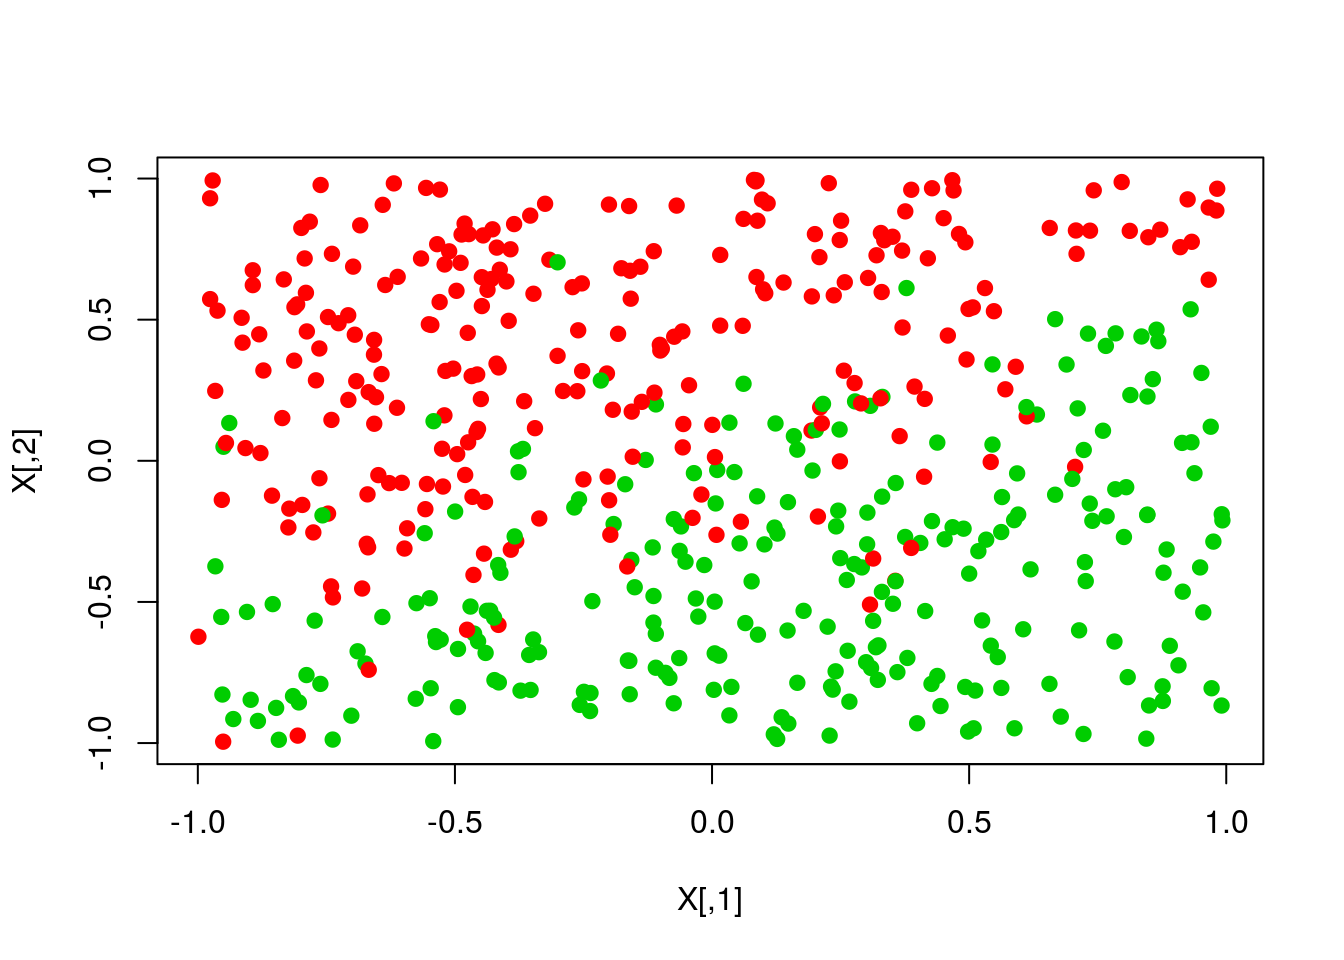
\includegraphics{04_bioconductor_files/figure-latex/unnamed-chunk-22-1.pdf}

\subsection{NCBI ESearch}\label{ncbi-esearch}

This will look very familiar to the Python tutorial from earlier, but
with more of an ``R flavor.'' Let's look for 3 cds entries.

\begin{Shaded}
\begin{Highlighting}[]
\NormalTok{ids1 <-}\StringTok{ }\KeywordTok{esearch}\NormalTok{(}\StringTok{"CFTR AND human[Organism] AND complete"}\NormalTok{,}\DataTypeTok{db=}\StringTok{'nucleotide'}\NormalTok{,}\DataTypeTok{retmax=}\DecValTok{15}\NormalTok{,}\DataTypeTok{sort=}\StringTok{'relevance'}\NormalTok{)}
\NormalTok{ids2 <-}\StringTok{ }\KeywordTok{esearch}\NormalTok{(}\StringTok{"PKD1 AND human[Organism] AND complete"}\NormalTok{,}\DataTypeTok{db=}\StringTok{'nucleotide'}\NormalTok{,}\DataTypeTok{retmax=}\DecValTok{15}\NormalTok{,}\DataTypeTok{sort=}\StringTok{'relevance'}\NormalTok{)}
\NormalTok{ids3 <-}\StringTok{ }\KeywordTok{esearch}\NormalTok{(}\StringTok{"DMPK AND human[Organism] AND complete"}\NormalTok{,}\DataTypeTok{db=}\StringTok{'nucleotide'}\NormalTok{,}\DataTypeTok{retmax=}\DecValTok{15}\NormalTok{,}\DataTypeTok{sort=}\StringTok{'relevance'}\NormalTok{)}
\end{Highlighting}
\end{Shaded}

We can parse a particular entry into a dataframe:

\begin{Shaded}
\begin{Highlighting}[]
\NormalTok{ids_df <-}\StringTok{ }\NormalTok{reutils::}\KeywordTok{content}\NormalTok{(}\KeywordTok{esummary}\NormalTok{(ids1),}\StringTok{'parsed'}\NormalTok{)}
\end{Highlighting}
\end{Shaded}

\begin{verbatim}
## Warning: HTTP error: Status 429; Too Many Requests
\end{verbatim}

\begin{verbatim}
## Warning: Errors parsing DocumentSummary
\end{verbatim}

We can also look at the text entries for each gene:

\begin{Shaded}
\begin{Highlighting}[]
\KeywordTok{efetch}\NormalTok{(ids1[}\DecValTok{1}\NormalTok{], }\DataTypeTok{rettype =} \StringTok{"fasta"}\NormalTok{, }\DataTypeTok{retmode =} \StringTok{"text"}\NormalTok{)}
\end{Highlighting}
\end{Shaded}

\begin{verbatim}
## Warning: HTTP error: Status 429; Too Many Requests
\end{verbatim}

\begin{verbatim}
## Object of class 'efetch' 
## [1] "HTTP error: Status 429; Too Many Requests"
## EFetch query using the 'nucleotide' database.
## Query url: 'https://eutils.ncbi.nlm.nih.gov/entrez/eutils/efetch.fcgi?=efe...'
## Retrieval type: 'fasta', retrieval mode: 'text'
\end{verbatim}

\begin{Shaded}
\begin{Highlighting}[]
\KeywordTok{efetch}\NormalTok{(ids2[}\DecValTok{4}\NormalTok{], }\DataTypeTok{rettype =} \StringTok{"fasta"}\NormalTok{, }\DataTypeTok{retmode =} \StringTok{"text"}\NormalTok{)}
\end{Highlighting}
\end{Shaded}

\begin{verbatim}
## Warning: HTTP error: Status 429; Too Many Requests
\end{verbatim}

\begin{verbatim}
## Object of class 'efetch' 
## [1] "HTTP error: Status 429; Too Many Requests"
## EFetch query using the 'nucleotide' database.
## Query url: 'https://eutils.ncbi.nlm.nih.gov/entrez/eutils/efetch.fcgi?=efe...'
## Retrieval type: 'fasta', retrieval mode: 'text'
\end{verbatim}

\begin{Shaded}
\begin{Highlighting}[]
\KeywordTok{efetch}\NormalTok{(ids3[}\DecValTok{5}\NormalTok{], }\DataTypeTok{rettype =} \StringTok{"fasta"}\NormalTok{, }\DataTypeTok{retmode =} \StringTok{"text"}\NormalTok{)}
\end{Highlighting}
\end{Shaded}

\begin{verbatim}
## Warning: HTTP error: Status 429; Too Many Requests
\end{verbatim}

\begin{verbatim}
## Object of class 'efetch' 
## [1] "HTTP error: Status 429; Too Many Requests"
## EFetch query using the 'nucleotide' database.
## Query url: 'https://eutils.ncbi.nlm.nih.gov/entrez/eutils/efetch.fcgi?=efe...'
## Retrieval type: 'fasta', retrieval mode: 'text'
\end{verbatim}

These look good, so let's combine the UIDs into a vector:

\begin{Shaded}
\begin{Highlighting}[]
\NormalTok{ids <-}\StringTok{ }\KeywordTok{c}\NormalTok{(ids1[}\DecValTok{1}\NormalTok{],ids2[}\DecValTok{4}\NormalTok{],ids3[}\DecValTok{5}\NormalTok{])}
\end{Highlighting}
\end{Shaded}

Now, we can extract important information, such as the sequence, by
switching to XML mode:

\begin{Shaded}
\begin{Highlighting}[]
\NormalTok{FASTA <-}\StringTok{ }\KeywordTok{efetch}\NormalTok{(ids,}\DataTypeTok{db=}\StringTok{'nucleotide'}\NormalTok{, }\DataTypeTok{rettype =} \StringTok{"fasta"}\NormalTok{, }\DataTypeTok{retmode =} \StringTok{"xml"}\NormalTok{)}
\end{Highlighting}
\end{Shaded}

\begin{verbatim}
## Warning: HTTP error: Status 429; Too Many Requests
\end{verbatim}

\begin{Shaded}
\begin{Highlighting}[]
\NormalTok{SEQS <-}\StringTok{ }\NormalTok{FASTA$}\KeywordTok{xmlValue}\NormalTok{(}\StringTok{'//TSeq_sequence'}\NormalTok{)}
\end{Highlighting}
\end{Shaded}

But there is actually a much better way, consistent with the FASTA
tutorial above:

\begin{Shaded}
\begin{Highlighting}[]
\NormalTok{tmp <-}\StringTok{ }\KeywordTok{tempfile}\NormalTok{()}
\NormalTok{FASTA <-}\StringTok{ }\KeywordTok{efetch}\NormalTok{(ids,}\DataTypeTok{db=}\StringTok{'nucleotide'}\NormalTok{, }\DataTypeTok{rettype =} \StringTok{"fasta"}\NormalTok{, }\DataTypeTok{retmode =} \StringTok{"text"}\NormalTok{, }\DataTypeTok{outfile=}\NormalTok{tmp)}
\NormalTok{FASTA <-}\StringTok{ }\KeywordTok{readDNAStringSet}\NormalTok{(tmp)}
\end{Highlighting}
\end{Shaded}

Now, let's calculate the GC content, which is easy using a bioconductor
functoin (we'll skip over our functoin from before):

\begin{Shaded}
\begin{Highlighting}[]
\KeywordTok{letterFrequency}\NormalTok{(FASTA,}\StringTok{'GC'}\NormalTok{,}\DataTypeTok{as.prob=}\OtherTok{TRUE}\NormalTok{)}
\end{Highlighting}
\end{Shaded}

\begin{verbatim}
##               G|C
## [1,] 0.3225755543
## [2,] 0.6391795013
## [3,] 0.5959700336
\end{verbatim}

If we want the GC skew, we can use our function from before. That will
give us the same GC skew result that we got from BioPython:

\begin{Shaded}
\begin{Highlighting}[]
\NormalTok{skew <-}\StringTok{ }\KeywordTok{gc_skew}\NormalTok{(FASTA[[}\DecValTok{2}\NormalTok{]],}\DecValTok{500}\NormalTok{)}
\KeywordTok{plot_skew}\NormalTok{(skew)}
\end{Highlighting}
\end{Shaded}

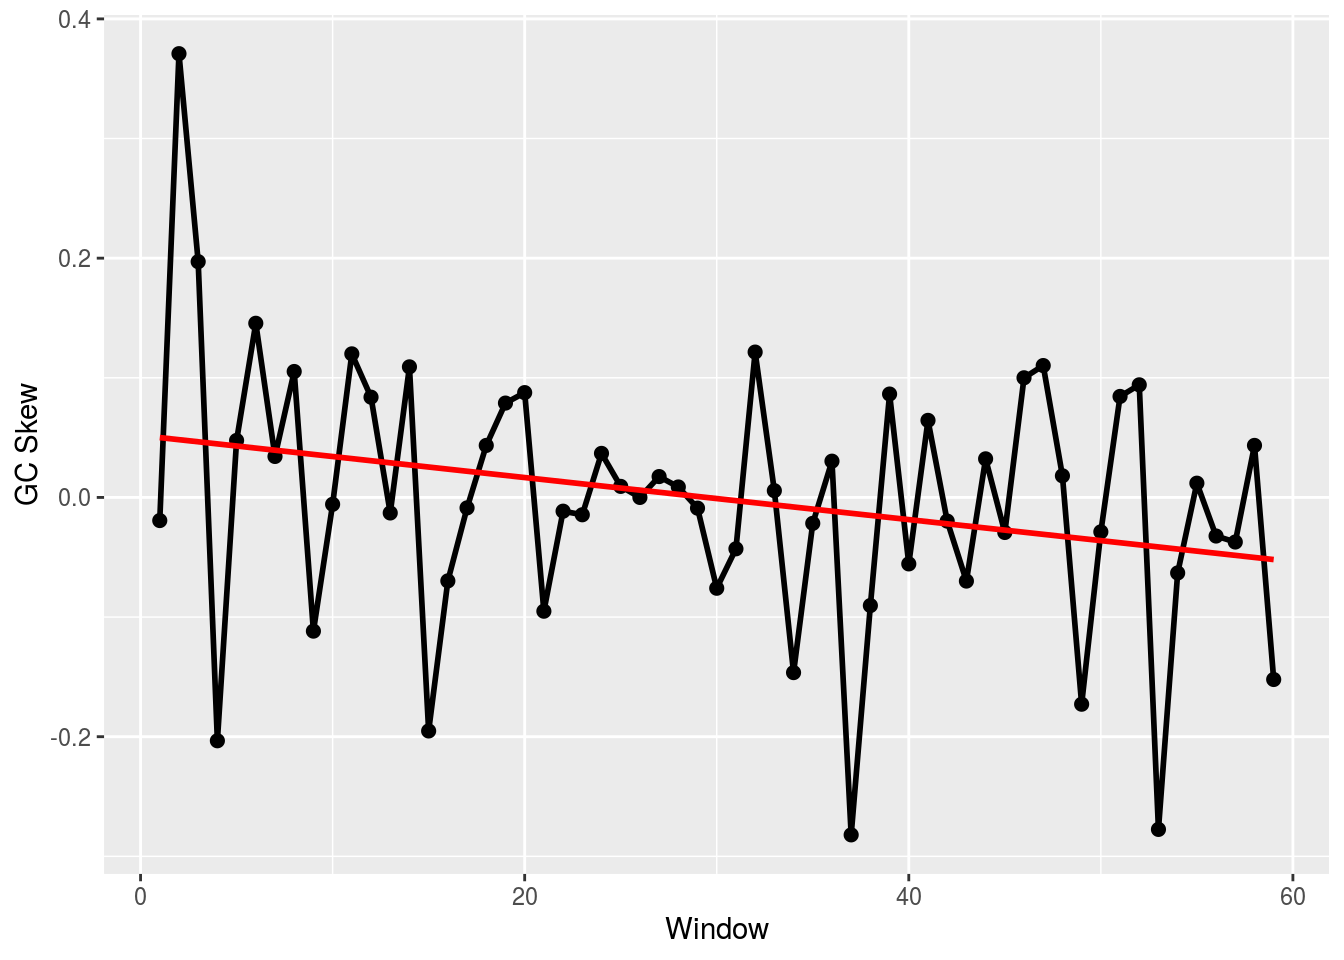
\includegraphics{04_bioconductor_files/figure-latex/unnamed-chunk-30-1.pdf}

But, we can use a function in Bioconductor. The difference betweent his
function and our implementation (and hence BioPython's) is the way the
window is defined. BioPython's were not overlapping; here they are.

\begin{Shaded}
\begin{Highlighting}[]
\NormalTok{skew <-}\StringTok{ }\KeywordTok{lapply}\NormalTok{(}\KeywordTok{seq_along}\NormalTok{(FASTA), function(i,w) \{}
  \NormalTok{numer <-}\StringTok{ }\KeywordTok{letterFrequencyInSlidingView}\NormalTok{(FASTA[[i]],}\StringTok{'G'}\NormalTok{,}\DataTypeTok{view.width=}\NormalTok{w) -}
\StringTok{    }\KeywordTok{letterFrequencyInSlidingView}\NormalTok{(FASTA[[i]],}\StringTok{'C'}\NormalTok{,}\DataTypeTok{view.width=}\NormalTok{w)}
  \NormalTok{denom <-}\StringTok{ }\KeywordTok{letterFrequencyInSlidingView}\NormalTok{(FASTA[[i]],}\StringTok{'GC'}\NormalTok{,}\DataTypeTok{view.width=}\NormalTok{w)}
  \NormalTok{numer/denom}
\NormalTok{\},}\DataTypeTok{w=}\DecValTok{500}\NormalTok{)}

\KeywordTok{plot_skew}\NormalTok{(skew[[}\DecValTok{2}\NormalTok{]])}
\end{Highlighting}
\end{Shaded}

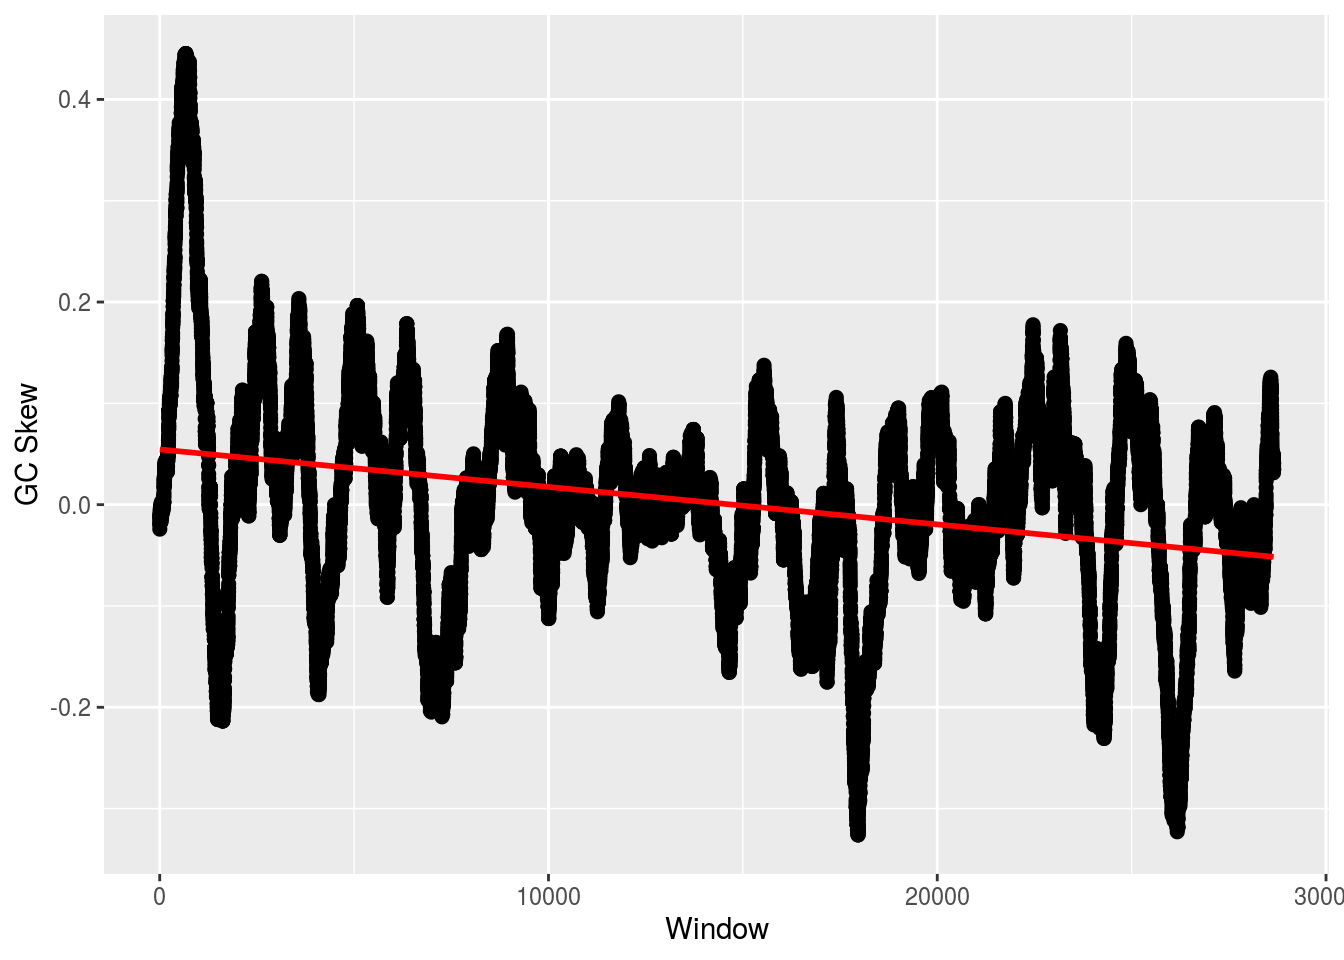
\includegraphics{04_bioconductor_files/figure-latex/unnamed-chunk-31-1.pdf}

\subsection{CDS}\label{cds}

\begin{Shaded}
\begin{Highlighting}[]
\NormalTok{ID <-}\StringTok{ }\KeywordTok{esearch}\NormalTok{(}\StringTok{"Galdieria sulphuraria[Organism] AND whole genome"}\NormalTok{,}\DataTypeTok{db=}\StringTok{'nucleotide'}\NormalTok{,}\DataTypeTok{retmax=}\DecValTok{5}\NormalTok{,}\DataTypeTok{sort=}\StringTok{'relevance'}\NormalTok{)}
\NormalTok{rec <-}\StringTok{ }\KeywordTok{efetch}\NormalTok{(ID[}\DecValTok{1}\NormalTok{],}\DataTypeTok{db=}\StringTok{'nucleotide'}\NormalTok{, }\DataTypeTok{rettype =} \StringTok{"gb"}\NormalTok{, }\DataTypeTok{retmode =} \StringTok{"xml"}\NormalTok{)}
\NormalTok{prec <-}\StringTok{ }\NormalTok{reutils::}\KeywordTok{content}\NormalTok{(rec,}\DataTypeTok{as=}\StringTok{'text'}\NormalTok{)}
\NormalTok{prec <-}\StringTok{ }\KeywordTok{xmlParse}\NormalTok{(prec)}
\NormalTok{prec <-}\StringTok{ }\KeywordTok{xmlToList}\NormalTok{(prec)}

\NormalTok{features <-}\StringTok{ }\NormalTok{prec$GBSeq$}\StringTok{`}\DataTypeTok{GBSeq_feature-table}\StringTok{`}
\NormalTok{cds_idx <-}\StringTok{ }\KeywordTok{which}\NormalTok{(}\KeywordTok{sapply}\NormalTok{(features,function(x) x[[}\DecValTok{1}\NormalTok{]]) ==}\StringTok{ 'CDS'}\NormalTok{)}
\NormalTok{features <-}\StringTok{ }\NormalTok{features[cds_idx]}

\NormalTok{features <-}\StringTok{ }\KeywordTok{lapply}\NormalTok{(features,cleanup_feat_table)}
\KeywordTok{na.omit}\NormalTok{(}\KeywordTok{sapply}\NormalTok{(features,function(x) }\KeywordTok{ifelse}\NormalTok{(}\KeywordTok{grepl}\NormalTok{(}\StringTok{'ATPase'}\NormalTok{,x[}\StringTok{'product'}\NormalTok{]),x[}\StringTok{'protein_id'}\NormalTok{],}\OtherTok{NA}\NormalTok{)))}
\end{Highlighting}
\end{Shaded}

\begin{verbatim}
## named list()
\end{verbatim}

\subsection{Whole Genomes}\label{whole-genomes}

A nice thing about Bioconductor is how easy it is to access genomic
information. Bioconductor has a pacakge called `BSgenome' that contains
complete genomes of a ton of organisms. Simply look:

\begin{Shaded}
\begin{Highlighting}[]
\KeywordTok{available.genomes}\NormalTok{() }
\end{Highlighting}
\end{Shaded}

\begin{verbatim}
##  [1] "BSgenome.Alyrata.JGI.v1"                  
##  [2] "BSgenome.Amellifera.BeeBase.assembly4"    
##  [3] "BSgenome.Amellifera.UCSC.apiMel2"         
##  [4] "BSgenome.Amellifera.UCSC.apiMel2.masked"  
##  [5] "BSgenome.Aofficinalis.NCBI.V1"            
##  [6] "BSgenome.Athaliana.TAIR.04232008"         
##  [7] "BSgenome.Athaliana.TAIR.TAIR9"            
##  [8] "BSgenome.Btaurus.UCSC.bosTau3"            
##  [9] "BSgenome.Btaurus.UCSC.bosTau3.masked"     
## [10] "BSgenome.Btaurus.UCSC.bosTau4"            
## [11] "BSgenome.Btaurus.UCSC.bosTau4.masked"     
## [12] "BSgenome.Btaurus.UCSC.bosTau6"            
## [13] "BSgenome.Btaurus.UCSC.bosTau6.masked"     
## [14] "BSgenome.Btaurus.UCSC.bosTau8"            
## [15] "BSgenome.Btaurus.UCSC.bosTau9"            
## [16] "BSgenome.Carietinum.NCBI.v1"              
## [17] "BSgenome.Celegans.UCSC.ce10"              
## [18] "BSgenome.Celegans.UCSC.ce11"              
## [19] "BSgenome.Celegans.UCSC.ce2"               
## [20] "BSgenome.Celegans.UCSC.ce6"               
## [21] "BSgenome.Cfamiliaris.UCSC.canFam2"        
## [22] "BSgenome.Cfamiliaris.UCSC.canFam2.masked" 
## [23] "BSgenome.Cfamiliaris.UCSC.canFam3"        
## [24] "BSgenome.Cfamiliaris.UCSC.canFam3.masked" 
## [25] "BSgenome.Cjacchus.UCSC.calJac3"           
## [26] "BSgenome.Dmelanogaster.UCSC.dm2"          
## [27] "BSgenome.Dmelanogaster.UCSC.dm2.masked"   
## [28] "BSgenome.Dmelanogaster.UCSC.dm3"          
## [29] "BSgenome.Dmelanogaster.UCSC.dm3.masked"   
## [30] "BSgenome.Dmelanogaster.UCSC.dm6"          
## [31] "BSgenome.Drerio.UCSC.danRer10"            
## [32] "BSgenome.Drerio.UCSC.danRer11"            
## [33] "BSgenome.Drerio.UCSC.danRer5"             
## [34] "BSgenome.Drerio.UCSC.danRer5.masked"      
## [35] "BSgenome.Drerio.UCSC.danRer6"             
## [36] "BSgenome.Drerio.UCSC.danRer6.masked"      
## [37] "BSgenome.Drerio.UCSC.danRer7"             
## [38] "BSgenome.Drerio.UCSC.danRer7.masked"      
## [39] "BSgenome.Ecoli.NCBI.20080805"             
## [40] "BSgenome.Gaculeatus.UCSC.gasAcu1"         
## [41] "BSgenome.Gaculeatus.UCSC.gasAcu1.masked"  
## [42] "BSgenome.Ggallus.UCSC.galGal3"            
## [43] "BSgenome.Ggallus.UCSC.galGal3.masked"     
## [44] "BSgenome.Ggallus.UCSC.galGal4"            
## [45] "BSgenome.Ggallus.UCSC.galGal4.masked"     
## [46] "BSgenome.Ggallus.UCSC.galGal5"            
## [47] "BSgenome.Ggallus.UCSC.galGal6"            
## [48] "BSgenome.Hsapiens.1000genomes.hs37d5"     
## [49] "BSgenome.Hsapiens.NCBI.GRCh38"            
## [50] "BSgenome.Hsapiens.UCSC.hg17"              
## [51] "BSgenome.Hsapiens.UCSC.hg17.masked"       
## [52] "BSgenome.Hsapiens.UCSC.hg18"              
## [53] "BSgenome.Hsapiens.UCSC.hg18.masked"       
## [54] "BSgenome.Hsapiens.UCSC.hg19"              
## [55] "BSgenome.Hsapiens.UCSC.hg19.masked"       
## [56] "BSgenome.Hsapiens.UCSC.hg38"              
## [57] "BSgenome.Hsapiens.UCSC.hg38.masked"       
## [58] "BSgenome.Mdomestica.UCSC.monDom5"         
## [59] "BSgenome.Mfascicularis.NCBI.5.0"          
## [60] "BSgenome.Mfuro.UCSC.musFur1"              
## [61] "BSgenome.Mmulatta.UCSC.rheMac10"          
## [62] "BSgenome.Mmulatta.UCSC.rheMac2"           
## [63] "BSgenome.Mmulatta.UCSC.rheMac2.masked"    
## [64] "BSgenome.Mmulatta.UCSC.rheMac3"           
## [65] "BSgenome.Mmulatta.UCSC.rheMac3.masked"    
## [66] "BSgenome.Mmulatta.UCSC.rheMac8"           
## [67] "BSgenome.Mmusculus.UCSC.mm10"             
## [68] "BSgenome.Mmusculus.UCSC.mm10.masked"      
## [69] "BSgenome.Mmusculus.UCSC.mm8"              
## [70] "BSgenome.Mmusculus.UCSC.mm8.masked"       
## [71] "BSgenome.Mmusculus.UCSC.mm9"              
## [72] "BSgenome.Mmusculus.UCSC.mm9.masked"       
## [73] "BSgenome.Osativa.MSU.MSU7"                
## [74] "BSgenome.Ptroglodytes.UCSC.panTro2"       
## [75] "BSgenome.Ptroglodytes.UCSC.panTro2.masked"
## [76] "BSgenome.Ptroglodytes.UCSC.panTro3"       
## [77] "BSgenome.Ptroglodytes.UCSC.panTro3.masked"
## [78] "BSgenome.Ptroglodytes.UCSC.panTro5"       
## [79] "BSgenome.Ptroglodytes.UCSC.panTro6"       
## [80] "BSgenome.Rnorvegicus.UCSC.rn4"            
## [81] "BSgenome.Rnorvegicus.UCSC.rn4.masked"     
## [82] "BSgenome.Rnorvegicus.UCSC.rn5"            
## [83] "BSgenome.Rnorvegicus.UCSC.rn5.masked"     
## [84] "BSgenome.Rnorvegicus.UCSC.rn6"            
## [85] "BSgenome.Scerevisiae.UCSC.sacCer1"        
## [86] "BSgenome.Scerevisiae.UCSC.sacCer2"        
## [87] "BSgenome.Scerevisiae.UCSC.sacCer3"        
## [88] "BSgenome.Sscrofa.UCSC.susScr11"           
## [89] "BSgenome.Sscrofa.UCSC.susScr3"            
## [90] "BSgenome.Sscrofa.UCSC.susScr3.masked"     
## [91] "BSgenome.Tgondii.ToxoDB.7.0"              
## [92] "BSgenome.Tguttata.UCSC.taeGut1"           
## [93] "BSgenome.Tguttata.UCSC.taeGut1.masked"    
## [94] "BSgenome.Tguttata.UCSC.taeGut2"           
## [95] "BSgenome.Vvinifera.URGI.IGGP12Xv0"        
## [96] "BSgenome.Vvinifera.URGI.IGGP12Xv2"        
## [97] "BSgenome.Vvinifera.URGI.IGGP8X"
\end{verbatim}

We can install a specific genomes and parse them quite easily:

\begin{Shaded}
\begin{Highlighting}[]
\KeywordTok{load_library}\NormalTok{(BSgenome.Athaliana.TAIR}\FloatTok{.04232008}\NormalTok{)}
\end{Highlighting}
\end{Shaded}

For example, to calculate the GC content of each chromosome in either
genome, we can do the following:

\begin{Shaded}
\begin{Highlighting}[]
\NormalTok{params <-}\StringTok{ }\KeywordTok{new}\NormalTok{(}\StringTok{'BSParams'}\NormalTok{,}
              \DataTypeTok{X=}\NormalTok{Athaliana,}
              \DataTypeTok{FUN =} \NormalTok{function(x) }\KeywordTok{letterFrequency}\NormalTok{(x,}\StringTok{'GC'}\NormalTok{,}\DataTypeTok{as.prob=}\OtherTok{TRUE}\NormalTok{),}
              \DataTypeTok{exclude=}\KeywordTok{c}\NormalTok{(}\StringTok{'M'}\NormalTok{,}\StringTok{'C'}\NormalTok{))}
\KeywordTok{unlist}\NormalTok{(}\KeywordTok{bsapply}\NormalTok{(params))}
\end{Highlighting}
\end{Shaded}

\begin{verbatim}
##     chr1.G|C     chr2.G|C     chr3.G|C     chr4.G|C     chr5.G|C 
## 0.3567394241 0.3584669531 0.3630477097 0.3619816947 0.3590229191
\end{verbatim}

\section{Retrieving Projects}\label{sra}

Many of your projects will involve working with publically available
data from published research. The data itself is typicaly uploaded to a
data repository like NCBI or EMBL/EBI. The files are deposited as
Sequence Read Archive (SRA) files and are often searchable as
bioprojects. Accessing these files can be accomplished using
Bioconductor in R.

\begin{Shaded}
\begin{Highlighting}[]
\KeywordTok{library}\NormalTok{(stringr)}
\KeywordTok{library}\NormalTok{(SRAdb)}
\KeywordTok{library}\NormalTok{(Biostrings)}
\end{Highlighting}
\end{Shaded}

First, download the database file to your working director via

\begin{Shaded}
\begin{Highlighting}[]
\KeywordTok{getSRAdbFile}\NormalTok{(}\DataTypeTok{destdir=}\KeywordTok{getwd}\NormalTok{(),}\DataTypeTok{destfile=}\StringTok{'SRAmetadb.sqlite.gz'}\NormalTok{,method)}
\end{Highlighting}
\end{Shaded}

Then, we'll make a connection with the database:

\begin{Shaded}
\begin{Highlighting}[]
\NormalTok{sqlfile <-}\StringTok{ '~/SRAmetadb.sqlite'}
\NormalTok{sra_con <-}\StringTok{ }\KeywordTok{dbConnect}\NormalTok{(}\KeywordTok{SQLite}\NormalTok{(),sqlfile)}
\end{Highlighting}
\end{Shaded}

Let's assume we want to download the data from the Gevers IBD study that
was deposited with the following accession: PRJNA237362. We can see this
project on NCBI here:
\url{https://www.ncbi.nlm.nih.gov/bioproject/PRJNA237362} . If we click
the link next to `SRA Experiments' and then click one of the sample
links on the subsequent page, we'll end up on a page that looks like
this: \url{https://www.ncbi.nlm.nih.gov/sra/SRX1418176\%5Baccn\%5D} .
Here' we can access the SRA project code: SRP040765. This is what we
need.

Before we continue, let me go over the SRA file types:

\begin{itemize}
\tightlist
\item
  SRA - Accession information that contains the 5 files below
\item
  SRP - Project information and metadata
\item
  SRS - Sample metadata
\item
  SRX - Experiment metadata including library, platform selection, and
  processing parametes involved in a particular sequencing experiment
\item
  SRR - Sequencing run information
\item
  SRX - Sequence analysis BAM file information
\end{itemize}

Now that we have the SRP, let's acquire the files we need, specifically
the SRA files:

\begin{Shaded}
\begin{Highlighting}[]
\NormalTok{rs <-}\StringTok{ }\KeywordTok{listSRAfile}\NormalTok{(}\KeywordTok{c}\NormalTok{(}\StringTok{'SRP040765'}\NormalTok{), sra_con, }\DataTypeTok{fileType =} \StringTok{'sra'}\NormalTok{)}
\KeywordTok{str}\NormalTok{(rs)}
\end{Highlighting}
\end{Shaded}

\begin{verbatim}
## 'data.frame':    3408 obs. of  5 variables:
##  $ study     : chr  "SRP040765" "SRP040765" "SRP040765" "SRP040765" ...
##  $ sample    : chr  "SRS587325" "SRS587957" "SRS587956" "SRS695027" ...
##  $ experiment: chr  "SRX691644" "SRX692390" "SRX509287" "SRX693364" ...
##  $ run       : chr  "SRR1564534" "SRR1565230" "SRR1215330" "SRR1566410" ...
##  $ ftp       : chr  "ftp://ftp-trace.ncbi.nlm.nih.gov/sra/sra-instant/reads/ByRun/sra/SRR/SRR156/SRR1564534/SRR1564534.sra" "ftp://ftp-trace.ncbi.nlm.nih.gov/sra/sra-instant/reads/ByRun/sra/SRR/SRR156/SRR1565230/SRR1565230.sra" "ftp://ftp-trace.ncbi.nlm.nih.gov/sra/sra-instant/reads/ByRun/sra/SRR/SRR121/SRR1215330/SRR1215330.sra" "ftp://ftp-trace.ncbi.nlm.nih.gov/sra/sra-instant/reads/ByRun/sra/SRR/SRR156/SRR1566410/SRR1566410.sra" ...
\end{verbatim}

\textbf{rs} is a dataframe containing the SRP, SRS, SRX, and SRR IDs for
a given sequencing run, as well as the ftp link to the actual .sra file
containing the sequencing information. These are the links we can use to
download the entire set of data we need to perform some analysis.

Now, we could export these links and then just iterate through, maybe
using bash with wget, to download all of these files. Alternatively, we
can do the following:

We'll get a run ID for a run we'ld like to download:

\begin{Shaded}
\begin{Highlighting}[]
\NormalTok{run <-}\StringTok{ }\NormalTok{rs$run[}\DecValTok{1}\NormalTok{]}
\NormalTok{run}
\end{Highlighting}
\end{Shaded}

\begin{verbatim}
## [1] "SRR1564534"
\end{verbatim}

If we want the specific SRR (run) information, we do:

\begin{Shaded}
\begin{Highlighting}[]
\NormalTok{run_info <-}\StringTok{ }\KeywordTok{getSRA}\NormalTok{(}\DataTypeTok{search_terms=}\StringTok{'SRP040765'}\NormalTok{, }\DataTypeTok{out_types=}\KeywordTok{c}\NormalTok{(}\StringTok{'run'}\NormalTok{),sra_con)}
\KeywordTok{str}\NormalTok{(run_info)}
\end{Highlighting}
\end{Shaded}

\begin{verbatim}
## 'data.frame':    3408 obs. of  11 variables:
##  $ run_alias      : chr  "A21YN121012.1.Illumina_P7-Fexexoja.screened.bam" "A21YN121012.1.Illumina_P7-Wodejora.screened.bam" "A2WP7130403.1.Illumina_P7-Xakokoxe.screened.bam" "A1UEN121219.1.Illumina_P7-Birarane.screened.bam" ...
##  $ run            : chr  "SRR1564534" "SRR1565230" "SRR1215330" "SRR1566410" ...
##  $ run_date       : chr  "2012-10-12" "2012-10-12" "2013-04-03" "2012-12-19" ...
##  $ updated_date   : chr  "2014-09-04" "2014-09-05" "2019-12-11" "2014-09-06" ...
##  $ spots          : num  120 449 2102 9532 676152 ...
##  $ bases          : num  4.20e+04 1.57e+05 7.36e+05 3.34e+06 1.37e+08 ...
##  $ run_center     : chr  "BI" "BI" "BI" "BI" ...
##  $ experiment_name: logi  NA NA NA NA NA NA ...
##  $ run_url_link   : logi  NA NA NA NA NA NA ...
##  $ run_entrez_link: logi  NA NA NA NA NA NA ...
##  $ run_attribute  : chr  "analysis_type: AssemblyWithoutReference || flowcell_barcode: A21YN || gssr_id: 247611.0 || instrument_name: SL-"| __truncated__ "analysis_type: AssemblyWithoutReference || flowcell_barcode: A21YN || gssr_id: 247629.0 || instrument_name: SL-"| __truncated__ "analysis_type: AssemblyWithoutReference || flowcell_barcode: A2WP7 || gssr_id: 247671.0 || instrument_name: SL-"| __truncated__ "analysis_type: AssemblyWithoutReference || data_type: 16S || flowcell_barcode: A1UEN || gssr_id: 276389.0 || in"| __truncated__ ...
\end{verbatim}

and for the SRS (sample) information:

\begin{Shaded}
\begin{Highlighting}[]
\NormalTok{sample_info <-}\StringTok{ }\KeywordTok{getSRA}\NormalTok{(}\DataTypeTok{search_terms=}\StringTok{'SRP040765'}\NormalTok{, }\DataTypeTok{out_types=}\KeywordTok{c}\NormalTok{(}\StringTok{'sample'}\NormalTok{),sra_con)}
\KeywordTok{str}\NormalTok{(sample_info)}
\end{Highlighting}
\end{Shaded}

\begin{verbatim}
## 'data.frame':    1572 obs. of  10 variables:
##  $ sample_alias      : chr  "SKBTI-0107" "SKBTI-0128" "SKBTI-0172" "SKBTI-0594" ...
##  $ sample            : chr  "SRS587325" "SRS587957" "SRS587956" "SRS695027" ...
##  $ taxon_id          : int  408170 408170 408170 408170 408170 408170 408170 408170 408170 408170 ...
##  $ common_name       : chr  NA NA NA NA ...
##  $ anonymized_name   : chr  NA NA NA NA ...
##  $ individual_name   : chr  NA NA NA NA ...
##  $ description       : logi  NA NA NA NA NA NA ...
##  $ sample_url_link   : logi  NA NA NA NA NA NA ...
##  $ sample_entrez_link: logi  NA NA NA NA NA NA ...
##  $ sample_attribute  : chr  "strain: SKBTI-0107 || collection date: missing || geographic location (country and/or sea, region): USA || spec"| __truncated__ "strain: SKBTI-0128 || collection date: missing || geographic location (country and/or sea, region): USA || spec"| __truncated__ "strain: SKBTI-0172 || collection date: missing || geographic location (country and/or sea, region): USA || spec"| __truncated__ "strain: SKBTI-0594 || collection date: missing || geographic location (country and/or sea, region): USA || spec"| __truncated__ ...
\end{verbatim}

and SRX (experiment) information:

\begin{Shaded}
\begin{Highlighting}[]
\NormalTok{experiment_info <-}\StringTok{ }\KeywordTok{getSRA}\NormalTok{(}\DataTypeTok{search_terms=}\StringTok{'SRP040765'}\NormalTok{, }\DataTypeTok{out_types=}\KeywordTok{c}\NormalTok{(}\StringTok{'experiment'}\NormalTok{),sra_con)}
\KeywordTok{str}\NormalTok{(experiment_info)}
\end{Highlighting}
\end{Shaded}

\begin{verbatim}
## 'data.frame':    2708 obs. of  27 variables:
##  $ experiment_alias             : chr  "2949006.WR32770.Solexa-122962.A21YN121012.P" "2949006.WR32770.Solexa-122980.A21YN121012.P" "2949006.WR32770.Solexa-123022.A2WP7130403.P" "2949006.WR33991.Solexa-133729.A1UEN121219.P" ...
##  $ experiment                   : chr  "SRX691644" "SRX692390" "SRX509287" "SRX693364" ...
##  $ experiment_title             : chr  "Illumina amplicon sequencing of metagenomic paired-end library 'Solexa-122962' containing sample 'SKBTI-0107'" "Illumina amplicon sequencing of metagenomic paired-end library 'Solexa-122980' containing sample 'SKBTI-0128'" "Illumina amplicon sequencing of metagenomic paired-end library 'Solexa-123022' containing sample 'SKBTI-0172'" "Illumina amplicon sequencing of metagenomic paired-end library 'Solexa-133729' containing sample 'SKBTI-0594'" ...
##  $ study_name                   : logi  NA NA NA NA NA NA ...
##  $ sample_name                  : logi  NA NA NA NA NA NA ...
##  $ design_description           : chr  "Illumina sequencing of human gut metagenome via polymerase chain reaction" "Illumina sequencing of human gut metagenome via polymerase chain reaction" "Illumina sequencing of human gut metagenome via polymerase chain reaction" "Illumina sequencing of human gut metagenome via polymerase chain reaction" ...
##  $ library_name                 : chr  "Solexa-122962" "Solexa-122980" "Solexa-123022" "Solexa-133729" ...
##  $ library_strategy             : chr  "AMPLICON" "AMPLICON" "AMPLICON" "AMPLICON" ...
##  $ library_source               : chr  "METAGENOMIC" "METAGENOMIC" "METAGENOMIC" "METAGENOMIC" ...
##  $ library_selection            : chr  "PCR" "PCR" "PCR" "PCR" ...
##  $ library_layout               : chr  "PAIRED - NOMINAL_SDEV: 0.0E0; NOMINAL_LENGTH: 390; " "PAIRED - NOMINAL_SDEV: 0.0E0; NOMINAL_LENGTH: 390; " "PAIRED - NOMINAL_SDEV: 0.0E0; NOMINAL_LENGTH: 393; " "PAIRED - NOMINAL_SDEV: 0.0E0; NOMINAL_LENGTH: 382; " ...
##  $ library_construction_protocol: logi  NA NA NA NA NA NA ...
##  $ adapter_spec                 : logi  NA NA NA NA NA NA ...
##  $ read_spec                    : chr  "READ_INDEX: 0; READ_LABEL: forward; READ_CLASS: Application Read; READ_TYPE: Forward; BASE_COORD: 1 || READ_IND"| __truncated__ "READ_INDEX: 0; READ_LABEL: forward; READ_CLASS: Application Read; READ_TYPE: Forward; BASE_COORD: 1 || READ_IND"| __truncated__ "READ_INDEX: 0; READ_LABEL: forward; READ_CLASS: Application Read; READ_TYPE: Forward; BASE_COORD: 1 || READ_IND"| __truncated__ "READ_INDEX: 0; READ_LABEL: forward; READ_CLASS: Application Read; READ_TYPE: Forward; BASE_COORD: 1 || READ_IND"| __truncated__ ...
##  $ platform                     : chr  "ILLUMINA" "ILLUMINA" "ILLUMINA" "ILLUMINA" ...
##  $ instrument_model             : chr  "Illumina MiSeq" "Illumina MiSeq" "Illumina MiSeq" "Illumina MiSeq" ...
##  $ instrument_name              : logi  NA NA NA NA NA NA ...
##  $ platform_parameters          : chr  "INSTRUMENT_MODEL: Illumina MiSeq" "INSTRUMENT_MODEL: Illumina MiSeq" "INSTRUMENT_MODEL: Illumina MiSeq" "INSTRUMENT_MODEL: Illumina MiSeq" ...
##  $ sequence_space               : logi  NA NA NA NA NA NA ...
##  $ base_caller                  : logi  NA NA NA NA NA NA ...
##  $ quality_scorer               : logi  NA NA NA NA NA NA ...
##  $ number_of_levels             : logi  NA NA NA NA NA NA ...
##  $ multiplier                   : logi  NA NA NA NA NA NA ...
##  $ qtype                        : logi  NA NA NA NA NA NA ...
##  $ experiment_url_link          : logi  NA NA NA NA NA NA ...
##  $ experiment_entrez_link       : logi  NA NA NA NA NA NA ...
##  $ experiment_attribute         : chr  "analysis_type: AssemblyWithoutReference || gssr_id: 247611.0 || library_type: 16S || lsid: broadinstitute.org:b"| __truncated__ "analysis_type: AssemblyWithoutReference || gssr_id: 247629.0 || library_type: 16S || lsid: broadinstitute.org:b"| __truncated__ "analysis_type: AssemblyWithoutReference || gssr_id: 247671.0 || library_type: 16S || lsid: broadinstitute.org:b"| __truncated__ "analysis_type: AssemblyWithoutReference || data_type: 16S || gssr_id: 276389.0 || library_type: 16S || lsid: br"| __truncated__ ...
\end{verbatim}

Using these commands, you should be able to download the .sra files you
need along with all corresponding metadata to do analysis. Still, you
might be wondering how you get the .fasta files from the .sra file.
Well, the easiest way is to use something called the sra toolkit, which
can be found here: \url{https://www.ncbi.nlm.nih.gov/books/NBK158900/} .

So let's say we aimed to extract the sequences from the following sra
files: SRR1635768 and SRR1566401. First, we'd download the files:

\begin{Shaded}
\begin{Highlighting}[]
\NormalTok{sra_dir <-}\StringTok{ }\KeywordTok{tempdir}\NormalTok{()}

\NormalTok{sra_fns <-}\StringTok{ }\KeywordTok{c}\NormalTok{(}\StringTok{"SRR1634425"}\NormalTok{,}\StringTok{"SRR1634428"}\NormalTok{)}
\NormalTok{for (sra in sra_fns) }\KeywordTok{getSRAfile}\NormalTok{(sra, sra_con, }\DataTypeTok{fileType =} \StringTok{'sra'}\NormalTok{,}\DataTypeTok{destDir=}\NormalTok{sra_dir)}
\end{Highlighting}
\end{Shaded}

\begin{verbatim}
## Files are saved to: 
## '/tmp/Rtmp3MctDm'
## 
## Files are saved to: 
## '/tmp/Rtmp3MctDm'
\end{verbatim}

Then, we'd use the sra toolkit to extract the sequences. Assuming you
have downloaded and installed it, we can do the following

\begin{Shaded}
\begin{Highlighting}[]
\NormalTok{sra_output <-}\StringTok{ }\KeywordTok{tempdir}\NormalTok{()}

\NormalTok{sra_files <-}\StringTok{ }\KeywordTok{list.files}\NormalTok{(sra_dir,}\DataTypeTok{full.names=}\OtherTok{TRUE}\NormalTok{,}\DataTypeTok{pattern=}\StringTok{'}\CharTok{\textbackslash{}\textbackslash{}}\StringTok{.sra$'}\NormalTok{)}

\NormalTok{for (i in }\KeywordTok{seq_along}\NormalTok{(sra_files)) }\KeywordTok{system2}\NormalTok{(}\StringTok{'fastq-dump'}\NormalTok{,}\DataTypeTok{args=}\KeywordTok{c}\NormalTok{(sra_files[i],}
                                                              \StringTok{'-O'}\NormalTok{, sra_output,}
                                                              \StringTok{'--gzip'}\NormalTok{,}
                                                              \StringTok{'--clip'}\NormalTok{,}
                                                              \StringTok{'--skip-technical'}\NormalTok{,}
                                                              \StringTok{'--dumpbase'}\NormalTok{))}
\end{Highlighting}
\end{Shaded}

And now we can check:

\begin{Shaded}
\begin{Highlighting}[]
\NormalTok{fqs <-}\StringTok{ }\KeywordTok{list.files}\NormalTok{(sra_output,}\DataTypeTok{full.names=}\OtherTok{TRUE}\NormalTok{)}

\NormalTok{FASTQ <-}\StringTok{ }\KeywordTok{readDNAStringSet}\NormalTok{(fqs,}\DataTypeTok{format=}\StringTok{'fastq'}\NormalTok{)}
\NormalTok{FASTQ}
\end{Highlighting}
\end{Shaded}

Note the header names; they're simply the SRR ids. You'd have to the sra
metadata (see above) to match these to specific samples. For example,

\begin{Shaded}
\begin{Highlighting}[]
\NormalTok{sample_info <-}\StringTok{ }\KeywordTok{getSRA}\NormalTok{(}\DataTypeTok{search_terms=}\StringTok{'SRR1635768'}\NormalTok{, }\DataTypeTok{out_types=}\KeywordTok{c}\NormalTok{(}\StringTok{'sample'}\NormalTok{),sra_con)}
\KeywordTok{str}\NormalTok{(sample_info)}
\end{Highlighting}
\end{Shaded}

\begin{verbatim}
## 'data.frame':    1 obs. of  10 variables:
##  $ sample_alias      : chr "SKBTI-0325"
##  $ sample            : chr "SRS734393"
##  $ taxon_id          : int 408170
##  $ common_name       : logi NA
##  $ anonymized_name   : logi NA
##  $ individual_name   : logi NA
##  $ description       : logi NA
##  $ sample_url_link   : logi NA
##  $ sample_entrez_link: logi NA
##  $ sample_attribute  : chr "strain: SKBTI-0325 || collection date: missing || geographic location (country and/or sea, region): USA || spec"| __truncated__
\end{verbatim}

\subsubsection{Fastq Dump for Paired End
Reads}\label{fastq-dump-for-paired-end-reads}

It should be noted that simply using the fastq-dump command as above
works only if your data \emph{does not consist of paired end reads}. If
you happen to have paired end reads, then the following arguments must
be added to the fastq-dump call:

\begin{Shaded}
\begin{Highlighting}[]
\NormalTok{for (i in }\KeywordTok{seq_along}\NormalTok{(sra_files)) }\KeywordTok{system2}\NormalTok{(}\StringTok{'fastq-dump'}\NormalTok{,}\DataTypeTok{args=}\KeywordTok{c}\NormalTok{(sra_files[i],}
                                                              \StringTok{'-O'}\NormalTok{, sra_output,}
                                                              \StringTok{'--gzip'}\NormalTok{,}
                                                              \StringTok{'--clip'}\NormalTok{,}
                                                              \StringTok{'--skip-technical'}\NormalTok{,}
                                                              \StringTok{'--dumpbase'}\NormalTok{,}
                                                              \StringTok{'--split-files'}\NormalTok{,}
                                                              \StringTok{'--readids'}\NormalTok{))}
\end{Highlighting}
\end{Shaded}

For more information, see
\url{https://edwards.sdsu.edu/research/fastq-dump/}

\section{Phyloseq}\label{phyloseq}

For downstream metagenomic analysis, you cannot go wrong with Phyloseq.
It's an excellent tool for importing and analyzing metagenomic data, and
acts as a wrapper for a considerable number of well known tools and
packages ranging from vegan to DESeq2. Moreover, it's well equipt for
importing data you'd generate by using, say, QIIME, and works with its
own set of structures, which really comes helps prevent potential
indexing issues and the like.

\begin{Shaded}
\begin{Highlighting}[]
\KeywordTok{library}\NormalTok{(phyloseq)}
\KeywordTok{library}\NormalTok{(tidyverse)}
\KeywordTok{library}\NormalTok{(ape)}
\KeywordTok{library}\NormalTok{(DESeq2)}
\end{Highlighting}
\end{Shaded}

Let's begin by loading four pieces of data, an OTU table of taxonomic
abundances (counts), taxonomy information with the taxa that a given OTU
likely belongs to, sample metadata, and a phylogenetic tree.

\begin{Shaded}
\begin{Highlighting}[]
\NormalTok{OTU <-}\StringTok{ }\KeywordTok{read.csv}\NormalTok{(}\StringTok{'https://gist.githubusercontent.com/sw1/8870a124624f31585d5c15be72fcfc21/raw/1b05f24f189f14ea9902ac3867aca40c80ac6db3/otu_table.csv'}\NormalTok{)}
\NormalTok{TAX <-}\StringTok{ }\KeywordTok{read.csv}\NormalTok{(}\StringTok{'https://gist.githubusercontent.com/sw1/8870a124624f31585d5c15be72fcfc21/raw/1b05f24f189f14ea9902ac3867aca40c80ac6db3/tax_table.csv'}\NormalTok{)}
\NormalTok{SAMP <-}\StringTok{ }\KeywordTok{read.csv}\NormalTok{(}\StringTok{'https://gist.githubusercontent.com/sw1/8870a124624f31585d5c15be72fcfc21/raw/052dfdc3df97589f6405d79889c9b3b651eb1967/sample_metadata.csv'}\NormalTok{)}
\NormalTok{TREE <-}\StringTok{ }\KeywordTok{read.tree}\NormalTok{(}\StringTok{'https://gist.githubusercontent.com/sw1/8870a124624f31585d5c15be72fcfc21/raw/052dfdc3df97589f6405d79889c9b3b651eb1967/tree.tree'}\NormalTok{)}
\end{Highlighting}
\end{Shaded}

In most circumstances, we'd work on this as is, but the nice thing about
phyloseq is that we can place these into a phyloseq container, allowing
us to manipulate the four objects simultaneously. Imagine if we decided
to filter some OTUs based on the leaves of our tree. We'd then may want
to then remove these OTUs from our taxonomy. Also, removing a subset of
OTUs may result in some samples with 0 total OTU counts, which justifies
removing them as well. This can lead to indexing issues where we
accidentally shuffle our tables. Using phyloseq, all of this is done in
tandem, preventing said issues.

Let's create that container. We need to coerse each objects into
phyloseq-friendly objects, so note the functions wrapping each object.
Also note that our row and column names \emph{must} be consistent
throughout (i.e., named the same and in the same order). And lastly, the
taxonomy table has to be a matrix.

\begin{Shaded}
\begin{Highlighting}[]
\KeywordTok{all}\NormalTok{(}\KeywordTok{colnames}\NormalTok{(OTU) ==}\StringTok{ }\NormalTok{SAMP$Sample_ID)}
\end{Highlighting}
\end{Shaded}

\begin{verbatim}
## [1] TRUE
\end{verbatim}

\begin{Shaded}
\begin{Highlighting}[]
\KeywordTok{rownames}\NormalTok{(SAMP) <-}\StringTok{ }\NormalTok{SAMP$Sample_ID}

\NormalTok{TAX <-}\StringTok{ }\KeywordTok{as.matrix}\NormalTok{(TAX)}
\KeywordTok{rownames}\NormalTok{(TAX) <-}\StringTok{ }\KeywordTok{paste0}\NormalTok{(}\StringTok{'otu'}\NormalTok{,}\DecValTok{1}\NormalTok{:}\KeywordTok{nrow}\NormalTok{(TAX))}
\KeywordTok{rownames}\NormalTok{(OTU) <-}\StringTok{ }\KeywordTok{rownames}\NormalTok{(TAX)}

\KeywordTok{taxa_names}\NormalTok{(TREE) <-}\StringTok{ }\KeywordTok{rownames}\NormalTok{(TAX)}
\end{Highlighting}
\end{Shaded}

And now, create the phyloseq container:

\begin{Shaded}
\begin{Highlighting}[]
\NormalTok{PS <-}\StringTok{ }\KeywordTok{phyloseq}\NormalTok{(}\KeywordTok{otu_table}\NormalTok{(OTU,}\DataTypeTok{taxa_are_rows=}\OtherTok{TRUE}\NormalTok{),}\KeywordTok{tax_table}\NormalTok{(TAX),}\KeywordTok{sample_data}\NormalTok{(SAMP),}\KeywordTok{phy_tree}\NormalTok{(TREE))}
\end{Highlighting}
\end{Shaded}

First, we'll filter any samples without enterotype information and then
conver enterotype to a factor:

\begin{Shaded}
\begin{Highlighting}[]
\NormalTok{PS1 <-}\StringTok{ }\KeywordTok{prune_samples}\NormalTok{(!}\KeywordTok{is.na}\NormalTok{(}\KeywordTok{sample_data}\NormalTok{(PS)$Enterotype),PS)}
\KeywordTok{sample_data}\NormalTok{(PS1)$ENTEROTYPE <-}\StringTok{ }\KeywordTok{as.factor}\NormalTok{(}\KeywordTok{sample_data}\NormalTok{(PS1)$Enterotype)}
\end{Highlighting}
\end{Shaded}

Now, we'll remove any OTUs with 0 counts across samples:

\begin{Shaded}
\begin{Highlighting}[]
\NormalTok{PS1 <-}\StringTok{ }\KeywordTok{filter_taxa}\NormalTok{(PS1,function(x) }\KeywordTok{sum}\NormalTok{(x) >}\StringTok{ }\DecValTok{0}\NormalTok{,}\DataTypeTok{prune =} \OtherTok{TRUE}\NormalTok{)}
\end{Highlighting}
\end{Shaded}

This leaves us with the following objects:

\begin{Shaded}
\begin{Highlighting}[]
\NormalTok{PS1}
\end{Highlighting}
\end{Shaded}

\begin{verbatim}
## phyloseq-class experiment-level object
## otu_table()   OTU Table:         [ 342 taxa and 271 samples ]
## sample_data() Sample Data:       [ 271 samples by 10 sample variables ]
## tax_table()   Taxonomy Table:    [ 342 taxa by 2 taxonomic ranks ]
## phy_tree()    Phylogenetic Tree: [ 342 tips and 341 internal nodes ]
\end{verbatim}

From here, we can do quite a bit, so I'm not going to go through
absolutely everything. But, we can start with some figures. We can plot
some metagenomic summary statistics:

\begin{Shaded}
\begin{Highlighting}[]
\KeywordTok{plot_richness}\NormalTok{(PS1,}\DataTypeTok{x=}\StringTok{'ENTEROTYPE'}\NormalTok{,}\DataTypeTok{color=}\StringTok{'ENTEROTYPE'}\NormalTok{)}
\end{Highlighting}
\end{Shaded}

\begin{verbatim}
## Warning: Removed 1359 rows containing missing values (geom_errorbar).
\end{verbatim}

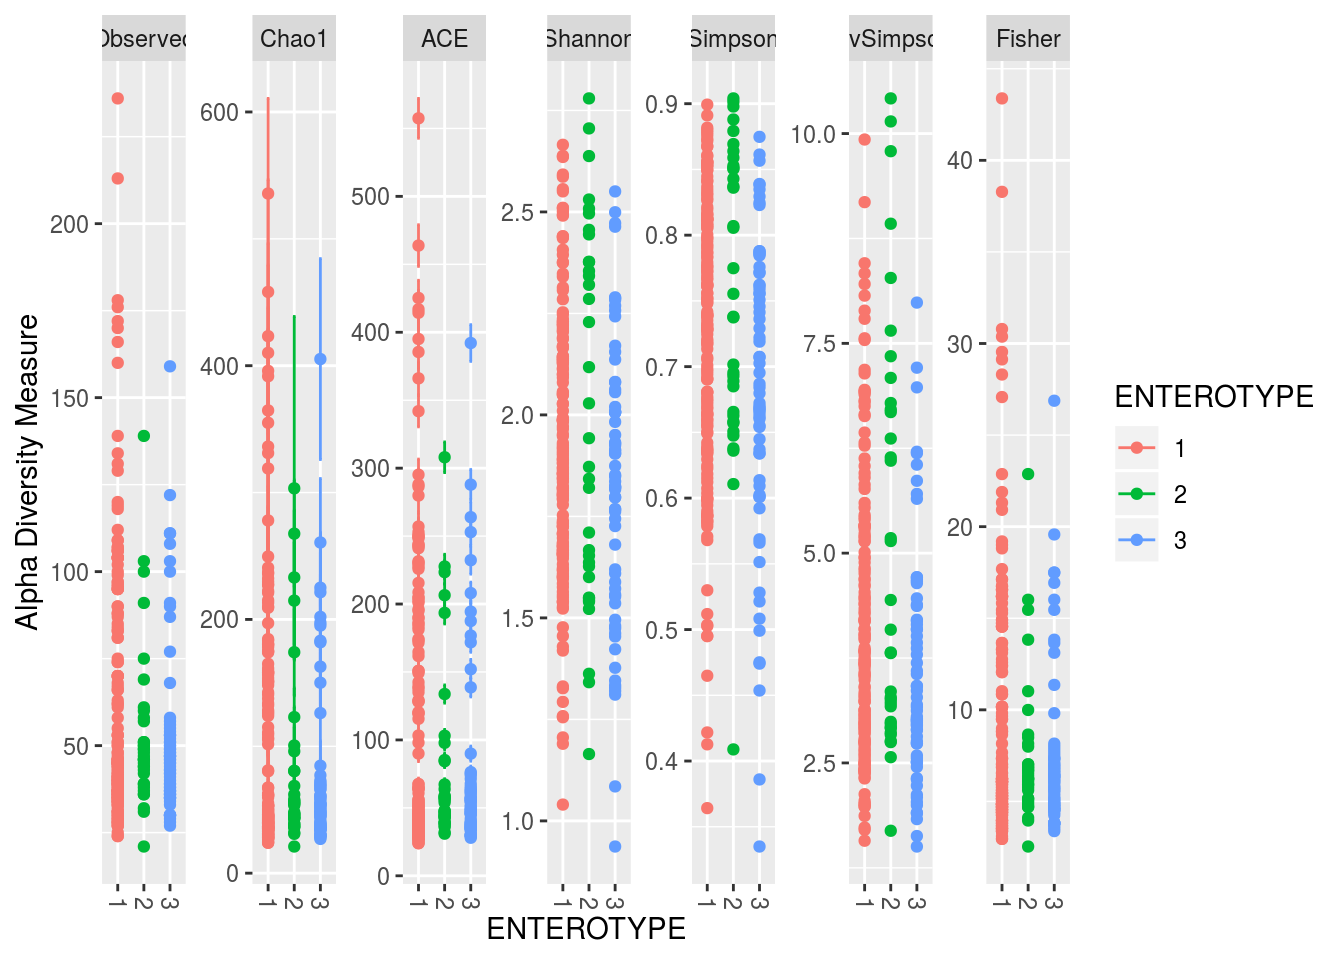
\includegraphics{06_phyloseq_files/figure-latex/unnamed-chunk-9-1.pdf}

And then some figures to show abundance in different ways:

\begin{Shaded}
\begin{Highlighting}[]
\KeywordTok{plot_tree}\NormalTok{(PS1,}\DataTypeTok{color=}\StringTok{'ENTEROTYPE'}\NormalTok{)}
\end{Highlighting}
\end{Shaded}

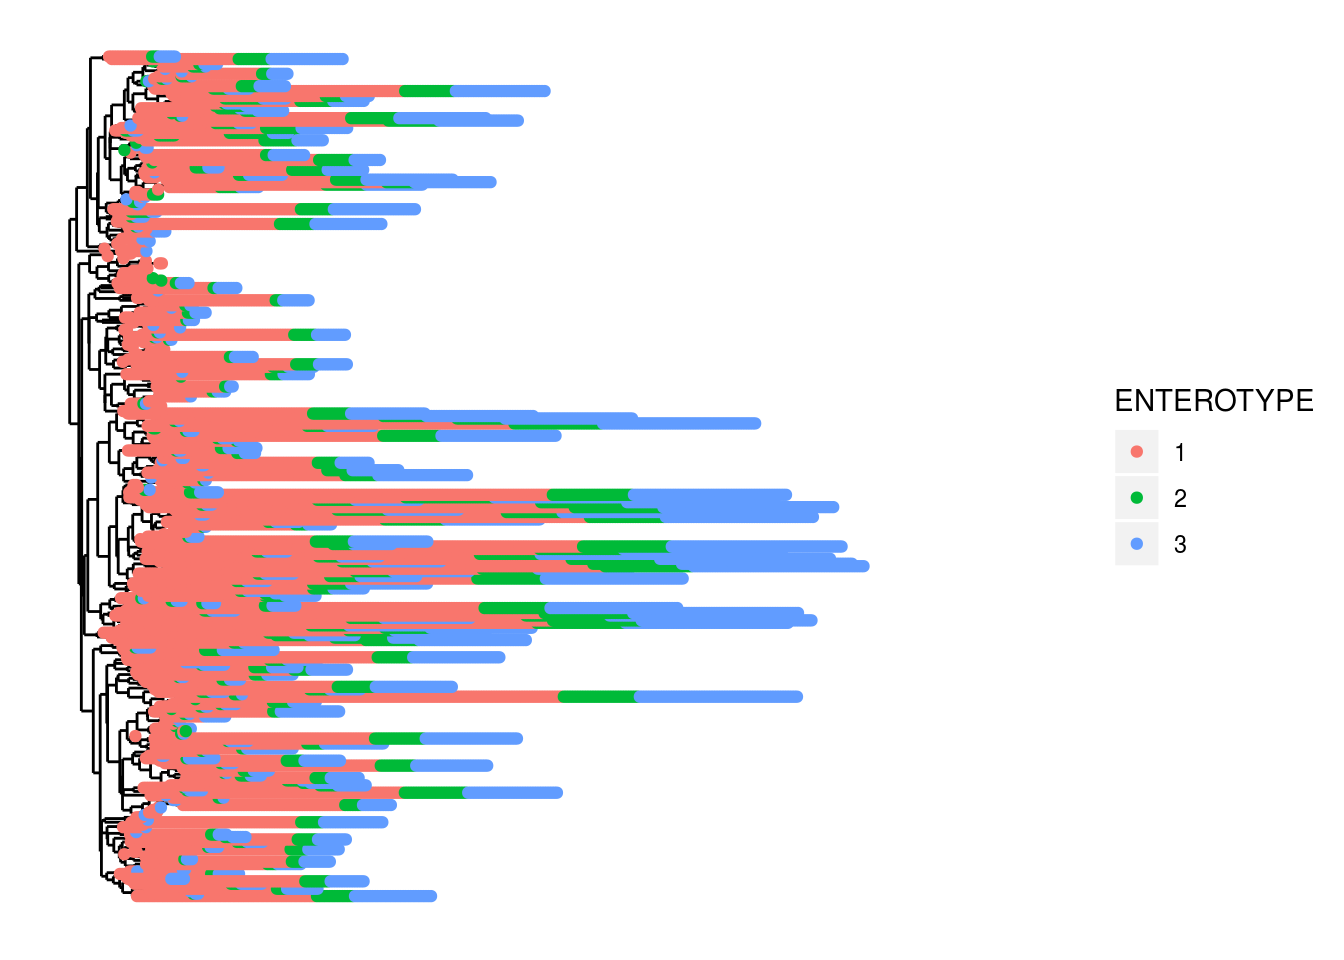
\includegraphics{06_phyloseq_files/figure-latex/unnamed-chunk-10-1.pdf}

\begin{Shaded}
\begin{Highlighting}[]
\KeywordTok{plot_bar}\NormalTok{(PS1,}\DataTypeTok{fill=}\StringTok{'Group'}\NormalTok{)}
\end{Highlighting}
\end{Shaded}

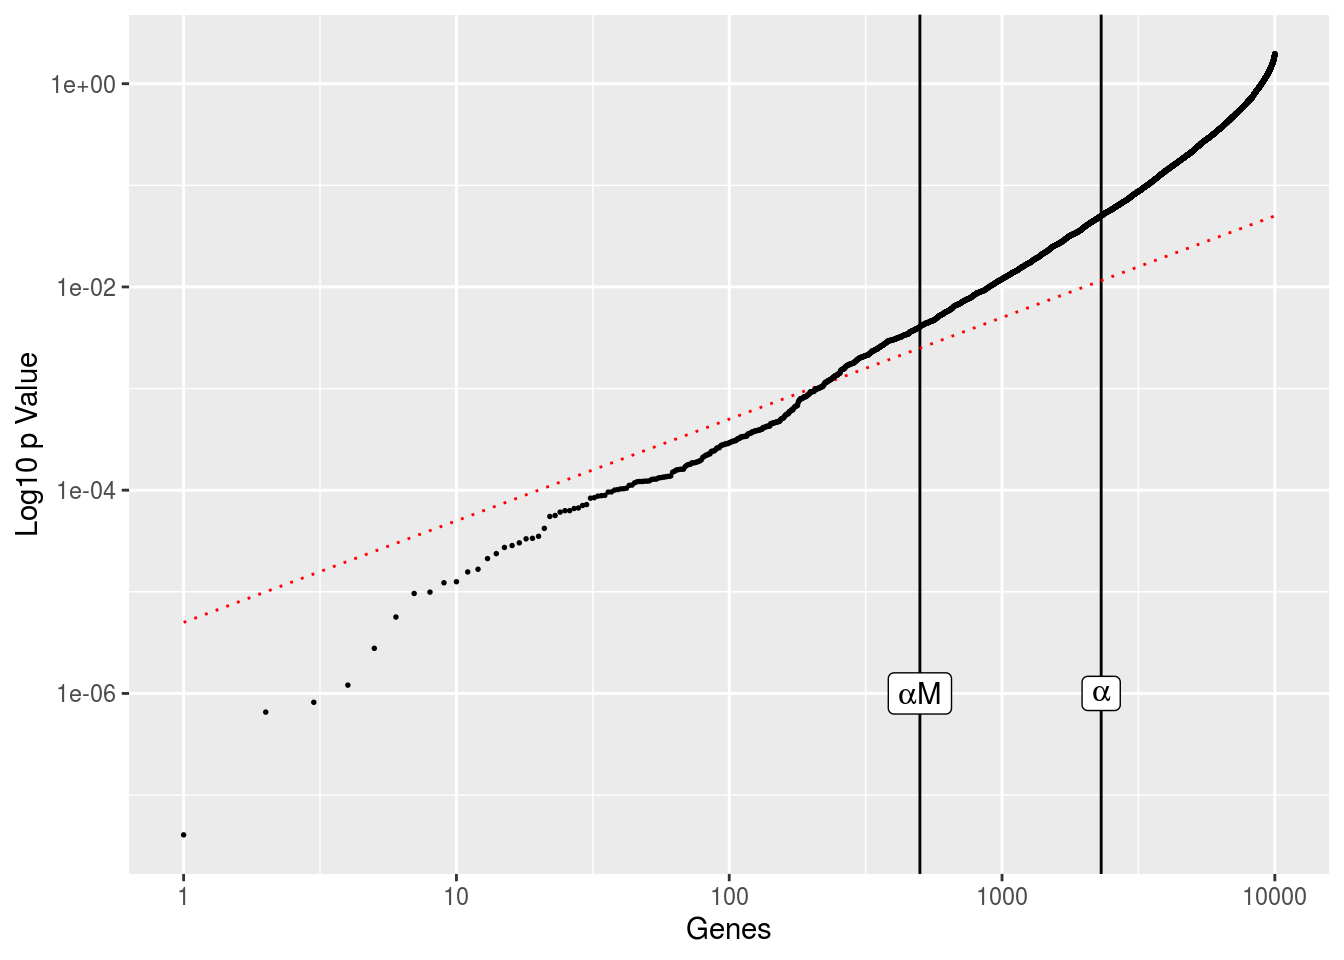
\includegraphics{06_phyloseq_files/figure-latex/unnamed-chunk-11-1.pdf}

And a heatmap, but using subsetted data:

\begin{Shaded}
\begin{Highlighting}[]
\NormalTok{PS2 <-}\StringTok{ }\KeywordTok{prune_taxa}\NormalTok{(}\KeywordTok{names}\NormalTok{(}\KeywordTok{sort}\NormalTok{(}\KeywordTok{taxa_sums}\NormalTok{(PS1),}\DataTypeTok{decreasing=}\OtherTok{TRUE}\NormalTok{))[}\DecValTok{1}\NormalTok{:}\DecValTok{50}\NormalTok{],PS1)}
\KeywordTok{plot_heatmap}\NormalTok{(PS2,}\DataTypeTok{sample.order=}\StringTok{'ENTEROTYPE'}\NormalTok{,}\DataTypeTok{method=}\StringTok{'MDS'}\NormalTok{,}\DataTypeTok{distance=}\StringTok{'bray'}\NormalTok{)}
\end{Highlighting}
\end{Shaded}

\begin{verbatim}
## Warning: Transformation introduced infinite values in discrete y-axis
\end{verbatim}

\includegraphics{06_phyloseq_files/figure-latex/unnamed-chunk-12-1.pdf}

Ordination is quite easy as well.

\begin{Shaded}
\begin{Highlighting}[]
\NormalTok{ORD <-}\StringTok{ }\KeywordTok{ordinate}\NormalTok{(PS1,}\DataTypeTok{method=}\StringTok{'MDS'}\NormalTok{,}\DataTypeTok{distance=}\StringTok{'bray'}\NormalTok{)}
\KeywordTok{plot_ordination}\NormalTok{(PS1,ORD,}\DataTypeTok{color=}\StringTok{'ENTEROTYPE'}\NormalTok{) +}\StringTok{ }\KeywordTok{geom_point}\NormalTok{(}\DataTypeTok{size=}\DecValTok{5}\NormalTok{)}
\end{Highlighting}
\end{Shaded}

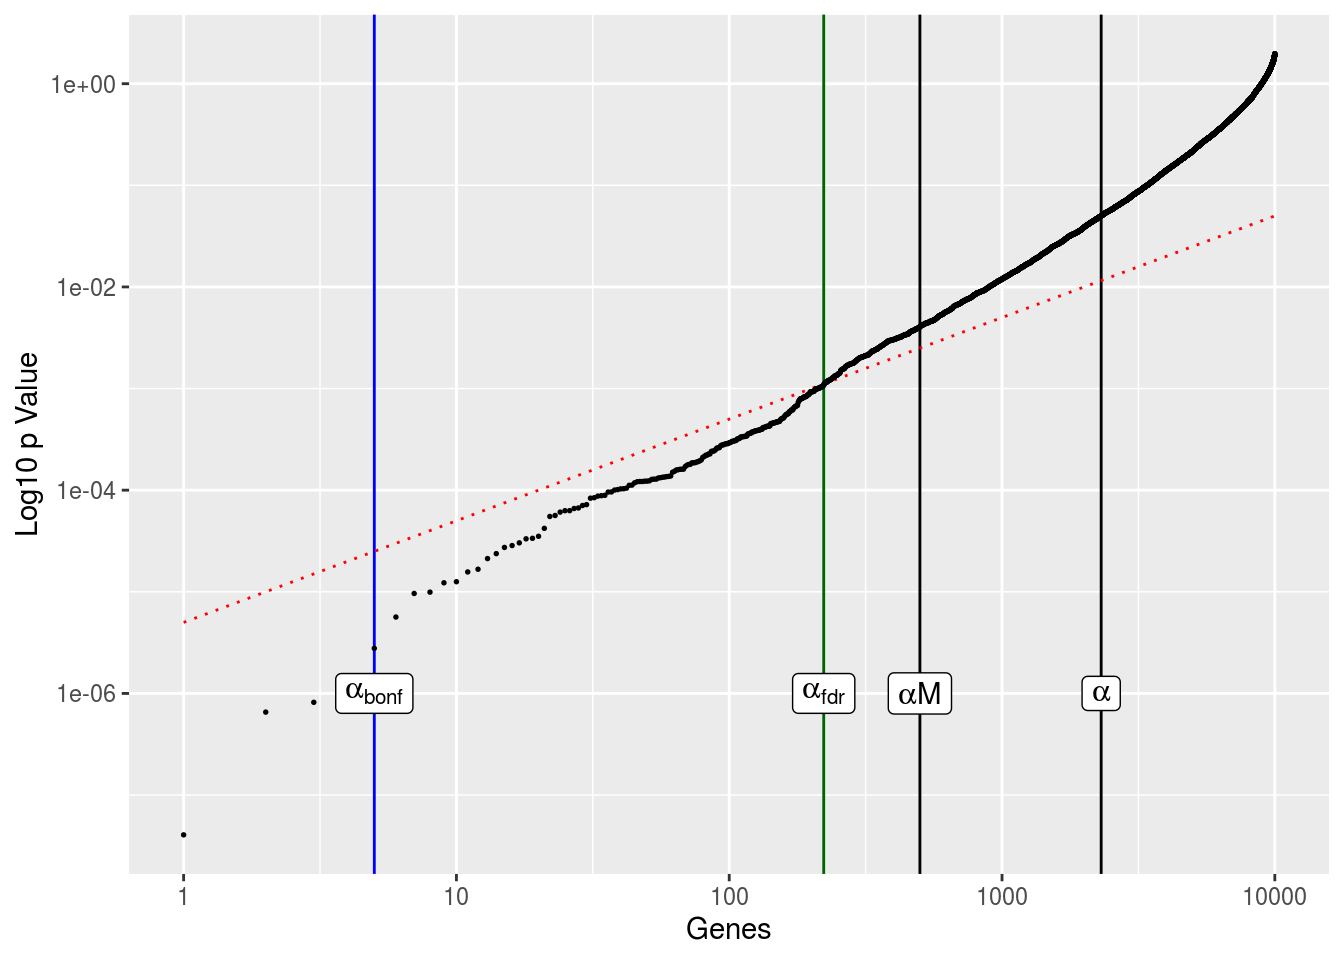
\includegraphics{06_phyloseq_files/figure-latex/unnamed-chunk-13-1.pdf}

And networks

\begin{Shaded}
\begin{Highlighting}[]
\NormalTok{NET <-}\StringTok{ }\KeywordTok{make_network}\NormalTok{(PS1,}\DataTypeTok{max.dist=}\NormalTok{.}\DecValTok{3}\NormalTok{,}\DataTypeTok{distance=}\StringTok{'bray'}\NormalTok{)}
\KeywordTok{plot_network}\NormalTok{(NET,PS1,}\DataTypeTok{color=}\StringTok{'ENTEROTYPE'}\NormalTok{,}\DataTypeTok{label=}\OtherTok{NULL}\NormalTok{)}
\end{Highlighting}
\end{Shaded}

\begin{verbatim}
## Warning: attributes are not identical across measure variables; they will be
## dropped
\end{verbatim}

\includegraphics{06_phyloseq_files/figure-latex/unnamed-chunk-14-1.pdf}

And lastly, let's say we wanted to perform a differential abundance
analysis between genders using DESeq2:

\begin{Shaded}
\begin{Highlighting}[]
\NormalTok{PS3 <-}\StringTok{ }\KeywordTok{prune_samples}\NormalTok{(!}\KeywordTok{is.na}\NormalTok{(}\KeywordTok{sample_data}\NormalTok{(PS)$Gender),PS)}
\NormalTok{PS3 <-}\StringTok{ }\KeywordTok{filter_taxa}\NormalTok{(PS3,function(x) }\KeywordTok{sum}\NormalTok{(x) >}\StringTok{ }\DecValTok{0}\NormalTok{,}\DataTypeTok{prune =} \OtherTok{TRUE}\NormalTok{)}

\NormalTok{diagdds <-}\StringTok{ }\KeywordTok{phyloseq_to_deseq2}\NormalTok{(PS3, ~}\StringTok{ }\NormalTok{Gender)}
\end{Highlighting}
\end{Shaded}

\begin{verbatim}
## converting counts to integer mode
\end{verbatim}

\begin{Shaded}
\begin{Highlighting}[]
\NormalTok{diagdds <-}\StringTok{ }\KeywordTok{DESeq}\NormalTok{(diagdds, }\DataTypeTok{test=}\StringTok{'Wald'}\NormalTok{, }\DataTypeTok{fitType=}\StringTok{'parametric'}\NormalTok{)}
\end{Highlighting}
\end{Shaded}

\begin{verbatim}
## estimating size factors
\end{verbatim}

\begin{verbatim}
## estimating dispersions
\end{verbatim}

\begin{verbatim}
## gene-wise dispersion estimates
\end{verbatim}

\begin{verbatim}
## mean-dispersion relationship
\end{verbatim}

\begin{verbatim}
## final dispersion estimates
\end{verbatim}

\begin{verbatim}
## fitting model and testing
\end{verbatim}

\begin{verbatim}
## -- replacing outliers and refitting for 40 genes
## -- DESeq argument 'minReplicatesForReplace' = 7 
## -- original counts are preserved in counts(dds)
\end{verbatim}

\begin{verbatim}
## estimating dispersions
\end{verbatim}

\begin{verbatim}
## fitting model and testing
\end{verbatim}

\begin{Shaded}
\begin{Highlighting}[]
\NormalTok{res <-}\StringTok{ }\KeywordTok{results}\NormalTok{(diagdds, }\DataTypeTok{cooksCutoff =} \OtherTok{FALSE}\NormalTok{)}
\NormalTok{res}
\end{Highlighting}
\end{Shaded}

\begin{verbatim}
## log2 fold change (MLE): Gender M vs F 
## Wald test p-value: Gender M vs F 
## DataFrame with 135 rows and 6 columns
##                  baseMean      log2FoldChange             lfcSE
##                 <numeric>           <numeric>         <numeric>
## otu1      4828.4506120415   0.245290778934588 0.274237524136042
## otu5    0.408423815044056  -0.763578551311355  1.79402732847231
## otu8   0.0792034228989187 -0.0356169619939926  2.98069121886303
## otu9   0.0320327532464582 -0.0814917834894285  2.98139846283725
## otu29   0.264845130897552   0.300955738130655  1.94223006989263
## ...                   ...                 ...               ...
## otu245   157.499213859763  0.0699225946302586 0.771481998887212
## otu246 0.0555641881033384  0.0556347017417495  2.98128159912465
## otu247   8.66211938696038    0.21953394551718 0.554061558082688
## otu248   5.17914838549527    0.97428692011149 0.580195818970534
## otu249  0.370083654698921  -0.103761272249879  1.25671122049443
##                       stat             pvalue              padj
##                  <numeric>          <numeric>         <numeric>
## otu1     0.894446446405729  0.371083071088348 0.999308335917726
## otu5    -0.425622586229818  0.670382879571334 0.999308335917726
## otu8    -0.011949229013926  0.990466121537832 0.999308335917726
## otu9   -0.0273334089707274  0.978193810311412 0.999308335917726
## otu29    0.154953701312683  0.876857817345056 0.999308335917726
## ...                    ...                ...               ...
## otu245  0.0906341233251264   0.92778331701462 0.999308335917726
## otu246  0.0186613373785572  0.985111271182231 0.999308335917726
## otu247   0.396226632789451  0.691937845592669 0.999308335917726
## otu248    1.67923809213277 0.0931056508804161 0.999308335917726
## otu249 -0.0825657243746543  0.934196856171995 0.999308335917726
\end{verbatim}

\section{Dada2}\label{dada}

\begin{Shaded}
\begin{Highlighting}[]
\KeywordTok{library}\NormalTok{(tidyverse)}
\KeywordTok{library}\NormalTok{(dada2)}
\KeywordTok{library}\NormalTok{(gridExtra)}
\KeywordTok{library}\NormalTok{(DECIPHER)}
\KeywordTok{library}\NormalTok{(ape)}
\KeywordTok{library}\NormalTok{(phangorn)}
\KeywordTok{library}\NormalTok{(phyloseq)}
\end{Highlighting}
\end{Shaded}

First we need to use some qiime functions via the command line, so we'll
save them as variable names.

\begin{Shaded}
\begin{Highlighting}[]
\NormalTok{validate_mapping_file <-}\StringTok{ '/data/sw1/anaconda3/envs/qiime1/bin/validate_mapping_file.py'}
\NormalTok{split_libraries_fastq <-}\StringTok{ '/data/sw1/anaconda3/envs/qiime1/bin/split_libraries_fastq.py'}
\NormalTok{split_sequence_file_on_sample_ids <-}\StringTok{ '/data/sw1/anaconda3/envs/qiime1/bin/split_sequence_file_on_sample_ids.py'}
\end{Highlighting}
\end{Shaded}

\subsection{FASTQ Prep}\label{fastq-prep}

We're going to use the same data as we did with QIIME. Dada2 requires
individual fastq files for each sample, so we'll split our single fastq
file using a few QIIME commands.

\begin{Shaded}
\begin{Highlighting}[]
\NormalTok{data_dir <-}\StringTok{ 'data/data_moving_pictures'}

\NormalTok{MAP <-}\StringTok{ }\KeywordTok{read_delim}\NormalTok{(}\KeywordTok{file.path}\NormalTok{(data_dir,}\StringTok{'map.tsv'}\NormalTok{),}\StringTok{'}\CharTok{\textbackslash{}t}\StringTok{'}\NormalTok{)}
\end{Highlighting}
\end{Shaded}

\begin{verbatim}
## Parsed with column specification:
## cols(
##   `#SampleID` = col_character(),
##   BarcodeSequence = col_character(),
##   LinkerPrimerSequence = col_character(),
##   SampleType = col_character(),
##   Year = col_double(),
##   Month = col_double(),
##   Day = col_double(),
##   Subject = col_double(),
##   ReportedAntibioticUsage = col_character(),
##   DaysSinceExperimentStart = col_double(),
##   Description = col_character()
## )
\end{verbatim}

Note that now we are forcing the split libraries command to also return
a demultiplexed fastq file. We going to also add a bunch of arguments to
ensure that QIIME does \emph{no} filtering. We want to deal with that
using dada2.

\begin{Shaded}
\begin{Highlighting}[]
\KeywordTok{system2}\NormalTok{(split_libraries_fastq,}\DataTypeTok{args=}\KeywordTok{c}\NormalTok{(}\StringTok{'-o'}\NormalTok{,}\KeywordTok{file.path}\NormalTok{(data_dir,}\StringTok{'fastq_out_3'}\NormalTok{),}
                                     \StringTok{'-i'}\NormalTok{,}\KeywordTok{file.path}\NormalTok{(data_dir,}\StringTok{'forward_reads.fastq.gz'}\NormalTok{),}
                                     \StringTok{'-b'}\NormalTok{,}\KeywordTok{file.path}\NormalTok{(data_dir,}\StringTok{'barcodes.fastq.gz'}\NormalTok{),}
                                     \StringTok{'-m'}\NormalTok{,}\KeywordTok{file.path}\NormalTok{(data_dir,}\StringTok{'map.tsv'}\NormalTok{),}
                                     \StringTok{'-r'}\NormalTok{,}\StringTok{'999'}\NormalTok{,}
                                     \StringTok{'-n'}\NormalTok{,}\StringTok{'999'}\NormalTok{,}
                                     \StringTok{'-q'}\NormalTok{,}\StringTok{'0'}\NormalTok{,}
                                     \StringTok{'-p'}\NormalTok{,}\StringTok{'0.0001'}\NormalTok{,}
                                     \StringTok{'--store_demultiplexed_fastq'}\NormalTok{))}
\end{Highlighting}
\end{Shaded}

Next, we'll split these fastq file into separate files for each sample:

\begin{Shaded}
\begin{Highlighting}[]
\KeywordTok{system2}\NormalTok{(split_sequence_file_on_sample_ids,}\DataTypeTok{args=}\KeywordTok{c}\NormalTok{(}\StringTok{'-i'}\NormalTok{,}\KeywordTok{file.path}\NormalTok{(data_dir,}\StringTok{'fastq_out_3'}\NormalTok{,}\StringTok{'seqs.fastq'}\NormalTok{),}
                                                 \StringTok{'-o'}\NormalTok{,}\KeywordTok{file.path}\NormalTok{(data_dir,}\StringTok{'fastq_out_3'}\NormalTok{,}\StringTok{'sequences'}\NormalTok{),}
                                                 \StringTok{'--file_type'}\NormalTok{,}\StringTok{'fastq'}\NormalTok{))}
\end{Highlighting}
\end{Shaded}

\subsection{OTU Picking}\label{otu-picking}

We're now going to run through the dada2 workflow. Dada2 is a
\emph{reference free} method, so this is analogous to de novo OTU
picking had we used QIIME. Still, we can cluster our resulting count
table into OTUs using a reference database; hence, we can compare our
results.

Dada2 captures metagenomic variation by exploiting illumina sequencing
errors. Briefly, everything is based on an error model (a Poisson
distribution). A given read is defined as a \emph{sample} sequence and
is compared to all other reads. The model calculates the probability
these reads were generated from the sample sequence given the error
model -- that is, the probability that these reads resulted from
independent sequencing errors that were generated based on given
transition probabilities and quality scores. If a set of reads are too
abundant to be explained by this error model, then they are separated
into their own partition. The game is to continuously partition the
reads until each partition is consistent with the error model, allowing
us to separate true biological variation from the variation solely due
to sequencing error. At this point, the abundance of reads within a
partition can be calculated, giving us an abundance table. We can then
compare the sequences associated with a given partition to a reference
database to assign taxonomy.

\begin{Shaded}
\begin{Highlighting}[]
\NormalTok{fqs <-}\StringTok{ }\KeywordTok{list.files}\NormalTok{(}\KeywordTok{file.path}\NormalTok{(data_dir,}\StringTok{'fastq_out_3'}\NormalTok{,}\StringTok{'sequences'}\NormalTok{),}\DataTypeTok{full.names=}\OtherTok{TRUE}\NormalTok{)}
\end{Highlighting}
\end{Shaded}

The first thing we'll do is plot the quality scores as a function of
base position. If you recall the definition of Q from the QIIME
tutorial, this should make sense to you, and it should also help you
appriciate setting those parameters for quality filtering before.

\begin{Shaded}
\begin{Highlighting}[]
\NormalTok{sample_idx <-}\StringTok{ }\KeywordTok{sample}\NormalTok{(}\KeywordTok{length}\NormalTok{(fqs),}\DecValTok{5}\NormalTok{)}
\NormalTok{for (i in sample_idx) }\KeywordTok{print}\NormalTok{(}\KeywordTok{plotQualityProfile}\NormalTok{(fqs[i]))}
\end{Highlighting}
\end{Shaded}

\begin{verbatim}
## Scale for 'y' is already present. Adding another scale for 'y', which will
## replace the existing scale.
## Scale for 'y' is already present. Adding another scale for 'y', which will
## replace the existing scale.
\end{verbatim}

\includegraphics{07_dada2_files/figure-latex/unnamed-chunk-8-1.pdf}

\begin{verbatim}
## Scale for 'y' is already present. Adding another scale for 'y', which will
## replace the existing scale.
\end{verbatim}

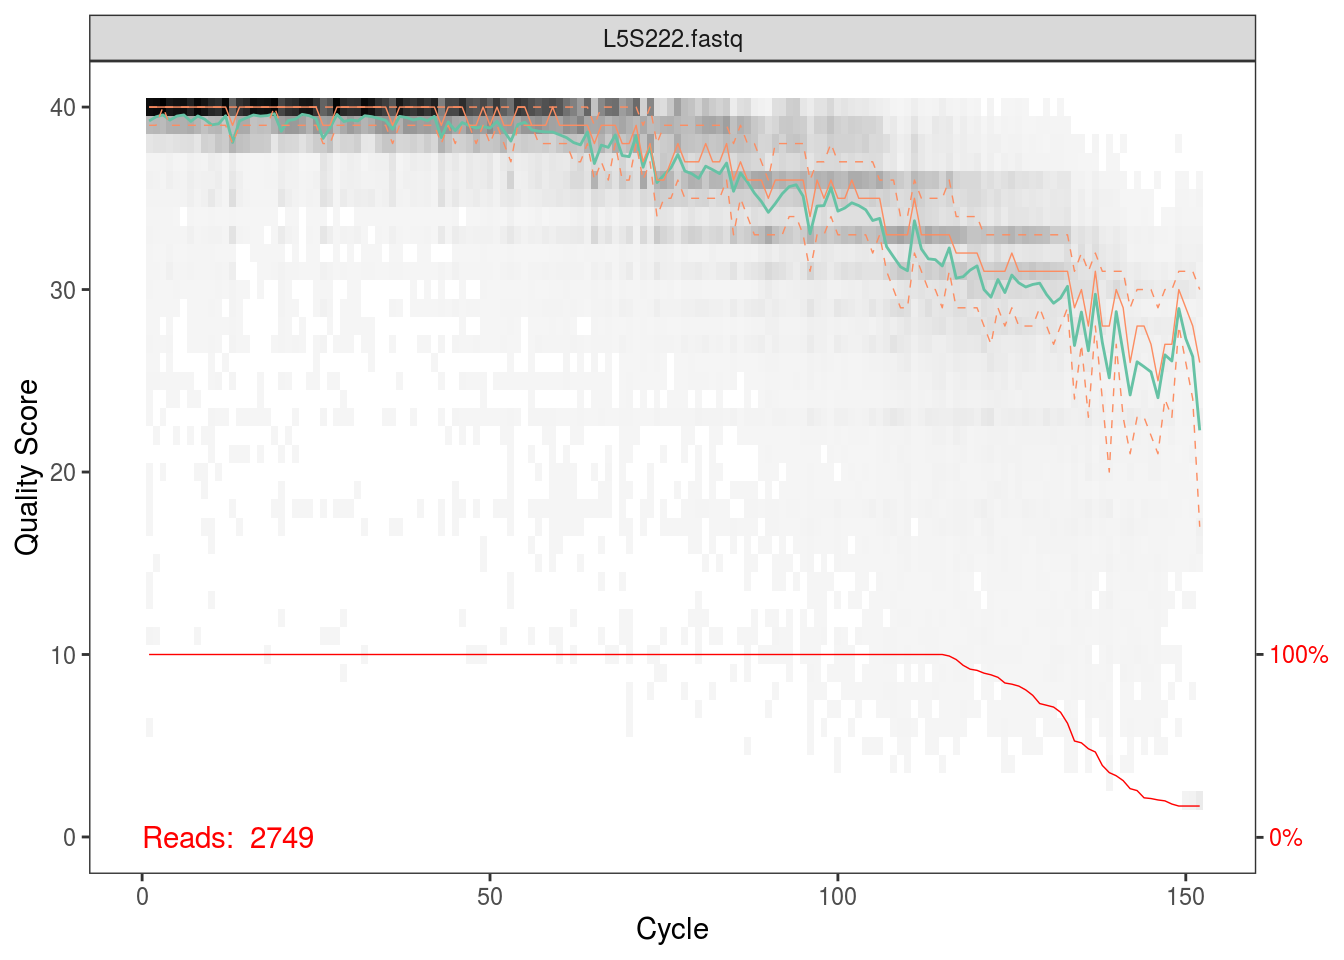
\includegraphics{07_dada2_files/figure-latex/unnamed-chunk-8-2.pdf}

\begin{verbatim}
## Scale for 'y' is already present. Adding another scale for 'y', which will
## replace the existing scale.
\end{verbatim}

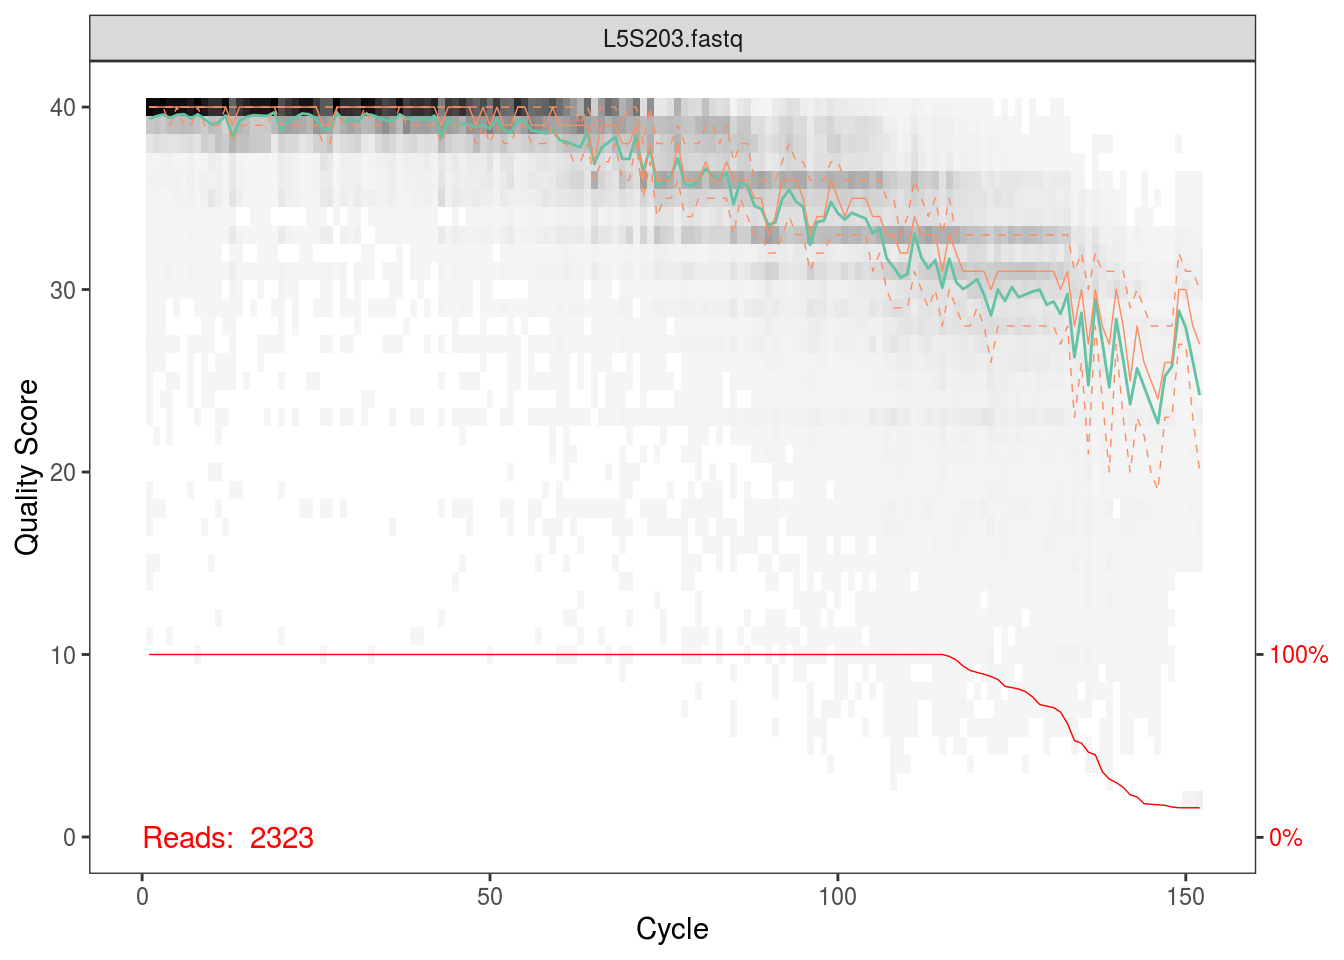
\includegraphics{07_dada2_files/figure-latex/unnamed-chunk-8-3.pdf}

\begin{verbatim}
## Scale for 'y' is already present. Adding another scale for 'y', which will
## replace the existing scale.
\end{verbatim}

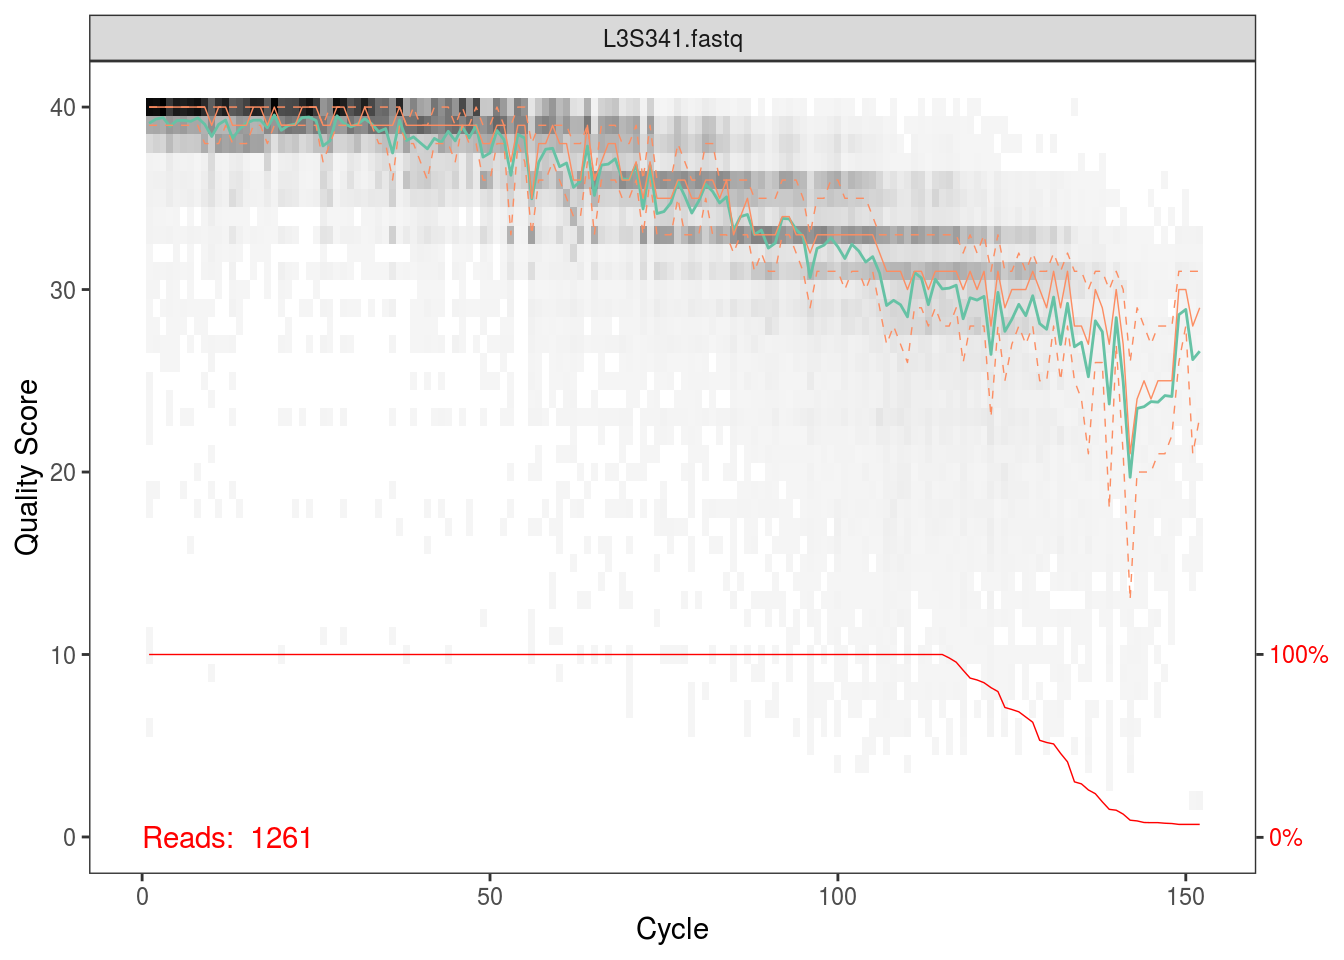
\includegraphics{07_dada2_files/figure-latex/unnamed-chunk-8-4.pdf}
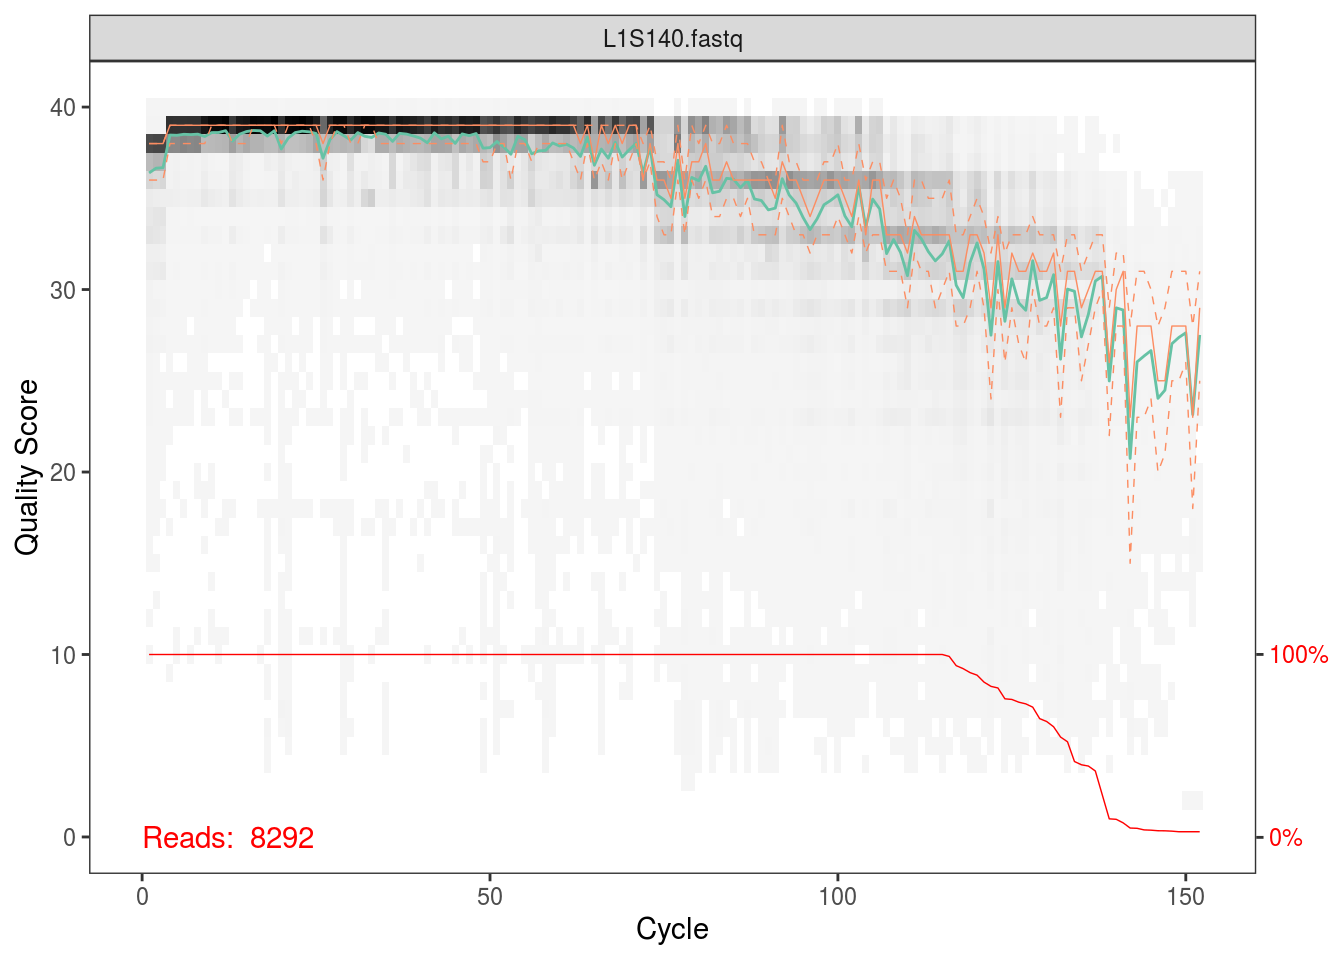
\includegraphics{07_dada2_files/figure-latex/unnamed-chunk-8-5.pdf}

Per the Holmes group, illumina datasets often have errors in the first
10 base positions. Also, given the plots above, there seems to be a drop
in quality towards the end of each read. Hence, we'll trim our reads
such that we keep bases 10 through 130.

\begin{Shaded}
\begin{Highlighting}[]
\NormalTok{fqs_filt <-}\StringTok{ }\KeywordTok{gsub}\NormalTok{(}\StringTok{'sequences'}\NormalTok{,}\StringTok{'filtered'}\NormalTok{,fqs)}
\KeywordTok{dir.create}\NormalTok{(}\KeywordTok{gsub}\NormalTok{(}\StringTok{'(filtered).*'}\NormalTok{,}\StringTok{'}\CharTok{\textbackslash{}\textbackslash{}}\StringTok{1'}\NormalTok{,fqs_filt[}\DecValTok{1}\NormalTok{]),}\DataTypeTok{showWarnings=}\OtherTok{FALSE}\NormalTok{)}
\NormalTok{for (i in }\KeywordTok{seq_along}\NormalTok{(fqs))\{}
  \KeywordTok{fastqFilter}\NormalTok{(fqs[i],fqs_filt[i],}
              \DataTypeTok{trimLeft=}\DecValTok{10}\NormalTok{, }\DataTypeTok{truncLen=}\DecValTok{130}\NormalTok{,}
              \DataTypeTok{maxN=}\DecValTok{0}\NormalTok{, }\DataTypeTok{maxEE=}\DecValTok{2}\NormalTok{, }\DataTypeTok{truncQ=}\DecValTok{2}\NormalTok{,}
              \DataTypeTok{compress=}\OtherTok{TRUE}\NormalTok{)}
\NormalTok{\}}
\end{Highlighting}
\end{Shaded}

The following command performs dereplication, returning a set of unique
sequences and abundances from our set of fastq files.

\begin{Shaded}
\begin{Highlighting}[]
\NormalTok{derep <-}\StringTok{ }\KeywordTok{derepFastq}\NormalTok{(fqs_filt)}
\KeywordTok{names}\NormalTok{(derep) <-}\StringTok{ }\KeywordTok{sapply}\NormalTok{(}\KeywordTok{strsplit}\NormalTok{(}\KeywordTok{basename}\NormalTok{(fqs_filt), }\StringTok{"_"}\NormalTok{), }\StringTok{`}\DataTypeTok{[}\StringTok{`}\NormalTok{, }\DecValTok{1}\NormalTok{)}
\end{Highlighting}
\end{Shaded}

Dada2's error model depends on the fact that there are 16x41 transition
probabilities, but if these values are unknown, we can simply estimate
them from the data. However, estimating the error rates to parameterize
the model is costly, so it's recommended to do this on a subset of the
data, and then use these parameter estimates for the complete dataset:

\begin{Shaded}
\begin{Highlighting}[]
\NormalTok{dd_err <-}\StringTok{ }\KeywordTok{dada}\NormalTok{(derep[}\DecValTok{1}\NormalTok{:}\DecValTok{10}\NormalTok{], }\DataTypeTok{err=}\OtherTok{NULL}\NormalTok{, }\DataTypeTok{selfConsist=}\OtherTok{TRUE}\NormalTok{)}
\end{Highlighting}
\end{Shaded}

\begin{verbatim}
## Initializing error rates to maximum possible estimate.
## selfConsist step 1 ..........
##    selfConsist step 2
##    selfConsist step 3
##    selfConsist step 4
##    selfConsist step 5
##    selfConsist step 6
##    selfConsist step 7
## Convergence after  7  rounds.
\end{verbatim}

We can visualize the error estimates. This shows the frequency of each
base transition as a function of quality score.

\begin{Shaded}
\begin{Highlighting}[]
\KeywordTok{plotErrors}\NormalTok{(dd_err,}\DataTypeTok{err_in=}\OtherTok{TRUE}\NormalTok{,}\DataTypeTok{nominalQ=}\OtherTok{TRUE}\NormalTok{)}
\end{Highlighting}
\end{Shaded}

\begin{verbatim}
## Warning: Transformation introduced infinite values in continuous y-axis

## Warning: Transformation introduced infinite values in continuous y-axis
\end{verbatim}

\includegraphics{07_dada2_files/figure-latex/unnamed-chunk-12-1.pdf}

We'll now fit the full error model, using the estimated error rates from
our subset of data. This step can be parallelized using the multihread
argument. We're also going to pool across samples, since this improves
the detection of variants that are rare in a specific sample but less
rare overall, but at a computational cost.

Note that we can pass a lot of arguments into this function that control
the error model. As briefly described above, the game is to partition
these sequences until each partition is consistent with being generated
soley by illumina and amplification error variation, and not due to
biological variation. A p-value is calculated to test the sequences that
form new partitions, with signififcant p-values at a given threshold
leading to new parittions.

Now, say we had a problem where rare sequence variants were of most
interest. It would then make sense to use a less conservative
significance threshold, leading to \emph{more} significant p-values,
more partitions, and hence more rare variants. We can do this by
increasing the \textbf{OMEGA\_A} value from its default value of
\(1\times10^{-40}\). We'll fit a second model and change the threshold
to \(1\times10^{-20}\).

\begin{Shaded}
\begin{Highlighting}[]
\NormalTok{dd <-}\StringTok{ }\KeywordTok{dada}\NormalTok{(derep, }\DataTypeTok{err=}\NormalTok{dd_err[[}\DecValTok{1}\NormalTok{]]$err_out, }\DataTypeTok{pool=}\OtherTok{TRUE}\NormalTok{)}
\end{Highlighting}
\end{Shaded}

\begin{verbatim}
## 34 samples were pooled: 109854 reads in 18034 unique sequences.
\end{verbatim}

\begin{Shaded}
\begin{Highlighting}[]
\NormalTok{dd_rare <-}\StringTok{ }\KeywordTok{dada}\NormalTok{(derep, }\DataTypeTok{err=}\NormalTok{dd_err[[}\DecValTok{1}\NormalTok{]]$err_out, }\DataTypeTok{pool=}\OtherTok{TRUE}\NormalTok{, }\DataTypeTok{OMEGA_A=}\FloatTok{1e-20}\NormalTok{)}
\end{Highlighting}
\end{Shaded}

\begin{verbatim}
## 34 samples were pooled: 109854 reads in 18034 unique sequences.
\end{verbatim}

Finally, we'll make our sequence table.

\begin{Shaded}
\begin{Highlighting}[]
\NormalTok{seqtab_all <-}\StringTok{ }\KeywordTok{makeSequenceTable}\NormalTok{(dd)}
\NormalTok{seqtab_all_rare <-}\StringTok{ }\KeywordTok{makeSequenceTable}\NormalTok{(dd_rare)}
\end{Highlighting}
\end{Shaded}

And then we'll remove chimeras. This function compares sequences against
one another, and removes sequences that can be generated by joining two
abundant sequences.

\begin{Shaded}
\begin{Highlighting}[]
\NormalTok{seqtab <-}\StringTok{ }\KeywordTok{removeBimeraDenovo}\NormalTok{(seqtab_all)}
\NormalTok{seqtab_rare <-}\StringTok{ }\KeywordTok{removeBimeraDenovo}\NormalTok{(seqtab_all_rare)}
\end{Highlighting}
\end{Shaded}

First, note the difference in dimensions; there are more sequences in
the rare table:

\begin{Shaded}
\begin{Highlighting}[]
\KeywordTok{ncol}\NormalTok{(seqtab)}
\end{Highlighting}
\end{Shaded}

\begin{verbatim}
## [1] 662
\end{verbatim}

\begin{Shaded}
\begin{Highlighting}[]
\KeywordTok{ncol}\NormalTok{(seqtab_rare)}
\end{Highlighting}
\end{Shaded}

\begin{verbatim}
## [1] 817
\end{verbatim}

Also note that despite now having a sequence abundance table that is
similar in form to the OTU table we generated in QIIME, our `taxonomic
variants' are unique sequences and \emph{not} OTUs:

\begin{Shaded}
\begin{Highlighting}[]
\NormalTok{seqtab[}\DecValTok{1}\NormalTok{:}\DecValTok{5}\NormalTok{,}\DecValTok{1}\NormalTok{:}\DecValTok{5}\NormalTok{]}
\end{Highlighting}
\end{Shaded}

\begin{verbatim}
##              CCGAGCGTTATCCGGATTTATTGGGTTTAAAGGGAGCGTAGATGGATGTTTAAGTCAGTTGTGAAAGTTTGCGGCTCAACCGTAAAATTGCAGTTGATACTGGATATCTTGAGTGCAGTT
## L1S105.fastq                                                                                                                     1769
## L1S140.fastq                                                                                                                        8
## L1S208.fastq                                                                                                                       11
## L1S257.fastq                                                                                                                        6
## L1S281.fastq                                                                                                                        4
##              GCGAGCGTTAATCGGAATTACTGGGCGTAAAGCGAGCGCAGACGGTTACTTAAGCAGGATGTGAAATCCCCGGGCTCAACCTGGGAACTGCGTTCTGAACTGGGTGACTAGAGTGTGTCA
## L1S105.fastq                                                                                                                        5
## L1S140.fastq                                                                                                                        1
## L1S208.fastq                                                                                                                        0
## L1S257.fastq                                                                                                                        0
## L1S281.fastq                                                                                                                        0
##              CCGAGCGTTATCCGGATTTATTGGGTTTAAAGGGAGCGTAGATGGATGTTTAAGTCAGTTGTGAAAGTTTGCGGCTCAACCGTAAAATTGCAGTTGATACTGGATGTCTTGAGTGCAGTT
## L1S105.fastq                                                                                                                        8
## L1S140.fastq                                                                                                                     1531
## L1S208.fastq                                                                                                                     1552
## L1S257.fastq                                                                                                                      870
## L1S281.fastq                                                                                                                     1196
##              GCGAGCGTTAATCGGAATAACTGGGCGTAAAGGGCACGCAGGCGGTGACTTAAGTGAGGTGTGAAAGCCCCGGGCTTAACCTGGGAATTGCATTTCATACTGGGTCGCTAGAGTACTTTA
## L1S105.fastq                                                                                                                        0
## L1S140.fastq                                                                                                                        0
## L1S208.fastq                                                                                                                        5
## L1S257.fastq                                                                                                                        0
## L1S281.fastq                                                                                                                        0
##              CCGAGCGTTGTCCGGATTTATTGGGCGTAAAGCGAGCGCAGGCGGTTAGATAAGTCTGAAGTTAAAGGCTGTGGCTTAACCATAGTACGCTTTGGAAACTGTTTAACTTGAGTGCAAGAG
## L1S105.fastq                                                                                                                        1
## L1S140.fastq                                                                                                                        0
## L1S208.fastq                                                                                                                        2
## L1S257.fastq                                                                                                                        0
## L1S281.fastq                                                                                                                        0
\end{verbatim}

If we want to assign taxonomy from a reference database to these
sequences, we can use the following command that applies a naive Bayes
classifer to compare our sequences to classified sequences in a training
set. First, we'll use a GreenGenes training set:

\begin{Shaded}
\begin{Highlighting}[]
\NormalTok{ref_fasta <-}\StringTok{ 'data/data_stability/references/gg_13_8_train_set_97.fa.gz'}
\NormalTok{taxtab_gg <-}\StringTok{ }\KeywordTok{assignTaxonomy}\NormalTok{(seqtab, }\DataTypeTok{refFasta=}\NormalTok{ref_fasta)}
\KeywordTok{colnames}\NormalTok{(taxtab_gg) <-}\StringTok{ }\KeywordTok{c}\NormalTok{(}\StringTok{"Kingdom"}\NormalTok{, }\StringTok{"Phylum"}\NormalTok{, }\StringTok{"Class"}\NormalTok{, }\StringTok{"Order"}\NormalTok{, }\StringTok{"Family"}\NormalTok{, }\StringTok{"Genus"}\NormalTok{, }\StringTok{"Species"}\NormalTok{)}
\end{Highlighting}
\end{Shaded}

Now, instead, we can try a Silva training set. Note that Silva does not
give species level assignments

\begin{Shaded}
\begin{Highlighting}[]
\NormalTok{ref_fasta <-}\StringTok{ 'data/data_stability/references/silva_nr_v123_train_set.fa.gz'}
\NormalTok{taxtab_silva <-}\StringTok{ }\KeywordTok{assignTaxonomy}\NormalTok{(seqtab, }\DataTypeTok{refFasta=}\NormalTok{ref_fasta)}
\KeywordTok{colnames}\NormalTok{(taxtab_silva) <-}\StringTok{ }\KeywordTok{c}\NormalTok{(}\StringTok{"Kingdom"}\NormalTok{, }\StringTok{"Phylum"}\NormalTok{, }\StringTok{"Class"}\NormalTok{, }\StringTok{"Order"}\NormalTok{, }\StringTok{"Family"}\NormalTok{, }\StringTok{"Genus"}\NormalTok{)}
\end{Highlighting}
\end{Shaded}

If we want species level assignments, we can do the following.

\begin{Shaded}
\begin{Highlighting}[]
\NormalTok{ref_fasta <-}\StringTok{ 'data/data_stability/references/rdp_species_assignment_14.fa.gz'}
\NormalTok{sptab_silva <-}\StringTok{ }\KeywordTok{assignSpecies}\NormalTok{(seqtab, }\DataTypeTok{refFasta=}\NormalTok{ref_fasta, }\DataTypeTok{allowMultiple=}\OtherTok{FALSE}\NormalTok{, }\DataTypeTok{verbose=}\OtherTok{TRUE}\NormalTok{)}
\end{Highlighting}
\end{Shaded}

Next, we might want to build a phylogenetic tree. First, we perform a
multiple sequence alignment:

\begin{Shaded}
\begin{Highlighting}[]
\NormalTok{seqs <-}\StringTok{ }\KeywordTok{getSequences}\NormalTok{(seqtab)}
\KeywordTok{names}\NormalTok{(seqs) <-}\StringTok{ }\NormalTok{seqs}
\NormalTok{alignment <-}\StringTok{ }\KeywordTok{AlignSeqs}\NormalTok{(}\KeywordTok{DNAStringSet}\NormalTok{(seqs), }\DataTypeTok{anchor=}\OtherTok{NA}\NormalTok{)}
\end{Highlighting}
\end{Shaded}

Then, we'll build a tree, specifically, a maximum likelihood tree from a
NJ tree.

\begin{Shaded}
\begin{Highlighting}[]
\NormalTok{phang_align <-}\StringTok{ }\KeywordTok{phyDat}\NormalTok{(}\KeywordTok{as.matrix}\NormalTok{(alignment), }\DataTypeTok{type=}\StringTok{"DNA"}\NormalTok{)}
\NormalTok{dm <-}\StringTok{ }\KeywordTok{dist.ml}\NormalTok{(phang_align)}
\NormalTok{treeNJ <-}\StringTok{ }\KeywordTok{NJ}\NormalTok{(dm) }\CommentTok{# Note, tip order != sequence order}
\NormalTok{fit =}\StringTok{ }\KeywordTok{pml}\NormalTok{(treeNJ, }\DataTypeTok{data=}\NormalTok{phang_align)}

\NormalTok{fit_gtr <-}\StringTok{ }\KeywordTok{update}\NormalTok{(fit, }\DataTypeTok{k=}\DecValTok{4}\NormalTok{, }\DataTypeTok{inv=}\FloatTok{0.2}\NormalTok{)}
\NormalTok{fit_gtr <-}\StringTok{ }\KeywordTok{optim.pml}\NormalTok{(fit_gtr, }\DataTypeTok{model=}\StringTok{"GTR"}\NormalTok{, }\DataTypeTok{optInv=}\OtherTok{TRUE}\NormalTok{, }\DataTypeTok{optGamma=}\OtherTok{TRUE}\NormalTok{,}
                      \DataTypeTok{rearrangement =} \StringTok{"stochastic"}\NormalTok{, }\DataTypeTok{control =} \KeywordTok{pml.control}\NormalTok{(}\DataTypeTok{trace =} \DecValTok{0}\NormalTok{))}
\end{Highlighting}
\end{Shaded}

And finally, we can build our phyloseq object for our GreenGenes table:

\begin{Shaded}
\begin{Highlighting}[]
\NormalTok{TREE <-}\StringTok{ }\KeywordTok{phy_tree}\NormalTok{(fit_gtr)}

\NormalTok{META <-}\StringTok{ }\KeywordTok{as.data.frame}\NormalTok{(MAP)}
\KeywordTok{rownames}\NormalTok{(META) <-}\StringTok{ }\NormalTok{META$}\StringTok{`}\DataTypeTok{#SampleID}\StringTok{`}

\NormalTok{OTU <-}\StringTok{ }\NormalTok{seqtab}
\KeywordTok{rownames}\NormalTok{(OTU) <-}\StringTok{ }\KeywordTok{gsub}\NormalTok{(}\StringTok{'}\CharTok{\textbackslash{}\textbackslash{}}\StringTok{.fastq'}\NormalTok{,}\StringTok{''}\NormalTok{,}\KeywordTok{rownames}\NormalTok{(OTU))}
\NormalTok{OTU <-}\StringTok{ }\NormalTok{OTU[}\KeywordTok{rownames}\NormalTok{(META),]}
\NormalTok{OTU <-}\StringTok{ }\KeywordTok{otu_table}\NormalTok{(OTU,}\DataTypeTok{taxa_are_rows=}\OtherTok{FALSE}\NormalTok{)}
  
\NormalTok{META <-}\StringTok{ }\KeywordTok{sample_data}\NormalTok{(META)}

\NormalTok{TAXA <-}\StringTok{ }\NormalTok{taxtab_gg[}\KeywordTok{colnames}\NormalTok{(OTU),]}
\NormalTok{TAXA <-}\StringTok{ }\KeywordTok{tax_table}\NormalTok{(TAXA)}

\NormalTok{PS <-}\StringTok{ }\KeywordTok{phyloseq}\NormalTok{(OTU,TAXA,META,TREE)}
\end{Highlighting}
\end{Shaded}

\subsection{Running Dada2 on Proteus}\label{running-dada2-on-proteus}

Now let's redo the analysis above, but on a cluster. I'll explain below
how to run dada2 via two ways. The first will involve simply using
packages installed in a shared group folder. The second will cover
installing dada2 in a local folder. If you lack access to the shared
folder, or, if for some reason it no longer exists, go to method 2.

\subsubsection{Method 1: Using nameGrp Shared R
Library}\label{method-1-using-namegrp-shared-r-library}

First, we'll create a bash script that runs some QIIME commands to do
the demultiplexing and splitting, and then runs the dada anlysis. We'll
assume that the moving pictures data is in your home directory. As
before, the folder should contain three files: (1) the reads, (2) the
barcodes, and (3) the mapping file.

We'll name the script \textbf{prep\_sub.sh}:

\begin{Shaded}
\begin{Highlighting}[]
\CommentTok{#!/bin/bash}
\CommentTok{#$ -S /bin/bash}
\CommentTok{#$ -cwd}
\CommentTok{#$ -j y}
\CommentTok{#$ -M user_name@email.edu}
\CommentTok{#$ -l h_rt=01:00:00}
\CommentTok{#$ -P namePrj}
\CommentTok{#$ -l mem_free=12G}
\CommentTok{#$ -l h_vmem=16G}
\CommentTok{#$ -q all.q}

\NormalTok{. /etc/profile.d/modules.sh}
\NormalTok{module load shared}
\NormalTok{module load proteus}
\NormalTok{module load sge/univa}
\NormalTok{module load gcc/}\FloatTok{4.8.1}
\NormalTok{module load qiime/gcc/}\DecValTok{64}\NormalTok{/}\FloatTok{1.9.1}

\NormalTok{export ref_seqs=}\ErrorTok{/}\NormalTok{mnt/HA/opt/qiime/gcc/}\DecValTok{64}\NormalTok{/}\FloatTok{1.9.1}\NormalTok{/lib/python2}\FloatTok{.7}\NormalTok{/site-packages/qiime_default_reference/gg_13_8_otus/rep_set/97_otus.fasta}
\NormalTok{export ref_tax=}\ErrorTok{/}\NormalTok{mnt/HA/opt/qiime/gcc/}\DecValTok{64}\NormalTok{/}\FloatTok{1.9.1}\NormalTok{/lib/python2}\FloatTok{.7}\NormalTok{/site-packages/qiime_default_reference/gg_13_8_otus/taxonomy/97_otu_taxonomy.txt}

\NormalTok{data_dir=}\ErrorTok{/}\NormalTok{home/user_name/dirname/dada2/moving_pictures}
\NormalTok{work_dir=}\ErrorTok{/}\NormalTok{scratch/user_name/moving_pictures}

\NormalTok{mkdir -p $work_dir}

\NormalTok{cp $data_dir/}\ErrorTok{*}\StringTok{ }\ErrorTok{$}\NormalTok{work_dir}

\NormalTok{out_dir=}\ErrorTok{$}\NormalTok{work_dir/fastq_out}
\NormalTok{seqs=}\ErrorTok{$}\NormalTok{work_dir/forward_reads.fastq.gz}
\NormalTok{bc=}\ErrorTok{$}\NormalTok{work_dir/barcodes.fastq.gz}
\NormalTok{map=}\ErrorTok{$}\NormalTok{work_dir/map.tsv}

\NormalTok{split_libraries_fastq.py -o $out_dir -i $seqs -b $bc -m $map -r }\DecValTok{999} \NormalTok{-n }\DecValTok{999} \NormalTok{-q }\DecValTok{0} \NormalTok{-p }\FloatTok{0.0001} \NormalTok{--store_demultiplexed_fastq}
\NormalTok{split_sequence_file_on_sample_ids.py -i $out_dir/seqs.fastq -o $out_dir/sequences --file_type fastq}

\NormalTok{mv $out_dir/sequences $data_dir}
\NormalTok{rm -r $work_dir/}\ErrorTok{*}
\StringTok{  }
\NormalTok{exit }\DecValTok{0}
\end{Highlighting}
\end{Shaded}

This gives us our demultiplexed, split sequences. Now, we'll make a
dada2 R script that performs the actual analysis. We'll call this
\textbf{dada.R}.

\begin{Shaded}
\begin{Highlighting}[]
\KeywordTok{require}\NormalTok{(dada2)}

\NormalTok{scratch_path <-}\StringTok{ '/scratch/user_name/moving_pictures'}
\NormalTok{ref_fasta <-}\StringTok{ }\KeywordTok{file.path}\NormalTok{(scratch_path,}\StringTok{'silva_nr_v123_train_set.fa.gz'}\NormalTok{)}
\NormalTok{fq_dir <-}\StringTok{ }\KeywordTok{file.path}\NormalTok{(scratch_path,}\StringTok{'sequences'}\NormalTok{)}
\NormalTok{fqs <-}\StringTok{ }\KeywordTok{list.files}\NormalTok{(fq_dir,}\DataTypeTok{full.names=}\OtherTok{TRUE}\NormalTok{)}

\NormalTok{fqs_filt <-}\StringTok{ }\KeywordTok{gsub}\NormalTok{(}\StringTok{'sequences'}\NormalTok{,}\StringTok{'filtered'}\NormalTok{,fqs)}
\KeywordTok{dir.create}\NormalTok{(}\KeywordTok{gsub}\NormalTok{(}\StringTok{'(filtered).*'}\NormalTok{,}\StringTok{'}\CharTok{\textbackslash{}\textbackslash{}}\StringTok{1'}\NormalTok{,fqs_filt[}\DecValTok{1}\NormalTok{]),}\DataTypeTok{showWarnings=}\OtherTok{FALSE}\NormalTok{)}
\NormalTok{for (i in }\KeywordTok{seq_along}\NormalTok{(fqs))\{}
  \KeywordTok{fastqFilter}\NormalTok{(fqs[i],fqs_filt[i],}
              \DataTypeTok{trimLeft=}\DecValTok{10}\NormalTok{, }\DataTypeTok{truncLen=}\DecValTok{130}\NormalTok{,}
              \DataTypeTok{maxN=}\DecValTok{0}\NormalTok{, }\DataTypeTok{maxEE=}\DecValTok{2}\NormalTok{, }\DataTypeTok{truncQ=}\DecValTok{2}\NormalTok{,}
              \DataTypeTok{compress=}\OtherTok{TRUE}\NormalTok{)}
\NormalTok{\}}

\NormalTok{derep <-}\StringTok{ }\KeywordTok{derepFastq}\NormalTok{(fqs_filt)}
\KeywordTok{names}\NormalTok{(derep) <-}\StringTok{ }\KeywordTok{sapply}\NormalTok{(}\KeywordTok{strsplit}\NormalTok{(}\KeywordTok{basename}\NormalTok{(fqs_filt), }\StringTok{"_"}\NormalTok{), }\StringTok{`}\DataTypeTok{[}\StringTok{`}\NormalTok{, }\DecValTok{1}\NormalTok{)}

\NormalTok{dd_err <-}\StringTok{ }\KeywordTok{dada}\NormalTok{(derep[}\DecValTok{1}\NormalTok{:}\DecValTok{10}\NormalTok{],}\DataTypeTok{err=}\OtherTok{NULL}\NormalTok{,}\DataTypeTok{selfConsist=}\OtherTok{TRUE}\NormalTok{, }\DataTypeTok{multithread=}\OtherTok{TRUE}\NormalTok{,}\DataTypeTok{VERBOSE=}\OtherTok{TRUE}\NormalTok{)}

\NormalTok{dd <-}\StringTok{ }\KeywordTok{dada}\NormalTok{(derep, }\DataTypeTok{err=}\NormalTok{dd_err[[}\DecValTok{1}\NormalTok{]]$err_out, }\DataTypeTok{pool=}\OtherTok{TRUE}\NormalTok{, }\DataTypeTok{multithread=}\OtherTok{TRUE}\NormalTok{,}\DataTypeTok{VERBOSE=}\OtherTok{TRUE}\NormalTok{)}

\NormalTok{seqtab_all <-}\StringTok{ }\KeywordTok{makeSequenceTable}\NormalTok{(dd)}

\NormalTok{seqtab <-}\StringTok{ }\KeywordTok{removeBimeraDenovo}\NormalTok{(seqtab_all,}\DataTypeTok{tableMethod=}\StringTok{'pooled'}\NormalTok{,}\DataTypeTok{verbose=}\OtherTok{TRUE}\NormalTok{, }\DataTypeTok{multithread=}\OtherTok{TRUE}\NormalTok{)}

\NormalTok{taxtab_silva <-}\StringTok{ }\KeywordTok{assignTaxonomy}\NormalTok{(seqtab,}\DataTypeTok{refFasta=}\NormalTok{ref_fasta,}\DataTypeTok{verbose=}\OtherTok{TRUE}\NormalTok{)}
\KeywordTok{colnames}\NormalTok{(taxtab_silva) <-}\StringTok{ }\KeywordTok{c}\NormalTok{(}\StringTok{"Kingdom"}\NormalTok{, }\StringTok{"Phylum"}\NormalTok{, }\StringTok{"Class"}\NormalTok{, }\StringTok{"Order"}\NormalTok{, }\StringTok{"Family"}\NormalTok{, }\StringTok{"Genus"}\NormalTok{)}

\KeywordTok{saveRDS}\NormalTok{(seqtab,}\KeywordTok{file.path}\NormalTok{(scratch_path,}\StringTok{'seqtab.rds'}\NormalTok{))}
\KeywordTok{saveRDS}\NormalTok{(taxtab_silva,}\KeywordTok{file.path}\NormalTok{(scratch_path,}\StringTok{'taxtab.rds'}\NormalTok{))}
\end{Highlighting}
\end{Shaded}

Finally, we'll create the submission script. \textbf{Note the following
change that allows you to use the packages in the shared folder.} In
this submission script, immediately after you load your modules, you
must add the line:

\begin{Shaded}
\begin{Highlighting}[]
\NormalTok{export R_LIBS=}\ErrorTok{/}\NormalTok{mnt/HA/groups/nameGrp/r_libs}
\end{Highlighting}
\end{Shaded}

This gives us the following submission script:

\begin{Shaded}
\begin{Highlighting}[]
\CommentTok{#!/bin/bash}
\CommentTok{#$ -S /bin/bash}
\CommentTok{#$ -cwd}
\CommentTok{#$ -j y}
\CommentTok{#$ -M user_name@email.edu}
\CommentTok{#$ -l h_rt=01:00:00}
\CommentTok{#$ -P namePrj}
\CommentTok{#$ -pe shm 16}
\CommentTok{#$ -l mem_free=12G}
\CommentTok{#$ -l h_vmem=16G}
\CommentTok{#$ -q all.q}

\NormalTok{. /etc/profile.d/modules.sh}
\NormalTok{module load shared}
\NormalTok{module load proteus}
\NormalTok{module load sge/univa}
\NormalTok{module load gcc/}\FloatTok{4.8.1}

\NormalTok{export R_LIBS=}\ErrorTok{/}\NormalTok{mnt/HA/groups/nameGrp/r_libs}

\NormalTok{data_dir=}\ErrorTok{/}\NormalTok{home/user_name/dirname/dada2}
\NormalTok{work_dir=}\ErrorTok{/}\NormalTok{scratch/user_name/moving_pictures}

\NormalTok{mkdir -p $work_dir}

\NormalTok{cp -r $data_dir/moving_pictures/sequences $work_dir}
\NormalTok{cp $data_dir/dada.R $work_dir}
\NormalTok{cp ~}\ErrorTok{/}\NormalTok{references/silva_nr_v123_train_set.fa.gz $work_dir}

\NormalTok{R CMD BATCH $work_dir/dada.R}

\NormalTok{mv $work_dir/}\ErrorTok{*}\NormalTok{.Rout $data_dir}
\NormalTok{mv $work_dir/}\ErrorTok{*}\NormalTok{.rds $data_dir}
\NormalTok{rm -rf $work_dir}

\NormalTok{exit }\DecValTok{0}
\end{Highlighting}
\end{Shaded}

\subsubsection{Method 2: Creating a Local
Library}\label{method-2-creating-a-local-library}

We first need to make two scripts. One will be an R package script that
installs our packages into a personal library folder. The other will run
this script, but it will first make said folder and also unload any
preloaded gcc modules that may cause conflicts during pacakge
installation.

First, make sure you're in your home directory. We'll now make the R
package installer script. We'll call it \textbf{install\_r\_pkgs.R}.

\begin{Shaded}
\begin{Highlighting}[]
\NormalTok{MYLIB <-}\StringTok{ }\KeywordTok{Sys.getenv}\NormalTok{(}\StringTok{'R_LIBS_USER'}\NormalTok{)}

\KeywordTok{source}\NormalTok{(}\StringTok{'https://bioconductor.org/biocLite.R'}\NormalTok{)}
\KeywordTok{biocLite}\NormalTok{(}\StringTok{'dada2'}\NormalTok{,}\DataTypeTok{lib=}\NormalTok{MYLIB)}
\end{Highlighting}
\end{Shaded}

Next, we'll make the bash script that runs this, which we'll call
\textbf{run\_install\_r\_pkgs.sh}:

\begin{Shaded}
\begin{Highlighting}[]
\CommentTok{#!/bin/bash}

\NormalTok{module unload gcc}

\NormalTok{Rscript -e }\StringTok{"dir.create(Sys.getenv('R_LIBS_USER'),showWarnings=FALSE,recursive=TRUE)"}
\NormalTok{R CMD BATCH install_r_pkgs.R}
\end{Highlighting}
\end{Shaded}

Finally, we'll run the bash script by entering the following at the
command line (this will take a few minutes to run):

\begin{Shaded}
\begin{Highlighting}[]
\NormalTok{chmod +x run_install_r_pkgs.sh}
\NormalTok{./run_install_r_pkgs.sh}
\end{Highlighting}
\end{Shaded}

You should now have a R folder in your home directory, and if you
navigate through it, you should see a dada folder. To ensure your
installation worked, in your home directly, type \textbf{R} to enter the
R environment. Then, run \textbf{library(dada2)}. Assuming everything
loads correctly, we can proceed to submitting a job.

\textbf{Note that in the submission script, you must remove the line
where we changed the R\_LIBS path}:

\begin{Shaded}
\begin{Highlighting}[]
\NormalTok{export R_LIBS=}\ErrorTok{/}\NormalTok{mnt/HA/groups/nameGrp/r_libs}
\end{Highlighting}
\end{Shaded}

which gives us the following submission script:

\begin{Shaded}
\begin{Highlighting}[]
\CommentTok{#!/bin/bash}
\CommentTok{#$ -S /bin/bash}
\CommentTok{#$ -cwd}
\CommentTok{#$ -j y}
\CommentTok{#$ -M user_name@email.edu}
\CommentTok{#$ -l h_rt=01:00:00}
\CommentTok{#$ -P namePrj}
\CommentTok{#$ -pe shm 16}
\CommentTok{#$ -l mem_free=12G}
\CommentTok{#$ -l h_vmem=16G}
\CommentTok{#$ -q all.q}

\NormalTok{. /etc/profile.d/modules.sh}
\NormalTok{module load shared}
\NormalTok{module load proteus}
\NormalTok{module load sge/univa}
\NormalTok{module load gcc/}\FloatTok{4.8.1}

\NormalTok{data_dir=}\ErrorTok{/}\NormalTok{home/user_name/dirname/dada2}
\NormalTok{work_dir=}\ErrorTok{/}\NormalTok{scratch/user_name/moving_pictures}

\NormalTok{mkdir -p $work_dir}

\NormalTok{cp -r $data_dir/moving_pictures/sequences $work_dir}
\NormalTok{cp $data_dir/dada.R $work_dir}
\NormalTok{cp ~}\ErrorTok{/}\NormalTok{references/silva_nr_v123_train_set.fa.gz $work_dir}

\NormalTok{R CMD BATCH $work_dir/dada.R}

\NormalTok{mv $work_dir/}\ErrorTok{*}\NormalTok{.Rout $data_dir}
\NormalTok{mv $work_dir/}\ErrorTok{*}\NormalTok{.rds $data_dir}
\NormalTok{rm -rf $work_dir}

\NormalTok{exit }\DecValTok{0}
\end{Highlighting}
\end{Shaded}

\section{Qiime}\label{qiime}

\begin{Shaded}
\begin{Highlighting}[]
\KeywordTok{library}\NormalTok{(tidyverse)}
\KeywordTok{library}\NormalTok{(Biostrings)}
\end{Highlighting}
\end{Shaded}

First we need to use some qiime functions via the command line, so we'll
save them as variable names.

\begin{Shaded}
\begin{Highlighting}[]
\NormalTok{validate_mapping_file <-}\StringTok{ '/data/sw1/anaconda3/envs/qiime1/bin/validate_mapping_file.py'}
\NormalTok{split_libraries_fastq <-}\StringTok{ '/data/sw1/anaconda3/envs/qiime1/bin/split_libraries_fastq.py'}
\NormalTok{count_seqs <-}\StringTok{ '/data/sw1/anaconda3/envs/qiime1/bin/count_seqs.py'}
\NormalTok{extract_barcodes <-}\StringTok{ '/data/sw1/anaconda3/envs/qiime1/bin/extract_barcodes.py'}
\NormalTok{pick_closed_reference_otus <-}\StringTok{ '/data/sw1/anaconda3/envs/qiime1/bin/pick_closed_reference_otus.py'}
\NormalTok{core_diversity_analyses <-}\StringTok{ '/data/sw1/anaconda3/envs/qiime1/bin/core_diversity_analyses.py'}
\NormalTok{make_emperor <-}\StringTok{ '/data/sw1/anaconda3/envs/qiime1/bin/make_emperor.py'}
\NormalTok{biom <-}\StringTok{ '/data/sw1/anaconda3/envs/qiime1/bin/biom'}
\end{Highlighting}
\end{Shaded}

\subsection{OTU Picking}\label{otu-picking-1}

This will be an introduction to QIIME. We'll start by going command by
command, and then at the end will be a submission script for proteus.
This should give you two flavors of running QIIME, one from within R,
should you choose to install QIIME locally, and one via Proteus.

We're going to use the dataset from the QIIME illumina tutorial, moving
pictures, simply because it's small and reliable. If you choose to
install QIIME and worth through this locally, you can download the
dataset by running the following command in bash, or you can simply go
to the link and download it manually as well.

\begin{Shaded}
\begin{Highlighting}[]
\NormalTok{svn checkout https:}\ErrorTok{//}\NormalTok{github.com/sw1/Bioinformatics/trunk/Data/moving_pictures}\ErrorTok{\}}
\end{Highlighting}
\end{Shaded}

Once it's downloaded, set the directly to a variable:

\begin{Shaded}
\begin{Highlighting}[]
\NormalTok{data_dir <-}\StringTok{ 'data/data_moving_pictures'}
\end{Highlighting}
\end{Shaded}

Now, we have a large FASTQ file with a ton of sequences:

\begin{Shaded}
\begin{Highlighting}[]
\NormalTok{FASTQ <-}\StringTok{ }\KeywordTok{readDNAStringSet}\NormalTok{(}\KeywordTok{file.path}\NormalTok{(data_dir,}\StringTok{'forward_reads.fastq.gz'}\NormalTok{),}\DataTypeTok{format=}\StringTok{'fastq'}\NormalTok{)}
\NormalTok{FASTQ}
\end{Highlighting}
\end{Shaded}

\begin{verbatim}
##   A DNAStringSet instance of length 302581
##          width seq                                          names               
##      [1]   152 TACGNAGGATCCGAGCGTTAT...GGCAGGGGGGGATTGGTGTG HWI-EAS440_0386:1...
##      [2]   152 CCCCNCAGCGGCAAAAATTAA...TGATGATTCCACTGCAACAA HWI-EAS440_0386:1...
##      [3]   152 TACGNAGGATCCGAGCGTTAT...GGCAGGGGGGGGGTTGGGGG HWI-EAS440_0386:1...
##      [4]   152 TACGNAGGATCCGAGCGTTAT...GGCAGGGGGGAGTTTGGGGG HWI-EAS440_0386:1...
##      [5]   152 TACGNAGGATCCGAGCGTTAT...GGCAGGCGGGATTCGTGGTG HWI-EAS440_0386:1...
##      ...   ... ...
## [302577]   152 NTGGCTGTTGGTTTCTCTGTG...TTCAGAATCAGAATGAGCCG HWI-EAS440_0386:6...
## [302578]   152 NACGTAGGTGGCAAGCGTTGT...GAAAGTGGAATTCCTAGTGA HWI-EAS440_0386:6...
## [302579]   152 NACGTAGGGTGCGAGCGTTAA...GGGAGGTAGAATTACACGTG HWI-EAS440_0386:6...
## [302580]   152 NACGTAGGGTGCGAGCGTTAA...GGGAGGTAGAACTCCACGTG HWI-EAS440_0386:6...
## [302581]   152 NACGTAGGTGGCAAGCGTTGT...GAGAGGTGGATTCATAGGAG HWI-EAS440_0386:6...
\end{verbatim}

Note the sequence header names; they have an interesting format, for
examples

\begin{Shaded}
\begin{Highlighting}[]
\NormalTok{HWI-EAS440_0386:}\DecValTok{1}\NormalTok{:}\DecValTok{23}\NormalTok{:}\DecValTok{17547}\NormalTok{:}\DecValTok{1423}\CommentTok{#0/1}
\end{Highlighting}
\end{Shaded}

If you look at the figure below, you can see a detailed explaination of
what this all means if you are interested, but it is information from
illumina sequencing. Basically, when we sequence samples using illumina,
we sequence multiple samples in a single flowcell lane to save money.
These headers have some of that lane information encoded in them.

\begin{figure}[htbp]
\centering
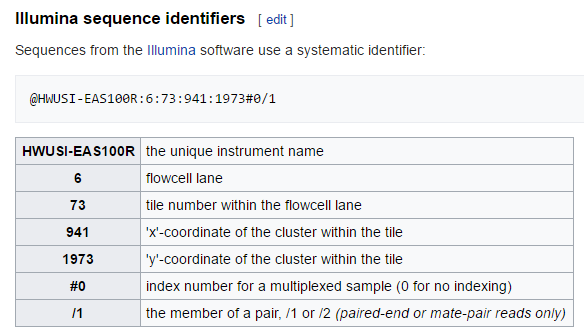
\includegraphics{figs/seq_id.png}
\caption{Seq id}
\end{figure}

Because we are mixing samples within a lane, we need a way to keep track
of the samples, such that we know which sequence belongs to Frank and
which belongs to Emily, despite many of their sequences sharing a lane.
The way we keep track is through barcoding, where we add a short
nucleotide sequence to the adapters used in PCR amplification. We
therefore create sequence libraries, with each library receiving its own
barcode, perform sequencing, and then parse these libraries using our
barcodes to reassign sequences to our original samples.

Look at the metadata mapping file below. This contains all of the
relevant sample information, as well as information associated with
sequencing, particularly barcode information.

\begin{Shaded}
\begin{Highlighting}[]
\NormalTok{MAP <-}\StringTok{ }\KeywordTok{read_delim}\NormalTok{(}\KeywordTok{file.path}\NormalTok{(data_dir,}\StringTok{'map.tsv'}\NormalTok{),}\StringTok{'}\CharTok{\textbackslash{}t}\StringTok{'}\NormalTok{)}
\end{Highlighting}
\end{Shaded}

\begin{verbatim}
## Parsed with column specification:
## cols(
##   `#SampleID` = col_character(),
##   BarcodeSequence = col_character(),
##   LinkerPrimerSequence = col_character(),
##   SampleType = col_character(),
##   Year = col_double(),
##   Month = col_double(),
##   Day = col_double(),
##   Subject = col_double(),
##   ReportedAntibioticUsage = col_character(),
##   DaysSinceExperimentStart = col_double(),
##   Description = col_character()
## )
\end{verbatim}

\begin{Shaded}
\begin{Highlighting}[]
\NormalTok{MAP[}\DecValTok{1}\NormalTok{:}\DecValTok{5}\NormalTok{,}\DecValTok{1}\NormalTok{:}\DecValTok{5}\NormalTok{]}
\end{Highlighting}
\end{Shaded}

\begin{verbatim}
## # A tibble: 5 x 5
##   `#SampleID` BarcodeSequence LinkerPrimerSequence SampleType  Year
##   <chr>       <chr>           <chr>                <chr>      <dbl>
## 1 L1S8        AGCTGACTAGTC    GTGCCAGCMGCCGCGGTAA  gut         2008
## 2 L1S140      ATGGCAGCTCTA    GTGCCAGCMGCCGCGGTAA  gut         2008
## 3 L1S57       ACACACTATGGC    GTGCCAGCMGCCGCGGTAA  gut         2009
## 4 L1S208      CTGAGATACGCG    GTGCCAGCMGCCGCGGTAA  gut         2009
## 5 L1S76       ACTACGTGTGGT    GTGCCAGCMGCCGCGGTAA  gut         2009
\end{verbatim}

We can see that each sample receives its own unique barcode:

\begin{Shaded}
\begin{Highlighting}[]
\KeywordTok{nrow}\NormalTok{(MAP[,}\DecValTok{1}\NormalTok{:}\DecValTok{2}\NormalTok{]) ==}\StringTok{ }\KeywordTok{nrow}\NormalTok{(}\KeywordTok{unique}\NormalTok{(MAP[,}\DecValTok{1}\NormalTok{:}\DecValTok{2}\NormalTok{]))}
\end{Highlighting}
\end{Shaded}

\begin{verbatim}
## [1] TRUE
\end{verbatim}

Now take a look at the barcode file:

\begin{Shaded}
\begin{Highlighting}[]
\NormalTok{BARCODE <-}\StringTok{ }\KeywordTok{readDNAStringSet}\NormalTok{(}\KeywordTok{file.path}\NormalTok{(data_dir,}\StringTok{'barcodes.fastq.gz'}\NormalTok{),}\DataTypeTok{format=}\StringTok{'fastq'}\NormalTok{)}
\NormalTok{BARCODE}
\end{Highlighting}
\end{Shaded}

\begin{verbatim}
##   A DNAStringSet instance of length 302581
##          width seq                                          names               
##      [1]    12 ATGCAGCTCAGT                                 HWI-EAS440_0386:1...
##      [2]    12 CCCCTCAGCGGC                                 HWI-EAS440_0386:1...
##      [3]    12 GACGAGTCAGTC                                 HWI-EAS440_0386:1...
##      [4]    12 AGCAGTCGCGAT                                 HWI-EAS440_0386:1...
##      [5]    12 AGCACACCTACA                                 HWI-EAS440_0386:1...
##      ...   ... ...
## [302577]    12 ATGGCTGTTGGT                                 HWI-EAS440_0386:6...
## [302578]    12 ACACACTATGGC                                 HWI-EAS440_0386:6...
## [302579]    12 CAGCGGTGACAT                                 HWI-EAS440_0386:6...
## [302580]    12 GATCTTCAGTAC                                 HWI-EAS440_0386:6...
## [302581]    12 GACAGCGTTGAC                                 HWI-EAS440_0386:6...
\end{verbatim}

We can see that each barcode is assigned one of the header names we saw
before. What we need to do now is break up this large fastq file that
contains all of our sequence information into a new large file that has
headers with unique \emph{sample IDs} for each sequence, for example,
Emily\_1, Emily\_2, and Emily\_3 for 3 sequences belonging to Emily. We
can easily do this in QIIME, but we first need to ensure that our
mapping file is formatted correctly; otherwise, QIIME will not run. We
can do that with the following command:

\begin{Shaded}
\begin{Highlighting}[]
\KeywordTok{system2}\NormalTok{(validate_mapping_file,}\DataTypeTok{args=}\KeywordTok{c}\NormalTok{(}\StringTok{'-m'}\NormalTok{,}\KeywordTok{file.path}\NormalTok{(data_dir,}\StringTok{'map.tsv'}\NormalTok{)))}
\end{Highlighting}
\end{Shaded}

Now, let's make some bad mapping files to see what happens. First, let's
simply remove the hashtag in the first column name:

\begin{Shaded}
\begin{Highlighting}[]
\NormalTok{MAP_bad1 <-}\StringTok{ }\NormalTok{MAP}
\KeywordTok{colnames}\NormalTok{(MAP_bad1)[}\DecValTok{1}\NormalTok{] <-}\StringTok{ 'SampleID'}

\NormalTok{tmp <-}\StringTok{ }\KeywordTok{tempfile}\NormalTok{()}
\KeywordTok{write_delim}\NormalTok{(MAP_bad1,}\DataTypeTok{path=}\NormalTok{tmp,}\DataTypeTok{delim=}\StringTok{'}\CharTok{\textbackslash{}t}\StringTok{'}\NormalTok{)}
\KeywordTok{system2}\NormalTok{(validate_mapping_file,}\DataTypeTok{args=}\KeywordTok{c}\NormalTok{(}\StringTok{'-m'}\NormalTok{,tmp))}
\end{Highlighting}
\end{Shaded}

Now, look what happens if we don't have a description column as the last
column:

\begin{Shaded}
\begin{Highlighting}[]
\NormalTok{MAP_bad2 <-}\StringTok{ }\NormalTok{MAP}
\NormalTok{MAP_bad2 <-}\StringTok{ }\NormalTok{MAP_bad2[,-}\KeywordTok{ncol}\NormalTok{(MAP_bad2)]}

\NormalTok{tmp <-}\StringTok{ }\KeywordTok{tempfile}\NormalTok{()}
\KeywordTok{write_delim}\NormalTok{(MAP_bad2,}\DataTypeTok{path=}\NormalTok{tmp,}\DataTypeTok{delim=}\StringTok{'}\CharTok{\textbackslash{}t}\StringTok{'}\NormalTok{)}
\KeywordTok{system2}\NormalTok{(validate_mapping_file,}\DataTypeTok{args=}\KeywordTok{c}\NormalTok{(}\StringTok{'-m'}\NormalTok{,tmp))}
\end{Highlighting}
\end{Shaded}

And lastly, what if we used separate with commas instead of tabs:

\begin{Shaded}
\begin{Highlighting}[]
\NormalTok{MAP_bad3 <-}\StringTok{ }\NormalTok{MAP}

\NormalTok{tmp <-}\StringTok{ }\KeywordTok{tempfile}\NormalTok{()}
\KeywordTok{write_delim}\NormalTok{(MAP_bad3,}\DataTypeTok{path=}\NormalTok{tmp,}\DataTypeTok{delim=}\StringTok{','}\NormalTok{)}
\KeywordTok{system2}\NormalTok{(validate_mapping_file,}\DataTypeTok{args=}\KeywordTok{c}\NormalTok{(}\StringTok{'-m'}\NormalTok{,tmp))}
\end{Highlighting}
\end{Shaded}

Given that we have a good mapping file, let's actually demultiplex our
data. The following QIIME command performs demultiplexing and also the
subsequent quality filtering. It also tosses out sequences that have
poor matches to a given barcode. All of these parameters we can adjust.

\begin{Shaded}
\begin{Highlighting}[]
\NormalTok{out <-}\StringTok{ }\KeywordTok{tempfile}\NormalTok{()}
\KeywordTok{system2}\NormalTok{(validate_mapping_file,}\DataTypeTok{args=}\KeywordTok{c}\NormalTok{(}\StringTok{'-m'}\NormalTok{,tmp,}
                                     \StringTok{'-o'}\NormalTok{,}\KeywordTok{file.path}\NormalTok{(data_dir,}\StringTok{'map_out'}\NormalTok{)))}

\KeywordTok{system2}\NormalTok{(split_libraries_fastq,}\DataTypeTok{args=}\KeywordTok{c}\NormalTok{(}\StringTok{'-o'}\NormalTok{,}\KeywordTok{file.path}\NormalTok{(data_dir,}\StringTok{'fastq_out_1'}\NormalTok{),}
                                     \StringTok{'-i'}\NormalTok{,}\KeywordTok{file.path}\NormalTok{(data_dir,}\StringTok{'forward_reads.fastq.gz'}\NormalTok{),}
                                     \StringTok{'-b'}\NormalTok{,}\KeywordTok{file.path}\NormalTok{(data_dir,}\StringTok{'barcodes.fastq.gz'}\NormalTok{),}
                                     \StringTok{'-m'}\NormalTok{,}\KeywordTok{file.path}\NormalTok{(data_dir,}\StringTok{'map.tsv'}\NormalTok{)))}
\end{Highlighting}
\end{Shaded}

Now, there are a few noteable filtering arguments:

\begin{itemize}
\tightlist
\item
  phred\_quality\_threshold
\item
  max\_bad\_run\_length
\item
  min\_per\_read\_length\_fraction
\end{itemize}

Phred score is defined as follows:

\[ 
Q=-10\log_{10}P 
\] where P is the probability of a base-call error; hence,

\[
P=10^{-Q/10}
\]

The default \textbf{phred\_quality\_threshold} Q is 3, implying
\(P=10^{-3/10}=.5\), or the probability of an incorrectly called base is
about 50\%. Setting it at 3 will flag any base call if it has a
probability of being an error above this threshold. For the entire
sequence, it will then look at \textbf{max\_bad\_run\_length}, which
checks how many \emph{consecutive} flagged base calls are present. If
this number is above a given threshold (the default is 3), then the
sequence is truncated at that position. Finally, it checks
\textbf{min\_per\_read\_length\_fraction}. This tosses any sequences
that are shorter than a given length after truncation (the default is a
length shorter than 75\% of the original, unaltered read).

There is also a setting called \textbf{phred offset}, which you
typically need not worry about (it's automatically set), but is worth
knowing what it represents:

\begin{figure}[htbp]
\centering
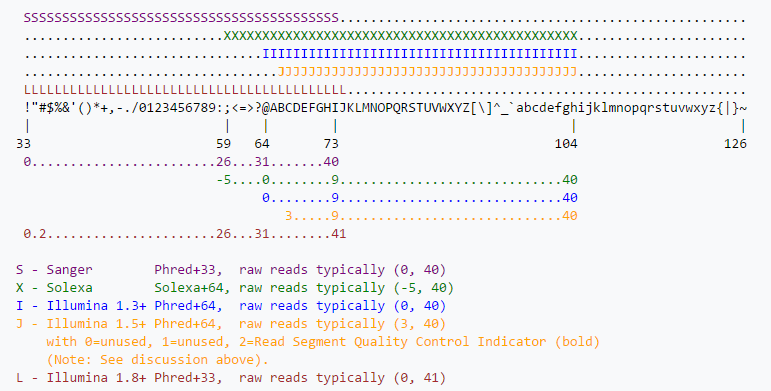
\includegraphics{figs/phred_offset.png}
\caption{Phred offset}
\end{figure}

I'd argue that something along the lines of Q=20 or greater makes more
sense. Here, we'll truncate at consecutive stretches of base calls where
each call has 1\% probability of being an error.

\begin{Shaded}
\begin{Highlighting}[]
\KeywordTok{system2}\NormalTok{(split_libraries_fastq,}\DataTypeTok{args=}\KeywordTok{c}\NormalTok{(}\StringTok{'-o'}\NormalTok{,}\KeywordTok{file.path}\NormalTok{(data_dir,}\StringTok{'fastq_out_2'}\NormalTok{),}
                                     \StringTok{'-i'}\NormalTok{,}\KeywordTok{file.path}\NormalTok{(data_dir,}\StringTok{'forward_reads.fastq.gz'}\NormalTok{),}
                                     \StringTok{'-b'}\NormalTok{,}\KeywordTok{file.path}\NormalTok{(data_dir,}\StringTok{'barcodes.fastq.gz'}\NormalTok{),}
                                     \StringTok{'-m'}\NormalTok{,}\KeywordTok{file.path}\NormalTok{(data_dir,}\StringTok{'map.tsv'}\NormalTok{),}
                                     \StringTok{'-q'}\NormalTok{,}\StringTok{'20'}\NormalTok{))}
\end{Highlighting}
\end{Shaded}

We'll now perform OTU picking on our filtered, demultiplexed sequences.
There are a ton of parameters we can adjust:
\url{http://qiime.org/scripts/pick_otus.html}. To keep it somewhat
simple, we'll perform a particular kind of OTU picking called `closed.'
There are 3 OTU picking strategies: closed, open, and de novo.

Closed reference OTU picking is fast because it simply clusters
sequences into OTUs based on reference sequences found in a database. If
a sequence doesn't match above a given similiary threshold to the
database sequence, it is tossed away. It should probably be obvious if a
given sequence isn't found in the reference database, it too will be
removed. De novo, on the other hand, can deal with novel sequences since
it doesn't use a lookup database. Instead, it clusters sequences by
aligning them against one another, with sequences above a given
similarity threshold clustered into OTUs. Lastly, open reference OTU
picking first performed closed reference OTU picking, and then performs
de novo on sequences that failed to match reference sequences in the
lookup database.

To perform closed reference OTU picking, we need to specify our
reference database (we'll use GreenGenes) by setting the location of our
reference sequences, our reference taxonomy. We also need to specify our
picking parameters, which in this example, will consist of the OTU
picking method (sortmerna), the number of threads for paralellization,
and the similarity threshold (.97) for our sequences when we compare
them to the GreenGenes database.

\begin{Shaded}
\begin{Highlighting}[]
\NormalTok{ref_seqs <-}\StringTok{ '/data/sw1/anaconda2/lib/python2.7/site-packages/qiime_default_reference/gg_13_8_otus/rep_set/97_otus.fasta'}
\NormalTok{ref_tax <-}\StringTok{ '/data/sw1/anaconda2/lib/python2.7/site-packages/qiime_default_reference/gg_13_8_otus/taxonomy/97_otu_taxonomy.txt'}

\NormalTok{params <-}\StringTok{ }\KeywordTok{tempfile}\NormalTok{(}\DataTypeTok{fileext=}\StringTok{'.txt'}\NormalTok{)}
\KeywordTok{write_lines}\NormalTok{(}\KeywordTok{c}\NormalTok{(}\StringTok{'pick_otus:otu_picking_method sortmerna'}\NormalTok{,}
              \StringTok{'pick_otus:threads 4'}\NormalTok{,}
              \StringTok{'pick_otus:similarity: 0.97'}\NormalTok{),}\DataTypeTok{path=}\NormalTok{params)}
\end{Highlighting}
\end{Shaded}

And now we run the closed reference otu picking command:

\begin{Shaded}
\begin{Highlighting}[]
\KeywordTok{system2}\NormalTok{(pick_closed_reference_otus,}\DataTypeTok{args=}\KeywordTok{c}\NormalTok{(}\StringTok{'-i'}\NormalTok{,}\KeywordTok{file.path}\NormalTok{(data_dir,}\StringTok{'fastq_out_2'}\NormalTok{,}\StringTok{'seqs.fna'}\NormalTok{),}
                                          \StringTok{'-o'}\NormalTok{,}\KeywordTok{file.path}\NormalTok{(data_dir,}\StringTok{'fastq_out_2'}\NormalTok{,}\StringTok{'picked_otus_sortmerna'}\NormalTok{),}
                                          \StringTok{'-r'}\NormalTok{,ref_seqs,}
                                          \StringTok{'-t'}\NormalTok{,ref_tax,}
                                          \StringTok{'-p'}\NormalTok{,params))}
\end{Highlighting}
\end{Shaded}

This was all done in R, which is probably unnecessary for proteus. You
can submit an Rscript, but since there is no real looping and need for
immediate downstream analysis, it's better off just submitting a bash
script. We'll remove the system2 functions and the like, add the
submission parameters, and write the following script for proteus:

\begin{Shaded}
\begin{Highlighting}[]
\CommentTok{#!/bin/bash}
\CommentTok{#$ -S /bin/bash}
\CommentTok{#$ -cwd}
\CommentTok{#$ -j y}
\CommentTok{#$ -M user_name@email.edu}
\CommentTok{#$ -l h_rt=01:00:00}
\CommentTok{#$ -P namePrj}
\CommentTok{#$ -pe shm 16}
\CommentTok{#$ -l mem_free=12G}
\CommentTok{#$ -l h_vmem=16G}
\CommentTok{#$ -q all.q}

\NormalTok{. /etc/profile.d/modules.sh}
\NormalTok{module load shared}
\NormalTok{module load proteus}
\NormalTok{module load sge/univa}
\NormalTok{module load gcc/}\FloatTok{4.8.1}
\NormalTok{module load qiime/gcc/}\DecValTok{64}\NormalTok{/}\FloatTok{1.9.1}

\NormalTok{export ref_seqs=}\ErrorTok{/}\NormalTok{mnt/HA/opt/qiime/gcc/}\DecValTok{64}\NormalTok{/}\FloatTok{1.9.1}\NormalTok{/lib/python2}\FloatTok{.7}\NormalTok{/site-packages/qiime_default_reference/gg_13_8_otus/rep_set/97_otus.fasta}
\NormalTok{export ref_tax=}\ErrorTok{/}\NormalTok{mnt/HA/opt/qiime/gcc/}\DecValTok{64}\NormalTok{/}\FloatTok{1.9.1}\NormalTok{/lib/python2}\FloatTok{.7}\NormalTok{/site-packages/qiime_default_reference/gg_13_8_otus/taxonomy/97_otu_taxonomy.txt}

\NormalTok{data_dir=}\ErrorTok{/}\NormalTok{home/user_name/genStats/moving_pictures}
\NormalTok{work_dir=}\ErrorTok{/}\NormalTok{scratch/user_name/moving_pictures}

\NormalTok{mkdir -p $work_dir}

\NormalTok{cp $data_dir/}\ErrorTok{*}\StringTok{ }\ErrorTok{$}\NormalTok{work_dir}

\NormalTok{out_dir=}\ErrorTok{$}\NormalTok{work_dir/fastq_out}
\NormalTok{seqs=}\ErrorTok{$}\NormalTok{work_dir/forward_reads.fastq.gz}
\NormalTok{bc=}\ErrorTok{$}\NormalTok{work_dir/barcodes.fastq.gz}
\NormalTok{map=}\ErrorTok{$}\NormalTok{work_dir/map.tsv}

\NormalTok{split_libraries_fastq.py -o $out_dir -i $seqs -b $bc -m $map -q }\DecValTok{20}

\NormalTok{params=}\ErrorTok{$}\NormalTok{work_dir/sortmerna_pick_params.txt}

\NormalTok{printf }\StringTok{"pick_otus:otu_picking_method sortmerna}\CharTok{\textbackslash{}n}\StringTok{pick_otus:threads 16}\CharTok{\textbackslash{}n}\StringTok{pick_otus:similarity 0.97"} \NormalTok{>}\StringTok{ }\ErrorTok{$}\NormalTok{params}

\NormalTok{pick_closed_reference_otus.py -i $out_dir/seqs.fna -o $out_dir/picked_otus -r $ref_seqs -t $ref_tax -p $params}

\NormalTok{mv $out_dir $data_dir}
\NormalTok{rm -r $work_dir/}\ErrorTok{*}
\StringTok{  }
\NormalTok{exit }\DecValTok{0}
\end{Highlighting}
\end{Shaded}

\subsection{Summarizing Our Results}\label{summarizing-our-results}

Now that we have our OTU table, in biom format, we can summarize our
results using some QIIME commands. First, let's look at the mapping file
to see what sample features we'd like to focus on:

\begin{Shaded}
\begin{Highlighting}[]
\KeywordTok{View}\NormalTok{(MAP)}
\end{Highlighting}
\end{Shaded}

Now, we'll write a submission script to get analyses output.

\begin{Shaded}
\begin{Highlighting}[]
\CommentTok{#!/bin/bash}
\CommentTok{#$ -S /bin/bash}
\CommentTok{#$ -cwd}
\CommentTok{#$ -j y}
\CommentTok{#$ -M user_name@email.edu}
\CommentTok{#$ -l h_rt=01:00:00}
\CommentTok{#$ -P namePrj}
\CommentTok{#$ -l mem_free=12G}
\CommentTok{#$ -l h_vmem=16G}
\CommentTok{#$ -q all.q}

\NormalTok{. /etc/profile.d/modules.sh}
\NormalTok{module load shared}
\NormalTok{module load proteus}
\NormalTok{module load sge/univa}
\NormalTok{module load gcc/}\FloatTok{4.8.1}
\NormalTok{module load qiime/gcc/}\DecValTok{64}\NormalTok{/}\FloatTok{1.9.1}

\NormalTok{export ref_seqs=}\ErrorTok{/}\NormalTok{mnt/HA/opt/qiime/gcc/}\DecValTok{64}\NormalTok{/}\FloatTok{1.9.1}\NormalTok{/lib/python2}\FloatTok{.7}\NormalTok{/site-packages/qiime_default_reference/gg_13_8_otus/rep_set/97_otus.fasta}
\NormalTok{export ref_tax=}\ErrorTok{/}\NormalTok{mnt/HA/opt/qiime/gcc/}\DecValTok{64}\NormalTok{/}\FloatTok{1.9.1}\NormalTok{/lib/python2}\FloatTok{.7}\NormalTok{/site-packages/qiime_default_reference/gg_13_8_otus/taxonomy/97_otu_taxonomy.txt}

\NormalTok{data_dir=}\ErrorTok{/}\NormalTok{home/user_name/genStats/moving_pictures}
\NormalTok{work_dir=}\ErrorTok{/}\NormalTok{scratch/user_name/moving_pictures}

\NormalTok{mkdir -p $work_dir}

\NormalTok{cp $data_dir/fastq_out/picked_otus/97_otus.tree $work_dir}
\NormalTok{cp $data_dir/fastq_out/picked_otus/otu_table.biom $work_dir}
\NormalTok{cp $data_dir/map.tsv $work_dir}

\NormalTok{otus=}\ErrorTok{$}\NormalTok{work_dir/otu_table.biom}
\NormalTok{tree=}\ErrorTok{$}\NormalTok{work_dir/97_otus.tree}
\NormalTok{map=}\ErrorTok{$}\NormalTok{work_dir/map.tsv}

\NormalTok{analysis_dir=}\ErrorTok{$}\NormalTok{work_dir/analysis}

\NormalTok{mkdir -p $analysis_dir}

\NormalTok{biom summarize-table -i $otus >}\StringTok{ }\ErrorTok{$}\NormalTok{analysis_dir/sampling_depth.dat}

\NormalTok{core_diversity_analyses.py -o $analysis_dir/diversity -i $otus -m $map -t $tree -c SampleType -e }\DecValTok{1000} \NormalTok{--recover_from_failure}

\NormalTok{mv $analysis_dir $data_dir}
\NormalTok{rm -r $work_dir/}\ErrorTok{*}
\StringTok{  }
\NormalTok{exit }\DecValTok{0}
\end{Highlighting}
\end{Shaded}

Or we can calculate the metrics more directly:

\begin{Shaded}
\begin{Highlighting}[]
\CommentTok{#!/bin/bash}
\CommentTok{#$ -S /bin/bash}
\CommentTok{#$ -cwd}
\CommentTok{#$ -j y}
\CommentTok{#$ -M user_name@email.edu}
\CommentTok{#$ -l h_rt=01:00:00}
\CommentTok{#$ -P namePrj}
\CommentTok{#$ -l mem_free=12G}
\CommentTok{#$ -l h_vmem=16G}
\CommentTok{#$ -q all.q}

\NormalTok{. /etc/profile.d/modules.sh}
\NormalTok{module load shared}
\NormalTok{module load proteus}
\NormalTok{module load sge/univa}
\NormalTok{module load gcc/}\FloatTok{4.8.1}
\NormalTok{module load qiime/gcc/}\DecValTok{64}\NormalTok{/}\FloatTok{1.9.1}

\NormalTok{data_dir=}\ErrorTok{/}\NormalTok{home/user_name/genStats/moving_pictures}
\NormalTok{work_dir=}\ErrorTok{/}\NormalTok{scratch/user_name/moving_pictures/}

\NormalTok{mkdir -p $work_dir}

\NormalTok{cp $data_dir/fastq_out/picked_otus/97_otus.tree $work_dir}
\NormalTok{cp $data_dir/fastq_out/picked_otus/otu_table.biom $work_dir}
\NormalTok{cp $data_dir/map.tsv $work_dir}

\NormalTok{otus=}\ErrorTok{$}\NormalTok{work_dir/otu_table.biom}
\NormalTok{tree=}\ErrorTok{$}\NormalTok{work_dir/97_otus.tree}
\NormalTok{map=}\ErrorTok{$}\NormalTok{work_dir/map.tsv}


\NormalTok{met_dir=}\ErrorTok{$}\NormalTok{work_dir/metrics}


\NormalTok{alpha_diversity.py -i $otus -t $tree -o $met_dir/alpha.txt}

\NormalTok{beta_diversity.py -i $otus -o $met_dir/beta -t $tree -m unweighted_unifrac}
\NormalTok{beta_diversity.py -i $otus -o $met_dir/beta -t $tree -m weighted_unifrac}

\NormalTok{principal_coordinates.py -i $met_dir/beta -o $met_dir/pcoa}

\NormalTok{make_2d_plots.py -i $met_dir/pcoa/pcoa_unweighted_unifrac_otu_table.txt -m $map -b SampleType -o $met_dir/pcoa/figures}
\NormalTok{make_2d_plots.py -i $met_dir/pcoa/pcoa_weighted_unifrac_otu_table.txt -m $map -b SampleType -o $met_dir/pcoa/figures}

\NormalTok{transform_coordinate_matrices.py -i $met_dir/pcoa/pcoa_unweighted_unifrac_otu_table.txt,$met_dir/pcoa/pcoa_weighted_unifrac_otu_table.txt -r }\DecValTok{999} \NormalTok{-o $met_dir/procrustes/}

\NormalTok{make_emperor.py -c -i $met_dir/procrustes -o $met_dir/procrustes/figures -m $map --custom_axes DaysSinceExperimentStart}

\NormalTok{mv $met_dir $data_dir}

\NormalTok{exit }\DecValTok{0}
\end{Highlighting}
\end{Shaded}

\subsection{Loading QIIME Results into
Phyloseq}\label{loading-qiime-results-into-phyloseq}

We have a ton of output from QIIME, but we could have just as easily
loaded the biom table into R, specifically phyloseq. We can do this like
so:

\begin{Shaded}
\begin{Highlighting}[]
\KeywordTok{library}\NormalTok{(phyloseq)}
\end{Highlighting}
\end{Shaded}

\begin{verbatim}
## 
## Attaching package: 'phyloseq'
\end{verbatim}

\begin{verbatim}
## The following object is masked from 'package:IRanges':
## 
##     distance
\end{verbatim}

\begin{Shaded}
\begin{Highlighting}[]
\NormalTok{biom_path <-}\StringTok{ }\KeywordTok{file.path}\NormalTok{(data_dir,}\StringTok{'fastq_out_2'}\NormalTok{,}\StringTok{'picked_otus_sortmerna'}\NormalTok{,}\StringTok{'otu_table.biom'}\NormalTok{)}
\NormalTok{tree_path <-}\StringTok{ }\KeywordTok{file.path}\NormalTok{(data_dir,}\StringTok{'fastq_out_2'}\NormalTok{,}\StringTok{'picked_otus_sortmerna'}\NormalTok{,}\StringTok{'97_otus.tree'}\NormalTok{)}

\NormalTok{BIOM <-}\StringTok{ }\KeywordTok{import_biom}\NormalTok{(biom_path)}
\end{Highlighting}
\end{Shaded}

\begin{verbatim}
## Warning in strsplit(conditionMessage(e), "\n"): input string 1 is invalid in
## this locale
\end{verbatim}

\begin{Shaded}
\begin{Highlighting}[]
\NormalTok{META <-}\StringTok{ }\KeywordTok{as.data.frame}\NormalTok{(MAP)}
\KeywordTok{rownames}\NormalTok{(META) <-}\StringTok{ }\NormalTok{META$}\StringTok{`}\DataTypeTok{#SampleID}\StringTok{`}
\NormalTok{PS <-}\StringTok{ }\KeywordTok{merge_phyloseq}\NormalTok{(BIOM,}\KeywordTok{sample_data}\NormalTok{(META))}
\NormalTok{PS}
\end{Highlighting}
\end{Shaded}

\begin{verbatim}
## phyloseq-class experiment-level object
## otu_table()   OTU Table:         [ 3409 taxa and 34 samples ]
## sample_data() Sample Data:       [ 34 samples by 11 sample variables ]
## tax_table()   Taxonomy Table:    [ 3409 taxa by 7 taxonomic ranks ]
\end{verbatim}

And then perform similar analyses:

\begin{Shaded}
\begin{Highlighting}[]
\KeywordTok{plot_ordination}\NormalTok{(PS,}\KeywordTok{ordinate}\NormalTok{(PS,}\DataTypeTok{method=}\StringTok{'MDS'}\NormalTok{,}\DataTypeTok{distance=}\StringTok{'bray'}\NormalTok{),}\DataTypeTok{type=}\StringTok{'samples'}\NormalTok{,}\DataTypeTok{color=}\StringTok{'SampleType'}\NormalTok{)}
\end{Highlighting}
\end{Shaded}

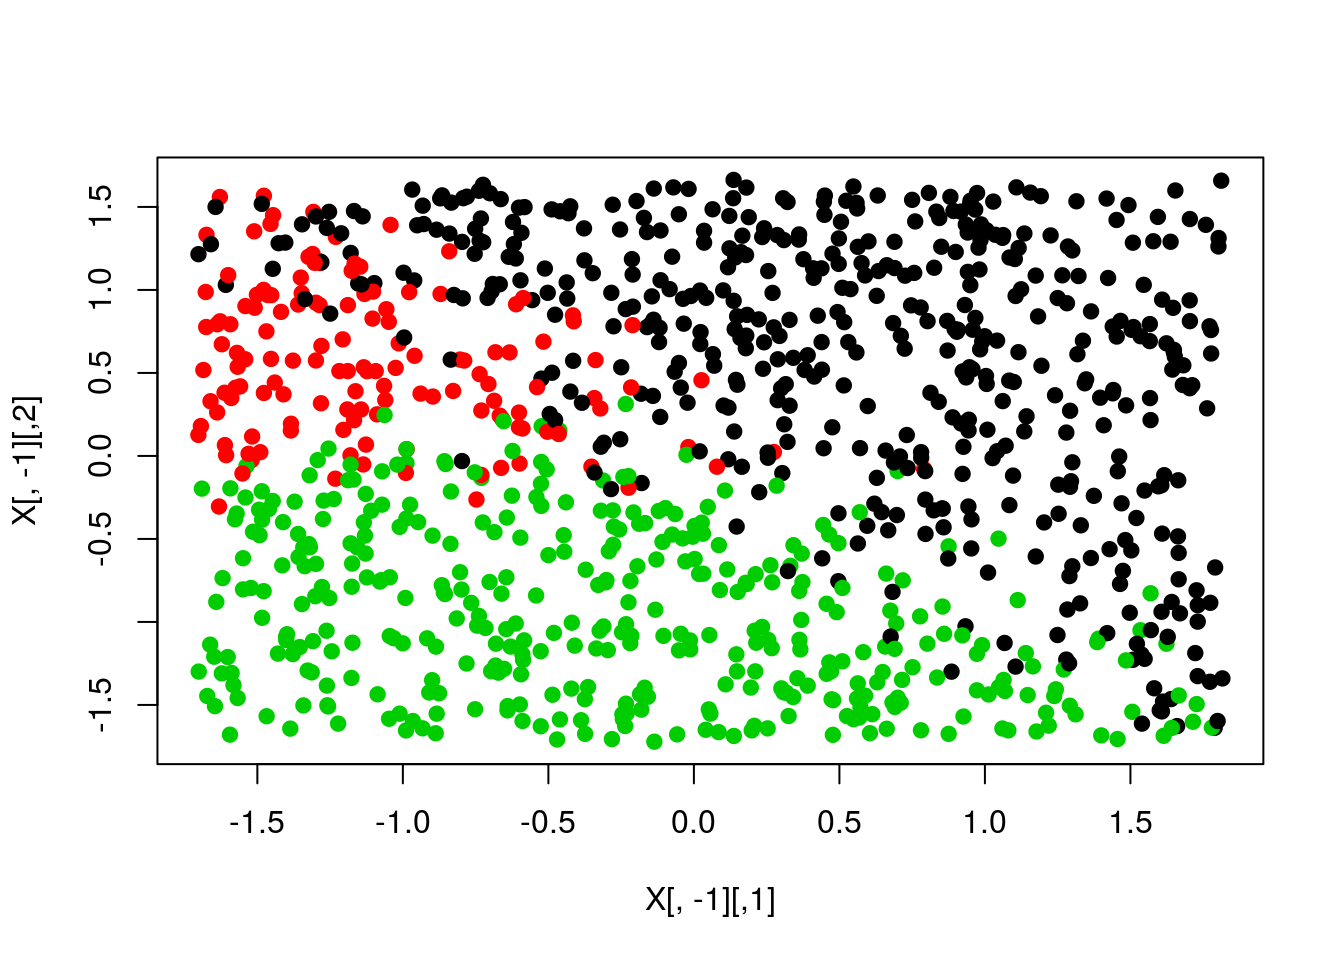
\includegraphics{08_qiime_files/figure-latex/unnamed-chunk-24-1.pdf}

\section{Multiple Comparisons}\label{multcomp}

\begin{Shaded}
\begin{Highlighting}[]
\KeywordTok{library}\NormalTok{(tidyverse)}
\KeywordTok{library}\NormalTok{(shiny)}
\end{Highlighting}
\end{Shaded}

\subsection{Hypothesis Testing and
Power}\label{hypothesis-testing-and-power}

When we perform a statistical hypothesis test, we measure a given
effect, assess its probability of occuring given a null hypothesis
\(H_0\) (i.e., the hypothesis that there is \emph{no} relationship
between our test groupings), and reject said null if the probability
falls below a particular threshold. We ``accept'' \(H_1\) and consider
this test to be \emph{statistically significant}. We aren't always
right, however; hence, hypothesis testing is prone to \emph{false
positives (type I errors) and false negatives (type II errors)}:

\begin{longtable}[c]{@{}lll@{}}
\toprule
& \textbf{Reject} \(H_0\) & \textbf{Reject} \(H_1\)\tabularnewline
\midrule
\endhead
\textbf{False} \(H_0\) & True Positives (TP) & False Negatives
(FN)\tabularnewline
\textbf{True} \(H_0\) & False Positives (FP) & True Negatives
(TN)\tabularnewline
\bottomrule
\end{longtable}

You'll often see the false positive error probability refered to as
\(\alpha\) (where \(\alpha=\frac{\text{FP}}{\text{FP}+\text{TN}}\)), the
false negative error probability referred to as \(\beta\) (where
\(\beta=\frac{\text{FN}}{\text{FN}+\text{TP}}\)), and the
\textbf{probabilty of a false negative not occuring} as \(1-\beta\).
Tests that have low \(beta\) are said to have high \emph{power}, where
\(\text{Power}=1-\beta\). One can interpret a powerful test as a test
that is very capable of detecting when the null hypothesis is false --
that is, \(P(\text{reject } H_0|\text{true } H_1)\). If we were
comparing two groups, and our power was about 0.9, then we'd have about
a 90\% chance of detecting a difference between the groups and a 10\%
chance of missing it.

\subsection{Multiple Comparisons}\label{multiple-comparisons}

Whether you continue to work with large datasets or transition into the
types of data problems one often sees stemming from benchwork, you'll
come across the multiple comparisons problem. Let's focus on a situation
common when working with DNA or RNA sequencing counts. Say we were given
some \(N \times M\) normalized gene table, where there are \(N=100\)
samples and \(M=10000\) genes. Of these samples, 50 will belong to group
1 and the other 50 to group 2:

\begin{Shaded}
\begin{Highlighting}[]
\NormalTok{N_grp1 <-}\StringTok{ }\DecValTok{50}
\NormalTok{N_grp2 <-}\StringTok{ }\DecValTok{50}
\NormalTok{N <-}\StringTok{ }\NormalTok{N_grp1+N_grp2}
\NormalTok{M <-}\StringTok{ }\DecValTok{10000}

\KeywordTok{set.seed}\NormalTok{(}\DecValTok{453}\NormalTok{)}
\NormalTok{TABLE_grp1 <-}\StringTok{ }\KeywordTok{matrix}\NormalTok{(}\KeywordTok{rnorm}\NormalTok{(N_grp1*M,}\DecValTok{0}\NormalTok{,}\DecValTok{1}\NormalTok{),N_grp1,M,}\DataTypeTok{dimnames=}\KeywordTok{list}\NormalTok{(}\KeywordTok{paste0}\NormalTok{(}\StringTok{'sample'}\NormalTok{,}\DecValTok{1}\NormalTok{:N_grp1),}\KeywordTok{paste0}\NormalTok{(}\StringTok{'gene'}\NormalTok{,}\DecValTok{1}\NormalTok{:M)))}
\NormalTok{TABLE_grp2 <-}\StringTok{ }\KeywordTok{matrix}\NormalTok{(}\KeywordTok{rnorm}\NormalTok{(N_grp2*M,}\DecValTok{0}\NormalTok{,}\DecValTok{1}\NormalTok{),N_grp2,M,}\DataTypeTok{dimnames=}\KeywordTok{list}\NormalTok{(}\KeywordTok{paste0}\NormalTok{(}\StringTok{'sample'}\NormalTok{,}\DecValTok{1}\NormalTok{:N_grp2),}\KeywordTok{paste0}\NormalTok{(}\StringTok{'gene'}\NormalTok{,}\DecValTok{1}\NormalTok{:M)))}
\NormalTok{TABLE <-}\StringTok{ }\KeywordTok{rbind}\NormalTok{(TABLE_grp1,TABLE_grp2)}
\end{Highlighting}
\end{Shaded}

Now, let's aim to identify important genes that are different between
the two groups. We can do this by performing a t test between the groups
for each gene sequentially. I'm going to hardcode the t test there in
case you are unfamiliar.

\begin{Shaded}
\begin{Highlighting}[]
\NormalTok{tstats <-}\StringTok{ }\KeywordTok{vector}\NormalTok{(}\DataTypeTok{mode=}\StringTok{'double'}\NormalTok{,}\DataTypeTok{length=}\NormalTok{M)}
\NormalTok{for (gene in }\KeywordTok{seq_len}\NormalTok{(M))\{}
  \NormalTok{grp1 <-}\StringTok{ }\NormalTok{TABLE[}\DecValTok{1}\NormalTok{:}\DecValTok{50}\NormalTok{,gene]}
  \NormalTok{grp2 <-}\StringTok{ }\NormalTok{TABLE[}\DecValTok{51}\NormalTok{:}\DecValTok{100}\NormalTok{,gene]}
  
  \NormalTok{mu1 <-}\StringTok{ }\KeywordTok{mean}\NormalTok{(grp1)}
  \NormalTok{mu2 <-}\StringTok{ }\KeywordTok{mean}\NormalTok{(grp2)}
  
  \NormalTok{v1 <-}\StringTok{ }\KeywordTok{sum}\NormalTok{((grp1 -}\StringTok{ }\KeywordTok{mean}\NormalTok{(grp1))^}\DecValTok{2}\NormalTok{)}
  \NormalTok{v2 <-}\StringTok{ }\KeywordTok{sum}\NormalTok{((grp2 -}\StringTok{ }\KeywordTok{mean}\NormalTok{(grp2))^}\DecValTok{2}\NormalTok{)}
  
  \NormalTok{s2 <-}\StringTok{ }\NormalTok{(}\DecValTok{1}\NormalTok{/(N}\DecValTok{-2}\NormalTok{))*(v1 +}\StringTok{ }\NormalTok{v2)}
  \NormalTok{se <-}\StringTok{ }\KeywordTok{sqrt}\NormalTok{(s2*(}\DecValTok{1}\NormalTok{/N_grp1 +}\StringTok{ }\DecValTok{1}\NormalTok{/N_grp2))}
  
  \NormalTok{tstats[gene] <-}\StringTok{ }\NormalTok{(mu1-mu2)/se}
\NormalTok{\}}
\end{Highlighting}
\end{Shaded}

And now we can plot it.

\begin{Shaded}
\begin{Highlighting}[]
\KeywordTok{qplot}\NormalTok{(tstats,}\DataTypeTok{geom=}\StringTok{'histogram'}\NormalTok{,}\DataTypeTok{color=}\KeywordTok{I}\NormalTok{(}\StringTok{'black'}\NormalTok{),}\DataTypeTok{bins=}\DecValTok{50}\NormalTok{)}
\end{Highlighting}
\end{Shaded}

\includegraphics{09_multiple_comparisons_files/figure-latex/unnamed-chunk-5-1.pdf}

Clearly the t statistics are normally distributed. The typical approach
with t tests is to perform a hypothesis test at the 5\% significance
level, such that we reject any null hypothesis with t statistics more
than 2 standard deviations from the mode in either direction of this
distribution. We use 2 standard deviations because qnorm(0.975) is 1.96
and qnorm(0.025) is -1.96:

\begin{Shaded}
\begin{Highlighting}[]
\KeywordTok{qplot}\NormalTok{(tstats,}\DataTypeTok{geom=}\StringTok{'histogram'}\NormalTok{,}\DataTypeTok{color=}\KeywordTok{I}\NormalTok{(}\StringTok{'black'}\NormalTok{),}\DataTypeTok{bins=}\DecValTok{50}\NormalTok{) +}
\StringTok{  }\KeywordTok{geom_vline}\NormalTok{(}\DataTypeTok{xintercept=}\KeywordTok{qnorm}\NormalTok{(}\FloatTok{0.025}\NormalTok{),}\DataTypeTok{linetype=}\DecValTok{2}\NormalTok{,}\DataTypeTok{color=}\StringTok{'red'}\NormalTok{) +}
\StringTok{  }\KeywordTok{geom_vline}\NormalTok{(}\DataTypeTok{xintercept=}\KeywordTok{qnorm}\NormalTok{(}\FloatTok{0.975}\NormalTok{),}\DataTypeTok{linetype=}\DecValTok{2}\NormalTok{,}\DataTypeTok{color=}\StringTok{'red'}\NormalTok{)}
\end{Highlighting}
\end{Shaded}

\includegraphics{09_multiple_comparisons_files/figure-latex/unnamed-chunk-6-1.pdf}

It should be apparent that there are quite a few significant genes. If
you were paying attention to how our groups were generated, this should
be surprising to you. We generated both groups from the \emph{same}
normal distribution. Nevertheless, we still have a ton of significant
genes:

\begin{Shaded}
\begin{Highlighting}[]
\KeywordTok{sum}\NormalTok{(tstats<}\KeywordTok{qnorm}\NormalTok{(}\FloatTok{0.025}\NormalTok{) |}\StringTok{ }\NormalTok{tstats>}\KeywordTok{qnorm}\NormalTok{(}\FloatTok{0.975}\NormalTok{))}
\end{Highlighting}
\end{Shaded}

\begin{verbatim}
## [1] 530
\end{verbatim}

So over 500 genes were significant despite the fact that we know there
is no underlying effect. Well, this is actually quite consistent with
the defiinition of a p value. Given a typical hypothesis test, we reject
the null if the probability of the observation is less than the
probability of the observation occuring assuming the null hypothesis is
true. In other words, we reject the claim that there is no statistical
effect if our p value is less than (in absolute value) \(\alpha\), the
probability of a statistical effect due to random sampling variation.
Therefore, because there are 10,000 genes and hence we perform 10,000 t
tests, givin an \(\alpha\) of 0.05, we should expect about
\(0.05 \times 10000 = 500\) significant t statistics due to random
sampling variation alone, which is the case here.

So that's all well and good. We now know that if we set \(\alpha\) at a
particular level, given our null and sample size, we should expect some
false positives. But is that enough information? Let's rerun the above
model, but now with an actual difference between groups:

\begin{Shaded}
\begin{Highlighting}[]
\NormalTok{N_grp1 <-}\StringTok{ }\DecValTok{50}
\NormalTok{N_grp2 <-}\StringTok{ }\DecValTok{50}
\NormalTok{N <-}\StringTok{ }\NormalTok{N_grp1+N_grp2}
\NormalTok{M <-}\StringTok{ }\DecValTok{10000}

\KeywordTok{set.seed}\NormalTok{(}\DecValTok{65}\NormalTok{)}
\NormalTok{TABLE_grp1 <-}\StringTok{ }\KeywordTok{matrix}\NormalTok{(}\KeywordTok{rnorm}\NormalTok{(N_grp1*M,.}\DecValTok{25}\NormalTok{,}\DecValTok{2}\NormalTok{),N_grp1,M,}\DataTypeTok{dimnames=}\KeywordTok{list}\NormalTok{(}\KeywordTok{paste0}\NormalTok{(}\StringTok{'sample'}\NormalTok{,}\DecValTok{1}\NormalTok{:N_grp1),}\KeywordTok{paste0}\NormalTok{(}\StringTok{'gene'}\NormalTok{,}\DecValTok{1}\NormalTok{:M)))}
\NormalTok{TABLE_grp2 <-}\StringTok{ }\KeywordTok{matrix}\NormalTok{(}\KeywordTok{rnorm}\NormalTok{(N_grp2*M,-.}\DecValTok{25}\NormalTok{,}\DecValTok{2}\NormalTok{),N_grp2,M,}\DataTypeTok{dimnames=}\KeywordTok{list}\NormalTok{(}\KeywordTok{paste0}\NormalTok{(}\StringTok{'sample'}\NormalTok{,}\DecValTok{1}\NormalTok{:N_grp2),}\KeywordTok{paste0}\NormalTok{(}\StringTok{'gene'}\NormalTok{,}\DecValTok{1}\NormalTok{:M)))}
\NormalTok{TABLE <-}\StringTok{ }\KeywordTok{rbind}\NormalTok{(TABLE_grp1,TABLE_grp2)}

\NormalTok{tstats <-}\StringTok{ }\KeywordTok{vector}\NormalTok{(}\DataTypeTok{mode=}\StringTok{'double'}\NormalTok{,}\DataTypeTok{length=}\NormalTok{M)}
\NormalTok{tstats2 <-}\StringTok{ }\KeywordTok{vector}\NormalTok{(}\DataTypeTok{mode=}\StringTok{'double'}\NormalTok{,}\DataTypeTok{length=}\NormalTok{M)}
\NormalTok{for (gene in }\KeywordTok{seq_len}\NormalTok{(M))\{}
  \NormalTok{grp1 <-}\StringTok{ }\NormalTok{TABLE[}\DecValTok{1}\NormalTok{:}\DecValTok{50}\NormalTok{,gene]}
  \NormalTok{grp2 <-}\StringTok{ }\NormalTok{TABLE[}\DecValTok{51}\NormalTok{:}\DecValTok{100}\NormalTok{,gene]}
  
  \NormalTok{mu1 <-}\StringTok{ }\KeywordTok{mean}\NormalTok{(grp1)}
  \NormalTok{mu2 <-}\StringTok{ }\KeywordTok{mean}\NormalTok{(grp2)}
  
  \NormalTok{v1 <-}\StringTok{ }\KeywordTok{sum}\NormalTok{((grp1 -}\StringTok{ }\KeywordTok{mean}\NormalTok{(grp1))^}\DecValTok{2}\NormalTok{)}
  \NormalTok{v2 <-}\StringTok{ }\KeywordTok{sum}\NormalTok{((grp2 -}\StringTok{ }\KeywordTok{mean}\NormalTok{(grp2))^}\DecValTok{2}\NormalTok{)}
  
  \NormalTok{s2 <-}\StringTok{ }\NormalTok{(}\DecValTok{1}\NormalTok{/(N}\DecValTok{-2}\NormalTok{))*(v1 +}\StringTok{ }\NormalTok{v2)}
  \NormalTok{se <-}\StringTok{ }\KeywordTok{sqrt}\NormalTok{(s2*(}\DecValTok{1}\NormalTok{/N_grp1 +}\StringTok{ }\DecValTok{1}\NormalTok{/N_grp2))}
  
  \NormalTok{tstats[gene] <-}\StringTok{ }\NormalTok{(mu1-mu2)/se}
\NormalTok{\}}

\KeywordTok{sum}\NormalTok{(tstats<}\KeywordTok{qnorm}\NormalTok{(}\FloatTok{0.025}\NormalTok{) |}\StringTok{ }\NormalTok{tstats>}\KeywordTok{qnorm}\NormalTok{(}\FloatTok{0.975}\NormalTok{))}
\end{Highlighting}
\end{Shaded}

\begin{verbatim}
## [1] 2386
\end{verbatim}

Now the two groups have different normlized gene values, which leads to
over 2000 significant genes. We know from before that about 500 should
be due to random sampling variation, but how do we know which ones? This
brings us to methods to adjust our results such that we can interpret
them more easily.

\subsubsection{Bonferroni}\label{bonferroni}

We'll start with Bonferroni correction. First thing we'll do is
calculate the p values for all of those t statistics:

\begin{Shaded}
\begin{Highlighting}[]
\NormalTok{pvals <-}\StringTok{ }\DecValTok{2}\NormalTok{*(}\DecValTok{1}\NormalTok{-}\KeywordTok{pt}\NormalTok{(tstats,N}\DecValTok{-2}\NormalTok{))}
\end{Highlighting}
\end{Shaded}

Let's continue to assume \(\alpha=0.05\). Now, we should have
\emph{about} the same number of significant genes as mentioned before:

\begin{Shaded}
\begin{Highlighting}[]
\NormalTok{alpha <-}\StringTok{ }\NormalTok{.}\DecValTok{05}
\KeywordTok{sum}\NormalTok{(pvals <}\StringTok{ }\NormalTok{alpha)}
\end{Highlighting}
\end{Shaded}

\begin{verbatim}
## [1] 2309
\end{verbatim}

Bonferroni corrects for multiple comparisons by controlling for the
\emph{family-wise error rate (FWER)} -- the probability of making at
least one false positive -- by simply dividing \(\alpha\) by the number
of tests performed, which gives a new, adjusted \(\alpha\) to use as a
significance threshold:

\begin{Shaded}
\begin{Highlighting}[]
\NormalTok{alpha_bonf <-}\StringTok{ }\NormalTok{alpha/M}
\KeywordTok{sum}\NormalTok{(pvals <}\StringTok{ }\NormalTok{alpha_bonf)}
\end{Highlighting}
\end{Shaded}

\begin{verbatim}
## [1] 5
\end{verbatim}

This gives us only 2 significant genes. We should expect more given the
way we set the group means. The issue with using Bonferonni here is that
it's quite \textbf{conservative}, and tends to really \textbf{decrease
statistical power} when there are a lot of tests, as in this case.
Consequently, we are likely to see a ton of \textbf{false negatives}. In
the cases where we perform only a few tests (say 10 or less), Bonferonni
is quick and easy, and probably appropriate, but definitely not here.

\subsubsection{False Discovery Rate}\label{false-discovery-rate}

Instead of controlling for the family-wise error rate, we can control
for the \emph{false discovery rate (FDR)}, the expected proportion of
false positives. Unlike the FWER, which provides stringent control over
false positives, the FDR is far more lenient, thereby \emph{increasing
power at the sacrifice for more false positives}.

If we rewrite our table from above as follows:

\begin{longtable}[c]{@{}llll@{}}
\toprule
& \textbf{Reject} \(H_0\) & \textbf{Reject} \(H_1\) &
\textbf{Total}\tabularnewline
\midrule
\endhead
\textbf{False} \(H_0\) & True Positives (TP) & False Negatives (FN) &
Actual Positives (AP)\tabularnewline
\textbf{True} \(H_0\) & False Positives (FP) & True Negatives (TN) &
Actual Negatives (AN)\tabularnewline
\textbf{Total} & Called Positives (CP) & Called Negatives (CN) & Total
(TOTAL)\tabularnewline
\bottomrule
\end{longtable}

we can rewrite the FDR as \[
\text{FDR}=\mathop{\mathbb{E}}\left[\frac{\text{FP}}{\text{CP}}\right]
\].

Assuming all of our tests are independent, and given a significance
threshold \(\alpha\), the FDR has the following property

\[
\text{FDR}=\mathop{\mathbb{E}}\left[\frac{\text{FP}}{\text{CP}}\right] \le \alpha\frac{\text{AN}}{\text{TOTAL}} \le \alpha
\] Below is a figure to show what FDR correction will ultimately do to
our dataset we generated above.

\begin{Shaded}
\begin{Highlighting}[]
\NormalTok{alpha <-}\StringTok{ }\NormalTok{.}\DecValTok{05}
\NormalTok{df <-}\StringTok{ }\KeywordTok{data.frame}\NormalTok{(}\DataTypeTok{gene=}\DecValTok{1}\NormalTok{:}\KeywordTok{length}\NormalTok{(pvals),}
                 \DataTypeTok{p=}\KeywordTok{sort}\NormalTok{(pvals),}
                 \DataTypeTok{fit=}\NormalTok{(}\DecValTok{1}\NormalTok{:}\KeywordTok{length}\NormalTok{(pvals))*alpha/M)}
\KeywordTok{ggplot}\NormalTok{(df,}\KeywordTok{aes}\NormalTok{(gene,p)) +}
\StringTok{  }\KeywordTok{geom_vline}\NormalTok{(}\DataTypeTok{xintercept=}\KeywordTok{sum}\NormalTok{(pvals <}\StringTok{ }\NormalTok{alpha),}\DataTypeTok{size=}\NormalTok{.}\DecValTok{5}\NormalTok{) +}
\StringTok{  }\KeywordTok{geom_vline}\NormalTok{(}\DataTypeTok{xintercept=}\NormalTok{alpha*M,}\DataTypeTok{size=}\NormalTok{.}\DecValTok{5}\NormalTok{) +}
\StringTok{  }\KeywordTok{geom_line}\NormalTok{(}\KeywordTok{aes}\NormalTok{(gene,fit),}\DataTypeTok{color=}\StringTok{'red'}\NormalTok{,}\DataTypeTok{linetype=}\DecValTok{3}\NormalTok{,}\DataTypeTok{size=}\NormalTok{.}\DecValTok{5}\NormalTok{) +}
\StringTok{  }\KeywordTok{geom_point}\NormalTok{(}\DataTypeTok{size=}\NormalTok{.}\DecValTok{3}\NormalTok{) +}\StringTok{ }
\StringTok{  }\KeywordTok{scale_x_log10}\NormalTok{() +}\StringTok{ }\KeywordTok{scale_y_log10}\NormalTok{() +}\StringTok{ }\KeywordTok{labs}\NormalTok{(}\DataTypeTok{x=}\StringTok{'Genes'}\NormalTok{,}\DataTypeTok{y=}\StringTok{'Log10 p Value'}\NormalTok{) +}
\StringTok{  }\KeywordTok{annotate}\NormalTok{(}\StringTok{'label'}\NormalTok{,}\KeywordTok{sum}\NormalTok{(pvals <}\StringTok{ }\NormalTok{alpha),}\FloatTok{1e-06}\NormalTok{,}\DataTypeTok{label=}\StringTok{'alpha'}\NormalTok{,}\DataTypeTok{parse=}\OtherTok{TRUE}\NormalTok{) +}
\StringTok{  }\KeywordTok{annotate}\NormalTok{(}\StringTok{'label'}\NormalTok{,alpha*M,}\FloatTok{1e-06}\NormalTok{,}\DataTypeTok{label=}\StringTok{'alpha*M'}\NormalTok{,}\DataTypeTok{parse=}\OtherTok{TRUE}\NormalTok{)}
\end{Highlighting}
\end{Shaded}

\includegraphics{09_multiple_comparisons_files/figure-latex/unnamed-chunk-12-1.pdf}

The genes are ordered in terms of increasing p value, with everything on
log scale. The vertical lines shows the number of genes with
\(p<\alpha\) and the number of genes we should expect based on random
sampling alone, \(\alpha*M\), where M is our total number of genes. The
red diagonal line is the gene index multiplied by
\(\alpha/\text{TOTAL}\). This gives us the FDR threshold. Any genes that
fall \emph{below} this line are considered significant after FDR
adjustment.

To perform this adjustment, we simply choose an alpha, then rank our M
genes in terms of increasing p value and identify the largest p value
for genes where

\[
p_\text{gene} < \alpha \frac{\text{rank}}{M}
\] This becomes our new significance threshold:

\begin{Shaded}
\begin{Highlighting}[]
\NormalTok{alpha_fdr <-}\StringTok{ }\KeywordTok{max}\NormalTok{(df$p[df$p <}\StringTok{ }\NormalTok{alpha*df$gene/M])}
\KeywordTok{sum}\NormalTok{(pvals<alpha_fdr)}
\end{Highlighting}
\end{Shaded}

\begin{verbatim}
## [1] 222
\end{verbatim}

This results in far more significant genes than the Bonferroni methods,
but still less than half of what we'd expect from random sampling
variation.

\begin{Shaded}
\begin{Highlighting}[]
\KeywordTok{ggplot}\NormalTok{(df,}\KeywordTok{aes}\NormalTok{(gene,p)) +}
\StringTok{  }\KeywordTok{geom_vline}\NormalTok{(}\DataTypeTok{xintercept=}\KeywordTok{sum}\NormalTok{(pvals <}\StringTok{ }\NormalTok{alpha),}\DataTypeTok{size=}\NormalTok{.}\DecValTok{5}\NormalTok{) +}
\StringTok{  }\KeywordTok{geom_vline}\NormalTok{(}\DataTypeTok{xintercept=}\NormalTok{alpha*M,}\DataTypeTok{size=}\NormalTok{.}\DecValTok{5}\NormalTok{) +}
\StringTok{  }\KeywordTok{geom_vline}\NormalTok{(}\DataTypeTok{xintercept=}\KeywordTok{sum}\NormalTok{(pvals <}\StringTok{ }\NormalTok{alpha_bonf),}\DataTypeTok{size=}\NormalTok{.}\DecValTok{5}\NormalTok{,}\DataTypeTok{color=}\StringTok{'blue'}\NormalTok{) +}
\StringTok{  }\KeywordTok{geom_vline}\NormalTok{(}\DataTypeTok{xintercept=}\KeywordTok{sum}\NormalTok{(pvals <}\StringTok{ }\NormalTok{alpha_fdr),}\DataTypeTok{size=}\NormalTok{.}\DecValTok{5}\NormalTok{,}\DataTypeTok{color=}\StringTok{'darkgreen'}\NormalTok{) +}
\StringTok{  }\KeywordTok{geom_line}\NormalTok{(}\KeywordTok{aes}\NormalTok{(gene,fit),}\DataTypeTok{color=}\StringTok{'red'}\NormalTok{,}\DataTypeTok{linetype=}\DecValTok{3}\NormalTok{,}\DataTypeTok{size=}\NormalTok{.}\DecValTok{5}\NormalTok{) +}
\StringTok{  }\KeywordTok{geom_point}\NormalTok{(}\DataTypeTok{size=}\NormalTok{.}\DecValTok{3}\NormalTok{) +}\StringTok{ }
\StringTok{  }\KeywordTok{scale_x_log10}\NormalTok{() +}\StringTok{ }\KeywordTok{scale_y_log10}\NormalTok{() +}\StringTok{ }\KeywordTok{labs}\NormalTok{(}\DataTypeTok{x=}\StringTok{'Genes'}\NormalTok{,}\DataTypeTok{y=}\StringTok{'Log10 p Value'}\NormalTok{) +}
\StringTok{  }\KeywordTok{annotate}\NormalTok{(}\StringTok{'label'}\NormalTok{,}\KeywordTok{sum}\NormalTok{(pvals <}\StringTok{ }\NormalTok{alpha),}\FloatTok{1e-06}\NormalTok{,}\DataTypeTok{label=}\StringTok{'alpha'}\NormalTok{,}\DataTypeTok{parse=}\OtherTok{TRUE}\NormalTok{) +}
\StringTok{  }\KeywordTok{annotate}\NormalTok{(}\StringTok{'label'}\NormalTok{,alpha*M,}\FloatTok{1e-06}\NormalTok{,}\DataTypeTok{label=}\StringTok{'alpha*M'}\NormalTok{,}\DataTypeTok{parse=}\OtherTok{TRUE}\NormalTok{) +}
\StringTok{  }\KeywordTok{annotate}\NormalTok{(}\StringTok{'label'}\NormalTok{,}\KeywordTok{sum}\NormalTok{(pvals <}\StringTok{ }\NormalTok{alpha_bonf),}\FloatTok{1e-06}\NormalTok{,}\DataTypeTok{label=}\StringTok{'alpha[bonf]'}\NormalTok{,}\DataTypeTok{parse=}\OtherTok{TRUE}\NormalTok{) +}
\StringTok{  }\KeywordTok{annotate}\NormalTok{(}\StringTok{'label'}\NormalTok{,}\KeywordTok{sum}\NormalTok{(pvals <}\StringTok{ }\NormalTok{alpha_fdr),}\FloatTok{1e-06}\NormalTok{,}\DataTypeTok{label=}\StringTok{'alpha[fdr]'}\NormalTok{,}\DataTypeTok{parse=}\OtherTok{TRUE}\NormalTok{)}
\end{Highlighting}
\end{Shaded}

\includegraphics{09_multiple_comparisons_files/figure-latex/unnamed-chunk-14-1.pdf}

\section{Lasso}\label{lasso}

\subsection{Big Data and Feature
Selection}\label{big-data-and-feature-selection}

A common hurdle found when dealing with big data is determining which
covariates are relevant prior to model fitting. One could fit a full
model, but when dimensionality of the potential features reaches the
order of thousands, both the demand on computational resources and time
often makes such a strategy impractical. Choosing relevant features
ahead of time allows the user to simultaneously explore relevant models
and features, while avoiding the unnecessary computational cost of
iteratively performing a step-wise model fitting procedure (either
forwards or backwards) to arrive at a good fit.

Feature selection methods often employ information theory measures to
determine the most explanatory set of features for a particular outcome
(e.g., joint mutual information and minimum redundancy maximum
relevance). Another strategy is to perform L1 regularized regression
(i.e., lasso), where, like ordinary regression, the least squares loss
function is minimized, but constraint is also applied to the absolute
sum of regression coefficients. Using the L1 norm has important
consequences in feature selection. If one uses the L2 norm (i.e., ridge
regression), every feature will be conserved in the final solution;
hence, if one starts with 100 covariates, then the final regression
equation will too have 100 non-zero covariates. The L1 norm, on the
other hand, shrinks less predictive covariates to zero as a function of
the weighting parameter \(\lambda\). The final regression equation is
therefore a sparse solution in the case of the L1 norm.

\subsection{Lasso Regression}\label{lasso-regression}

Lasso can be formulated as follows:
\[\underset{\beta}{\mathrm{min}} \sum_{i=1}^n (y_i - \beta x_{i})^2 s.t. |\beta| \le s\].
The constraint on \(\beta\) can be interpreted as for any value s, there
is a corresponding value \(\lambda\) that places an upper bound on the
absolute sum of the coefficients. A large s value -- and hence
\emph{small} \(\lambda\) value -- results in a sum that is large,
implying many coefficients were not set to zero. Small values of s yield
a small sum and hence a sparse solution.

Solving the lasso problem is more difficult than simple linear
regression. The first half of the equation above is the same equation
seen in OLS regression. Solving this is easy: simply take the
derivative, set to zero, and solve for \(\beta\). We can see this first
hand in gradient descent implementations of regression. The right half
of the equation is where things get complicated; because the derivative
of \(|\beta|\) is not defined at \(\beta=0\), a subdifferential approach
is needed, resulting in the following sub thresholding function:

\[
  \hat \beta_j = \left\{\def\arraystretch{1.2}%
  \begin{array}{@{}c@{\quad}l@{}}
    y_j - \lambda/2 & \text{if $y_j > \lambda/2$}\\
    y_j + \lambda/2 & \text{if $y_j < - \lambda/2$}\\
    0               & \text{if $|y_j| \le \lambda/2$}\\
  \end{array}\right.
\]

We can see the effect of varying \(\lambda\) values in the figure below:

\begin{figure}[htbp]
\centering
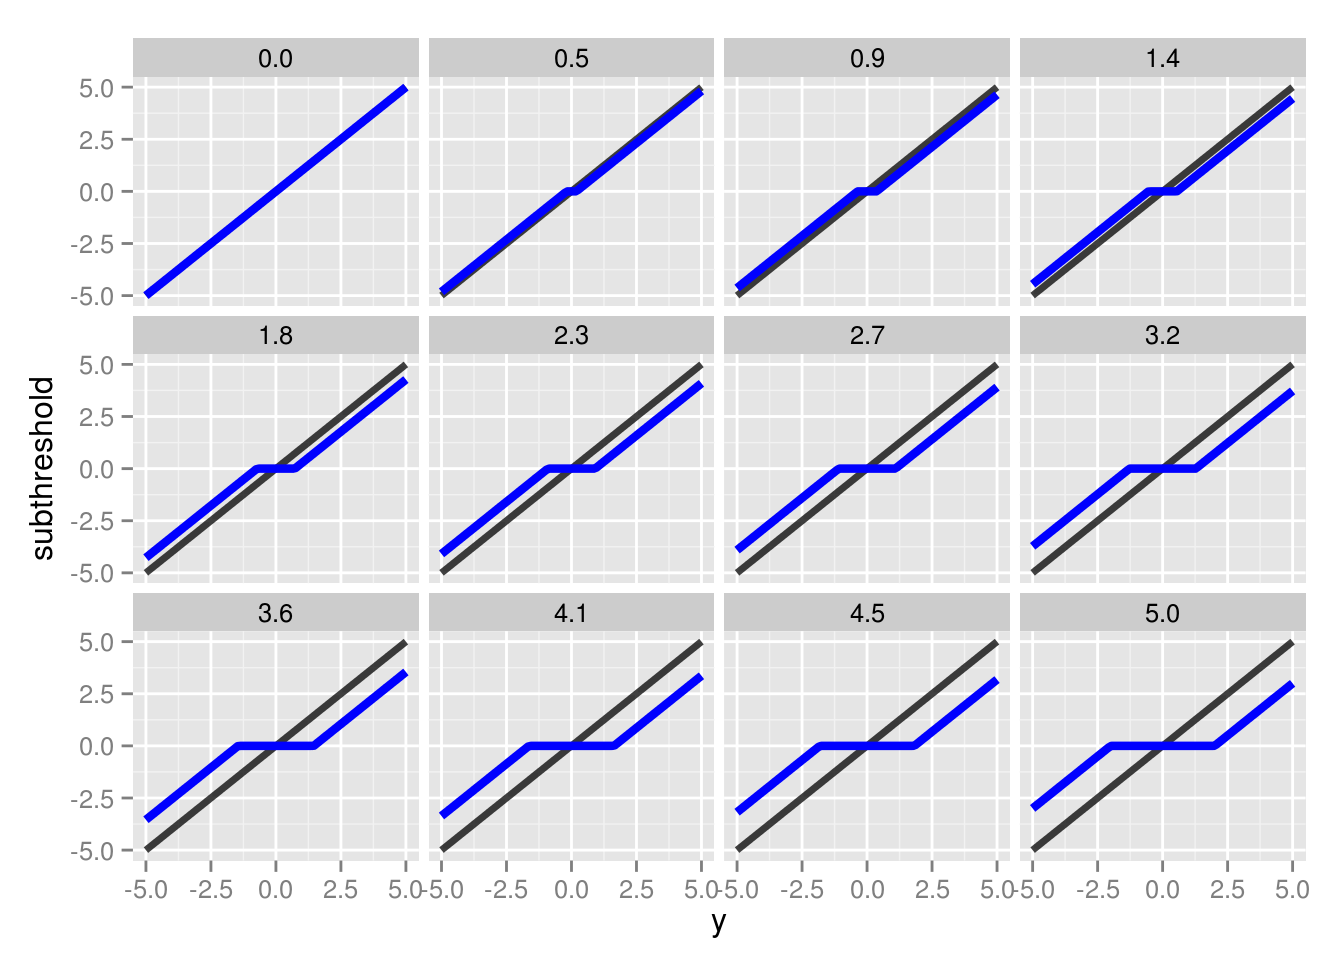
\includegraphics{figs/lasso/1.png}
\caption{}
\end{figure}

The value of \(y_j\) is represented by the black lines, whereas the
subthresholding transformation is represented by the blue lines. For
values outside of the \(|y_j|\) interval, the function essentially
drives \(y_j\) closer to 0. Once it's within that interval, \(y_j\) is
\emph{set} to zero. The size of this interval is determined by
\(\lambda\), with larger values producing a larger interval, and
consequently, a more sparse solution.

\subsection{Multivariate Lasso
Regression}\label{multivariate-lasso-regression}

In the multivariate case, the lasso problem becomes
\[\underset{\beta}{\mathrm{min}} \frac{1}{2} ||y-X\beta||_2^2 + \lambda ||\beta||_1\],
which can only be solved explicitly if \(X^TX=I\), a case that isn't met
when \(p>n\). Coordinate descent provides a solution for the
multivariate regression problem. Here, the subthresholding function
becomes:

\[
  \hat \beta_j = \left\{\def\arraystretch{1.2}%
  \begin{array}{@{}c@{\quad}l@{}}
    c_j - p\lambda/a_j & \text{if $c_j > p\lambda$}\\
    c_j + p\lambda/a_j & \text{if $c_j < - p\lambda$}\\
    0                  & \text{if $|c_j| \le p\lambda$}\\
  \end{array}\right.
\]

where p is the dimensionality of the feature vector. Because it's easier
to optimize each \(jth\) coefficient individually, instead of solving
for the entire feature vector simultaneously, we solve for the \(jth\)
coefficient while holding all others fixed. This results in
\(c_j = X_{\cdot,j}^T(y - X_{\cdot,-j}\beta_{-j})\) and
\(a_j = \sum_{i=1}^n x_{i,-j}\). This is often performed sequentially,
i.e., for each iteration each \(\beta\) is updated, one-by-one. This is
called the shooting algorithm. A slight adjustment allows for easy
parallel implementation.

\subsection{Parallel Coordinate
Descent}\label{parallel-coordinate-descent}

Unlike before where each \(\beta_j\) is updated during each iteration
until convergence, an alternative strategy is to randomly sample index
\(j\) to update during each iteration. While this method would require
more iterations, each iteration will be faster, and it will still
ultimately converge. Because the \(jth\) index is now being sampled, an
obvious extension is to simply distribute a randomly sampled index to
each of m processors on a cluster. Each processor can than update its
respective \(\beta_j\) independently, resulting in m simultaneous
updates per iteration.

This requires a rather simple implementation via MPI. Set vector
\textbf{B} of length p to 0. Given m processors, m indexes are drawn
from a uniform distribution ranging 1 to m. This index vector is then
sent to each processor via MPI\_Scatter. Each processor independently
updates \(a_j\), \(c_j\), and ultimately \(\beta_j\). The updated
\(\beta_j\)s are then returned to the head node using MPI\_gather, where
the original vector \textbf{B} is then updated and then distributed
across all processes with MPI\_bcast for future iterations. This is
repeated until convergence -- i.e., when two sequential iterations
result in a change of the objective function less than a predetermined
tolerance value. The objective function function is defined as
\[\frac{1}{2m} ||y-X\beta||_2^2 + \lambda \sum_{i=1}^n |\beta|\].

\subsection{Simulations}\label{simulations}

All matrices were generated as follows: X, a \(m \times n\) matrix, and
k \(\beta\) values were sampled from a normal distribution (0,1). The k
\(\beta\) values were set to k randomly sampled indexes sampled from a
uniform distribution (1,n) in a \(m \times 1\) vector \beta. All other
values were set to 0. Finally, y was calculated via \(y = X^T b\).

\subsubsection{\texorpdfstring{\(50 \times 1000\) Matrix \textbar{} 5
Target
Coefficients}{50 \textbackslash{}times 1000 Matrix \textbar{} 5 Target Coefficients}}\label{times-1000-matrix-5-target-coefficients}

Before any analysis of the results was performed, there seemed to be
numerical issues when performing the algorithm on small \(\lambda\)
values (\(<.05\)). The objective and all \(\beta\) coefficients would
increase exponentially after every update. Only with larger \(\lambda\)
values would the algorithm converge (and note it would always converge
to the correct values). It turned out this was unrelated to the code;
there were no errors. Instead, it was a function of the number of cores
set. All initial runs were performed with 64 cores, resulting in the
numerical issue for small \(\lambda\) values. Note that this is neither
an MPI problem nor a problem inherent to the cluster. The issue lies in
selecting more simultaneous updates than there is data (rows in matrix
X), which, in this simulation, there are 50. See the figure below:

\begin{figure}[htbp]
\centering
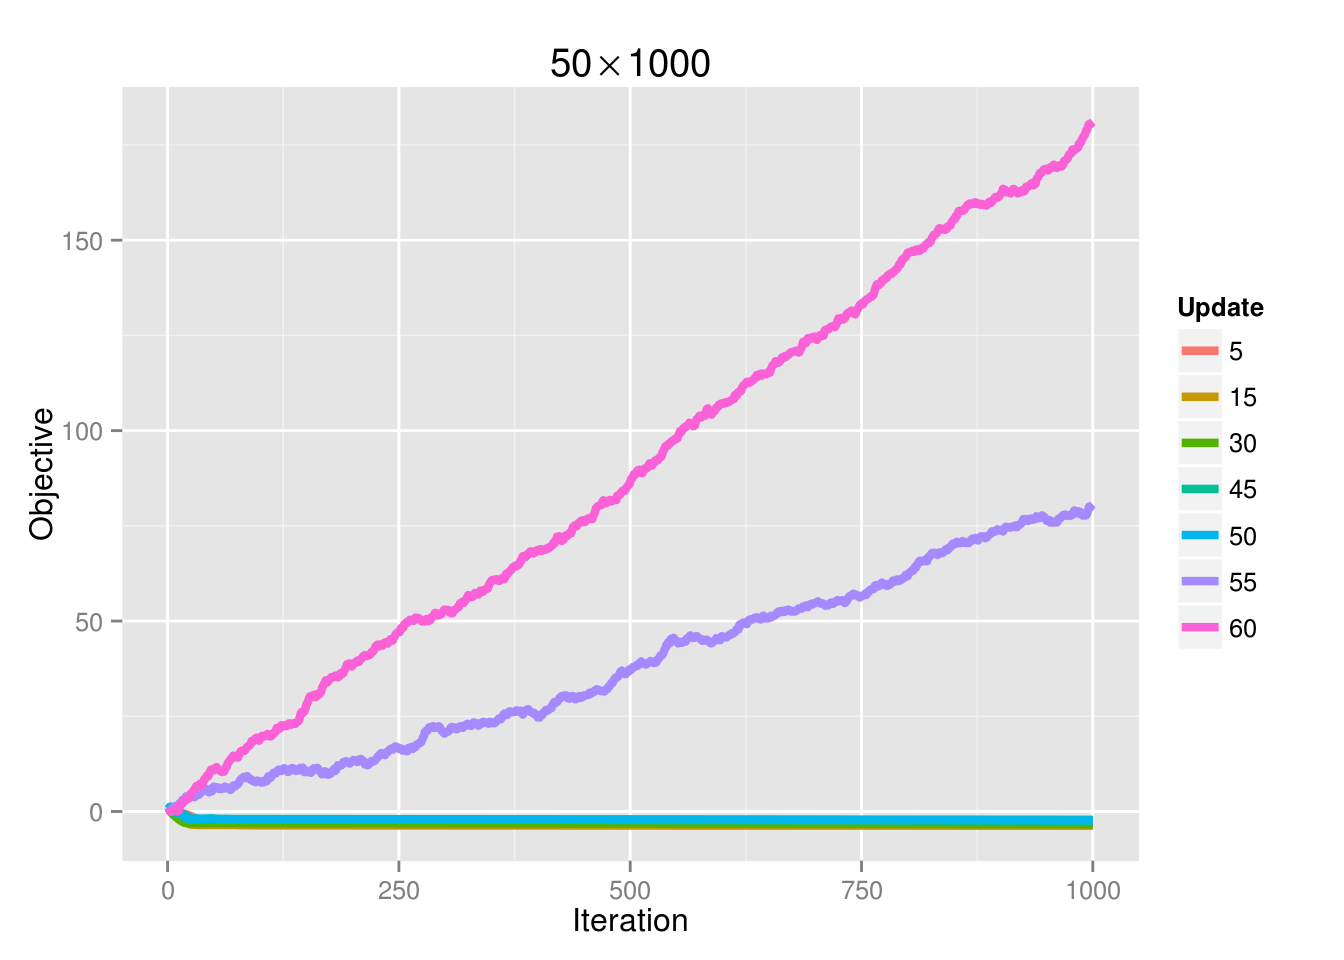
\includegraphics{figs/lasso/2.png}
\caption{}
\end{figure}

If we increase the sample size to 100, then the convergence problem is
gone:

\begin{figure}[htbp]
\centering
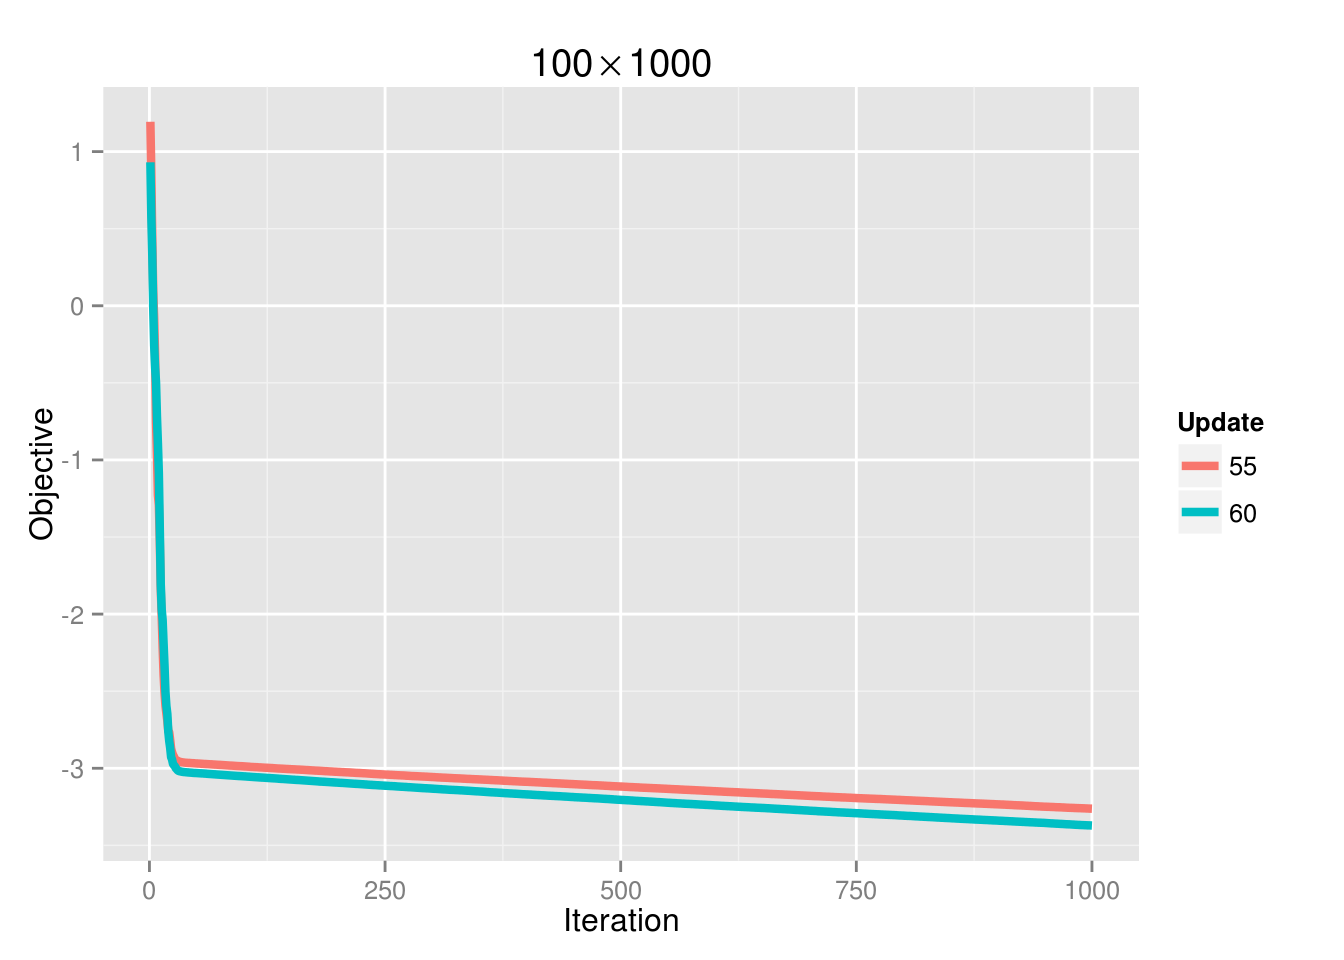
\includegraphics{figs/lasso/3.png}
\caption{}
\end{figure}

And the ability to achieve convergence as a function of processors is
also dictated by \(\lambda\):

\begin{figure}[htbp]
\centering
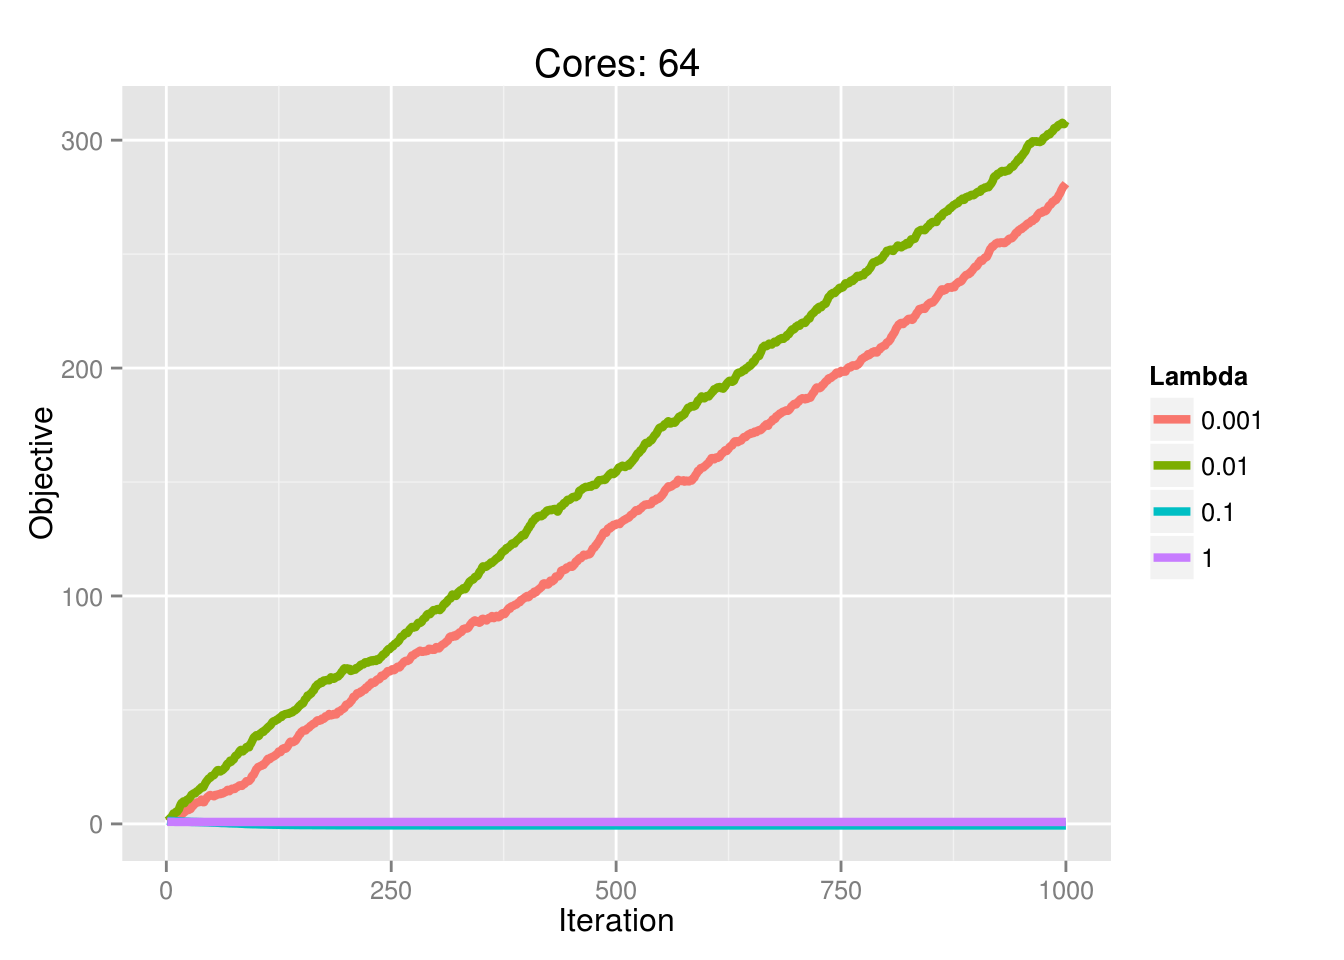
\includegraphics{figs/lasso/4.png}
\caption{}
\end{figure}

Here are the lasso traces for 10 independent samples for the above
parameter settings

\begin{figure}[htbp]
\centering
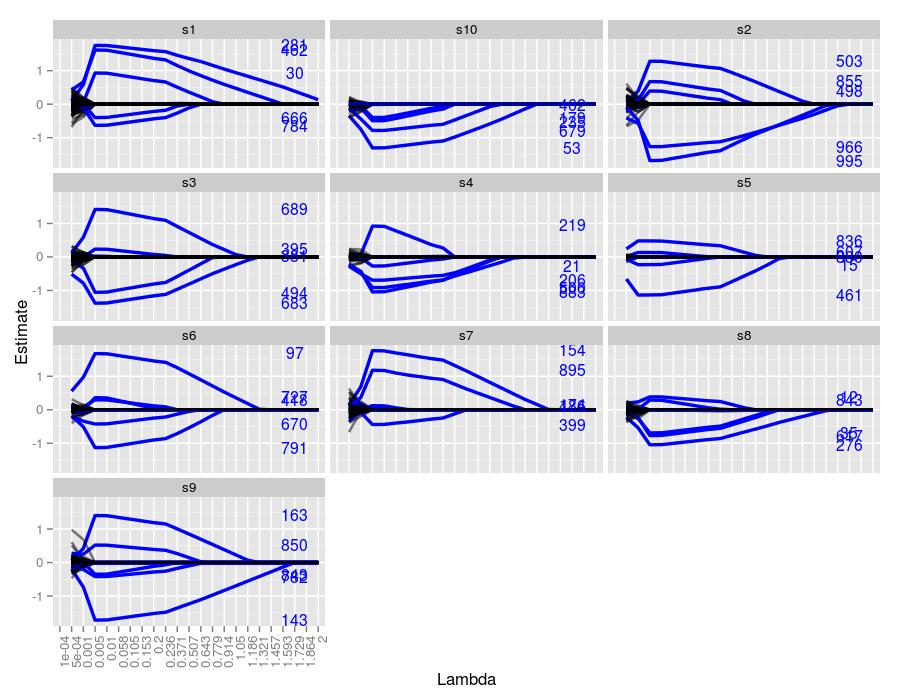
\includegraphics{figs/lasso/5.jpg}
\caption{}
\end{figure}

The text on the right hand side represents the indexes of the true
coefficients used to generate the system for each sample. Their height
represents their true value. We can easily see which traces correspond
to which index, and moreover, we can see the \(\lambda\) value in which
the traces achieve the correct value. Every sample managed to both
identify and estimate the correct index and its coefficient at some
point throughout the trace. The figures seem to suggest that
\(\lambda=-.005\) did the best job at estimating the true values.
Coefficients with larger values were more robust to smaller \(\lambda\)
values. For example, in sample 7, coefficients 154 and 895 were nonzero
for \(\lambda\) values well over 1. Coefficient 399 was driven to zero
around \(\lambda=.5\), whereas the remaining two coefficients were set
to 0 much sooner.

Here is the error at each \(\lambda\) averaged across samples:

\begin{figure}[htbp]
\centering
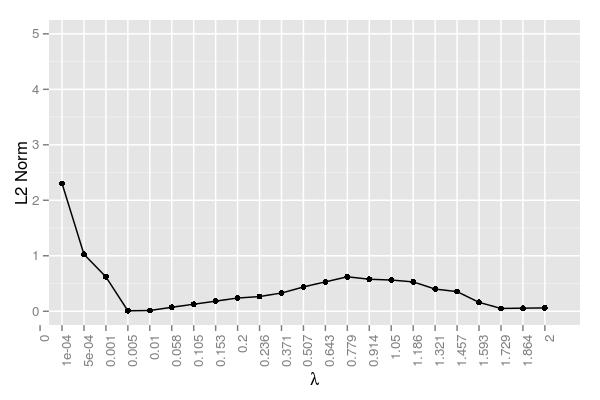
\includegraphics{figs/lasso/6.jpg}
\caption{}
\end{figure}

The error term here is measured as the following:
\[\mathrm{Error}=\frac{||\hat x - x||_2}{||x||_2}\]. This figure
confirms \(\lambda=.005\) performing the best. It should be noted that
there was an iteration cap, so the very small \(\lambda\) values likely
just failed to reach a reasonable approximation. While they clearly were
converging and hence approaching a reasonable solution, it simply would
have taken too long and these values were the result of 20,000
iterations using 48 cores. The error began to rise somewhat around
\(\lambda=.779\) The hump in this region and the subsequent decline can
be attributed to the variability regarding when certain coefficients are
driven to 0. Samples 1 and 2 have a few relatively robust coefficients
that help decrease the error, whereas the coefficients in sample 4 are
probably key contributors in the hump around \(\lambda=.779\).

\subsubsection{\texorpdfstring{\(50 \times 10000\) Matrix \textbar{} 5
Target
Coefficients}{50 \textbackslash{}times 10000 Matrix \textbar{} 5 Target Coefficients}}\label{times-10000-matrix-5-target-coefficients}

\begin{figure}[htbp]
\centering
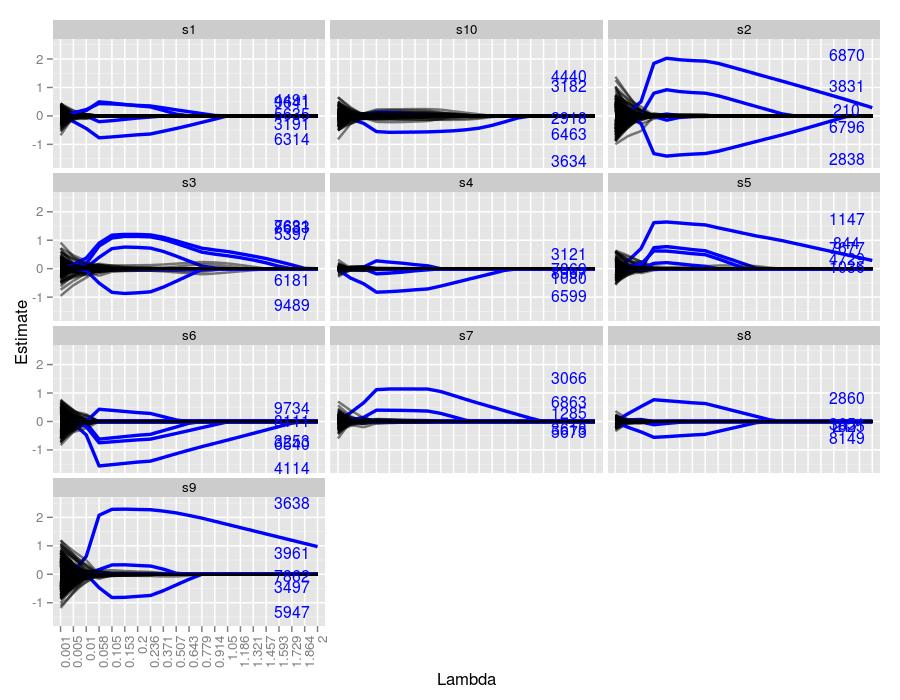
\includegraphics{figs/lasso/7.jpg}
\caption{}
\end{figure}

Now we are dealing with 10 times more unwanted coefficients, and the
figures make it quite obvious that lasso is having more trouble than the
\(50 \times 1000\) case. Sample 10 managed to capture only 1 coefficient
for a prolonged stretch, and it also had quite a few false positives for
moderate \(\lambda\) values. Sample 3 also had quite a few false
positives, but farther along than sample 10. Samples 7 and 8 detected
only 2 of the 5 coefficients. Like the previous simulation, larger true
coefficients were more robust at being detected across \(\lambda\)
values, exemplified quite well by sample 2.

\begin{figure}[htbp]
\centering
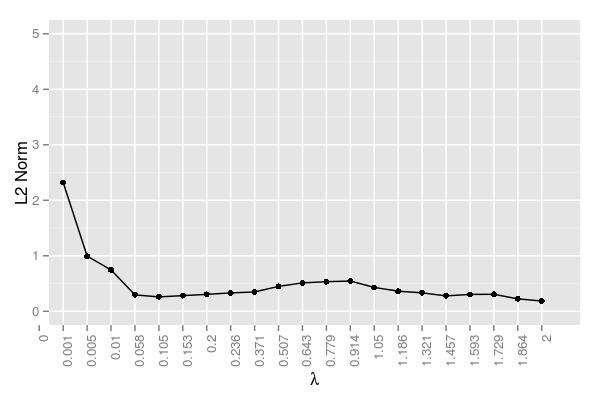
\includegraphics{figs/lasso/8.jpg}
\caption{}
\end{figure}

Unlike the last simulation, \(\lambda=.005\) performed poorly. The best
value seemed to be around \(\lambda=.058\), although each value ranging
from .058 to .371 did quite well. Still, even for .058, the error was
larger (approximately .300) than .005 (.009) for the last simulation

\subsubsection{\texorpdfstring{\(200 \times 10000\) Matrix \textbar{} 5
Target
Coefficients}{200 \textbackslash{}times 10000 Matrix \textbar{} 5 Target Coefficients}}\label{times-10000-matrix-5-target-coefficients-1}

\begin{figure}[htbp]
\centering
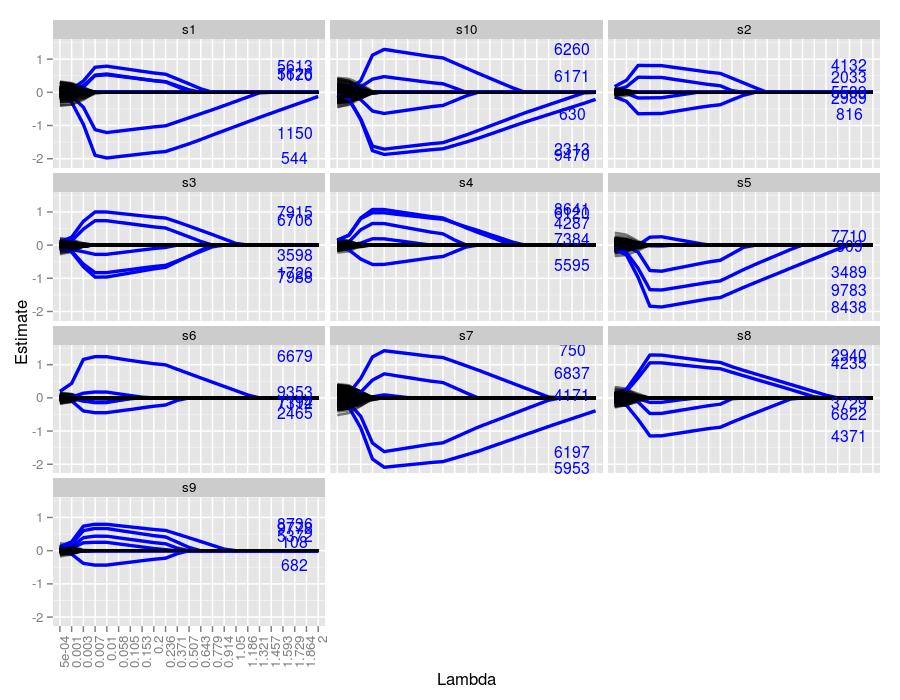
\includegraphics{figs/lasso/9.jpg}
\caption{}
\end{figure}

By increasing the number of data points from 50 to 200, there seems to
be a return to the behavior we saw in the \(50 \times 1000\) simulation.
Notwithstanding sample 6, all of the samples managed to estimate at
least 4 of the 5 coefficients. Again, if the coefficient was truly
large, then it behaved robustly across all \(\lambda\) values.

\begin{figure}[htbp]
\centering
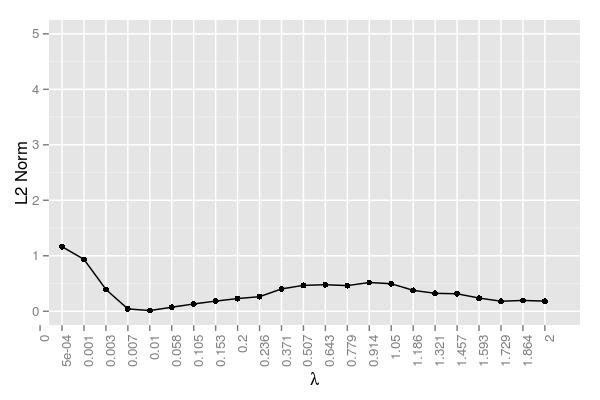
\includegraphics{figs/lasso/10.jpg}
\caption{}
\end{figure}

The error too seems similar to the \(50 \times 1000\) simulation. The
minimum ended up being at \(\lambda=0.007\), analogous to the minimum of
.005 we saw in the smaller system. The error managed to stay low even
for a slightly larger \(\lambda\) (.01). Like all of the simulations so
far, there is a hump at the moderate \(\lambda\) values.

Based on the last 3 simulations, there seems to be a trade-off between
the amount of data (i.e., the number of rows in \(X\)) and the number of
coefficients (i.e., the columns in \(X\)). More coefficients gives lasso
problems, but given more data, then lasso returns to form. Let's see how
lasso does at estimating more coefficients.

\subsubsection{\texorpdfstring{\(50 \times 10000\) Matrix \textbar{} 15
Target
Coefficients}{50 \textbackslash{}times 10000 Matrix \textbar{} 15 Target Coefficients}}\label{times-10000-matrix-15-target-coefficients}

\begin{figure}[htbp]
\centering
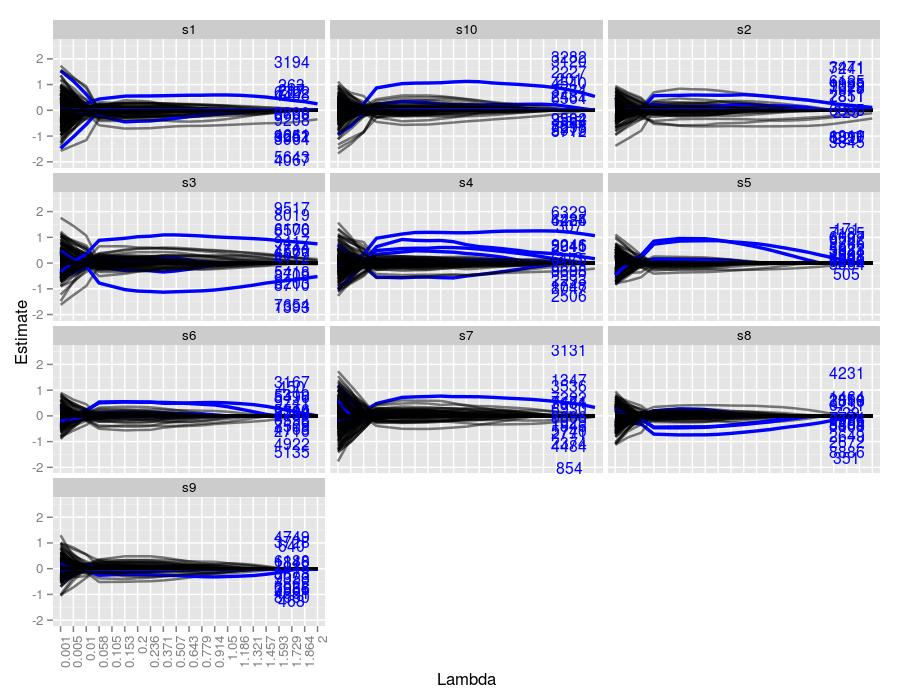
\includegraphics{figs/lasso/11.jpg}
\caption{}
\end{figure}

Now lasso seems to be struggling to find the true coefficients. Other
than sample 4, which managed to only capture about 6 of the 15
coefficients, all of the samples performed poorly. Other than a few
large coefficients, most traces were lost in false positives. Also,
unlike the systems with only 5 true coefficients, this simulation
resulted in many incorrect traces of similar magnitude to the true
coefficients, represented by the black lines. It's surprising that lasso
even failed to capture the larger coefficients (see the labels far from
the x-axis). The fact that there are quite a few coefficients not much
larger than 0 in terms of magnitude (recall they are sampled from a
normal distribution (0,1)) gives lasso problems setting any potentially
non-zero coefficient to zero. This may be remedied by a smaller
tolerance, but most likely, it won't make a difference. For example,
with \(\lambda=2.\) (sample 4), the tolerance level was reached after
only 1999 iterations, managing only to capture 4 coefficients, all of
which are far smaller in magnitude than their true counterparts. A
smaller \(\lambda\) of 0.01 (sample 10) reached the iteration cap of
20,000, but ended up with 317 coefficients, far more than the target 15.
A more moderate value, \(\lambda=1.05\) (sample 1), broke after 5499
iterations, ending with 21 coefficients, which is closer to 15, but
nevertheless failed to capture any of the true estimates of the larger
coefficients since no trace reaches the required height.

\begin{figure}[htbp]
\centering
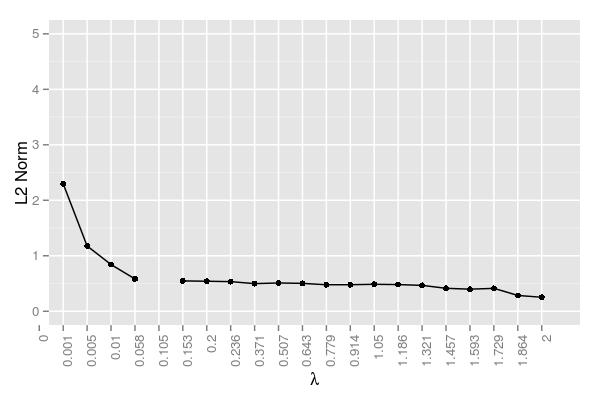
\includegraphics{figs/lasso/12.jpg}
\caption{}
\end{figure}

Note the gap in the plot was due to the aforementioned convergence/core
issue; hence, those \(\lambda\) values were omitted. The error here
essentially reaches a plateau for the majority of the \(\lambda\)
values. The error drops at the end, but this is not due to improved
estimation, but instead a result of driving many of the incorrect
estimates to zero.

Considering this situation, if one has a dataset with many potentially
informative coefficients, unless some yield significantly large
estimates relative to the majority, then lasso will likely have
problems. Since this simulation dealt with true coefficients near 0,
many false positives resulted. A noisy dataset probably requires the use
of larger \(\lambda\) values and the hope that the some coefficients are
significantly more informative than the others.

\subsubsection{\texorpdfstring{\(50 \times 10000\) Matrix \textbar{} 30
Target
Coefficients}{50 \textbackslash{}times 10000 Matrix \textbar{} 30 Target Coefficients}}\label{times-10000-matrix-30-target-coefficients}

\begin{figure}[htbp]
\centering
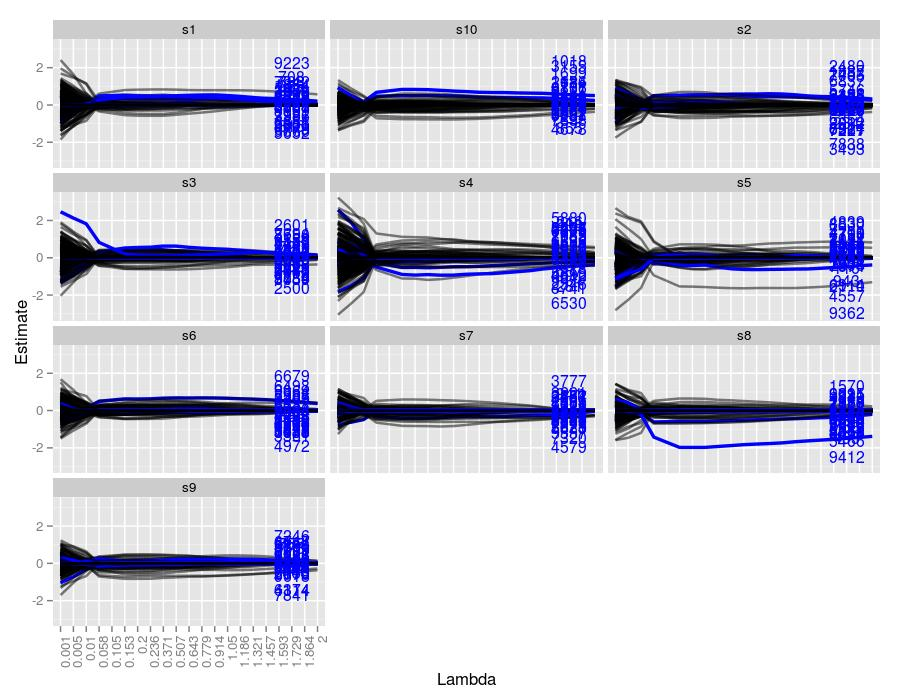
\includegraphics{figs/lasso/13.jpg}
\caption{}
\end{figure}

And here's an even noisier system, with 30 true coefficients. Only
sample 8 was able to separate a coefficient from the crown. Driving
\(\lambda\) up further for this sample would likely isolate it. Sample 5
also had a large robust estimate, but it was a false positive. Clearly
the conclusion reached in the last simulation can only be confirmed
here.

\begin{figure}[htbp]
\centering
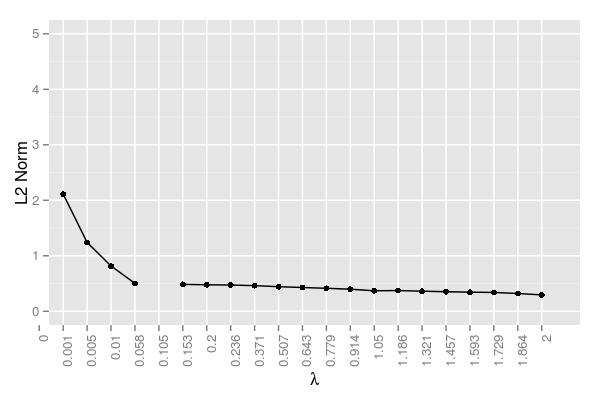
\includegraphics{figs/lasso/14.jpg}
\caption{}
\end{figure}

The trend here is similar to the system with 15 true values. If we
increase \(\lambda\) further, we would likely see the same drop in error
we see before since we'd be driving the many incorrect estimates to
zero.

\subsubsection{Scaling the coeficients}\label{scaling-the-coeficients}

It seems plausible that as we increase the number of false coefficients,
we decrease the chance of identifying true coefficients unless those
coefficients are much different than the majority -- i.e., more
informative. Instead of increasing the sampling size this time, let's
increase the magnitude of the true coefficients by scaling them 10-fold.
Using a \emph{very} large \(50 \times 100000\) matrix, we get the
following:

\begin{figure}[htbp]
\centering
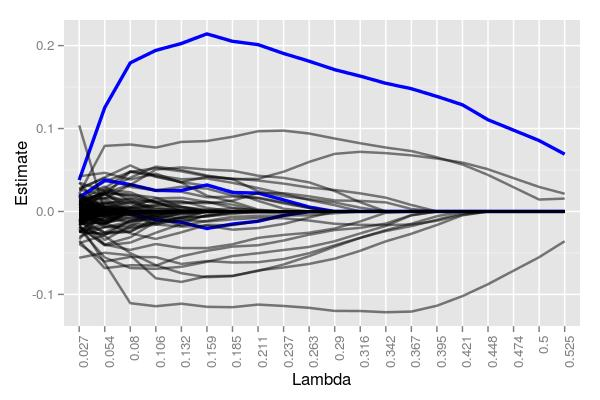
\includegraphics{figs/lasso/15.jpg}
\caption{}
\end{figure}

Even with 100,000 potential coefficients to work with, lasso managed to
cleanly identify one of the five targets. Moreover, while there are
quite a few false positives around \(\lambda=.211\) (30), there are
\emph{far} less than 100,000, and 3 total true coefficients were still
detectable. At \(\lambda=.525\), 4 coefficients were returned, albeit
only 1 being correct. Had we used larger \(\lambda\) values, we likely
would have ended with at most 1 true and 1 false coefficient. Note that
the 5 starting coefficients had values of -4.79, 9.88, 3.12, 1.22, and
7.02. That robust coefficient was, to no one's surprise, the coefficient
with the largest value in magnitude of the 5, 9.88.

\subsubsection{Comparison}\label{comparison}

\begin{figure}[htbp]
\centering
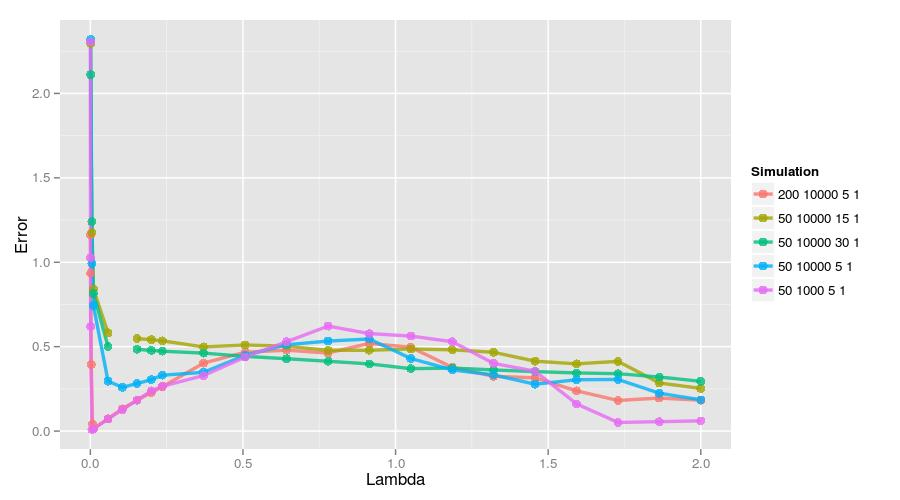
\includegraphics{figs/lasso/16.jpg}
\caption{}
\end{figure}

Here is a figure showing all of the error traces. The small system
(\(50 \times 1000\)) and the large system with more data
(\(200 \times 10000\)) performed the best assuming a small \(\lambda\)
was used. Interestingly, if only uses a larger \(\lambda\), then that
small system tends to perform the worst. Still, it's quite clear that
identifying informative features is a function of the amount of data,
the number of features, the number of true coefficients, and their size.

\subsection{Conclusion}\label{conclusion}

A parallelized implementation of the coordinate descent algorithm for
lasso clearly works well for large datasets. The issue with cores and
the number of rows is an interesting quirk, but nevertheless easily
avoidable. Once that was accounted for, no numerical issues resulted,
and estimates were consistent with the predetermined values designed for
the simulations.

\begin{Shaded}
\begin{Highlighting}[]
\NormalTok{y <-}\StringTok{ }\NormalTok{Boston$medv }\CommentTok{# median housing value}
\NormalTok{X <-}\StringTok{ }\KeywordTok{as.matrix}\NormalTok{(Boston[,-}\DecValTok{14}\NormalTok{]) }\CommentTok{# all other predictors}

\NormalTok{y <-}\StringTok{ }\KeywordTok{scale}\NormalTok{(y,}\DataTypeTok{center=}\OtherTok{TRUE}\NormalTok{,}\DataTypeTok{scale=}\OtherTok{FALSE}\NormalTok{)}
\NormalTok{X <-}\StringTok{ }\KeywordTok{scale}\NormalTok{(X,}\DataTypeTok{center =} \OtherTok{TRUE}\NormalTok{,}\DataTypeTok{scale =} \OtherTok{FALSE}\NormalTok{)}

\NormalTok{B <-}\StringTok{ }\KeywordTok{rep}\NormalTok{(}\DecValTok{0}\NormalTok{,}\KeywordTok{ncol}\NormalTok{(X))}
\NormalTok{lambda <-}\StringTok{ }\DecValTok{2}
\NormalTok{tol <-}\StringTok{ }\FloatTok{1e-8}
\NormalTok{m <-}\StringTok{ }\KeywordTok{length}\NormalTok{(y)}

\NormalTok{iter <-}\StringTok{ }\DecValTok{1000}

\NormalTok{obj <-}\StringTok{ }\KeywordTok{numeric}\NormalTok{(iter +}\StringTok{ }\DecValTok{1}\NormalTok{)}
\NormalTok{B.list <-}\StringTok{ }\KeywordTok{lapply}\NormalTok{(}\DecValTok{1}\NormalTok{:(iter +}\StringTok{ }\DecValTok{1}\NormalTok{), function(x) x)}
\NormalTok{B.list[[}\DecValTok{1}\NormalTok{]] <-}\StringTok{ }\NormalTok{B}

\NormalTok{for (j in }\DecValTok{1}\NormalTok{:iter) \{}
  
  \NormalTok{k <-}\StringTok{ }\KeywordTok{sample}\NormalTok{(}\DecValTok{1}\NormalTok{:}\KeywordTok{length}\NormalTok{(B),}\DecValTok{1}\NormalTok{)}
  
  \CommentTok{# 0 for B0 but centered so 0}
  \CommentTok{# calculate Bj for for all j not in k}

  \NormalTok{cj <-}\StringTok{ }\NormalTok{(X[,k] %*%}\StringTok{ }\NormalTok{(y -}\StringTok{ }\NormalTok{X[,-k] %*%}\StringTok{ }\NormalTok{B[-k])) }\CommentTok{# *2}
  \NormalTok{aj <-}\StringTok{ }\KeywordTok{sum}\NormalTok{(X[,k]^}\DecValTok{2}\NormalTok{)  }\CommentTok{# *2}
  
  \CommentTok{# shrink}
  \NormalTok{Bj <-}\StringTok{ }\DecValTok{0}
  \NormalTok{if (cj <}\StringTok{ }\NormalTok{-lambda*m) Bj <-}\StringTok{ }\NormalTok{(cj +}\StringTok{ }\NormalTok{lambda*m)/aj}
  \NormalTok{if (cj >}\StringTok{ }\NormalTok{lambda*m) Bj <-}\StringTok{ }\NormalTok{(cj -}\StringTok{ }\NormalTok{lambda*m)/aj}

  \NormalTok{B[k] <-}\StringTok{ }\NormalTok{Bj}
  
  \NormalTok{B.list[[(j +}\StringTok{ }\DecValTok{1}\NormalTok{)]] <-}\StringTok{ }\NormalTok{B}
  \NormalTok{obj[j] <-}\StringTok{ }\NormalTok{(}\DecValTok{1}\NormalTok{/}\DecValTok{2}\NormalTok{)*(}\DecValTok{1}\NormalTok{/m)*}\KeywordTok{norm}\NormalTok{(y -}\StringTok{ }\NormalTok{X %*%}\StringTok{ }\NormalTok{B,}\StringTok{"F"}\NormalTok{)^}\DecValTok{2} \NormalTok{+}\StringTok{ }\NormalTok{lambda*}\KeywordTok{sum}\NormalTok{(}\KeywordTok{abs}\NormalTok{(B))}
  
  \CommentTok{#if (sqrt(sum((B.list[[j]] - B.list[[j+1]])^2)) < tol) break}
\NormalTok{\} }

\NormalTok{g <-}\StringTok{ }\NormalTok{(}\DecValTok{1}\NormalTok{/m)*}\KeywordTok{t}\NormalTok{(X) %*%}\StringTok{ }\NormalTok{(y -}\StringTok{ }\NormalTok{X %*%}\StringTok{ }\NormalTok{B)}
\NormalTok{if (}\KeywordTok{any}\NormalTok{(}\KeywordTok{abs}\NormalTok{(g[}\KeywordTok{which}\NormalTok{(B ==}\StringTok{ }\DecValTok{0}\NormalTok{)]) >}\StringTok{ }\NormalTok{lambda +}\StringTok{ }\NormalTok{tol)) }\KeywordTok{print}\NormalTok{(}\StringTok{"No minimum"}\NormalTok{)}
\NormalTok{if (}\KeywordTok{any}\NormalTok{(g[}\KeywordTok{which}\NormalTok{(B !=}\StringTok{ }\DecValTok{0}\NormalTok{)] >}\StringTok{ }\NormalTok{tol +}\StringTok{ }\NormalTok{lambda*}\KeywordTok{sign}\NormalTok{(B[}\KeywordTok{which}\NormalTok{(B !=}\StringTok{ }\DecValTok{0}\NormalTok{)]))) }\KeywordTok{print}\NormalTok{(}\StringTok{"No minimum"}\NormalTok{)}
\end{Highlighting}
\end{Shaded}

\begin{verbatim}
## [1] "No minimum"
\end{verbatim}

\begin{Shaded}
\begin{Highlighting}[]
\NormalTok{B}
\end{Highlighting}
\end{Shaded}

\begin{verbatim}
##  [1] -0.021552320294  0.035523120761  0.000000000000  0.000000000000
##  [5]  0.000000000000  0.000000000000  0.043564050481 -0.067585897623
##  [9]  0.173365654135 -0.011672463466 -0.557109230058  0.007065846342
## [13] -0.821549115759
\end{verbatim}

\subsection{Code: Lasso}\label{code-lasso}

\begin{Shaded}
\begin{Highlighting}[]
\NormalTok{y <-}\StringTok{ }\NormalTok{Boston$medv }\CommentTok{# median housing value}
\NormalTok{X <-}\StringTok{ }\KeywordTok{as.matrix}\NormalTok{(Boston[,-}\DecValTok{14}\NormalTok{]) }\CommentTok{# all other predictors}

\NormalTok{y <-}\StringTok{ }\KeywordTok{scale}\NormalTok{(y,}\DataTypeTok{center=}\OtherTok{TRUE}\NormalTok{,}\DataTypeTok{scale=}\OtherTok{FALSE}\NormalTok{)}
\NormalTok{X <-}\StringTok{ }\KeywordTok{scale}\NormalTok{(X,}\DataTypeTok{center =} \OtherTok{TRUE}\NormalTok{,}\DataTypeTok{scale =} \OtherTok{FALSE}\NormalTok{)}

\NormalTok{B <-}\StringTok{ }\KeywordTok{rep}\NormalTok{(}\DecValTok{0}\NormalTok{,}\KeywordTok{ncol}\NormalTok{(X))}
\NormalTok{lambda <-}\StringTok{ }\DecValTok{2}
\NormalTok{tol <-}\StringTok{ }\FloatTok{1e-8}
\NormalTok{m <-}\StringTok{ }\KeywordTok{length}\NormalTok{(y)}

\NormalTok{iter <-}\StringTok{ }\DecValTok{1000}

\NormalTok{obj <-}\StringTok{ }\KeywordTok{numeric}\NormalTok{(iter +}\StringTok{ }\DecValTok{1}\NormalTok{)}
\NormalTok{B.list <-}\StringTok{ }\KeywordTok{lapply}\NormalTok{(}\DecValTok{1}\NormalTok{:(iter +}\StringTok{ }\DecValTok{1}\NormalTok{), function(x) x)}
\NormalTok{B.list[[}\DecValTok{1}\NormalTok{]] <-}\StringTok{ }\NormalTok{B}

\NormalTok{for (j in }\DecValTok{1}\NormalTok{:iter) \{}
  
  \NormalTok{k <-}\StringTok{ }\KeywordTok{sample}\NormalTok{(}\DecValTok{1}\NormalTok{:}\KeywordTok{length}\NormalTok{(B),}\DecValTok{1}\NormalTok{)}
  
  \CommentTok{# 0 for B0 but centered so 0}
  \CommentTok{# calculate Bj for for all j not in k}

  \NormalTok{cj <-}\StringTok{ }\NormalTok{(X[,k] %*%}\StringTok{ }\NormalTok{(y -}\StringTok{ }\NormalTok{X[,-k] %*%}\StringTok{ }\NormalTok{B[-k])) }\CommentTok{# *2}
  \NormalTok{aj <-}\StringTok{ }\KeywordTok{sum}\NormalTok{(X[,k]^}\DecValTok{2}\NormalTok{)  }\CommentTok{# *2}
  
  \CommentTok{# shrink}
  \NormalTok{Bj <-}\StringTok{ }\DecValTok{0}
  \NormalTok{if (cj <}\StringTok{ }\NormalTok{-lambda*m) Bj <-}\StringTok{ }\NormalTok{(cj +}\StringTok{ }\NormalTok{lambda*m)/aj}
  \NormalTok{if (cj >}\StringTok{ }\NormalTok{lambda*m) Bj <-}\StringTok{ }\NormalTok{(cj -}\StringTok{ }\NormalTok{lambda*m)/aj}

  \NormalTok{B[k] <-}\StringTok{ }\NormalTok{Bj}
  
  \NormalTok{B.list[[(j +}\StringTok{ }\DecValTok{1}\NormalTok{)]] <-}\StringTok{ }\NormalTok{B}
  \NormalTok{obj[j] <-}\StringTok{ }\NormalTok{(}\DecValTok{1}\NormalTok{/}\DecValTok{2}\NormalTok{)*(}\DecValTok{1}\NormalTok{/m)*}\KeywordTok{norm}\NormalTok{(y -}\StringTok{ }\NormalTok{X %*%}\StringTok{ }\NormalTok{B,}\StringTok{"F"}\NormalTok{)^}\DecValTok{2} \NormalTok{+}\StringTok{ }\NormalTok{lambda*}\KeywordTok{sum}\NormalTok{(}\KeywordTok{abs}\NormalTok{(B))}
  
  \CommentTok{#if (sqrt(sum((B.list[[j]] - B.list[[j+1]])^2)) < tol) break}
\NormalTok{\} }

\NormalTok{g <-}\StringTok{ }\NormalTok{(}\DecValTok{1}\NormalTok{/m)*}\KeywordTok{t}\NormalTok{(X) %*%}\StringTok{ }\NormalTok{(y -}\StringTok{ }\NormalTok{X %*%}\StringTok{ }\NormalTok{B)}
\NormalTok{if (}\KeywordTok{any}\NormalTok{(}\KeywordTok{abs}\NormalTok{(g[}\KeywordTok{which}\NormalTok{(B ==}\StringTok{ }\DecValTok{0}\NormalTok{)]) >}\StringTok{ }\NormalTok{lambda +}\StringTok{ }\NormalTok{tol)) }\KeywordTok{print}\NormalTok{(}\StringTok{"No min"}\NormalTok{)}
\NormalTok{if (}\KeywordTok{any}\NormalTok{(g[}\KeywordTok{which}\NormalTok{(B !=}\StringTok{ }\DecValTok{0}\NormalTok{)] >}\StringTok{ }\NormalTok{tol +}\StringTok{ }\NormalTok{lambda*}\KeywordTok{sign}\NormalTok{(B[}\KeywordTok{which}\NormalTok{(B !=}\StringTok{ }\DecValTok{0}\NormalTok{)]))) }\KeywordTok{print}\NormalTok{(}\StringTok{"No min"}\NormalTok{)}
\end{Highlighting}
\end{Shaded}

\begin{verbatim}
## [1] "No min"
\end{verbatim}

\begin{Shaded}
\begin{Highlighting}[]
\NormalTok{B}
\end{Highlighting}
\end{Shaded}

\begin{verbatim}
##  [1] -0.02157812903  0.03552762001  0.00000000000  0.00000000000  0.00000000000
##  [6]  0.00000000000  0.04356367353 -0.06769672154  0.17352502255 -0.01168198944
## [11] -0.55710594088  0.00706537907 -0.82151479590
\end{verbatim}

\subsection{Code: Lasso via cyclic gradient
descent}\label{code-lasso-via-cyclic-gradient-descent}

\begin{Shaded}
\begin{Highlighting}[]
\NormalTok{y <-}\StringTok{ }\NormalTok{Boston$medv }\CommentTok{# median housing value}
\NormalTok{X <-}\StringTok{ }\KeywordTok{as.matrix}\NormalTok{(Boston[,-}\DecValTok{14}\NormalTok{]) }\CommentTok{# all other predictors}

\NormalTok{y <-}\StringTok{ }\KeywordTok{scale}\NormalTok{(y,}\DataTypeTok{center=}\OtherTok{TRUE}\NormalTok{,}\DataTypeTok{scale=}\OtherTok{FALSE}\NormalTok{)}
\NormalTok{X <-}\StringTok{ }\KeywordTok{scale}\NormalTok{(X,}\DataTypeTok{center =} \OtherTok{TRUE}\NormalTok{,}\DataTypeTok{scale =} \OtherTok{FALSE}\NormalTok{)}

\NormalTok{B <-}\StringTok{ }\KeywordTok{rep}\NormalTok{(}\DecValTok{0}\NormalTok{,}\KeywordTok{ncol}\NormalTok{(X))}
\NormalTok{lambda <-}\StringTok{ }\DecValTok{2}
\NormalTok{tol <-}\StringTok{ }\FloatTok{1e-8}
\NormalTok{m <-}\StringTok{ }\KeywordTok{length}\NormalTok{(y)}

\NormalTok{iter <-}\StringTok{ }\DecValTok{500}

\NormalTok{obj <-}\StringTok{ }\KeywordTok{numeric}\NormalTok{(iter +}\StringTok{ }\DecValTok{1}\NormalTok{)}
\NormalTok{B.list <-}\StringTok{ }\KeywordTok{lapply}\NormalTok{(}\DecValTok{1}\NormalTok{:(iter +}\StringTok{ }\DecValTok{1}\NormalTok{), function(x) x)}
\NormalTok{B.list[[}\DecValTok{1}\NormalTok{]] <-}\StringTok{ }\NormalTok{B}

\CommentTok{# cyclic gradient descent}
\NormalTok{for (j in }\DecValTok{1}\NormalTok{:iter) \{}
  
  \NormalTok{k <-}\StringTok{ }\KeywordTok{sample}\NormalTok{(}\DecValTok{1}\NormalTok{:}\KeywordTok{length}\NormalTok{(B),}\DecValTok{2}\NormalTok{)}
  \NormalTok{kk <-}\StringTok{ }\NormalTok{k[}\DecValTok{1}\NormalTok{]}
  \NormalTok{k <-}\StringTok{ }\NormalTok{k[}\DecValTok{2}\NormalTok{]}
  
  \CommentTok{# 0 for B0 but centered so 0}
  \CommentTok{# calculate Bj for for all j not in k}
  
  \NormalTok{cj <-}\StringTok{ }\NormalTok{(X[,k] %*%}\StringTok{ }\NormalTok{(y -}\StringTok{ }\NormalTok{X[,-k] %*%}\StringTok{ }\NormalTok{B[-k])) }\CommentTok{# *2}
  \NormalTok{aj <-}\StringTok{ }\KeywordTok{sum}\NormalTok{(X[,k]^}\DecValTok{2}\NormalTok{)  }\CommentTok{# *2}
  \NormalTok{Bj <-}\StringTok{ }\DecValTok{0}
  \NormalTok{if (cj <}\StringTok{ }\NormalTok{-lambda*m) Bj <-}\StringTok{ }\NormalTok{(cj +}\StringTok{ }\NormalTok{lambda*m)/aj}
  \NormalTok{if (cj >}\StringTok{ }\NormalTok{lambda*m) Bj <-}\StringTok{ }\NormalTok{(cj -}\StringTok{ }\NormalTok{lambda*m)/aj}
  \NormalTok{B[k] <-}\StringTok{ }\NormalTok{Bj}
  
  \NormalTok{cj <-}\StringTok{ }\NormalTok{(X[,kk] %*%}\StringTok{ }\NormalTok{(y -}\StringTok{ }\NormalTok{X[,-kk] %*%}\StringTok{ }\NormalTok{B[-kk])) }\CommentTok{# *2}
  \NormalTok{aj <-}\StringTok{ }\KeywordTok{sum}\NormalTok{(X[,kk]^}\DecValTok{2}\NormalTok{)  }\CommentTok{# *2}
  \NormalTok{Bj <-}\StringTok{ }\DecValTok{0}
  \NormalTok{if (cj <}\StringTok{ }\NormalTok{-lambda*m) Bj <-}\StringTok{ }\NormalTok{(cj +}\StringTok{ }\NormalTok{lambda*m)/aj}
  \NormalTok{if (cj >}\StringTok{ }\NormalTok{lambda*m) Bj <-}\StringTok{ }\NormalTok{(cj -}\StringTok{ }\NormalTok{lambda*m)/aj}
  \NormalTok{B[kk] <-}\StringTok{ }\NormalTok{Bj}
  
  \CommentTok{#B.list[[(j + 1)]] <- B}
  \CommentTok{#obj[j] <- (1/2)*(1/m)*norm(y - X %*% B,"F")^2 + lambda*sum(abs(B))}
  
  \CommentTok{#if (sqrt(sum((B.list[[j]] - B.list[[j+1]])^2)) < tol) break}
\NormalTok{\} }

\NormalTok{g <-}\StringTok{ }\NormalTok{(}\DecValTok{1}\NormalTok{/m)*}\KeywordTok{t}\NormalTok{(X) %*%}\StringTok{ }\NormalTok{(y -}\StringTok{ }\NormalTok{X %*%}\StringTok{ }\NormalTok{B)}
\NormalTok{if (}\KeywordTok{any}\NormalTok{(}\KeywordTok{abs}\NormalTok{(g[}\KeywordTok{which}\NormalTok{(B ==}\StringTok{ }\DecValTok{0}\NormalTok{)]) >}\StringTok{ }\NormalTok{lambda +}\StringTok{ }\NormalTok{tol)) }\KeywordTok{print}\NormalTok{(}\StringTok{"No min"}\NormalTok{)}
\NormalTok{if (}\KeywordTok{any}\NormalTok{(g[}\KeywordTok{which}\NormalTok{(B !=}\StringTok{ }\DecValTok{0}\NormalTok{)] >}\StringTok{ }\NormalTok{tol +}\StringTok{ }\NormalTok{lambda*}\KeywordTok{sign}\NormalTok{(B[}\KeywordTok{which}\NormalTok{(B !=}\StringTok{ }\DecValTok{0}\NormalTok{)]))) }\KeywordTok{print}\NormalTok{(}\StringTok{"No min"}\NormalTok{)}
\end{Highlighting}
\end{Shaded}

\begin{verbatim}
## [1] "No min"
\end{verbatim}

\begin{Shaded}
\begin{Highlighting}[]
\NormalTok{B}
\end{Highlighting}
\end{Shaded}

\begin{verbatim}
##  [1] -0.021551619080  0.035518538258  0.000000000000  0.000000000000
##  [5]  0.000000000000  0.000000000000  0.043562505958 -0.067622063355
##  [9]  0.173361916541 -0.011674045311 -0.557132361153  0.007066159619
## [13] -0.821537236860
\end{verbatim}

\subsection{Code: Parallel lasso}\label{code-parallel-lasso}

\begin{Shaded}
\begin{Highlighting}[]
\OtherTok{#include <petscsys.h>}
\OtherTok{#include <petscis.h>}
\OtherTok{#include <petscvec.h>}
\OtherTok{#include <petscmat.h>}
\OtherTok{#include <petscmath.h>}
\OtherTok{#include <stdio.h>}

\DataTypeTok{float} \NormalTok{coord_descent(PetscScalar *y_array, }\DataTypeTok{float} \NormalTok{*beta_array, }\DataTypeTok{int} \NormalTok{rend, }\DataTypeTok{int} \NormalTok{cend, Mat matrix, }\DataTypeTok{int} \NormalTok{idx, }\DataTypeTok{float} \NormalTok{lambda)\{}

    \DataTypeTok{int} \NormalTok{col,row,ncols;}
    \DataTypeTok{const} \NormalTok{PetscInt *cols;}
    \DataTypeTok{const} \NormalTok{PetscScalar *vals;}
    \DataTypeTok{float} \NormalTok{cj = }\DecValTok{0}\NormalTok{, aj = }\DecValTok{0}\NormalTok{,rsum = }\DecValTok{0}\NormalTok{;}

    \KeywordTok{for} \NormalTok{(row=}\DecValTok{0}\NormalTok{; row<rend; row++)\{}
        \NormalTok{MatGetRow(matrix,row,&ncols,&cols,&vals);}
        \KeywordTok{for} \NormalTok{(col=}\DecValTok{0}\NormalTok{; col<cend; col++)\{}
            \KeywordTok{if} \NormalTok{(col != idx)\{}
                \NormalTok{rsum += vals[col]*beta_array[col];}
            \NormalTok{\}}\KeywordTok{else}\NormalTok{\{  }
                \NormalTok{aj += vals[idx]*vals[idx];}
            \NormalTok{\}}
        \NormalTok{\}}
        \NormalTok{cj += vals[idx]*(y_array[row] - rsum);}
        \NormalTok{rsum = }\DecValTok{0}\NormalTok{;}
    \NormalTok{MatRestoreRow(matrix,row,&ncols,&cols,&vals);}
    \NormalTok{\}}

    \DataTypeTok{float} \NormalTok{Bj = }\FloatTok{0.0}\NormalTok{;}
    \KeywordTok{if} \NormalTok{(cj < -lambda*rend) Bj = (cj + lambda*rend)/aj;}
    \KeywordTok{if} \NormalTok{(cj >  lambda*rend) Bj = (cj - lambda*rend)/aj;}

    \KeywordTok{return} \NormalTok{Bj;}
\NormalTok{\}}

\DataTypeTok{float} \NormalTok{objective(PetscScalar *y_array, }\DataTypeTok{float} \NormalTok{*beta_array, }\DataTypeTok{int} \NormalTok{rend, }\DataTypeTok{int} \NormalTok{cend, Mat matrix, }\DataTypeTok{float} \NormalTok{lambda)\{}

        \DataTypeTok{int} \NormalTok{col,row,ncols;}
        \DataTypeTok{const} \NormalTok{PetscInt *cols;}
        \DataTypeTok{const} \NormalTok{PetscScalar *vals;}
        \DataTypeTok{float} \NormalTok{cj = }\DecValTok{0}\NormalTok{, Bj = }\DecValTok{0}\NormalTok{,rsum = }\DecValTok{0}\NormalTok{;}

        \KeywordTok{for} \NormalTok{(row=}\DecValTok{0}\NormalTok{; row<rend; row++)\{}
                \NormalTok{MatGetRow(matrix,row,&ncols,&cols,&vals);}
                \KeywordTok{for} \NormalTok{(col=}\DecValTok{0}\NormalTok{; col<cend; col++)\{}
                                \NormalTok{rsum += vals[col]*beta_array[col];}
                \NormalTok{\}}
                \NormalTok{cj += (y_array[row] - rsum) * (y_array[row] - rsum);}
                \NormalTok{rsum = }\DecValTok{0}\NormalTok{;}
                \NormalTok{MatRestoreRow(matrix,row,&ncols,&cols,&vals);}
        \NormalTok{\}}

    \KeywordTok{for} \NormalTok{(col=}\DecValTok{0}\NormalTok{;col<cend;col++)\{}
        \NormalTok{Bj += PetscAbsReal(beta_array[col]);}
    \NormalTok{\}}
        
    \KeywordTok{return} \NormalTok{.}\DecValTok{5} \NormalTok{* (}\DecValTok{1}\NormalTok{/(}\DataTypeTok{float}\NormalTok{)rend) * PetscSqrtReal(cj) * PetscSqrtReal(cj) + lambda * Bj;}
\NormalTok{\}}



\DataTypeTok{int} \NormalTok{main(}\DataTypeTok{int} \NormalTok{argc,}\DataTypeTok{char} \NormalTok{**argv)\{}
    
    \NormalTok{Mat X;}
    \NormalTok{Vec y;}
    \NormalTok{PetscInt i,j,k,it,rstart,rend,row,cstart,cend,col,N,save_step=}\DecValTok{100}\NormalTok{,iter=}\DecValTok{10000}\NormalTok{;}
    \NormalTok{PetscScalar rcounter,ind,tol=}\FloatTok{1e-6}\NormalTok{,L=.}\DecValTok{15}\NormalTok{,obj_last=}\FloatTok{1e10}\NormalTok{; }
    \NormalTok{PetscRandom rng;}
    \NormalTok{PetscViewer viewer;}
    \NormalTok{PetscScalar *y_array;}
    \NormalTok{PetscInt rank,size;}

    \NormalTok{PetscInitialize(&argc,&argv,NULL,NULL);}
    \NormalTok{MPI_Comm_rank(PETSC_COMM_WORLD,&rank);}
    \NormalTok{MPI_Comm_size(PETSC_COMM_WORLD,&size);}

    \DataTypeTok{int} \NormalTok{sendind[size];}
    \DataTypeTok{int} \NormalTok{getind[size];}

    \NormalTok{PetscRandomCreate(PETSC_COMM_WORLD, &rng);}
\OtherTok{#if defined(PETSC_HAVE_DRAND48)}
        \NormalTok{PetscRandomSetType(rng, PETSCRAND48);}
\OtherTok{#elif defined(PETSC_HAVE_RAND)}
        \NormalTok{PetscRandomSetType(rng, PETSCRAND);}
\OtherTok{#endif}
        \NormalTok{PetscRandomSetFromOptions(rng);}
    
    \NormalTok{PetscOptionsGetInt(NULL,}\StringTok{"-i"}\NormalTok{,&iter,NULL);}
    \NormalTok{PetscOptionsGetInt(NULL,}\StringTok{"-s"}\NormalTok{,&save_step,NULL);}
    \NormalTok{PetscOptionsGetReal(NULL,}\StringTok{"-l"}\NormalTok{,&L,NULL);}

    \NormalTok{PetscViewerBinaryOpen(PETSC_COMM_SELF,}\StringTok{"/home/sw424/NumComp/lasso/datafinal/lasso_50_10000_5_1/samp_1/X.bin"}\NormalTok{,FILE_MODE_READ,&viewer);}
    \CommentTok{//PetscViewerBinaryOpen(PETSC_COMM_SELF,"data/X.bin",FILE_MODE_READ,&viewer);}
    \NormalTok{MatCreate(PETSC_COMM_SELF,&X);}
    \NormalTok{MatSetType(X,MATSEQDENSE);}
    \NormalTok{MatLoad(X,viewer);}
    \NormalTok{PetscViewerDestroy(&viewer);}

    \NormalTok{MatGetOwnershipRange(X,&rstart,&rend);}
    \NormalTok{MatGetOwnershipRangeColumn(X,&cstart,&cend);}
    
    \NormalTok{PetscViewerBinaryOpen(PETSC_COMM_SELF,}\StringTok{"/home/sw424/NumComp/lasso/datafinal/lasso_50_10000_5_1/samp_1/y.bin"}\NormalTok{,FILE_MODE_READ,&viewer);}
    \CommentTok{//PetscViewerBinaryOpen(PETSC_COMM_SELF,"data/y.bin",FILE_MODE_READ,&viewer);}
    \NormalTok{VecCreate(PETSC_COMM_SELF,&y);}
    \NormalTok{VecSetType(y,VECSEQ); }\CommentTok{// new}
    \CommentTok{//VecSetSizes(y,PETSC_DECIDE,rend);}
    \NormalTok{VecLoad(y,viewer);}
    \CommentTok{//VecView(y,PETSC_VIEWER_STDOUT_WORLD);}
    \NormalTok{PetscViewerDestroy(&viewer);}

    \DataTypeTok{float} \NormalTok{B[cend];}
    \NormalTok{memset(B,}\DecValTok{0}\NormalTok{,}\KeywordTok{sizeof} \NormalTok{B);   }

    \NormalTok{PetscPrintf(PETSC_COMM_WORLD,}\StringTok{"Lambda = %f}\CharTok{\textbackslash{}n\textbackslash{}n}\StringTok{"}\NormalTok{,L);}
    \NormalTok{PetscPrintf(PETSC_COMM_WORLD,}\StringTok{"Iter}\CharTok{\textbackslash{}t}\StringTok{Obj}\CharTok{\textbackslash{}n}\StringTok{"}\NormalTok{);}

\KeywordTok{for} \NormalTok{(it=}\DecValTok{0}\NormalTok{;it<iter;it++)\{}
    \KeywordTok{for} \NormalTok{(i=}\DecValTok{0}\NormalTok{;i<size;i++)\{}
        \NormalTok{PetscRandomSetInterval(rng,}\DecValTok{0}\NormalTok{,cend);}
            \NormalTok{PetscRandomGetValueReal(rng,&ind);}
            \NormalTok{sendind[i] = PetscFloorReal(ind);}
        \CommentTok{//PetscPrintf(PETSC_COMM_WORLD,"Iter %i | Rank %i | Rand %i: %i\textbackslash{}n",it,rank,i,sendind[i]);}
    \NormalTok{\}}

    \NormalTok{MPI_Scatter(sendind,}\DecValTok{1}\NormalTok{,MPI_INT,}
            \NormalTok{getind,}\DecValTok{1}\NormalTok{,MPI_INT,}
            \DecValTok{0}\NormalTok{,PETSC_COMM_WORLD);}

    
    
    \NormalTok{VecGetArray(y,&y_array);}
    \DataTypeTok{float} \NormalTok{Bj = coord_descent(y_array,B,rend,cend,X,getind[}\DecValTok{0}\NormalTok{],L);}
    \DataTypeTok{double} \NormalTok{obj = objective(y_array,B,rend,cend,X,L); }\CommentTok{// maybe better precision}
    \CommentTok{//float obj = objective(y_array,B,rend,cend,X,L); }
    \NormalTok{VecRestoreArray(y,&y_array);}

    \CommentTok{//PetscPrintf(PETSC_COMM_SELF,"Iter %i | Rank: %i | B: %f\textbackslash{}n",it,rank,Bj);}
    
    \DataTypeTok{float} \NormalTok{*Bnew = (}\DataTypeTok{float} \NormalTok{*)malloc(}\KeywordTok{sizeof}\NormalTok{(}\DataTypeTok{float}\NormalTok{)*size);}
    
    \NormalTok{MPI_Gather(&Bj,}\DecValTok{1}\NormalTok{,MPI_FLOAT,Bnew,}\DecValTok{1}\NormalTok{,MPI_FLOAT,}\DecValTok{0}\NormalTok{,PETSC_COMM_WORLD);}
    
    \KeywordTok{for} \NormalTok{(i=}\DecValTok{0}\NormalTok{;i<size;i++)\{}
        \NormalTok{B[sendind[i]] = Bnew[i]; }
        \CommentTok{//PetscPrintf(PETSC_COMM_WORLD,"Iter %i | Rank %i | Rand %i: %i | B: %f\textbackslash{}n",it,rank,i,sendind[i],Bnew[i]);}
    \NormalTok{\}}
    

    \NormalTok{MPI_Bcast(B,cend,MPI_FLOAT,}\DecValTok{0}\NormalTok{,PETSC_COMM_WORLD);}
    

    \KeywordTok{if}\NormalTok{((it}\DecValTok{+1}\NormalTok{) % save_step == }\DecValTok{0}\NormalTok{)\{}
        \NormalTok{PetscPrintf(PETSC_COMM_WORLD,}\StringTok{"%i}\CharTok{\textbackslash{}t}\StringTok{%f}\CharTok{\textbackslash{}t}\StringTok{"}\NormalTok{,it,obj);}
        \CommentTok{//for (i=0;i<cend;i++)\{}
        \CommentTok{//  PetscPrintf(PETSC_COMM_WORLD,"%f\textbackslash{}t",B[i]);}
        \CommentTok{//\}}
        \NormalTok{PetscPrintf(PETSC_COMM_WORLD,}\StringTok{"}\CharTok{\textbackslash{}n}\StringTok{"}\NormalTok{);}
    
    \CommentTok{//if(obj_last-obj < tol)\{}
    \KeywordTok{if}\NormalTok{(PetscAbsReal(obj_last-obj) < tol)\{}
          \KeywordTok{break}\NormalTok{;}
      \NormalTok{\}}
      \NormalTok{obj_last = obj;}
    \NormalTok{\}}

    
\NormalTok{\}}
    
    \NormalTok{PetscPrintf(PETSC_COMM_WORLD,}\StringTok{"}\CharTok{\textbackslash{}n\textbackslash{}n}\StringTok{Broke after %i iterations}\CharTok{\textbackslash{}n}\StringTok{"}\NormalTok{,it);}
    \NormalTok{PetscPrintf(PETSC_COMM_WORLD,}\StringTok{"}\CharTok{\textbackslash{}n\textbackslash{}n}\StringTok{Final Beta Coefficients:}\CharTok{\textbackslash{}n}\StringTok{"}\NormalTok{);}
    \KeywordTok{for} \NormalTok{(i=}\DecValTok{0}\NormalTok{;i<cend;i++)\{}
    \KeywordTok{if} \NormalTok{(B[i] != }\DecValTok{0}\NormalTok{)\{}
          \NormalTok{PetscPrintf(PETSC_COMM_WORLD,}\StringTok{"%i: %f}\CharTok{\textbackslash{}n}\StringTok{"}\NormalTok{,i,B[i]);}
    \NormalTok{\}}
    \NormalTok{\}}
    \NormalTok{PetscPrintf(PETSC_COMM_WORLD,}\StringTok{"}\CharTok{\textbackslash{}n}\StringTok{"}\NormalTok{);}
    

    \NormalTok{PetscRandomDestroy(&rng);}
    \NormalTok{MatDestroy(&X);}
    
    \NormalTok{PetscFinalize();}
    \KeywordTok{return} \DecValTok{0}\NormalTok{;}
\NormalTok{\}}
\end{Highlighting}
\end{Shaded}

\subsection{References}\label{references}

\begin{itemize}
\tightlist
\item
  Parallel Coordinate Descent for L1-Regularized Loss Minimization.
  Bradley J. K., Kyrola, A., Bickson, D., and Guestrin, C. 2011.
  Proceedings of the 28th International Conference on Machine Learning.
\item
  Machine Learning: A Probabilistic Perspective. Murphy, K. P., 2012.
  MIT Press, 1st ed.
\item
  The Elements of Statistical Learning: Data Mining, Inference, and
  Prediction. Hastie, T., Tibshirani, R., and Friedman, J. 2003.
  Springer. 3rd ed.
\end{itemize}

\section{Topic Models}\label{tm}

\newcommand{\Var}{\text{Var}}
\newcommand{\tr}{\text{tr}}

\subsection{Variational Inference}\label{variational-inference}

\subsubsection{Evidence Lower Bound
(ELBO)}\label{evidence-lower-bound-elbo}

We first want to create a variational distribution, which is a
distribution over all latent variables parameterized by variational
parameters: \(q(z_{1:m}|\nu)\). We want to choose \(\nu\) that makes q
as cloase as possible to our posterior \(p\). If \(q=p\), then we have
typical expectation maximization. The whole put of variational
inference, however, is to choose a \(q\) that is easier (or
\emph{possible}) to compute.

One thing that we're going to exploit is Jensen's Inequality:

\begin{figure}[htbp]
\centering
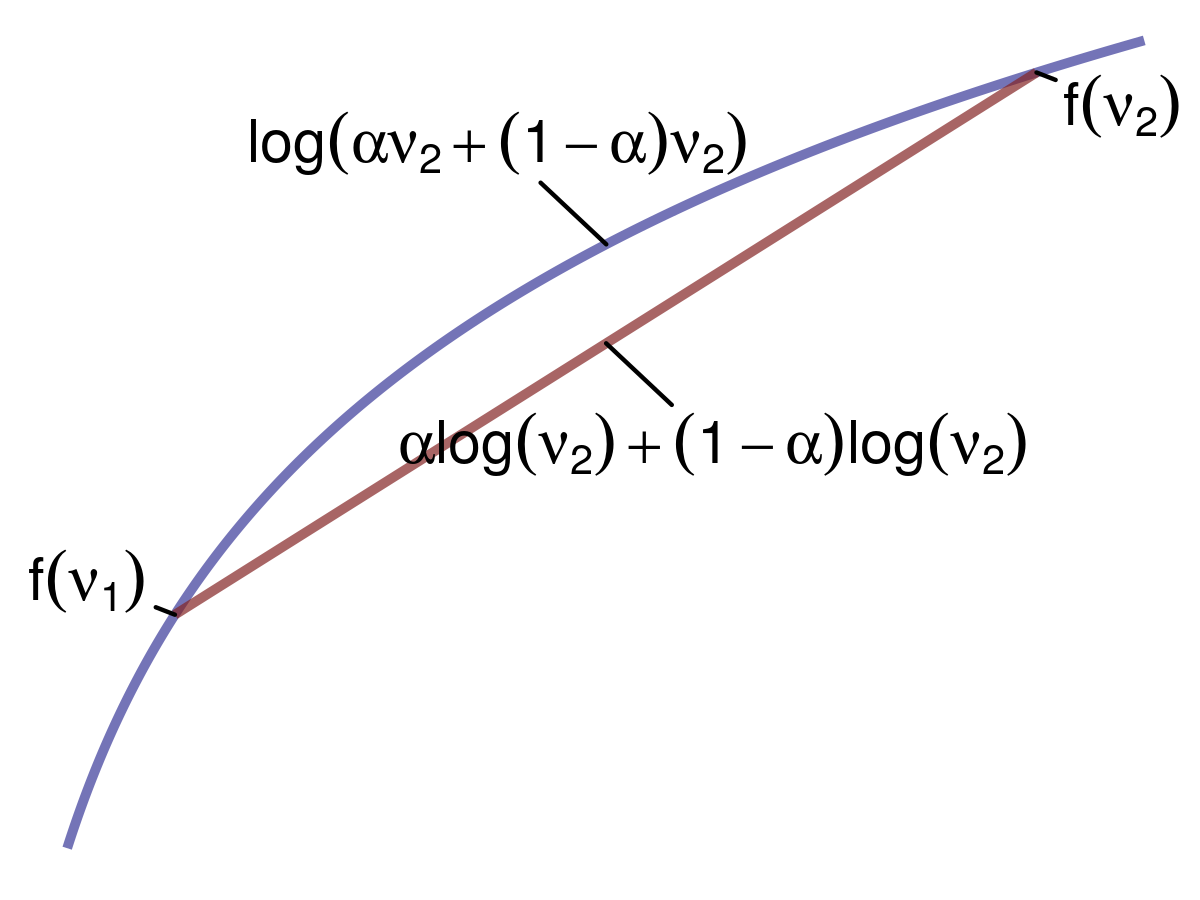
\includegraphics{figs/tm/jensen.png}
\caption{}
\end{figure}

We can apply this inequality to concave functions. If we have two points
(say \(v_1\) and \(v_2\)), and we average the function \(f\) that is
\emph{concave} at those two points; it will be less than the function
\(f\) applied to the average of those two points -- that is,
\(f(\mathbb{E}[X]) \geq \mathbb{E}[f(X)]\). Let's assume that
\(f(v)=\log{v}\). The weighted average between two points would
therefore be \(\log{[\alpha v_1 + (1-\alpha)v_2]}\), and the average of
the function at those two points would be
\(\alpha \log{v_1} + (1-\alpha)\log{v_2}\). This gives us the following
inequality:
\(\log{[\alpha v_1 + (1-\alpha)v_2]} \ge \alpha \log{v_1} + (1-\alpha)\log{v_2}\).

We're going to exploit the use of this inequality to calculate the
evidence lower bound (ELBO) for our variational inference procedure.
Given the log probability of our data \(\log{p(x)}\), let's also
consider all possible latent variables \(z\). To do this, we'll
marginalize out \(z\):

\[
\log{p(x)} = \log{\int_z p(x,z)}
\]

To introduce our distribution \(q\), we'll multiply by 1:

\[
\begin{aligned}
\log{p(x)} &= \log{\int_z p(x,z) \frac{q(z)}{q(z)}}\\
            &= \log{\int_z \frac{p(x,z)}{q(z)} q(z)}\\
            &= \log{\mathbb{E}_q [\frac{p(x,z)}{q(z)}]}
\end{aligned}
\]

Now we can apply Jensen's Inequality. We just derived the function
applied to the expectation, which was the left term of the inequality.
Now, the right term is the expectation of function, giving us:

\[
\begin{aligned}
\log{p(x)} = \log{\mathbb{E}_q [\frac{p(x,z)}{q(z)}]}
&\ge \mathbb{E}_q [\log{\frac{p(x,z)}{q(z)}}]\\
                                        &= \mathbb{E}_q [\log p(x,z)] - \mathbb{E}_q [\log q(z)]
\end{aligned}
\]

Turning the log of a quotient into a difference has a useful side
effect: \(\mathbb{E}_q [\log q(z)]\) is simply the entropy of the
variational distribution \(q\). We cannot optimize this part of the
equation; however, we \emph{can} maximize
\(\mathbb{E}_q [\log p(x,z)]\). By doing so, we will drive the equation
closer and closer to \(\log {p(x)}\), and ideally as far as the entropy
term will allow. This term we aim to maximize is the ELBO, and it will
give us a tight lower bound of \(\log{p(x)}\).

\subsubsection{ELBO and KL Divergence}\label{elbo-and-kl-divergence}

Maximizing the ELBO is equivalent to minimizing the KL divergence. To
see this, let's rewrite out joint probability distribution of our data
\(x\) and latent parameters \(z\) as

\[
p(z|x) = \frac{p(x,x)}{p(x)}\\
\]

Now, let's take the KL divergence between this distribution and the
variational distribution \(q\):

\[
\begin{aligned}
\text{KL}(q(z) || p(z|x)) &= \mathbb{E}_q [\log{\frac{q(z)}{p(z|x)}}]\\
                        &= \mathbb{E}_q [\log{q(z)} - \log{q(z)}]\\
                        &= \mathbb{E}_q [\log{q(z)}] - \mathbb{E}_q [\log{p(z|x)}]\\
                        &= \mathbb{E}_q [\log{q(z)}] - \mathbb{E}_q [\log{\frac{p(x,z)}{p(x)}}]\\
                        &= \mathbb{E}_q [\log{q(z)}] - \mathbb{E}_q [\log{p(x,z)} - \log{p(x)}]\\
                        &= \mathbb{E}_q [\log{q(z)}] - \mathbb{E}_q [\log{p(x,z)}] + \log{p(x)}
\end{aligned}
\]

When we optimize, the log probability of our data \(\log{p(x)}\) will
vanish because it's a constant, so we can rewrite this as

\[
\begin{aligned}
\text{KL}(q(z) || p(z|x)) &= \mathbb{E}_q [\log{q(z)}] - \mathbb{E}_q [\log{p(x,z)}]\\
                        &= -(\mathbb{E}_q [\log{p(x,z)}] - \mathbb{E}_q [\log{q(z)}])
\end{aligned}
\]

Thus, minimizing the KL divergence is the same as maximizing the ELBO.

\subsubsection{Mean Field Method}\label{mean-field-method}

One way of writing our variational distribution is via the mean field
method where we fully factorize our latent variables such that we assume
that they are completely independent of one another. For our variational
distribution \(q\) over latent parameters \(z\) we have

\[
q(z_1,\dots,z_N) = \prod_{i=1}^N q(z_i)
\]

It should be obvious that, given this assumption, \(p \neq q\) because
in \(p\), the latent variables are dependent upon one another. This mean
field method is a good starting point for deriving a variational
distribution, but sometimes it doesn't work, so other strategies to
forming the variational distribution would be required.

\subsection{LDA}\label{lda}

LDA follows the following generative process:

\begin{figure}[htbp]
\centering
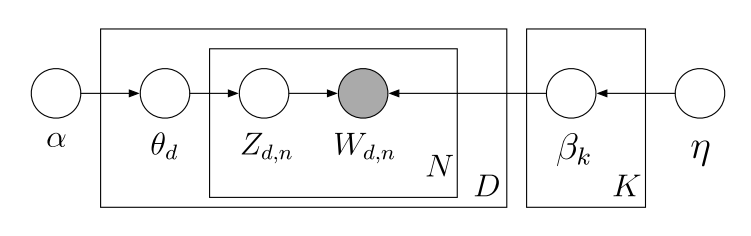
\includegraphics{figs/tm/lda_graphical_model.png}
\caption{}
\end{figure}

The joint distribution over all latent variables \(\theta\) and \(z\)
and observed data \(w\) is then

\[
p(\theta,z,w|\alpha,\beta) = \prod_d p(\theta_d|\alpha) \prod_n p(w_{d,n}|z_{d,n},\beta) p(z_{d,n}|\theta_d)
\]

where

\[
\begin{aligned}
&p(\theta_d|\alpha) = \frac{\Gamma (\sum_i \alpha_i)}{\prod_i \Gamma (\alpha_i)} \prod_i \theta_{d,k}^{\alpha_i -1} \text{, (Dirichlet)}\\
&p(z_{d,n}|\theta_d) = \prod_n \prod_i \theta_i^{1[z_n=i]} \text{, (Multinomial)}\\
&p(w_{d,n}|z_{d,n},\beta) = \prod_v \prod_i \beta_{i,v}^{1[w_{d,n}=v,z_{d,n}=i]} \text{, (Multinomial)}
\end{aligned}
\]

Now, our variational distribution for LDA will be a mean field
distribution where we assume complete independence between each
\(\theta\) and between all topic assignments \(z\), i.e., a fully
factored form:

\[
q(\theta,z|\gamma,\phi) = \prod_d q(\theta_d|\gamma_d) \prod_n q(z_{d,n}|\phi_{d,n})
\]

where \(\gamma \thicksim \text{Dirichlet}\) and
\(\phi \thicksim \text{Multinomial}\) are our variational parameters.
\(\theta_d\) will be a length \(K\) non-negative vector representing the
distribution over topics \(\gamma_d\) for document \(d\). Note that each
vector does \emph{not} sum to 1. \(z_{d,n}\) will also be a length \(K\)
vector, but instead is a distribution over topic assignments
\(\phi_{d,n}\) for each token \(z_{d,n}\). Each vector \text{does} sum
to 1.

Recall that the ELBO is
\(\mathbb{E}_q [\log p(x,z)] - \mathbb{E}_q [\log q(z)]\), where \(x\)
is our observed data and \(z\) are our latent variables. In LDA, \(w\)
is our observed data, and \(\theta\) and \(z\) are our latent variables.
Using the joint distribution over latent variables shown above, we have

\[
\begin{aligned}
\log p&(w|\alpha,\beta) \geq L(\gamma,\phi|\alpha,\beta) \\
    &= \mathbb{E}_q [\log  p(\theta,z,w|\alpha,\beta)] - \mathbb{E}_q [\log q(\theta,z)] \\
    &= \mathbb{E}_q [\log p(\theta|\alpha)p(z|\theta)p(w|z,\beta)] - \mathbb{E}_q [\log q(\theta)q(z)]\\
    &= \mathbb{E}_q [\log p(\theta|\alpha) + \log p(z|\theta) + \log p(w|z,\beta)] - \mathbb{E}_q [\log q(\theta) + \log q(z)]\\
    &= \mathbb{E}_q [\log p(\theta|\alpha)] + \mathbb{E}_q [\log p(z|\theta)] + \mathbb{E}_q [\log p(w|z,\beta)] - \mathbb{E}_q [\log q(\theta)] - \mathbb{E}_q[\log q(z)]\\
    &= \mathbb{E}_q [\log p(\theta|\alpha)] + \mathbb{E}_q [\log p(z|\theta)] + \mathbb{E}_q [\log p(w|z,\beta)] + \mathbb{H}_q [\gamma] + \mathbb{H}_q[\phi]
\end{aligned} 
\]

Before we continue, note that \(\mathbb{E}_q\) means the expectation
with respect to all parameters in our variational distribution \(q\), so
\(\theta\) and \(z\).

\subsubsection{\texorpdfstring{Expectation of
p(\(\theta|\alpha)\)}{Expectation of p(\textbackslash{}theta\textbar{}\textbackslash{}alpha)}}\label{expectation-of-pthetaalpha}

To calculate \(\mathbb{E}[\log p(\theta | \alpha)]\), where \(\theta\)
is our variational parameter, let's first recall that it is a Dirichlet
distribution; therefore, we have

\[
\begin{aligned}
\mathbb{E}_q [\log p(\theta | \alpha)] &= \mathbb{E}_q \log{[\frac{\Gamma (\sum_i \alpha_i)}{\prod_i \Gamma (\alpha_i)} \prod_i \theta_{d,k}^{\alpha_i -1}]}\\
        &=  \mathbb{E}_q \log \Gamma (\sum_i^k \alpha_i) - \mathbb{E}_q \sum_i^k \log \Gamma (\alpha_i) + \mathbb{E}_q \sum_i^k (\alpha_i -1) \log \theta \\
        &= \log \Gamma (\sum_i^k \alpha_i) - \sum_i^k \log \Gamma (\alpha_i) + \sum_i^k (\alpha_i -1) \mathbb{E}_q \log \theta \\
\end{aligned}
\]

Note that \(\mathbb{E}_q [f(\alpha)] = f(\alpha)\) because \(\alpha\) is
not one of the latent parameters in our variational distribution \(q\).
Now we have to calculate \(\mathbb{E}_q \log \theta\) where
\(\theta \thicksim \text{Dirichlet}\). We must first convert this
Dirichlet to its exponential form (given the fact that it belongs to the
exponential family). First, we exponentiate the log of
\(p(\theta | \alpha)\):

\[
\exp{[\log \Gamma (\sum_i^k \alpha_i) - \sum_i^k \log \Gamma (\alpha_i) + (\sum_i^k (\alpha_i -1) \log \theta)]}
\]

A pdf belonging to the exponential family has the form

\[
p(x|\theta) = h(x) \exp{[\theta^T \phi (x) - A(\theta)]}
\]

where \(\theta\) are the natural or canonical parameters, \(\phi (x)\)
is a vector of sufficient statistics, \(h (x)\) is a scaling constant
that is often equal to 1, and \(A (\theta)\) is the log partition
function. If we make one slight adjustment to the Dirichlet in
exponential family form, we can these components more easily:

\[
\exp{[(\sum_i^k (\alpha_i -1) \log \theta) - (\sum_i^k \log \Gamma (\alpha_i) + \log \Gamma (\sum_i^k \alpha_i))]}
\]

where \(\sum_i^k (\alpha_i -1)\) are the natural parameters,
\(\log \theta\) is the vector of sufficient statistics, and
\(\sum_i^k \log \Gamma (\alpha_i) + \log \Gamma (\sum_i^k \alpha_i)\) is
the log partition function. Taking the derivative of the log partition
function with respect to the natural parameters results in the
expectation of the sufficient statistic. Recall that we are working with
\(q(\theta_d|\gamma_d)\) there, our variational distribution, and not
\(p(\theta_d|\alpha)\):

\[
\begin{aligned}
\mathbb{E}_q[\log \theta] &= \frac{\partial}{\partial \gamma_i} (\log \Gamma (\gamma_i) + \log \Gamma (\sum_j^k \gamma_j)) \\
                                    &= \Psi (\gamma_i) - \Psi (\sum_j^k \gamma_j)
\end{aligned}
\]

And so we have

\[
\begin{aligned}
\mathbb{E}_q [\log p(\theta | \alpha)] &= \log \Gamma (\sum_i^k \alpha_i) - \sum_i^k \log \Gamma (\alpha_i) + \sum_i^k (\alpha_i -1) (\Psi (\gamma_i) - \Psi (\sum_j^k \gamma_j)) \\
\end{aligned}
\]

\subsubsection{\texorpdfstring{Expectation of
p(\(z|\theta)\)}{Expectation of p(z\textbar{}\textbackslash{}theta)}}\label{expectation-of-pztheta}

For this expectation, we do the following:

\[
\begin{aligned}
\mathbb{E}_q [\log p(z|\theta)] &= \mathbb{E}_q \log [\prod_n \prod_i \theta_i^{1[z_n=i]}]\\
                    &= \mathbb{E}_q [\sum_n \sum_i \log \theta_i^{1[z_n=i]}]\\
                    &= \sum_n \sum_i \mathbb{E}_q [\log \theta_i^{1[z_n=i]}]\\
                    &= \sum_n \sum_i \mathbb{E}_q [1[z_n=i] \log \theta_i]
\end{aligned}
\]

Recall that \(1[z_n=i]\) is an indicator of whether a particular word's
topic assignment \(z_n\) is equal to topic \(i\). If so, then we add the
probability \(\theta_{d,i}\) of this topic in document \(d\) to the
summation. Because in our variational distribution \(q\) we assume that
\(\theta\) and \(z\) are independent, we can do the following:

\[
\begin{aligned}
\mathbb{E}_q [\log p(z|\theta)] &= \sum_n \sum_i \mathbb{E}_q [1[z_n=i] \log \theta_i]\\
                    &= \sum_n \sum_i \mathbb{E}_q 1[z_n=i] \mathbb{E}_q \log \theta_i\\
\end{aligned}
\]

The expectation of this indicator function is just a measure of how much
a particular token \(n\) takes on a topic assignment \(i\), which we'll
call \(\phi_{n,i}\):

\[
\begin{aligned}
\mathbb{E}_q [\log p(z|\theta)] &= \sum_n \sum_i \phi_{n,i} \mathbb{E}_q \log \theta_i\\
                    &= \sum_n \sum_i \phi_{n,i} (\Psi (\gamma_i) - \Psi (\sum_j^k \gamma_j))
\end{aligned}
\]

\subsubsection{\texorpdfstring{Expectation of
p(\(w|z,\beta)\)}{Expectation of p(w\textbar{}z,\textbackslash{}beta)}}\label{expectation-of-pwzbeta}

Here we are simply looking up the probability \(\beta\) of a topic
assignment \(z_{d,n}\) for the word \(w_{d,n}\).

\[
\begin{aligned}
\mathbb{E}_q [\log p(w|z,\beta)] &= \mathbb{E}_q [\log \prod_v \prod_i \beta_{i,v}^{1[w_{d,n}=v,z_{d,n}=i]}] \\
                                &= \mathbb{E}_q [\sum_v \sum_i \log \beta_{i,v}^{1[w_{d,n}=v,z_{d,n}=i]}] \\
                                &= \sum_v \sum_i \mathbb{E}_q [\log \beta_{i,v}^{1[w_{d,n}=v,z_{d,n}=i]}] \\
                                &= \sum_v \sum_i \mathbb{E}_q [1[w_{d,n}=v,z_{d,n}=i] \log \beta_{i,v}] \\
                                &= \sum_v \sum_i \mathbb{E}_q [1[w_{d,n}=v,z_{d,n}=i]] \log \beta_{i,v} \\
                                &= \sum_v \sum_i \mathbb{E}_q [1[w_{d,n}=v]1[z_{d,n}=i]] \log \beta_{i,v} \\
                                &= \sum_v \sum_i 1[w_{d,n}=v] \mathbb{E}_q [1[z_{d,n}=i]] \log \beta_{i,v} \\
\end{aligned}
\]

Recall that we already defined \(\mathbb{E}_q 1[z_n=i] = \phi_{n,i}\),
leaving us with

\[
\begin{aligned}
\mathbb{E}_q [\log p(w|z,\beta)] &= \sum_v \sum_i 1[w_{d,n}=v] \phi_{n,i} \log \beta_{i,v}
\end{aligned}
\]

\subsubsection{\texorpdfstring{Entropy of \(\gamma\) and
\(\phi\)}{Entropy of \textbackslash{}gamma and \textbackslash{}phi}}\label{entropy-of-gamma-and-phi}

We can simply look up the entropy of a Dirichlet for \(\gamma\) and the
entropy of a multinomial for \(\phi_{d,n}\), giving us

\[
\begin{aligned}
\mathbb{H}_q [\gamma] &= -\log \Gamma (\sum_j \gamma_j) + \sum_i \log \Gamma(\gamma_i) - \sum_i (\gamma_i -1) (\Psi (\gamma_i) - \Psi (\sum_j^k \gamma_j))\\
\mathbb{H}_q [\phi_{d,n}] &= -\sum_i \phi_{d,n,i} \log \phi_{d,n,i}
\end{aligned}
\]

\subsubsection{Complete Objective
Function}\label{complete-objective-function}

Now that we calculated the expectations and entropies we need, we can
fill in our original equation:

\[
\begin{aligned}
\mathbb{E}_q &[\log  p(\theta,z,w|\alpha,\beta)] - \mathbb{E}_q [\log q(\theta,z)] \\
    &= \mathbb{E}_q [\log p(\theta|\alpha)] + \mathbb{E}_q [\log p(z|\theta)] + \mathbb{E}_q [\log p(w|z,\beta)] + \mathbb{H}_q [\gamma] + \mathbb{H}_q[\phi_{d,n}] \\
\end{aligned} 
\]

Giving us

\[
\begin{aligned}
    \mathbb{E}_q &[\log  p(\theta,z,w|\alpha,\beta)] - \mathbb{E}_q [\log q(\theta,z)] = \\
                &\log \Gamma (\sum_i \alpha_j) - \sum_i \log \Gamma (\alpha_i) + \sum_i^k (\alpha_i -1) (\Psi (\gamma_i) - \Psi (\sum_j^k \gamma_j)) \\
                &+ \sum_n \sum_i \phi_{n,i} (\Psi (\gamma_i) - \Psi (\sum_j^k \gamma_j)) \\
                &+ \sum_n \sum_i \sum_v 1[w_n=v] \phi_{n,i} \log \beta_{i,v} \\
                &- \log \Gamma (\sum_j \gamma_j) + \sum_i \log \Gamma(\gamma_i) - \sum_i (\gamma_i -1) (\Psi (\gamma_i) - \Psi (\sum_j^k \gamma_j)) \\
                &- \sum_n \sum_i \phi_{n,i} \log \phi_{n,i}
\end{aligned} 
\]

\subsubsection{Parameter Optimization}\label{parameter-optimization}

To derive our parameter updates for variational EM, we need to maximize
the objective function above with respect to our target parameter.

\paragraph{\texorpdfstring{Optimization for
\(\phi\)}{Optimization for \textbackslash{}phi}}\label{optimization-for-phi}

Using the objective function above, we'll isolate every term that is a
function of \(phi\), and using the constraint \(\sum_i \phi_{n,i}=1\),
we'll perform the following optimization:

\[
\begin{aligned}
\frac{\partial L}{\partial \phi_{n,i}} &= \frac{\partial}{\partial \phi_{n,i}}[\phi_{n,i} (\Psi(\gamma_i) - \Psi(\sum_j \gamma_j)) + \sum_j 1[w_n = v] \phi_{n,i} \log \beta_{i,v} \\ 
&\qquad- \phi_{n,i} \log \phi_{n,i} + \lambda_n (\phi_{n,i} - 1)]\\
    &=\Psi ' (\gamma) - \Psi ' (\sum_j \gamma_j) + 1[w_n = v] \log \beta_{i,v} - \log \phi_{n,i} - 1 + \lambda
\end{aligned}
\]

Then, setting to this to zero, we get

\[
\begin{aligned}
  0 &=\Psi ' (\gamma) - \Psi ' (\sum_j \gamma_j) + 1[w_n = v] \log \beta_{i,v} - \log \phi_{n,i} - 1 + \lambda\\
  \log \phi_{n,i} &= \Psi ' (\gamma) - \Psi ' (\sum_j \gamma_j) + 1[w_n = v] \log \beta_{i,v} - 1 + \lambda \\
  \phi_{n,i} &= \exp [\Psi ' (\gamma) - \Psi ' (\sum_j \gamma_j) + 1[w_n = v] \log \beta_{i,v} - 1 + \lambda]\\
      &= \beta_{i,v}^{1[w_n = v]} \exp [\Psi ' (\gamma) - \Psi ' (\sum_j \gamma_j)] \exp [- 1 + \lambda]\\
      &= c_{n,i} \beta_{i,v}^{1[w_n = v]} \exp [\Psi ' (\gamma) - \Psi ' (\sum_j \gamma_j)]
\end{aligned}
\]

where \(c_{n,i}=\exp [\lambda - 1]\). Because we don't know \(\lambda\),
we will simply calculate the unnormalized \(\phi_{n,i}\) and then
normalize to enforce the constraint that \(\sum_i \phi_{n,i}=1\).
Therefore, we have

\[
\begin{aligned}
\phi_{n,i} &\propto \beta_{i,v}^{1[w_n = v]} \exp [\Psi ' (\gamma) - \Psi ' (\sum_j \gamma_j)]
\end{aligned}
\]

\paragraph{\texorpdfstring{Optimization for
\(\gamma_i\)}{Optimization for \textbackslash{}gamma\_i}}\label{optimization-for-gammaux5fi}

Now we'll take all terms that are a function of \(\gamma_i\):

\[
\begin{aligned}
\frac{\partial L}{\partial \gamma_i} &= \frac{\partial}{\partial \gamma_i}[(\alpha_i -1) (\Psi (\gamma_i) - \Psi (\sum_j \gamma_j)) \\
                &\qquad + \sum_n \phi_{n,i} (\Psi (\gamma_i) - \Psi (\sum_j \gamma_j)) \\
                &\qquad - \log \Gamma (\sum_j \gamma_j) + \log \Gamma(\gamma_i) \\
                &\qquad - (\gamma_i -1) (\Psi (\gamma_i) - \Psi (\sum_j \gamma_j))] \\
                &= \frac{\partial}{\partial \gamma_i} [\alpha_i \Psi (\gamma_i) - \alpha_i \Psi (\sum_j \gamma_j) - \Psi (\gamma_i) + \Psi (\sum_j \gamma_j)\\
                &\qquad + \sum_n \phi_{n,i} \Psi (\gamma_i) - \sum_n \phi_{n,i} \Psi (\sum_j \gamma_j)\\
                &\qquad - \log \Gamma (\sum_j \gamma_j) + \log \Gamma (\gamma_i) \\
                &\qquad - \gamma_i \Psi (\gamma_i) + \gamma_i \Psi (\sum_j \gamma_j) + \Psi (\gamma_i) - \Psi(\sum_j \gamma_j)]\\
                &= \alpha_i \Psi' (\gamma_i) - \alpha_i \Psi' (\sum_j \gamma_j) - \Psi' (\gamma_i) + \Psi' (\sum_j \gamma_j)\\
                &\qquad + \sum_n \phi_{n,i} \Psi' (\gamma_i) - \sum_n \phi_{n,i} \Psi' (\sum_j \gamma_j)\\
                &\qquad - \Psi (\sum_j \gamma_j) + \Psi (\gamma_i) \\
                &\qquad - \gamma_i \Psi' (\gamma_i) - \Psi (\gamma_i) + \gamma_i \Psi' (\sum_j \gamma_j) + \Psi (\sum_j \gamma_j) + \Psi' (\gamma_i) - \Psi' (\sum_j \gamma_j)\\
                &= \alpha_i \Psi' (\gamma_i) - \alpha_i \Psi' (\sum_j \gamma_j) - \Psi' (\gamma_i) + \Psi' (\sum_j \gamma_j)\\
                &\qquad + \sum_n \phi_{n,i} \Psi' (\gamma_i) - \sum_n \phi_{n,i} \Psi' (\sum_j \gamma_j)\\
                &\qquad - \gamma_i \Psi' (\gamma_i) + \gamma_i \Psi' (\sum_j \gamma_j) + \Psi' (\gamma_i) - \Psi' (\sum_j \gamma_j)
\end{aligned}
\]

Now combine terms:

\[
\begin{aligned}
\Psi' (\gamma_i)(\alpha_i - 1 + \sum_n \phi_{n,i} - \gamma_i + 1) &= \Psi' (\sum_j \gamma_j)(\alpha_i + \sum_n \phi_{n,i} - \gamma_j)\\
\Psi' (\gamma_i)(\alpha_i + \sum_n \phi_{n,i} - \gamma_i) &= \Psi' (\sum_j \gamma_j)(\alpha_i + \sum_n \phi_{n,i} - \gamma_j)\\
\end{aligned}
\]

Then set this to zero:

\[
\begin{aligned}
0 &= \Psi' (\gamma_i)(\alpha_i + \sum_n \phi_{n,i} - \gamma_i) - \Psi' (\sum_j \gamma_j)(\alpha_i + \sum_n \phi_{n,i} - \gamma_j)\\
\end{aligned}
\]

Leaving us with

\[
\begin{aligned}
\gamma_i &= \alpha_i + \sum_n \phi_{n,i}
\end{aligned}
\]

\paragraph{\texorpdfstring{Optimization for
\(\beta\)}{Optimization for \textbackslash{}beta}}\label{optimization-for-beta}

Now, we'll extract all terms that are a function of \(\beta\) and add
the constrain \(\sum_v \beta_{i,v} = 1\):

\[
\begin{aligned}
\frac{\partial L}{\partial \beta} &= \frac{\partial}{\partial \beta}[\sum_n \sum_i \sum_v 1[w_n=v]\phi_{n,i} \log \beta_{i,v} + \sum_i \lambda_i (\sum_v \beta_{i,v} - 1)]\\
                &=\sum_n \sum_i \sum_v \frac{1[w_n=v]\phi_{n,i}}{\beta_{i,v}} + \sum_i \lambda_i\\
\end{aligned}
\]

Setting this to 0 results in

\[
\begin{aligned}
0 &=\sum_n \sum_i \sum_v \frac{1[w_n=v]\phi_{n,i}}{\beta_{i,v}} + \sum_i \lambda_i\\
- \beta_{i,v} \sum_i \lambda_i &=\sum_n \sum_i \sum_v 1[w_n=v]\phi_{n,i}\\
\beta_{i,v} &= c_{i,v} \sum_n \sum_i \sum_v 1[w_n=v]\phi_{n,i}^{(k)}
\end{aligned}
\]

where \(c_{i,v} = -\frac{1}{\sum_i \lambda_i}\). Like what we did for
\(\phi\), we will calculate unnormalized \(\beta\) and then normalize to
satisfy the constraint. Our final update is the following:

\[
\begin{aligned}
\beta_{i,v} &\propto \sum_n \sum_i \sum_v 1[w_n=v]\phi_{n,i}
\end{aligned}
\]

\begin{Shaded}
\begin{Highlighting}[]
\KeywordTok{library}\NormalTok{(tidyverse)}

\NormalTok{vocab <-}\StringTok{ }\KeywordTok{c}\NormalTok{(}\StringTok{"river"}\NormalTok{,}\StringTok{"stream"}\NormalTok{,}\StringTok{"bank"}\NormalTok{,}\StringTok{"money"}\NormalTok{,}\StringTok{"loan"}\NormalTok{)}
\NormalTok{topic1 <-}\StringTok{ }\KeywordTok{c}\NormalTok{(.}\DecValTok{333}\NormalTok{,.}\DecValTok{333}\NormalTok{,.}\DecValTok{333}\NormalTok{,}\DecValTok{0}\NormalTok{,}\DecValTok{0}\NormalTok{)}
\NormalTok{topic2 <-}\StringTok{ }\KeywordTok{c}\NormalTok{(}\DecValTok{0}\NormalTok{,}\DecValTok{0}\NormalTok{,.}\DecValTok{333}\NormalTok{,.}\DecValTok{333}\NormalTok{,.}\DecValTok{333}\NormalTok{)}
\NormalTok{topics <-}\StringTok{ }\NormalTok{topic1 +}\StringTok{ }\NormalTok{topic2}
\NormalTok{K <-}\StringTok{ }\DecValTok{2}
\NormalTok{V <-}\StringTok{ }\KeywordTok{length}\NormalTok{(vocab)}
\NormalTok{N <-}\StringTok{ }\DecValTok{16}
\NormalTok{corpus <-}\StringTok{   }\KeywordTok{rbind}\NormalTok{(}\KeywordTok{matrix}\NormalTok{(}\KeywordTok{rep}\NormalTok{(}\KeywordTok{sample}\NormalTok{(vocab,N,topic1,}\DataTypeTok{replace=}\NormalTok{T),}\DecValTok{7}\NormalTok{),}\DecValTok{7}\NormalTok{,N),}
                 \KeywordTok{matrix}\NormalTok{(}\KeywordTok{rep}\NormalTok{(}\KeywordTok{sample}\NormalTok{(vocab,N,topics,}\DataTypeTok{replace=}\NormalTok{T),}\DecValTok{10}\NormalTok{),}\DecValTok{10}\NormalTok{,N),}
                 \KeywordTok{matrix}\NormalTok{(}\KeywordTok{rep}\NormalTok{(}\KeywordTok{sample}\NormalTok{(vocab,N,topic2,}\DataTypeTok{replace=}\NormalTok{T),}\DecValTok{5}\NormalTok{),}\DecValTok{5}\NormalTok{,N))}
\NormalTok{M <-}\StringTok{ }\KeywordTok{nrow}\NormalTok{(corpus)}

\NormalTok{start <-}\StringTok{ }\KeywordTok{t}\NormalTok{(}\KeywordTok{apply}\NormalTok{(corpus, }\DecValTok{1}\NormalTok{, function(x) }\KeywordTok{c}\NormalTok{(}\KeywordTok{sum}\NormalTok{(x==vocab[}\DecValTok{1}\NormalTok{]),}\KeywordTok{sum}\NormalTok{(x==vocab[}\DecValTok{2}\NormalTok{]),}\KeywordTok{sum}\NormalTok{(x==vocab[}\DecValTok{3}\NormalTok{]),}\KeywordTok{sum}\NormalTok{(x==vocab[}\DecValTok{4}\NormalTok{]),}\KeywordTok{sum}\NormalTok{(x==vocab[}\DecValTok{5}\NormalTok{]))))}
\NormalTok{docnames <-}\StringTok{ }\KeywordTok{paste}\NormalTok{(}\StringTok{"D"}\NormalTok{,}\DecValTok{1}\NormalTok{:M,}\DataTypeTok{sep=}\StringTok{""}\NormalTok{)}
\KeywordTok{rownames}\NormalTok{(start) <-}\StringTok{ }\NormalTok{docnames}
\KeywordTok{colnames}\NormalTok{(start) <-}\StringTok{ }\NormalTok{vocab}

\NormalTok{topicassign <-}\StringTok{ }\KeywordTok{matrix}\NormalTok{(}\KeywordTok{sample}\NormalTok{(}\KeywordTok{c}\NormalTok{(}\DecValTok{0}\NormalTok{,}\DecValTok{1}\NormalTok{),M*N,}\DataTypeTok{replace=}\NormalTok{T),M,N,}\DataTypeTok{byrow=}\NormalTok{T)}

\NormalTok{df <-}\StringTok{ }\OtherTok{NULL}
\NormalTok{for(i in }\DecValTok{1}\NormalTok{:M)\{}
  \NormalTok{df <-}\StringTok{ }\KeywordTok{rbind}\NormalTok{(df,}\KeywordTok{cbind}\NormalTok{(corpus[i,],}\KeywordTok{rep}\NormalTok{(docnames[i]),topicassign[i,]))}
\NormalTok{\}}
\NormalTok{df <-}\StringTok{ }\KeywordTok{data.frame}\NormalTok{(df)}
\KeywordTok{names}\NormalTok{(df) <-}\StringTok{ }\KeywordTok{c}\NormalTok{(}\StringTok{'word'}\NormalTok{,}\StringTok{'doc'}\NormalTok{,}\StringTok{'topic'}\NormalTok{)}
\NormalTok{df_original <-}\StringTok{ }\NormalTok{df}

\NormalTok{nu <-}\StringTok{ }\NormalTok{.}\DecValTok{25}
\NormalTok{alpha <-}\StringTok{ }\NormalTok{.}\DecValTok{5}

\NormalTok{for (iter in }\DecValTok{1}\NormalTok{:}\DecValTok{100}\NormalTok{)\{}
  
  \KeywordTok{cat}\NormalTok{(}\StringTok{"i="}\NormalTok{,iter,}\StringTok{"}\CharTok{\textbackslash{}n}\StringTok{"}\NormalTok{,}\DataTypeTok{sep=}\StringTok{""}\NormalTok{)}
  \KeywordTok{print}\NormalTok{(}\KeywordTok{xtabs}\NormalTok{(~}\StringTok{ }\NormalTok{word+topic,df))}
  \KeywordTok{cat}\NormalTok{(}\StringTok{"}\CharTok{\textbackslash{}n}\StringTok{"}\NormalTok{,}\DataTypeTok{sep=}\StringTok{""}\NormalTok{)}
  
  \NormalTok{for (i in }\DecValTok{1}\NormalTok{:}\KeywordTok{nrow}\NormalTok{(df))\{}
    
    \NormalTok{w <-}\StringTok{ }\KeywordTok{as.vector}\NormalTok{(df[i,}\DecValTok{1}\NormalTok{])}
    \NormalTok{d <-}\StringTok{ }\KeywordTok{as.vector}\NormalTok{(df[i,}\DecValTok{2}\NormalTok{])}
    
    \NormalTok{civk <-}\StringTok{ }\NormalTok{df[-i,] %>%}
\StringTok{      }\KeywordTok{group_by}\NormalTok{(word,doc,topic) %>%}
\StringTok{      }\KeywordTok{summarise}\NormalTok{(}\DataTypeTok{civk=}\KeywordTok{n}\NormalTok{())}
    \NormalTok{cik <-}\StringTok{ }\NormalTok{df[-i,] %>%}
\StringTok{      }\KeywordTok{group_by}\NormalTok{(doc,topic) %>%}
\StringTok{      }\KeywordTok{summarise}\NormalTok{(}\DataTypeTok{cik=}\KeywordTok{n}\NormalTok{())}
    \NormalTok{cvk <-}\StringTok{ }\NormalTok{df[-i,] %>%}
\StringTok{      }\KeywordTok{group_by}\NormalTok{(word,topic) %>%}
\StringTok{      }\KeywordTok{summarise}\NormalTok{(}\DataTypeTok{cvk=}\KeywordTok{n}\NormalTok{())}
    \NormalTok{niv <-}\StringTok{ }\NormalTok{df[-i,] %>%}
\StringTok{      }\KeywordTok{group_by}\NormalTok{(word,doc) %>%}
\StringTok{      }\KeywordTok{summarise}\NormalTok{(}\DataTypeTok{niv=}\KeywordTok{n}\NormalTok{())}
    \NormalTok{ck <-}\StringTok{ }\NormalTok{df[-i,] %>%}
\StringTok{      }\KeywordTok{group_by}\NormalTok{(topic) %>%}
\StringTok{      }\KeywordTok{summarise}\NormalTok{(}\DataTypeTok{words=}\KeywordTok{n}\NormalTok{())}
    \NormalTok{Li <-}\StringTok{ }\NormalTok{df[-i,] %>%}
\StringTok{      }\KeywordTok{group_by}\NormalTok{(doc) %>%}
\StringTok{      }\KeywordTok{summarise}\NormalTok{(}\DataTypeTok{words=}\KeywordTok{n}\NormalTok{())}
    
    \NormalTok{a <-}\StringTok{ }\KeywordTok{unlist}\NormalTok{((cvk[cvk$word==w,}\DecValTok{3}\NormalTok{] +}\StringTok{ }\NormalTok{nu))/}\KeywordTok{unlist}\NormalTok{((ck[,}\DecValTok{2}\NormalTok{] +}\StringTok{ }\NormalTok{V*nu))}
    \NormalTok{b <-}\StringTok{ }\KeywordTok{unlist}\NormalTok{((cik[cik$doc==d,}\DecValTok{3}\NormalTok{] +}\StringTok{ }\NormalTok{alpha))/}\KeywordTok{unlist}\NormalTok{((Li[Li$doc==d,}\DecValTok{2}\NormalTok{] +}\StringTok{ }\NormalTok{K*alpha))}
    \NormalTok{pqilk <-}\StringTok{ }\KeywordTok{unlist}\NormalTok{((a*b)/}\KeywordTok{sum}\NormalTok{(a*b))}
    \NormalTok{df[i,}\DecValTok{3}\NormalTok{] <-}\StringTok{ }\KeywordTok{sample}\NormalTok{(}\KeywordTok{c}\NormalTok{(}\DecValTok{0}\NormalTok{,}\DecValTok{1}\NormalTok{),}\DataTypeTok{size=}\DecValTok{1}\NormalTok{,}\DataTypeTok{prob=}\NormalTok{pqilk)}
  \NormalTok{\}}
\NormalTok{\}}

\NormalTok{est_alpha <-}\StringTok{ }\OtherTok{TRUE}
\NormalTok{alpha <-}\StringTok{ }\KeywordTok{rep}\NormalTok{(}\DecValTok{50}\NormalTok{/K,K)}
\NormalTok{beta <-}\StringTok{ }\KeywordTok{rdirichlet}\NormalTok{(K,}\KeywordTok{rep}\NormalTok{(}\DecValTok{1}\NormalTok{,V))}
\NormalTok{for (m_step in }\DecValTok{1}\NormalTok{:}\DecValTok{50}\NormalTok{)\{}
  
  \NormalTok{gamma <-}\StringTok{ }\KeywordTok{matrix}\NormalTok{(alpha +}\StringTok{ }\NormalTok{N/K,M,K,}\DataTypeTok{byrow=}\OtherTok{TRUE}\NormalTok{)}
  \NormalTok{phi <-}\StringTok{ }\KeywordTok{array}\NormalTok{(}\DecValTok{1}\NormalTok{/K,}\KeywordTok{c}\NormalTok{(M,N,K))}
  
  \NormalTok{## E step}
  \NormalTok{for (d in }\DecValTok{1}\NormalTok{:M)\{}
    \NormalTok{conv <-}\StringTok{ }\OtherTok{Inf}
    \NormalTok{tol <-}\StringTok{ }\FloatTok{1e-6}
    \NormalTok{while (tol <}\StringTok{ }\NormalTok{conv)\{}
      \NormalTok{phi0 <-}\StringTok{ }\NormalTok{phi}
      \NormalTok{gamma0 <-}\StringTok{ }\NormalTok{gamma}
      \NormalTok{for (n in }\DecValTok{1}\NormalTok{:N)\{}
        \NormalTok{for (i in }\DecValTok{1}\NormalTok{:K)\{}
          \NormalTok{phi[d,n,i] <-}\StringTok{ }\NormalTok{beta[i,corpus[d,n]==vocab] *}\StringTok{ }\KeywordTok{exp}\NormalTok{(}\KeywordTok{digamma}\NormalTok{(gamma[d,i]) -}\StringTok{ }\KeywordTok{digamma}\NormalTok{(}\KeywordTok{sum}\NormalTok{(gamma[d,])))}
        \NormalTok{\}}
        \NormalTok{phi[d,n,] <-}\StringTok{ }\NormalTok{phi[d,n,]/}\KeywordTok{sum}\NormalTok{(phi[d,n,])}
      \NormalTok{\}}
      \NormalTok{gamma[d,] <-}\StringTok{ }\NormalTok{alpha +}\StringTok{ }\KeywordTok{colSums}\NormalTok{(phi[d,,])}
      \NormalTok{conv <-}\StringTok{ }\KeywordTok{max}\NormalTok{(}\KeywordTok{c}\NormalTok{(}\KeywordTok{max}\NormalTok{(}\KeywordTok{abs}\NormalTok{(phi-phi0)),}\KeywordTok{max}\NormalTok{(}\KeywordTok{abs}\NormalTok{(gamma[d,]-gamma0[d,]))))}
    \NormalTok{\}}
  \NormalTok{\}}
  
  \NormalTok{## M step}
  \NormalTok{for (i in }\DecValTok{1}\NormalTok{:K)\{}
    \NormalTok{for (j in }\DecValTok{1}\NormalTok{:V)\{}
      \NormalTok{w_dnj <-}\StringTok{ }\NormalTok{corpus ==}\StringTok{ }\NormalTok{vocab[j]}
      \NormalTok{beta[i,j] <-}\StringTok{ }\KeywordTok{ifelse}\NormalTok{(}\KeywordTok{any}\NormalTok{(w_dnj),}\KeywordTok{sum}\NormalTok{(phi[,,i][w_dnj]),}\FloatTok{1e-20}\NormalTok{)}
    \NormalTok{\}}
    \NormalTok{beta[i,] <-}\StringTok{ }\NormalTok{beta[i,]/}\KeywordTok{sum}\NormalTok{(beta[i,])}
  \NormalTok{\}}
  
  \NormalTok{## alpha}
  \NormalTok{if (est_alpha ==}\StringTok{ }\OtherTok{TRUE}\NormalTok{)\{}
    \NormalTok{conv <-}\StringTok{ }\OtherTok{Inf}
    \NormalTok{tol <-}\StringTok{ }\FloatTok{1e-3}
    \NormalTok{iter <-}\StringTok{ }\DecValTok{1}
    \NormalTok{alpha_init <-}\StringTok{ }\DecValTok{100}
    \NormalTok{alpha <-}\StringTok{ }\NormalTok{alpha_init}
    \NormalTok{while (tol <}\StringTok{ }\NormalTok{conv |}\StringTok{ }\NormalTok{iter <}\StringTok{ }\DecValTok{100}\NormalTok{)\{}
      \NormalTok{if (}\KeywordTok{any}\NormalTok{(}\KeywordTok{is.na}\NormalTok{(alpha)))\{}
        \NormalTok{alpha_init <-}\StringTok{ }\NormalTok{alpha_init*}\DecValTok{10}
        \NormalTok{alpha <-}\StringTok{ }\NormalTok{alpha_init}
      \NormalTok{\}}
      \NormalTok{alpha0 <-}\StringTok{ }\NormalTok{alpha}
      \NormalTok{d1alpha <-}\StringTok{ }\NormalTok{M*(K*}\KeywordTok{digamma}\NormalTok{(K*alpha) -}\StringTok{ }\NormalTok{K*}\KeywordTok{digamma}\NormalTok{(alpha)) +}\StringTok{ }\KeywordTok{colSums}\NormalTok{(}\KeywordTok{digamma}\NormalTok{(gamma) -}\StringTok{ }\NormalTok{K*}\KeywordTok{digamma}\NormalTok{(}\KeywordTok{rowSums}\NormalTok{(gamma)))}
      \NormalTok{d2alpha <-}\StringTok{ }\NormalTok{M*(K *}\StringTok{ }\NormalTok{K *}\StringTok{ }\KeywordTok{trigamma}\NormalTok{(K*alpha) -}\StringTok{ }\NormalTok{K*}\KeywordTok{trigamma}\NormalTok{(alpha)) }\CommentTok{# note sure how to use the Kronecker-delta function here}
      \NormalTok{log_alpha <-}\StringTok{ }\KeywordTok{log}\NormalTok{(alpha) -}\StringTok{ }\NormalTok{d1alpha/(d2alpha*alpha +}\StringTok{ }\NormalTok{d1alpha) }
      \NormalTok{alpha <-}\StringTok{ }\KeywordTok{exp}\NormalTok{(log_alpha)}
      \NormalTok{conv <-}\StringTok{ }\KeywordTok{max}\NormalTok{(}\KeywordTok{abs}\NormalTok{(alpha-alpha0))}
      \NormalTok{iter <-}\StringTok{ }\NormalTok{iter +}\StringTok{ }\DecValTok{1}
    \NormalTok{\}}
  \NormalTok{\}}
  
  \CommentTok{# Check}
  \NormalTok{word_counter <-}\StringTok{ }\KeywordTok{matrix}\NormalTok{(}\DecValTok{0}\NormalTok{,V,K)}
  \NormalTok{for (d in }\DecValTok{1}\NormalTok{:M)\{}
    \NormalTok{for (n in }\DecValTok{1}\NormalTok{:N)\{}
      \NormalTok{word <-}\StringTok{ }\NormalTok{corpus[d,n] ==}\StringTok{ }\NormalTok{vocab}
      \NormalTok{topic <-}\StringTok{ }\KeywordTok{sample}\NormalTok{(}\KeywordTok{c}\NormalTok{(}\DecValTok{1}\NormalTok{,}\DecValTok{2}\NormalTok{),}\DecValTok{1}\NormalTok{,}\DataTypeTok{prob=}\NormalTok{beta[,word])}
      \NormalTok{word_counter[word,topic] <-}\StringTok{ }\NormalTok{word_counter[word,topic] +}\StringTok{ }\DecValTok{1}
    \NormalTok{\}}
  \NormalTok{\}}
  
  \KeywordTok{print}\NormalTok{(word_counter)}
\NormalTok{\}}
\end{Highlighting}
\end{Shaded}

\subsection{Supervised LDA}\label{supervised-lda}

For sLDA, we have the following generative model

\begin{figure}[htbp]
\centering
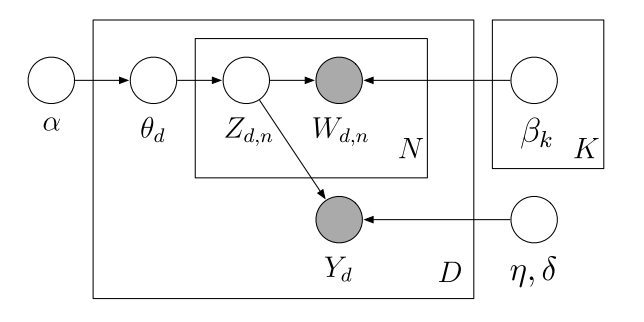
\includegraphics{figs/tm/slda_graphical_model.png}
\caption{}
\end{figure}

This has a similar joint distribution to LDA, but note \(\eta\),
\(\sigma^2\), and another observed variable \(y\). These are the
regression coefficients, model noise, and document labels, respectively:

\[
p(\theta,z,w,y|\eta,\alpha,\beta,\sigma^2) = \prod_d p(\theta_d|\alpha) p(y_d|z_{d,n},\eta,\sigma^2) \prod_n p(z_{d,n}|\theta_d)p(w_{d,n}|z_{d,n},\beta)
\]

where

\[
\begin{aligned}
&p(\theta_d|\alpha) = \frac{\Gamma (\sum_i \alpha_i)}{\prod_i \Gamma (\alpha_i)} \prod_i \theta_{d,k}^{\alpha_i -1} \text{, (Dirichlet)}\\
&p(z_{d,n}|\theta_d) = \prod_n \prod_i \theta_i^{1[z_n=i]} \text{, (Multinomial)}\\
&p(w_{d,n}|z_{d,n},\beta) = \prod_v \prod_i \beta_{i,v}^{1[w_{d,n}=v,z_{d,n}=i]} \text{, (Multinomial)}\\
&p(y_d|z_{d,n},\eta,\sigma^2) = \frac{1}{\sqrt{2 \pi \sigma^2}} \exp [-\frac{(y-\bar Z \eta)^2}{2\sigma^2}] \text{, (Normal)}
\end{aligned}
\]

where \(\bar Z\) is an \(K \times D\) matrix of topic proportions such
that \(\bar Z_{i,d}\) is the proportion topic \(i\) is represented out
of all topics for document \(d\). Note that \(\sum_i \bar Z_{i,d}=1\).

We'll again use the mean field method, giving us a fully factored form
of the latent variables \(\theta\) and \(z\):

\[
q(\theta,z|\gamma,\phi) = \prod_d q(\theta_d | \gamma_d) \prod_n q(z_{d,n}|\phi_{d,n})
\]

which allows us to derive our variational objective function

\[
\begin{aligned}
\log p&(w|\alpha,\beta,\eta,\sigma^2) \geq L(\gamma,\phi|\alpha,\beta,\eta,\sigma^2) \\
    &= \mathbb{E}_q [\log  p(\theta,z,w,y|\eta,\alpha,\beta,\sigma^2)] - \mathbb{E}_q [\log q(\theta,z)] \\
    &= \mathbb{E}_q [\log p(\theta|\alpha)p(y|z,\eta,\sigma^2)p(z|\theta)p(w|z,\beta)] - \mathbb{E}_q [\log q(\theta)q(z)]\\
    &= \mathbb{E}_q [\log p(\theta|\alpha) + \log p(y|z,\eta,\sigma^2) + \log p(z|\theta) + \log p(w|z,\beta)] \\
    &\qquad - \mathbb{E}_q [\log q(\theta) + \log q(z)]\\
    &= \mathbb{E}_q [\log p(\theta|\alpha)] + \mathbb{E}_q[\log p(y|z,\eta,\sigma^2)] + \mathbb{E}_q [\log p(z|\theta)] + \mathbb{E}_q[ \log p(w|z,\beta)] \\
    &\qquad - \mathbb{E}_q [\log q(\theta)] - \mathbb{E}_q [\log q(z)]\\
    &= \mathbb{E}_q [\log p(\theta|\alpha)] + \mathbb{E}_q[\log p(y|z,\eta,\sigma^2)] + \mathbb{E}_q [\log p(z|\theta)] + \mathbb{E}_q[ \log p(w|z,\beta)] \\
    &\qquad + \mathbb{H}_q [\gamma] + \mathbb{H}_q [\phi]
\end{aligned} 
\]

\subsubsection{\texorpdfstring{Expectations of \(p(\theta|\alpha)\),
\(p(z|\theta)\), and
\(p(w|z,\beta)\)}{Expectations of p(\textbackslash{}theta\textbar{}\textbackslash{}alpha), p(z\textbar{}\textbackslash{}theta), and p(w\textbar{}z,\textbackslash{}beta)}}\label{expectations-of-pthetaalpha-pztheta-and-pwzbeta}

These are identical to what we ended up with for LDA:

\[
\begin{aligned}
\mathbb{E}_q [\log p(\theta | \alpha)] &= \log \Gamma (\sum_i^k \alpha_i) - \sum_i^k \log \Gamma (\alpha_i) + \sum_i^k (\alpha_i -1) (\Psi (\gamma_i) - \Psi (\sum_j^k \gamma_j)) \\
\mathbb{E}_q  [\log p(z|\theta)] &= \sum_n \sum_i \phi_{n,i} (\Psi (\gamma_i) - \Psi (\sum_j^k \gamma_j))\\
\mathbb{E}_q [\log p(w|z,\beta)] &= \sum_v \sum_i 1[w_{d,n}=v] \phi_{n,i} \log \beta_{i,v}
\end{aligned}
\]

\subsubsection{\texorpdfstring{Expectation of
\(p(y|z,\eta,\sigma^2)\)}{Expectation of p(y\textbar{}z,\textbackslash{}eta,\textbackslash{}sigma\^{}2)}}\label{expectation-of-pyzetasigma2}

First, keep in mind that we are tackling this expectation for a single
document \(d\).

\[
\begin{aligned}
\mathbb{E}_q [\log p(y|z,\eta,\sigma^2)] &= \mathbb{E}_q [\log 1 + \log (2 \pi \sigma^2)^{-\frac{1}{2}} - \frac{(y-\bar Z \eta)^2}{2\sigma^2}]\\
    &= \mathbb{E}_q [-\frac{1}{2} \log (2 \pi \sigma^2) - \frac{y^2 - 2y\bar Z \eta + \bar Z \eta \bar Z^T \eta}{2\sigma^2}]\\
    &= -\frac{1}{2} \log (2 \pi \sigma^2) - \frac{y^2 - 2y\eta^T \mathbb{E}_q [\bar Z] + \eta^T \mathbb{E}_q [\bar Z \bar Z^T] \eta}{2\sigma^2}
\end{aligned}
\]

To determine \(\mathbb{E}_q [\bar Z\){]}, recall that it is a
\(K \times D\) matrix representing the topic frequencies across
documents. Because we are focusing on only one document, we are dealing
with a K-vector. Recall \(z_n\). If we wrote this in vector form, then
for a document \(d\) and word \(n\), we'd have a K-vector of indicator
values where 1 corresponds to the topic assignment, with all other
topics receiving a 0. (If we were to store z, it would be a
3-dimensional array.) Now, we already defined
\(\mathbb{E}_q 1[z_n=i] = \phi_{n,i}\), where \(\phi\) is an
\(N \times K\) matrix of word occurrences across topics and it accounts
for every document. The mean frequency of topic assignments would be
column means of this matrix \(\phi\), which would be a K-vector we'll
call \(\bar \phi\):

\[
\mathbb{E}_q [\bar Z] = \bar \phi := \frac{1}{N}\sum_n \phi_{n}
\]

For \(\mathbb{E}_q [\bar Z \bar Z^T]\), first we'll exploit the fact
that our variational distribution is fully factorized, allowing us to
assume independence between latent variables. For the case where
\(n \neq m\), we get
\(\mathbb{E}_q [ z_n z_m^T] = \mathbb{E}_q [z_n] \mathbb{E}_q [ z_m^T] = \phi_n \phi_m^T\),
thanks to the full factorization. When \(n = m\), we have
\(\mathbb{E}_q [z_n z_n^T]\), but recall that \(z_n\) is just an
indicator vector of length \(K\), consisting of zeros or ones, where
\(z_n z_n^T\) results in a \(K \times K\) matrix, where there will be a
\(1\) somewhere on the diagonal corresponding to the topic assignment
for word \(n\). Therefore, \(z_n z_n^T = \text{diag}(z_n)\). Now we have
\(\mathbb{E}_q [z_n z_n^T] = \text{diag}(\mathbb{E}_q[z_n])\). The
expectation \(\mathbb{E}_q [z_n]\) is simply the topic frequencies for
word \(n\); that is,
\(\text{diag}(\mathbb{E}_q[z_n]) = \text{diag}(\phi_n)\). Now that we
have \(\mathbb{E}_q [ z_n z_m^T]\) when \(n \neq m\) and
\(\mathbb{E}_q [ z_n z_n^T]\) when \(n = m\), we can add them together
and divide by \(N^2\):

\[
\mathbb{E}_q [\bar Z \bar Z^T] = \frac{1}{N^2} (\sum_n \sum_{n \neq m} \phi_n \phi_m^T + \sum_n \text{diag}(\phi_n))
\]

Now, we can write the complete expectation:

\[
\begin{aligned}
\mathbb{E}_q [\log p(&y|z,\eta,\sigma^2)] \\
    &= -\frac{1}{2} \log (2 \pi \sigma^2) \\
    &\qquad - (\frac{y^2 - \frac{2}{N}y\eta^T \sum_n \phi_{n} + \frac{1}{N^2} \eta^T (\sum_n \sum_{n \neq m} \phi_n \phi_m^T + \sum_n \text{diag}(\phi_n)) \eta}{2\sigma^2})
\end{aligned}
\]

\subsubsection{\texorpdfstring{Entropy of \(\gamma\) and
\(\phi\)}{Entropy of \textbackslash{}gamma and \textbackslash{}phi}}\label{entropy-of-gamma-and-phi-1}

These will be the same as LDA:

\[
\begin{aligned}
\mathbb{H}_q [\gamma] &= -\log \Gamma (\sum_j \gamma_j) + \sum_i \log \Gamma(\gamma_i) - \sum_i (\gamma_i -1) (\Psi (\gamma_i) - \Psi (\sum_j^k \gamma_j))\\
\mathbb{H}_q [\phi_{d,n}] &= -\sum_i \phi_{d,n,i} \log \phi_{d,n,i}
\end{aligned}
\]

\subsubsection{Complete Objective
Function}\label{complete-objective-function-1}

Let's fill in the ELBO:

\[
\begin{aligned}
\mathbb{E}_q &[\log  p(\theta,z,w,y|\eta,\alpha,\beta,\sigma^2)] - \mathbb{E}_q [\log q(\theta,z)] \\
    &= \mathbb{E}_q [\log p(\theta|\alpha)] + \mathbb{E}_q[\log p(y|z,\eta,\sigma^2)] + \mathbb{E}_q [\log p(z|\theta)] + \mathbb{E}_q[ \log p(w|z,\beta)] \\
    &\qquad + \mathbb{H}_q [\gamma] + \mathbb{H}_q [\phi]\\
    &= \log \Gamma (\sum_i^k \alpha_i) - \sum_i^k \log \Gamma (\alpha_i) + \sum_i^k (\alpha_i -1) (\Psi (\gamma_i) - \Psi (\sum_j^k \gamma_j)) \\
    &\qquad -\frac{1}{2} \log (2 \pi \sigma^2) \\
    &\qquad - \frac{y^2}{2\sigma^2} + \frac{y\eta^T \sum_n \phi_{n}}{N\sigma^2} - \frac{\eta^T (\sum_n \sum_{n \neq m} \phi_n \phi_m^T + \sum_n \text{diag}(\phi_n)) \eta}{2N^2 \sigma^2} \\
    &\qquad + \sum_n \sum_i \phi_{n,i} (\Psi (\gamma_i) - \Psi (\sum_j^k \gamma_j)) \\
    &\qquad + \sum_n \sum_v \sum_i 1[w_{d,n}=v] \phi_{n,i} \log \beta_{i,v} \\
    &\qquad -\log \Gamma (\sum_j \gamma_j) + \sum_i \log \Gamma(\gamma_i) - \sum_i (\gamma_i -1) (\Psi (\gamma_i) - \Psi (\sum_j^k \gamma_j)) \\
    &\qquad - \sum_n \sum_i \phi_{d,n,i} \log \phi_{d,n,i}
\end{aligned} 
\]

\subsubsection{Parameter Optimization}\label{parameter-optimization-1}

\paragraph{\texorpdfstring{Optimization for \(\gamma_i\) and
\(\beta\)}{Optimization for \textbackslash{}gamma\_i and \textbackslash{}beta}}\label{optimization-for-gammaux5fi-and-beta}

These are the same as LDA since they don't involve \(y\):

\[
\begin{aligned}
\gamma_i &= \alpha_i + \sum_n \phi_{n,i}\\
\beta_{i,v} &\propto \sum_n \sum_i \sum_v 1[w_n=v]\phi_{n,i}
\end{aligned}
\]

\paragraph{\texorpdfstring{Optimization for
\(\phi\)}{Optimization for \textbackslash{}phi}}\label{optimization-for-phi-1}

This will be somewhat similar to LDA, but we have to account for all of
the terms associated with \(y\). First, let's take all of the terms in
the objective functions associated with \(\phi\):

\[
\begin{aligned}
\frac{\partial L}{\partial \phi_{n,i}} &= \frac{\partial}{\partial \phi_{n,i}}[\frac{y\eta^T \sum_n \phi_{n}}{N\sigma^2} - \frac{\eta^T (\sum_n \sum_{n \neq m} \phi_n \phi_m^T + \sum_n \text{diag}(\phi_n)) \eta}{2N^2 \sigma^2} \\
&\qquad + \sum_n \sum_i \phi_{n,i} (\Psi (\gamma_i) - \Psi (\sum_j^k \gamma_j)) + \sum_n \sum_v \sum_i 1[w_{d,n}=v] \phi_{n,i} \log \beta_{i,v} \\
&\qquad - \sum_n \sum_i \phi_{d,n,i} \log \phi_{d,n,i}]\\
&= \frac{\partial}{\partial \phi_{n,i}}[\frac{y\eta^T \sum_n \phi_{n}}{N\sigma^2} - \frac{\eta^T (\sum_n \sum_{n \neq m} \phi_n \phi_m^T + \sum_n \text{diag}(\phi_n)) \eta}{2N^2 \sigma^2}] \\
&\qquad + \Psi ' (\gamma) - \Psi ' (\sum_j \gamma_j) + 1[w_n = v] \log \beta_{i,v} - \log \phi_{n,i} - 1 + \lambda
\end{aligned} 
\]

So we easily optimized the terms we had to deal with for LDA, leaving us
with our new terms that are associated with \(y\). The first terms is
easy, so we'll get it out of the way:

\[
\begin{aligned}
\frac{\partial L}{\partial \phi_{n,i}} &= \frac{y\eta}{N\sigma^2} - \frac{1}{2N^2 \sigma^2} \frac{\partial}{\partial \phi_{n,i}}[\eta^T (\sum_n \sum_{n \neq m} \phi_n \phi_m^T + \sum_n \text{diag}(\phi_n)) \eta] \\
&\qquad + \Psi ' (\gamma) - \Psi ' (\sum_j \gamma_j) + 1[w_n = v] \log \beta_{i,v} - \log \phi_{n,i} - 1 + \lambda
\end{aligned} 
\]

We should stop here and talk about this remaining unoptimized term. If
we are dealing with \(y \thicksim \text{Normal}(\mu,\sigma^2)\) or
\(y \thicksim \text{Poisson}(\lambda)\), then we can solve this and
obtain and exact update for coordinate descent. Other types of labels
will require a gradient optimization procedure, which would be the more
generalized version of this variational EM strategy.

To calculate this partial derivative, we'll focus on \(\phi_n\) that
corresponds to a single word \(n\), This is a vector of length \(K\).
We'll call this \(\phi_j\). This allows us to rewrite
\(\eta^T (\sum_n \sum_{n \neq m} \phi_n \phi_m^T + \sum_n \text{diag}(\phi_n)) \eta\)
as

\[
\begin{aligned}
f(\phi_j) &= \eta^T [\phi_j \phi_{-j}^T + \phi_{-j} \phi_j^T + \text{diag}(\phi_j)] \eta + \text{const}\\
        &= \eta^T \phi_j \phi_{-j}^T \eta + \eta^T \phi_{-j} \phi_j^T \eta + \eta^T \text{diag}(\phi_j) \eta + \text{const}
\end{aligned}
\]

First, notice that \(\eta^T \phi_j = \phi_j^T \eta\) because they are
both scalars (i.e., \(1 \times 1\)). The same is true for
\(\phi_{-j}^T \eta = \eta^T \phi_{-j}\). Therefore, we can rewrite \(f\)
as

\[
\begin{aligned}
f(\phi_j) &= 2 \eta^T \phi_{-j} \eta^T \phi_j + \eta^T \text{diag}(\phi_j) \eta + \text{const}
\end{aligned}
\]

Second, \(\eta^T \text{diag}(\phi_j) \eta\) is also a scalar. It's worth
making some vectors in R and testing this, but
\(\eta^T \text{diag}(\phi_j)\) simply multiplies each element in
\(\eta\) with each element in \(\phi\) and then returns a row vector of
length \(K\). Then we calculate its dot product with \(\eta\), giving us
a scalar. This is exactly the same as doing
\((\eta \circ \eta)^T \phi\); therefore, we have the following:

\[
\begin{aligned}
f(\phi_j) &= 2 \eta^T \phi_{-j} \eta^T \phi_j + (\eta \circ \eta)^T \phi_j + \text{const}
\end{aligned}
\]

Now, in this form, we can easily compute the gradient:

\[
\begin{aligned}
\frac{\partial f}{\partial \phi_j} &= \frac{\partial}{\partial \phi_l} [2\eta^T \phi_{-j} \eta^T \phi_j + (\eta \circ \eta)^T \phi_j + \text{const}]\\
            &= 2\eta^T \phi_{-j} \eta + (\eta \circ \eta)
\end{aligned}
\]

Substituting this into our original equation, we get

\[
\begin{aligned}
\frac{\partial L}{\partial \phi_{n,i}} &= \frac{y\eta}{N\sigma^2} - \frac{2\eta^T \phi_{-j} \eta + (\eta \circ \eta)}{2N^2 \sigma^2} \\
&\qquad + \Psi ' (\gamma) - \Psi ' (\sum_j \gamma_j) + 1[w_n = v] \log \beta_{i,v} - \log \phi_{n,i} - 1 + \lambda
\end{aligned}
\]

And then we set this equal to \(0\) and solve:

\[
\begin{aligned}
0 &= \frac{y\eta}{N\sigma^2} - \frac{2\eta^T \phi_{-j} \eta + (\eta \circ \eta)}{2N^2 \sigma^2} \\
&\qquad + \Psi ' (\gamma) - \Psi ' (\sum_j \gamma_j) + 1[w_n = v] \log \beta_{i,v} - \log \phi_{n,i} - 1 + \lambda\\
\log \phi_{n,i} &= \frac{y\eta}{N\sigma^2} - \frac{2\eta^T \phi_{-j} \eta + (\eta \circ \eta)}{2N^2 \sigma^2} \\
&\qquad + \Psi ' (\gamma) - \Psi ' (\sum_j \gamma_j) + 1[w_n = v] \log \beta_{i,v} - 1 + \lambda\\
\phi_{n,i} &= \exp[\frac{y\eta}{N\sigma^2} - \frac{2\eta^T \phi_{-j} \eta + (\eta \circ \eta)}{2N^2 \sigma^2} \\
&\qquad + \Psi ' (\gamma) - \Psi ' (\sum_j \gamma_j) + 1[w_n = v] \log \beta_{i,v} - 1 + \lambda]\\
&= \exp[- 1 + \lambda]\exp[\frac{y\eta}{N\sigma^2} - \frac{2\eta^T \phi_{-j} \eta + (\eta \circ \eta)}{2N^2 \sigma^2} \\
&\qquad + \Psi ' (\gamma) - \Psi ' (\sum_j \gamma_j) + 1[w_n = v] \log \beta_{i,v}]\\
&= c_{n,i}\exp[\frac{y\eta}{N\sigma^2} - \frac{2\eta^T \phi_{-j} \eta + (\eta \circ \eta)}{2N^2 \sigma^2} \\
&\qquad + \Psi ' (\gamma) - \Psi ' (\sum_j \gamma_j) + 1[w_n = v] \log \beta_{i,v}]\\
&\propto \exp[\frac{y\eta}{N\sigma^2} - \frac{2\eta^T \phi_{-j} \eta + (\eta \circ \eta)}{2N^2 \sigma^2} 
+ \Psi ' (\gamma) - \Psi ' (\sum_j \gamma_j) + 1[w_n = v] \log \beta_{i,v}]
\end{aligned}
\]

\paragraph{\texorpdfstring{Optimization for
\(\eta\)}{Optimization for \textbackslash{}eta}}\label{optimization-for-eta}

Again, we'll isolate the terms involving \(\eta\), but let's first
recall that the only expectation that had \(\eta\) terms was
\(\mathbb{E}_q [\log p(y|z,\eta,\sigma^2]\). Also recall that \(\eta\)
are regression coefficients where
\(p(y_d | z_{d,n},\eta,\sigma^2) \thicksim \text{Normal}(\bar Z \eta, \sigma^2)\),
which is the familiar regression model. This should make our lives
easier, so let's use this, which we'll call \(g\) for now:

\[
\begin{aligned}
g(y) &= \mathbb{E}_q [-\frac{1}{2} \log (2 \pi \sigma^2) - \frac{(y-\bar Z \eta)^2}{2\sigma^2}]
\end{aligned}
\] Now we'll rewrite it for all documents (remember that for our
previous derivations, we assumed only one document):

\[
\begin{aligned}
g(y_{1:D}) &= \mathbb{E}_q [\sum_d [-\frac{1}{2} \log (2 \pi \sigma^2) - \frac{(y_d-\bar Z \eta)^2}{2\sigma^2}]]\\
    &= \mathbb{E}_q [\sum_d [-\frac{1}{2} \log (2 \pi \sigma^2)] - \sum_d [\frac{(y_d-\bar Z \eta)^2}{2\sigma^2}]]\\
    &= \mathbb{E}_q [-\frac{D}{2} \log (2 \pi \sigma^2) - \frac{\sum_d(y_d-\bar Z \eta)^2}{2\sigma^2}]\\
    &= \mathbb{E}_q [-\frac{D}{2} \log (2 \pi \sigma^2) - \frac{\sum_d(y_d-\bar Z \eta)(y_d-\bar Z \eta)}{2\sigma^2}]\\
    &= \mathbb{E}_q [-\frac{D}{2} \log (2 \pi \sigma^2) - \frac{\sum_d(y_d-\bar Z \eta)(y_d-\bar Z \eta)}{2\sigma^2}]
\end{aligned}
\]

Let's rewrite this in matrix form where \(y_{1:D}= y\):

\[
\begin{aligned}
g( y) &= \mathbb{E}_q [-\frac{D}{2} \log (2 \pi \sigma^2) - \frac{( y-\bar Z \eta)^T( y-\bar Z \eta)}{2\sigma^2}]\\
&= -\frac{D}{2} \log (2 \pi \sigma^2) - \frac{1}{2\sigma^2}\mathbb{E}_q [( y-\bar Z \eta)^T( y-\bar Z \eta)]
\end{aligned}
\]

Finally, using \(g\), let's take the partial with respect to \(\eta\)
and maximize. This is completely analogous to finding the MLE in a
linear regression model:

\[
\begin{aligned}
\frac{\partial g}{\partial \eta} &= \frac{\partial}{\partial \eta} [-\frac{D}{2} \log (2 \pi \sigma^2) - \frac{1}{2\sigma^2}\mathbb{E}_q( y-\bar Z \eta)^T( y-\bar Z \eta)]\\
&= \frac{\partial}{\partial \eta} [ - \frac{1}{2\sigma^2}\mathbb{E}_q( y-\bar Z \eta)^T( y-\bar Z \eta)]\\
&= -\frac{1}{2\sigma^2}\mathbb{E}_q[\frac{\partial}{\partial \eta} ( y-\bar Z \eta)^T( y-\bar Z \eta)]\\
&= -\frac{1}{2\sigma^2}\mathbb{E}_q[( y - \bar Z \eta)^T (-\bar Z) + ( y - \bar Z \eta)^T (-\bar Z)]\\
&= -\frac{1}{2\sigma^2}\mathbb{E}_q[-2( y - \bar Z \eta)^T \bar Z]\\
&= \frac{1}{\sigma^2}\mathbb{E}_q[( y - \bar Z \eta)^T \bar Z]\\
&= \frac{1}{\sigma^2}\mathbb{E}_q[( y^T - (\bar Z \eta)^T) \bar Z]\\
&= \frac{1}{\sigma^2}\mathbb{E}_q[( y^T - \eta^T \bar Z^T) \bar Z]\\
&= \frac{1}{\sigma^2}\mathbb{E}_q[( y^T \bar Z - \eta^T \bar Z^T \bar Z)]\\
&= \frac{1}{\sigma^2}( y^T \mathbb{E}_q[\bar Z] - \eta^T\mathbb{E}_q[\bar Z^T \bar Z])
\end{aligned}
\]

Setting this equal to zero, we have

\[
\begin{aligned}
0 &= \frac{1}{\sigma^2}( y^T \mathbb{E}_q[\bar Z] - \eta^T\mathbb{E}_q[\bar Z^T \bar Z])\\
0 &=  y^T \mathbb{E}_q[\bar Z] - \eta^T\mathbb{E}_q[\bar Z^T \bar Z]\\
\eta^T\mathbb{E}_q[\bar Z^T \bar Z] &=  y^T \mathbb{E}_q[\bar Z]\\
\eta^T &=  y^T \mathbb{E}_q[\bar Z] (\mathbb{E}_q[\bar Z^T \bar Z])^{-1}\\
\eta &= ( y^T \mathbb{E}_q[\bar Z] (\mathbb{E}_q[\bar Z^T \bar Z])^{-1})^T\\
\eta &= ( y^T \mathbb{E}_q[\bar Z])^T ((\mathbb{E}_q[\bar Z^T \bar Z])^{-1})^T\\
\eta &= \mathbb{E}_q[\bar Z^T \bar Z]^{-1} \mathbb{E}_q[\bar Z]^T  y\\
&= (\frac{1}{N^2} (\sum_n \sum_{n \neq m} \phi_n \phi_m^T + \sum_n \text{diag}(\phi_n)))^{-1} (\frac{1}{N} \sum_n \phi_n)^T  y
\end{aligned}
\]

\paragraph{\texorpdfstring{Optimization for
\(\sigma^2\)}{Optimization for \textbackslash{}sigma\^{}2}}\label{optimization-for-sigma2}

For the dispersion parameter, since it's only related to the regression
part of our model, we'll reuse our \(g( y)\) function, but we'll define
\(\delta := \sigma^2\) just so notation is easier to follow.

\[
\begin{aligned}
\frac{\partial g}{\partial \delta} &= \frac{\partial}{\partial \delta} [-\frac{D}{2} \log (2 \pi \delta) - \frac{1}{2\delta}\mathbb{E}_q( y-\bar Z \eta)^T( y-\bar Z \eta)]\\
&= -\frac{D}{2\delta} + \frac{1}{2\delta^2}\mathbb{E}_q( y-\bar Z \eta)^T( y-\bar Z \eta)
\end{aligned}
\]

Setting this equal to zero, we get

\[
\begin{aligned}
0 &= -\frac{D}{2\delta} + \frac{1}{2\delta^2}\mathbb{E}_q( y-\bar Z \eta)^T( y-\bar Z \eta)\\
&= \frac{1}{2}[-\frac{D}{\delta} + \frac{1}{\delta^2}\mathbb{E}_q( y-\bar Z \eta)^T( y-\bar Z \eta)]\\
&= -\frac{D}{\delta} + \frac{1}{\delta^2}\mathbb{E}_q( y-\bar Z \eta)^T( y-\bar Z \eta)\\
\frac{D}{\delta} &= \frac{1}{\delta^2}\mathbb{E}_q( y-\bar Z \eta)^T( y-\bar Z \eta)\\
D &= \frac{1}{\delta}\mathbb{E}_q( y-\bar Z \eta)^T( y-\bar Z \eta)\\
\delta &= \frac{1}{D}\mathbb{E}_q( y-\bar Z \eta)^T( y-\bar Z \eta)
\end{aligned}
\]

And now we'll expand.

\[
\begin{aligned}
\delta &= \frac{1}{D}\mathbb{E}_q[( y-\bar Z \eta)^T( y-\bar Z \eta)]\\
&= \frac{1}{D}\mathbb{E}_q[ y^T  y -  y^T \bar Z \eta - \eta^T \bar Z^T  y + \eta^T \bar Z^T \bar Z \eta]\\
&= \frac{1}{D}( y^T  y -  y^T \mathbb{E}_q[\bar Z] \eta - \eta^T \mathbb{E}_q[\bar Z^T]  y + \eta^T \mathbb{E}_q[\bar Z^T \bar Z] \eta)
\end{aligned}
\]

Now, in our optimization for \(\eta\), we saw:

\[
\eta^T\mathbb{E}_q[\bar Z^T \bar Z] =  y^T \mathbb{E}_q[\bar Z]
\]

Which can be rewritten as

\[
\begin{aligned}
\eta^T\mathbb{E}_q[\bar Z^T \bar Z] &=  y^T \mathbb{E}_q[\bar Z]\\
(\eta^T\mathbb{E}_q[\bar Z^T \bar Z])^T &= ( y^T \mathbb{E}_q[\bar Z])^T\\
\mathbb{E}_q[\bar Z^T \bar Z] \eta &= \mathbb{E}_q[\bar Z]^T  y
\end{aligned}
\]

Now let's substitute this into our equation for \(\delta\)

\[
\begin{aligned}
\delta &= \frac{1}{D}( y^T  y -  y^T \mathbb{E}_q[\bar Z] \eta - \eta^T \mathbb{E}_q[\bar Z^T]  y + \eta^T \mathbb{E}_q[\bar Z^T \bar Z] \eta)\\
&= \frac{1}{D}( y^T  y -  y^T \mathbb{E}_q[\bar Z] \eta - \eta^T \mathbb{E}_q[\bar Z^T]  y + \eta^T \mathbb{E}_q[\bar Z]^T  y)\\
&= \frac{1}{D}( y^T  y -  y^T \mathbb{E}_q[\bar Z] \eta)
\end{aligned}
\]

We know that
\(\eta = \mathbb{E}_q[\bar Z^T \bar Z]^{-1} \mathbb{E}_q[\bar Z]^T y\),
giving us

\[
\begin{aligned}
\delta &= \frac{1}{D}( y^T  y -  y^T \mathbb{E}_q[\bar Z] \eta)\\
&= \frac{1}{D}( y^T  y -  y^T \mathbb{E}_q[\bar Z] \mathbb{E}_q[\bar Z^T \bar Z]^{-1} \mathbb{E}_q[\bar Z]^T  y)
\end{aligned}
\]

Finally, we'll replace \(\delta\) with \(\sigma^2\):

\[
\begin{aligned}
\sigma^2 &= \frac{1}{D}( y^T  y -  y^T \mathbb{E}_q[\bar Z] \mathbb{E}_q[\bar Z^T \bar Z]^{-1} \mathbb{E}_q[\bar Z]^T  y)\\
&= \frac{1}{D}( y^T  y -  y^T (\frac{1}{N} \sum_n \phi_n) (\sum_n \sum_{n \neq m} \phi_n \phi_m^T + \sum_n \text{diag}(\phi_n)))^{-1} (\frac{1}{N} \sum_n \phi_n)^T  y)
\end{aligned}
\]

\subsection{The Correlated Topic
Model}\label{the-correlated-topic-model}

This model is similar to LDA, except we replace the Dirichlet
distribution of topics over documents with a logistic Normal
distribution with parameters \(\mu\) and \(\Sigma\) of length \(K\) and
dimensions \(K \times K\), respectively. The generative model is the
following:

\begin{figure}[htbp]
\centering
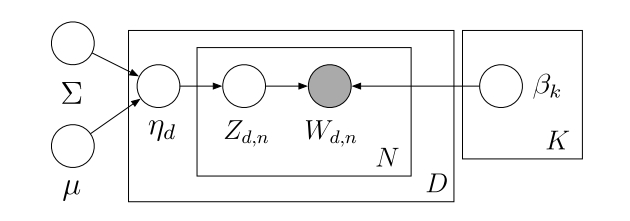
\includegraphics{figs/tm/clda_graphical_model.png}
\caption{}
\end{figure}

The joint distribution over all latent variables \(\theta\) and \(z\)
and observed data \(w\) is then

\[
p(\theta,z,w|\alpha,\beta) = \prod_d p(\eta_d|\mu,\Sigma) \prod_n p(w_{d,n}|z_{d,n},\beta) p(z_{d,n}|\eta_d)
\]

where

\[
\begin{aligned}
&p(\eta_d|\mu,\Sigma) = \frac{1}{\sqrt{(2\pi)^k |\Sigma|}} \exp [-\frac{1}{2}(\eta - \mu)^T \Sigma^{-1} (\eta - \mu)] \text{, (Multivariate Normal)}\\
&p(z_{d,n}|\eta_d) = \prod_n \prod_i \theta_i^{1[z_n=i]} \text{, (Multinomial)}\\
&p(w_{d,n}|z_{d,n},\beta) = \prod_v \prod_i \beta_{i,v}^{1[w_{d,n}=v,z_{d,n}=i]} \text{, (Multinomial)}
\end{aligned}
\]

\subsubsection{Multinomial Distribution in Exponential
Form}\label{multinomial-distribution-in-exponential-form}

Let's convert this multinomial \(p(z|\eta)\) into its natural parameter
form by exploiting the fact that it belongs to the exponential family.
The game is that we need to express this distribution in the form
\(p(x|\eta) = h(z) \exp [\eta^T \phi (x) - A(\eta)]\). Note, we'll work
with only one word \(n\) to simplify things, so

\[
\begin{aligned}
p(z|\theta) &= \prod_i^K \theta_i^{1[z_n=i]}\\
    &= \prod_i^K \exp [\log \theta_i^{1[z_n=i]}]\\
    &= \exp [\sum_i^K \log \theta_i^{1[z_n=i]}]\\
    &= \exp [\sum_i^K 1[z_n=i] \log \theta_i]
\end{aligned}
\]

Now we'll split the sum from all \(\sum_i^K\) to
\(\sum_i^{K-1} + 1-\sum_i^{K-1}\):

\[
\begin{aligned}
p(z|\theta) &= \exp [\sum_i 1[z_n=i] \log \theta_i]\\
    &= \exp [\sum_i^{K-1} 1[z_n=i] \log \theta_i + (1-\sum_i^{K-1} 1[z_n=i]) \log (1-\sum_i^{K-1}\theta_i)]
\end{aligned}
\]

Then we expand and group terms:

\[
\begin{aligned}
p(z|\theta) &= \exp [\sum_i^{K-1} 1[z_n=i] \log \theta_i + \log (1-\sum_i^{K-1}\theta_i) -\sum_i^{K-1} 1[z_n=i] \log (1-\sum_i^{K-1}\theta_i)]\\
    &= \exp [\sum_i^{K-1} 1[z_n=i] (\log \theta_i - \log (1-\sum_i^{K-1}\theta_i)) + \log (1-\sum_i^{K-1}\theta_i)]\\
    &= \exp [\sum_i^{K-1} 1[z_n=i] \log (\frac{\theta_i}{1-\sum_j^{K-1}\theta_j}) + \log (1-\sum_i^{K-1}\theta_i)]\\
\end{aligned}
\]

We can finally see the exponential form taking shape where

\[
\eta_i = \log(\frac{\theta_i}{1-\sum_j^{K-1}\theta_j}) = \log(\frac{\theta_i}{\theta_i})
\]

Now we can determine \(\theta_i\) by expressing this equation in terms
of \(\eta_i\):

\[
\begin{aligned}
\eta_i &= \log (\frac{\theta_i}{\theta_i})\\
\exp [\eta_i] &= \frac{\theta_i}{\theta_i}\\
\theta_i &= \theta_i \exp [\eta_i]\\
 &= (1-\sum_j^{K-1}\theta_j) \exp [\eta_i]\\
 &= \frac{1}{\frac{1}{(1-\sum_j^{K-1}\theta_j)}} \exp [\eta_i]
\end{aligned}
\]

For convenience, we'll assume \(\theta_i=\), so
\(\sum_i^{K-1}\theta_i = \sum_i^{K-1}\theta_i + \theta_i = \sum_i^{K-1}\theta_i + 0 = \sum_i^{K}\theta_i\).

\[
\begin{aligned}
\theta_i &= \frac{1}{\frac{1}{(1-\sum_j^{K-1}\theta_j)}} \exp [\eta_i]\\
&= \frac{1}{\frac{1}{(1-\sum_j^{K}\theta_j)}} \exp [\eta_i]
\end{aligned}
\]

Then we can take advantage of the following constraint:
\(\sum_j^K \theta_j = 1\), so

\[
\begin{aligned}
\theta_i &= \frac{1}{\frac{1}{(1-\sum_j^{K}\theta_j)}} \exp [\eta_i]\\
&= \frac{1}{\frac{\sum_j^K \theta_j}{(1-\sum_j^{K}\theta_j)}} \exp [\eta_i]\\
&= \frac{1}{\sum_j^K\frac{ \theta_j}{(1-\sum_j^{K}\theta_j)}} \exp [\eta_i]\\
&= \frac{1}{\sum_j^K \exp[\log \frac{ \theta_j}{(1-\sum_j^{K}\theta_j)}]} \exp [\eta_i]\\
&= \frac{1}{\sum_j^K \exp[\log \frac{ \theta_j}{\theta_i}]} \exp [\eta_i]\\
&= \frac{\exp [\eta_i]}{\sum_j^K \exp[\eta_j]}\\
\end{aligned}
\]

which is the softmax function. Now we can extract our natural
parameters:

\[
\begin{aligned}
h(z) &= 1\\
\phi(x) &= [1[z_n=1], ..., 1[z_n=K-1]]\\
\eta &= [\log(\frac{\theta_1}{1-\sum_j^{K-1}\theta_j}), ..., \log(\frac{\theta_{K-1}}{1-\sum_j^{K-1}\theta_j}),0]\\
    &= [\log(\frac{\theta_1}{\theta^K}),...,\log(\frac{\theta_{K-1}}{\theta^K}),0]
\end{aligned}
\]

We'll use the following notation \(\phi (x) := z\). For the cumulant,
let's again use \(\eta_i = \log (\frac{\theta_i}{\theta_i})\):

\[
\begin{aligned}
\eta_i &= \log (\frac{\theta_i}{\theta_i})\\
\theta_i &= \theta_i \exp [\eta_i]\\
\sum_i^{K-1} \theta_i &= \theta_i \sum_i^{K-1} \exp [\eta_i]\\
1-(1-\sum_i^{K-1} \theta_i) &= \theta_i \sum_i^{K-1} \exp [\eta_i]\\
1-\theta_i &= \theta_i \sum_i^{K-1} \exp [\eta_i]\\
1 &= \theta_i (1+\sum_i^{K-1} \exp [\eta_i]\\
\theta_i &= \frac{1}{1+\sum_i^{K-1} \exp [\eta_i]}\\
1-\sum_i^{K-1} \theta_i &= \frac{1}{1+\sum_i^{K-1} \exp [\eta_i]}
\end{aligned}
\]

Therefore

\[
\begin{aligned}
A(\eta) &= -\log (1-\sum_i^{K-1} \theta_i)\\
&= -\log (\frac{1}{1+\sum_i^{K-1} \exp [\eta_i]})\\
&= \log (1+\sum_i^{K-1} \exp [\eta_i])\\
\end{aligned}
\]

And if we assume that \(\theta_i = 0\), we have

\[
\begin{aligned}
A(\eta) &= \log (1+\sum_i^{K-1} \exp [\eta_i])\\
&= \log (\sum_i^{K} \exp [\eta_i])\\
\end{aligned}
\]

Thus, \(p(z|\eta)\) in its natural paramterization is

\[
\begin{aligned}
p(z_n|\eta) &= 1 \times \exp [\eta^T z_n - A(\eta)]\\
            &= \exp [\eta^T z_n - \log (\sum_i^{K} \exp [\eta_i])]
\end{aligned}
\]

\subsubsection{Variational EM}\label{variational-em}

Now, our variational distribution for CTM will be a again be a mean
field distribution where we assume complete independence between each
\(\eta\) and between all topic assignments \(z\), i.e., a fully factored
form. Note, unlike before, we're showing the variational distribution
for only one document:

\[
q(\eta,z|\lambda,\nu,\phi) = \prod_i q(\eta_i|\lambda_i,\nu_i^2) \prod_n q(z_n|\phi_n)
\]

where \(\phi\) is \(K \times N\), as before, and
\(\eta_i \thicksim \text{Normal}(\gamma_i,\nu_i)\) -- that is, each
\(\eta_i\) is distributed by its own \emph{univariate} Gaussian.

For the joint distribution over latent variables, we have

\[
\begin{aligned}
\log p&(w|\mu, \Sigma, \beta) \geq L(\gamma,\nu,\phi|\mu, \Sigma, \beta) \\
    &= \mathbb{E}_q [\log  p(\eta,z,w|\mu, \Sigma, \beta)] - \mathbb{E}_q [\log q(\eta,z)] \\
    &= \mathbb{E}_q [\log p(\eta|\mu,\Sigma)p(z|\theta)p(w|z,\beta)] - \mathbb{E}_q [\log q(\eta)q(z)]\\
    &= \mathbb{E}_q [\log p(\eta|\mu,\Sigma) + \log p(z|\eta) + \log p(w|z,\beta)] - \mathbb{E}_q [\log q(\eta) + \log q(z)]\\
    &= \mathbb{E}_q [\log p(\eta|\mu,\Sigma)] + \mathbb{E}_q [\log p(z|\eta)] + \mathbb{E}_q [\log p(w|z,\beta)] \\
    &\qquad - \mathbb{E}_q [\log q(\eta)] - \mathbb{E}_q[\log q(z)]\\
    &= \mathbb{E}_q [\log p(\eta|\mu,\Sigma)] + \mathbb{E}_q [\log p(z|\eta)] + \mathbb{E}_q [\log p(w|z,\beta)] + \mathbb{H}_q [\lambda,\nu^2] + \mathbb{H}_q[\phi]
\end{aligned} 
\]

\subsubsection{\texorpdfstring{Expectation of
\(p(w|z,\beta)\)}{Expectation of p(w\textbar{}z,\textbackslash{}beta)}}\label{expectation-of-pwzbeta-1}

This is analogous to LDA:

\[
\mathbb{E}_q [\log p(w|z,\beta)] = \sum_v \sum_i 1[w_{d,n}=v] \phi_{n,i} \log \beta_{i,v}
\]

\subsubsection{\texorpdfstring{Expectation of
\(p(z|\eta)\)}{Expectation of p(z\textbar{}\textbackslash{}eta)}}\label{expectation-of-pzeta}

In LDA, working with \(p(z|\theta)\) was simple because of the conjugacy
between Multinomial and Dirichlet distributions, respectively. Now,
however, we are working with a Normal prior, which is \emph{not}
conjugate with the Multinomial. Similar to before,
\(z_n \thicksim \text{Multinomial}(f(\eta))\). Now recall that
\(\eta_i \thicksim \text{Normal}(\gamma_i,\nu_i)\) and then mapped onto
the simplex via \(f(\eta_i)= \exp \eta_i / \sum_j \exp \eta_j\). You can
see this relationship by returning to the natural parameterization of
the Multinomial distribution \(p(z|\eta)\):

\[
\begin{aligned}
\log p(z|\eta) &= \log \exp [\eta^T z_n - \log (\sum_i^{K} \exp [\eta_i])]\\
    &= \eta^T z_n - \log (\sum_i^{K} \exp [\eta_i])\\
    &= \log \exp [\eta^T z_n] - \log (\sum_i^{K} \exp [\eta_i])\\
    &= \log [\frac{\exp [\eta^T z_n]}{\sum_i^{K} \exp [\eta_i]}]\\
\end{aligned}
\]

which shows \(\eta\) being mapped to the simplex. Now, let's derive the
expectation:

\[
\begin{aligned}
\mathbb{E}_q [\log p(z_n|\eta)] &= \mathbb{E}_q [\log \exp [\eta^T z_n - \log(\sum_i^{K} \exp [\eta_i])]] \\ 
    &= \mathbb{E}_q [\eta^T z_n - \log(\sum_i^{K} \exp [\eta_i])] \\ 
    &= \mathbb{E}_q [\eta^T z_n] - \mathbb{E}_q [\log(\sum_i^{K} \exp [\eta_i])] \\ 
\end{aligned}
\]

The left side is easy. Recall that \(z_n\) are simply indicator
functions for a particular topic assignment, so for a given document and
word \(n\), \(z_n\) is a K-vector of indicator values where the topic
\(k\) is equal to \(1\) and all other topics are \(0\). Its expectation
is the corresponding variational parameter \(\phi_{n,i}\), which is
simply a matrix of values that reflects the frequency in which a token
\(n\) takes on the topic assignment \(i\). Because \(\eta_i\) is a
Gaussian with mean \(\lambda_i\) that corresponds to topic \(i\), its
expectation is simply \(\lambda\). Thus, the expectation of
\(\eta^T z_n\) is simply the sum across tokens of the product between
the average prior value \(\lambda_i\) for token \(i\) and the number of
times token \(n\) was assigned to topic \(i\):

\[
\begin{aligned}
\mathbb{E}_q [\eta^T z_n] = \sum_n \sum_i \lambda_i \phi_{n,i} \\ 
\end{aligned}
\]

Giving us

\[
\begin{aligned}
\mathbb{E}_q [\log p(z_n|\eta)] &= \mathbb{E}_q [\eta^T z_n] - \mathbb{E}_q [\log(\sum_i^{K} \exp [\eta_i])]\\
    &= \sum_n \sum_i \lambda_i \phi_{n,i} - \mathbb{E}_q [\log(\sum_i^{K} \exp [\eta_i])] 
\end{aligned}
\]

The right side, on the other hand, is intractable, but we can introduce
an upper bound to \(\mathbb{E}_q [\log(\sum_i^{K} \exp [\eta_i])]\).
Think about it like this. For variational inference, we are maximizing a
lower bound of the log probability of our model. The term we are
focusing on is
\(\mathbb{E}_q [\eta^T z_n] - \mathbb{E}_q [\log(\sum_i^{K} \exp [\eta_i])]\),
which we'll rewrite as \(\mathbb{E}_q [A - B]\). We need to ensure that
our lower bound from the variational distribution remains the lower
bound. Therefore, our approximation of \(\mathbb{E}_q [A - B]\) must be
smaller, which would give us a smaller approximated lower bound and
hence smaller than the true lower bound. Since \(B\) is the part that is
intractable, we only need to approximate it, and not the left term. If
we increase \(B\), we'll consequently decrease our approximation of
\(\mathbb{E}_q [\log p(z_n|\eta)]\), giving us an approximated lower
bound that's smaller than the true lower bound, which is what we want.
Therefore, we need to find \(C\) such that
\(\mathbb{E}_q [A - B] \leq C\).

To find ``\(C\)'', we do the following. We'll approximate the
intractable sum as \(\log x \approx x-1\), which is the case when \(x\)
is around \(1\). Also, \(\log x\) is never greater than \(x-1\) and
hence \(x-1\) serves as a tight upper bound:

\begin{figure}[htbp]
\centering
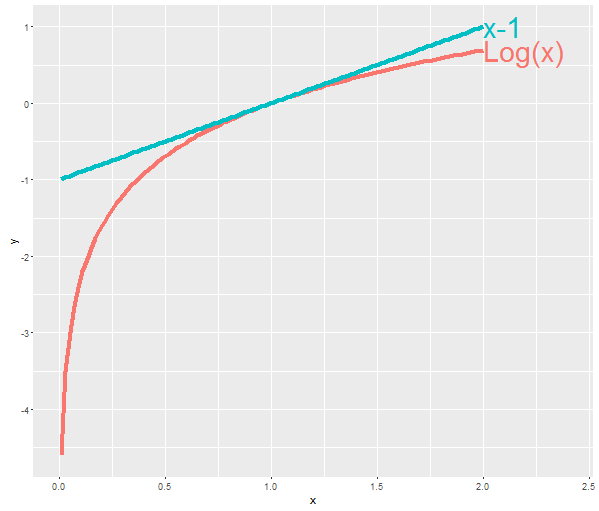
\includegraphics{figs/tm/xminus1.png}
\caption{}
\end{figure}

We will also introduce a new variational parameter \(\xi\).

\[
\begin{aligned}
\mathbb{E}_q [\log(\sum_i^{K} \exp [\eta_i])] &=  \mathbb{E}_q [\log(\xi \xi^{-1} \sum_i^{K} \exp [\eta_i])]\\
    &= \mathbb{E}_q [\log \xi + \log (\xi^{-1} \sum_i^{K} \exp [\eta_i])]\\
    &= \log \xi + \mathbb{E}_q [\log (\xi^{-1} \sum_i^{K} \exp [\eta_i])]\\
    &\leq \log \xi + \mathbb{E}_q [\xi^{-1} \sum_i^{K} \exp [\eta_i] - 1]\\
    &\leq \log \xi + \xi^{-1} \sum_i^{K} \mathbb{E}_q [\exp [\eta_i]] - 1\\
\end{aligned}
\]

And so we have our almost final form for this expectation:

\[
\begin{aligned}
\mathbb{E}_q [\log p(z_n|\eta)] &= \sum_n (\sum_i \lambda_i \phi_{n,i} - \mathbb{E}_q [\log(\sum_i^{K} \exp [\eta_i])])\\
    &=\sum_n (\sum_i \lambda_i \phi_{n,i} - \log \xi + \mathbb{E}_q [\log (\xi^{-1} \sum_i^{K} \exp [\eta_i])])\\
    &\geq \sum_n (\sum_i \lambda_i \phi_{n,i} - (\log \xi + \xi^{-1} \sum_i^{K} \mathbb{E}_q [\exp [\eta_i]] - 1))
\end{aligned}
\]

Now, because \(\eta_i \thicksim \text{Normal} (\lambda_i,\nu_i^2)\),
\(\mathbb{E}_q [\exp [\eta_i]] = \exp [\lambda_i + \nu_i^2 /2]\), which
allows us to write our final form:

\[
\begin{aligned}
\mathbb{E}_q [\log p(z_n|\eta)] &\geq \sum_n (\sum_i \lambda_i \phi_{n,i} - (\log \xi + \xi^{-1} \sum_i^{K} \mathbb{E}_q [\exp [\eta_i]] - 1))\\
&\geq \sum_n (\sum_i \lambda_i \phi_{n,i} - (\log \xi + \xi^{-1} \sum_i^{K} \exp [\lambda_i + \frac{\nu_i^2}{2}] - 1))\\
&\geq \sum_n (\sum_i \lambda_i \phi_{n,i} - \log \xi - \xi^{-1} \sum_i^{K} \exp [\lambda_i + \frac{\nu_i^2}{2}] + 1)
\end{aligned}
\]

\subsubsection{\texorpdfstring{Expectation of
\(p(\eta|\mu,\sigma)\)}{Expectation of p(\textbackslash{}eta\textbar{}\textbackslash{}mu,\textbackslash{}sigma)}}\label{expectation-of-petamusigma}

We know that
\(p(\eta|\mu,\Sigma) \thicksim \text{Normal}_i (\mu,\Sigma)\), so

\[
\begin{aligned}
\log p(\eta|\mu,\Sigma) &= \frac{1}{2} \log |\Sigma^{-1}| - \frac{K}{2} \log 2\pi - \frac{1}{2} \mathbb{E}_q [(\eta - \mu)^T \Sigma^{-1} (\eta - \mu)] 
\end{aligned}
\]

We can rewrite \((\eta - \mu)^T \Sigma^{-1} (\eta - \mu)\) in a more
manageable form. Using \(x^T A x = \tr(x^T A x) = \tr(A x^T x)\), we
have the following:

\[
\begin{aligned}
(\eta - \mu)^T \Sigma^{-1} (\eta - \mu) &= \tr(\Sigma^{-1}  (\eta - \mu)^T (\eta - \mu))\\
    &= \tr(\Sigma^{-1}  \sum_i (\eta_i - \mu) (\eta_i - \mu))\\
    &= \tr(\Sigma^{-1}  \sum_i (\eta_i + (\lambda_i - \lambda_i) - \mu) (\eta_i + (\lambda_i - \lambda_i) - \mu))\\
    &= \tr(\Sigma^{-1}  \sum_i (\eta_i + \lambda_i - \lambda_i - \mu) (\eta_i + \lambda_i - \lambda_i - \mu))\\
    &= \tr(\Sigma^{-1}  (\sum_i (\eta_i - \lambda_i)(\eta_i - \lambda_i ) + \sum_i (\lambda_i - \mu)(\lambda_i - \mu)))\\
    &= \tr(\Sigma^{-1}\sum_i (\eta_i - \lambda_i)(\eta_i - \lambda_i ) + \Sigma^{-1}\sum_i (\lambda_i - \mu)(\lambda_i - \mu))\\
    &= \tr(\Sigma^{-1}\sum_i (\eta_i - \lambda_i)(\eta_i - \lambda_i )) + \tr(\Sigma^{-1}\sum_i (\lambda_i - \mu)(\lambda_i - \mu))\\
    &= \tr(\Sigma^{-1}\sum_i (\eta_i - \lambda_i)^2) + \tr(\Sigma^{-1}(\lambda - \mu)(\lambda - \mu)^T)\\
    &= \tr(\Sigma^{-1}\sum_i (\eta_i - \lambda_i)^2) + (\lambda - \mu)^T\Sigma^{-1}(\lambda - \mu)
\end{aligned}
\]

Now, let's take the expectation:

\[
\begin{aligned}
\mathbb{E}_q [(\eta - \mu)^T &\Sigma^{-1} (\eta - \mu)] \\
    &= \mathbb{E}_q [\tr(\Sigma^{-1}\sum_i (\eta_i - \lambda_i)^2) + (\lambda - \mu)^T\Sigma^{-1}(\lambda - \mu)] \\
    &= \tr(\Sigma^{-1} \mathbb{E}_q[\sum_i (\eta_i - \lambda_i)^2]) + (\lambda - \mu)^T\Sigma^{-1}(\lambda - \mu) 
\end{aligned}
\]

where \(\mathbb{E}_q[\sum_i (\eta_i - \lambda_i)^2]\) is simply the
variance of \(eta\) -- i.e., \(\nu^2\) -- which we'll place on the
diagonal of a square matrix.

\[
\begin{aligned}
\mathbb{E}_q [(\eta - \mu)^T &\Sigma^{-1} (\eta - \mu)] \\
    &= \tr(\Sigma^{-1} \mathbb{E}_q[\sum_i (\eta_i - \lambda_i)^2]) + (\lambda - \mu)^T\Sigma^{-1}(\lambda - \mu) \\
    &= \tr(\text{diag}(\nu^2)\Sigma^{-1}) + (\lambda - \mu)^T\Sigma^{-1}(\lambda - \mu)
\end{aligned}
\]

Therefore,

\[
\begin{aligned}
\log p(\eta|\mu,\Sigma) &= \frac{1}{2} \log |\Sigma^{-1}| - \frac{K}{2} \log 2\pi - \frac{1}{2} \mathbb{E}_q [(\eta - \mu)^T \Sigma^{-1} (\eta - \mu)] \\
&= \frac{1}{2} \log |\Sigma^{-1}| - \frac{K}{2} \log 2\pi - \frac{1}{2} (\tr(\text{diag}(\nu^2)\Sigma^{-1}) + (\lambda - \mu)^T\Sigma^{-1}(\lambda - \mu))\\
&= \frac{1}{2} \log |\Sigma^{-1}| - \frac{K}{2} \log 2\pi - \frac{1}{2} (\tr(\text{diag}(\nu^2)\Sigma^{-1}) + (\lambda - \mu)^T\Sigma^{-1}(\lambda - \mu))\\
&= \frac{1}{2} \log |\Sigma^{-1}| - \frac{K}{2} \log 2\pi - \frac{1}{2} \tr(\text{diag}(\nu^2)\Sigma^{-1}) - \frac{1}{2}(\lambda - \mu)^T\Sigma^{-1}(\lambda - \mu)
\end{aligned}
\]

\subsubsection{\texorpdfstring{Entropy of \(\lambda\), \(\nu\), and
\(\phi\)}{Entropy of \textbackslash{}lambda, \textbackslash{}nu, and \textbackslash{}phi}}\label{entropy-of-lambda-nu-and-phi}

Again, we can look these up.

\[
\begin{aligned}
\mathbb{H}_q [\lambda,\nu^2] &= \frac{1}{2} \sum_i \log[2 \pi e \nu_i^2] \\
        &= \frac{1}{2} \sum_i  (\log 2\pi + 1 + \log \nu_i^2)\\
\mathbb{H}_q [\phi_{d,n}] &= -\sum_i \phi_{d,n,i} \log \phi_{d,n,i}
\end{aligned} 
\]

\subsubsection{Complete Objective
Function}\label{complete-objective-function-2}

Our objective function is then

\[
\begin{aligned}
\mathbb{E}_q &[\log  p(\eta,z,w|\mu, \Sigma, \beta)] - \mathbb{E}_q [\log q(\eta,z)] \\
    &= \mathbb{E}_q [\log p(\eta|\mu,\Sigma)] + \mathbb{E}_q [\log p(z|\eta)] + \mathbb{E}_q [\log p(w|z,\beta)] + \mathbb{H}_q [\lambda,\nu^2] + \mathbb{H}_q[\phi] \\
    &= \frac{1}{2} \log |\Sigma^{-1}| - \frac{K}{2} \log 2\pi - \frac{1}{2} \tr(\text{diag}(\nu^2)\Sigma^{-1}) - \frac{1}{2}(\lambda - \mu)^T\Sigma^{-1}(\lambda - \mu) \\
    &\qquad + \sum_n (\sum_i \lambda_i \phi_{n,i} - \log \xi - \xi^{-1} \sum_i^{K} \exp [\lambda_i + \frac{\nu_i^2}{2}] + 1) \\
    &\qquad + \sum_v \sum_i 1[w_{d,n}=v] \phi_{n,i} \log \beta_{i,v} \\
    &\qquad + \frac{1}{2} \sum_i  (\log 2\pi + 1 + \log \nu_i^2) - \sum_i \phi_{d,n,i} \log \phi_{d,n,i}
\end{aligned} 
\]

\subsubsection{Parameter Optimization}\label{parameter-optimization-2}

\paragraph{\texorpdfstring{Optimization for
\(\beta\)}{Optimization for \textbackslash{}beta}}\label{optimization-for-beta-1}

This is the same as LDA:

\[
\beta_{i,v} \propto \sum_n \sum_i \sum_v 1[w_n = v] \phi_{n,i}
\]

\paragraph{\texorpdfstring{Optimization for
\(\mu\)\}}{Optimization for \textbackslash{}mu\}}}\label{optimization-for-mu}

Extracting the terms involving \(\mu\), we have

\[
\begin{aligned}
\frac{\partial L}{\partial \mu} &= \frac{\partial}{\partial \mu}[- \frac{1}{2} \sum_d (\lambda_d - \mu)^T\Sigma^{-1}(\lambda_d - \mu)] \\
    &= \frac{\partial}{\partial \mu}[- \frac{1}{2}\sum_d (\lambda_d - \mu)^T\Sigma^{-1}(\lambda_d - \mu)] \\
    &= (-\frac{1}{2})(-2) \Sigma^{-1}\sum_d(\lambda_d-\mu)\\
    &= \Sigma^{-1}\sum_d(\lambda_d-\mu)
\end{aligned} 
\]

Set it to zero.

\[
\begin{aligned}
0 &= \Sigma^{-1}\sum_d(\lambda_d-\mu)\\
    &= \sum_d \lambda_d - \sum_d \mu \\
    &= \sum_d \lambda_d - D \mu \\
D \mu &= \sum_d \lambda_d \\
\mu &= \frac{1}{D} \sum_d \lambda_d
\end{aligned} 
\]

\paragraph{\texorpdfstring{Optimization for
\(\Sigma\)}{Optimization for \textbackslash{}Sigma}}\label{optimization-for-sigma}

Let's repeat the process, but for terms associated with \(\Sigma\):

\[
\begin{aligned}
\frac{\partial L}{\partial \Sigma} &= \frac{\partial}{\partial \Sigma}[\sum_d(-\frac{1}{2} \log |\Sigma| - \frac{1}{2} \tr(\text{diag}(\nu_d^2)\Sigma^{-1}) - \frac{1}{2}(\lambda_d - \mu)^T\Sigma^{-1}(\lambda_d - \mu))] \\
&= -\frac{1}{2}\frac{\partial}{\partial \Sigma} [\sum_d (\log |\Sigma| + \tr(\text{diag}(\nu_d^2)\Sigma^{-1}) + (\lambda_d - \mu)^T\Sigma^{-1}(\lambda_d - \mu))] \\
&= -\frac{1}{2}\frac{\partial}{\partial \Sigma} [D \log |\Sigma| + \tr(\sum_d\text{diag}(\nu_d^2)\Sigma^{-1}) + \sum_d(\lambda_d - \mu)^T\Sigma^{-1}(\lambda_d - \mu)] \\
&= -\frac{1}{2}(D \frac{\partial}{\partial \Sigma}[\log |\Sigma|] + \frac{\partial}{\partial \Sigma}[\tr(\sum_d\text{diag}(\nu_d^2)\Sigma^{-1})] \\
&\qquad + \frac{\partial}{\partial \Sigma}[\sum_d(\lambda_d - \mu)^T\Sigma^{-1}(\lambda_d - \mu)]) 
\end{aligned} 
\]

Let's first focus on
\(\frac{\partial}{\partial \Sigma} [\sum_d(\lambda_d - \mu)^T\Sigma^{-1}(\lambda_d - \mu)]\).
We can use the trace trick we saw above to make this derivative easier
to work with:

\[
\begin{aligned}
\frac{\partial}{\partial \Sigma} &[\sum_d(\lambda_d - \mu)^T\Sigma^{-1}(\lambda_d - \mu)] \\
&= \frac{\partial}{\partial \Sigma} [\tr(\sum_d(\lambda_d - \mu)^T\Sigma^{-1}(\lambda_d - \mu))]\\
&= \frac{\partial}{\partial \Sigma} [\tr(\sum_d(\lambda_d - \mu)(\lambda_d - \mu)^T\Sigma^{-1})]\\
&= \tr(\sum_d(\lambda_d - \mu)(\lambda_d - \mu)^T\frac{\partial}{\partial \Sigma}\Sigma^{-1})\\
&= \tr(\sum_d(\lambda_d - \mu)(\lambda_d - \mu)^T (-\Sigma^{-1}\partial \Sigma \Sigma^{-1} ))\\
&= \tr(-\sum_d(\lambda_d - \mu)(\lambda_d - \mu)^T \Sigma^{-1}\partial \Sigma \Sigma^{-1})
\end{aligned}
\]

Now, let's deal with
\(\frac{\partial}{\partial \Sigma}[\log |\Sigma|]\).

\[
\begin{aligned}
\frac{\partial}{\partial \Sigma}[\log |\Sigma|] &= \tr(\Sigma^{-1} \partial \Sigma)
\end{aligned}
\]

And finally,
\(\frac{\partial}{\partial \Sigma}[\tr(\sum_d\text{diag}(\nu_d^2)\Sigma^{-1})]\).

\[
\begin{aligned}
\frac{\partial}{\partial \Sigma}[\tr(\sum_d\text{diag}(\nu_d^2)\Sigma^{-1})] &= \tr(\sum_d\text{diag}(\nu_d^2) (-\Sigma^{-1}\partial \Sigma \Sigma^{-1} ))\\
&= \tr(-\sum_d\text{diag}(\nu_d^2) (\Sigma^{-1}\partial \Sigma \Sigma^{-1} ))
\end{aligned}
\]

Now let's replace these derivatives in our original equation.

\[
\begin{aligned}
\frac{\partial L}{\partial \Sigma} &= -\frac{1}{2}(D \frac{\partial}{\partial \Sigma}[\log |\Sigma|] + \frac{\partial}{\partial \Sigma}[\tr(\sum_d\text{diag}(\nu_d^2)\Sigma^{-1})] \\
&\qquad + \frac{\partial}{\partial \Sigma}[\sum_d(\lambda_d - \mu)^T\Sigma^{-1}(\lambda_d - \mu)])\\
&= -\frac{1}{2}(D \tr(\Sigma^{-1} \partial \Sigma) + \tr(-\sum_d\text{diag}(\nu_d^2) (\Sigma^{-1}\partial \Sigma \Sigma^{-1} )) \\
&\qquad + \tr(-\sum_d(\lambda_d - \mu)(\lambda_d - \mu)^T \Sigma^{-1}\partial \Sigma \Sigma^{-1}))\\
&= -\frac{1}{2}(\tr(D\Sigma^{-1} \partial \Sigma) + \tr(-\sum_d\text{diag}(\nu_d^2) (\Sigma^{-1}\partial \Sigma \Sigma^{-1} )) \\
&\qquad + \tr(-\sum_d(\lambda_d - \mu)(\lambda_d - \mu)^T \Sigma^{-1}\partial \Sigma \Sigma^{-1}))\\
&= -\frac{1}{2}(\tr(D\Sigma^{-1} \partial \Sigma - \sum_d\text{diag}(\nu_d^2) \Sigma^{-1}\partial \Sigma \Sigma^{-1}  \\
&\qquad - \sum_d(\lambda_d - \mu)(\lambda_d - \mu)^T \Sigma^{-1}\partial \Sigma \Sigma^{-1}))\\
\end{aligned} 
\]

Then we set this to zero and solve.

\[
\begin{aligned}
0 &= -\frac{1}{2}(\tr(D\Sigma^{-1} \partial \Sigma - \sum_d\text{diag}(\nu_d^2) \Sigma^{-1}\partial \Sigma \Sigma^{-1}  \\
&\qquad - \sum_d(\lambda_d - \mu)(\lambda_d - \mu)^T \Sigma^{-1}\partial \Sigma \Sigma^{-1}))\\
&= \tr(D\Sigma^{-1} \partial \Sigma - \sum_d\text{diag}(\nu_d^2) \Sigma^{-1}\partial \Sigma \Sigma^{-1}  \\
&\qquad - \sum_d(\lambda_d - \mu)(\lambda_d - \mu)^T \Sigma^{-1}\partial \Sigma \Sigma^{-1})\\
&= \tr(D\Sigma^{-1} \partial \Sigma) - \tr(\sum_d\text{diag}(\nu_d^2) \Sigma^{-1}\partial \Sigma \Sigma^{-1})  \\
&\qquad - \tr(\sum_d(\lambda_d - \mu)(\lambda_d - \mu)^T \Sigma^{-1}\partial \Sigma \Sigma^{-1})\\
&= \tr(D\Sigma^{-1} \partial \Sigma) - \tr(\sum_d\text{diag}(\nu_d^2) \Sigma^{-1}\partial \Sigma \Sigma^{-1})  \\
&\qquad - \tr(\sum_d(\lambda_d - \mu)(\lambda_d - \mu)^T \Sigma^{-1}\partial \Sigma \Sigma^{-1})\\
\end{aligned} 
\]

Then we exploit \(\tr(ABCD) = \tr(DABC)\).

\[
\begin{aligned}
\tr(D\Sigma^{-1} \partial \Sigma) &= \tr(\sum_d\text{diag}(\nu_d^2) \Sigma^{-1}\partial \Sigma \Sigma^{-1}) + \tr(\sum_d(\lambda_d + \mu)(\lambda_d - \mu)^T \Sigma^{-1}\partial \Sigma \Sigma^{-1})\\
&= \tr(\sum_d \Sigma^{-1}) \text{diag}(\nu_d^2) \Sigma^{-1}\partial \Sigma  + \tr(\sum_d \Sigma^{-1} (\lambda_d + \mu)(\lambda_d - \mu)^T \Sigma^{-1}\partial \Sigma)\\
D\Sigma^{-1} \partial \Sigma &= \sum_d \Sigma^{-1} \text{diag}(\nu_d^2) \Sigma^{-1}\partial \Sigma  + \sum_d \Sigma^{-1} (\lambda_d + \mu)(\lambda_d - \mu)^T \Sigma^{-1}\partial \Sigma\\
D\Sigma^{-1} \partial \Sigma &= (\sum_d \Sigma^{-1} \text{diag}(\nu_d^2) \Sigma^{-1}  + \sum_d \Sigma^{-1} (\lambda_d + \mu)(\lambda_d - \mu)^T \Sigma^{-1})\partial \Sigma\\
D\Sigma^{-1} &= \sum_d \Sigma^{-1} \text{diag}(\nu_d^2) \Sigma^{-1}  + \sum_d \Sigma^{-1} (\lambda_d + \mu)(\lambda_d - \mu)^T \Sigma^{-1}\\
D &= \sum_d \Sigma^{-1} \text{diag}(\nu_d^2)  + \sum_d \Sigma^{-1} (\lambda_d + \mu)(\lambda_d - \mu)^T\\
\Sigma D &= \sum_d \text{diag}(\nu_d^2)  + \sum_d (\lambda_d + \mu)(\lambda_d - \mu)^T\\
\Sigma &= \frac{1}{D}(\sum_d \text{diag}(\nu_d^2)  + (\lambda_d + \mu)(\lambda_d - \mu)^T)
\end{aligned}
\]

\paragraph{\texorpdfstring{Optimization for
\(\xi\)}{Optimization for \textbackslash{}xi}}\label{optimization-for-xi}

Isolating terms, we get

\[
\begin{aligned}
\frac{\partial L}{\partial \xi} &= \frac{\partial}{\partial \xi}[ - \log \xi - \xi^{-1} \sum_i^{K} \exp [\lambda_i + \frac{\nu_i^2}{2}]]\\
&= - \frac{1}{\xi} + \frac{1}{\xi^{2}} \sum_i^{K} \exp [\lambda_i + \frac{\nu_i^2}{2}]
\end{aligned}
\]

Then we set this equal to zero:

\[
\begin{aligned}
0 &= - \frac{1}{\xi} + \frac{1}{\xi^{2}} \sum_i^{K} \exp [\lambda_i + \frac{\nu_i^2}{2}]\\
\frac{1}{\xi} &= \frac{1}{\xi^{2}} \sum_i^{K} \exp [\lambda_i + \frac{\nu_i^2}{2}]\\
\xi &=  \sum_i^{K} \exp [\lambda_i + \frac{\nu_i^2}{2}]
\end{aligned}
\]

\paragraph{\texorpdfstring{Optimization for
\(\phi\)}{Optimization for \textbackslash{}phi}}\label{optimization-for-phi-2}

Again, isolating terms and adding the constraint
\(\sum_n \phi_{n,i} = 1\), we get

\[
\begin{aligned}
\frac{\partial L}{\partial \phi_{n,i}} &= \frac{\partial}{\partial \phi_{n,i}}[\gamma_i \phi_{n,i} + \sum_v 1[w_{n}=v]\phi_{n,i} \log \beta_{i,v} -\phi_{n,i} \log \phi_{n,i} + \zeta(\sum_n \phi_{n,i}-1)]\\
&= \gamma_i + \sum_v 1[w_{n}=v]\log \beta_{i,v} - \log \phi_{n,i} - 1 + \zeta
\end{aligned}
\]

which we set to zero

\[
\begin{aligned}
0 &= \gamma_i + \sum_v 1[w_{n}=v]\log \beta_{i,v} - \log \phi_{n,i} - 1 + \zeta\\
\log \phi_{n,i} &= \gamma_i + \sum_v 1[w_{n}=v]\log \beta_{i,v} - 1 + \zeta\\
\phi_{n,i} &= \exp[\gamma_i]\exp[\log \beta_{i,v}^{1[w_{n}=v]}]\exp[ - 1 + \zeta]\\
&= \exp[\gamma_i]\beta_{i,v}^{1[w_{n}=v]}\exp[ - 1 + \zeta]\\
&= \exp[ - 1 + \zeta]\beta_{i,v}^{1[w_{n}=v]}\exp[\gamma_i]\\
&= c_{n,i}\beta_{i,v}^{1[w_{n}=v]}\exp[\gamma_i]\\
&\propto \beta_{i,v}^{1[w_{n}=v]}\exp[\gamma_i]
\end{aligned}
\]

where \(c_{n,i}=\exp[ - 1 + \zeta]\). As in LDA, we will calculate
\(\phi\) and then normalize to satisfy this constraint.

\paragraph{\texorpdfstring{Optimization for
\(\lambda\)}{Optimization for \textbackslash{}lambda}}\label{optimization-for-lambda}

Isolating terms and rewriting some of the sums as vectors, we get the
following expression.

\[
\begin{aligned}
\frac{\partial L}{\partial \lambda} &= \frac{\partial}{\partial \lambda}[- \frac{1}{2}(\lambda - \mu)^T\Sigma^{-1}(\lambda - \mu) + \sum_n \sum_i \lambda_i \phi_{n,i} - \xi^{-1} \sum_n \sum_i^{K} \exp [\lambda_i + \frac{\nu_i^2}{2}]]\\
&= \frac{\partial}{\partial \lambda}[- \frac{1}{2}(\lambda - \mu)^T\Sigma^{-1}(\lambda - \mu) + \sum_n \lambda \phi_{n,\cdot} - \xi^{-1} \sum_n \exp [\lambda + \frac{\nu^2}{2}]]\\
&= \frac{\partial}{\partial \lambda}[- \frac{1}{2}(\lambda - \mu)^T\Sigma^{-1}(\lambda - \mu) + \sum_n \lambda \phi_{n,\cdot} - \frac{N}{\xi} \exp [\lambda + \frac{\nu^2}{2}]]\\
\end{aligned} 
\]

Now, let's compute the derivative:

\[
\begin{aligned}
\frac{\partial L}{\partial \lambda} &= \frac{\partial}{\partial \lambda}[- \frac{1}{2}(\lambda - \mu)^T\Sigma^{-1}(\lambda - \mu) + \sum_n \lambda \phi_{n,\cdot} - \frac{N}{\xi} \exp [\lambda + \frac{\nu^2}{2}]]\\
&= - \frac{1}{2}(2\Sigma^{-1}(\lambda - \mu)) + \sum_n \phi_{n,\cdot} - \frac{N}{\xi} \exp [\lambda + \frac{\nu^2}{2}]\\
&= - \Sigma^{-1}(\lambda - \mu) + \sum_n \phi_{n,\cdot} - \frac{N}{\xi} \exp [\lambda + \frac{\nu^2}{2}]
\end{aligned} 
\]

This cannot be solved analytically, but we can apply gradient descent.

\paragraph{\texorpdfstring{Optimization for
\(\nu^2\)}{Optimization for \textbackslash{}nu\^{}2}}\label{optimization-for-nu2}

For our last optimization, we'll again isolate terms. Let's rewrite
\(\nu_i^2\) as \(\delta_i := \nu_i^2\) to prevent confusion.

\[
\begin{aligned}
\frac{\partial L}{\partial \delta}  &= \frac{\partial}{\partial \delta_i}[- \frac{1}{2} \delta_i\Sigma_{ii}^{-1} 
    - \xi^{-1} \sum_n \exp [\lambda_i + \frac{\delta_i}{2}] + \frac{1}{2} \log \delta_i ]\\
    &= \frac{\partial}{\partial \delta_i}[- \frac{1}{2} \delta_i\Sigma_{ii}^{-1}
    - \frac{N}{\xi}\exp [\lambda_i + \frac{\delta_i}{2}] + \frac{1}{2} \log \delta_i ]\\
    &= -\frac{1}{2}\Sigma_{ii}^{-1} - \frac{N}{2\xi}\exp [\lambda_i + \frac{\delta_i}{2}] + \frac{1}{2\delta}\\
\end{aligned} 
\]

which, in terms of \(\nu^2\), is

\[
\begin{aligned}
\frac{\partial L}{\partial \nu^2} &= -\frac{1}{2}\Sigma_{ii}^{-1}   - \frac{N}{2\xi}\exp [\lambda_i + \frac{\nu^2}{2}] + \frac{1}{2 \nu^2}\\
\end{aligned} 
\]

Like \(\frac{\partial L}{\partial \lambda}\), this cannot be solved
analytically. We can use Newton's method, but we first need to solve for
the Hessian:

\[
\begin{aligned}
\frac{\partial^2 L}{\partial \delta^2}  &= \frac{\partial}{\partial \delta_i}[-\frac{1}{2}\Sigma_{ii}^{-1}  - \frac{N}{2\xi}\exp [\lambda_i + \frac{\delta_i}{2}] + \frac{1}{2\delta}]\\
&= - \frac{N}{4\xi}\exp [\lambda_i + \frac{\delta_i}{2}] - \frac{1}{2\delta^2}\\
\end{aligned} 
\]

which in terms of \(\nu^2\) is

\[
\begin{aligned}
\frac{\partial^2 L}{\partial (\nu^2)^2} &= - \frac{N}{4\xi}\exp [\lambda_i + \frac{\nu^2}{2}] - \frac{1}{2(\nu^2)^2}\\
\end{aligned} 
\]

\subsection{Dirichlet Distribution}\label{dirichlet-distribution}

\begin{Shaded}
\begin{Highlighting}[]
\NormalTok{dsim <-}\StringTok{ }\NormalTok{function(}\DataTypeTok{alpha=}\KeywordTok{c}\NormalTok{(}\DecValTok{1}\NormalTok{,}\DecValTok{1}\NormalTok{,}\DecValTok{1}\NormalTok{),draws)\{}
  
  \NormalTok{if (}\KeywordTok{length}\NormalTok{(alpha)==}\DecValTok{1}\NormalTok{) alpha <-}\StringTok{ }\KeywordTok{rep}\NormalTok{(alpha,}\DecValTok{3}\NormalTok{)}
  
  \NormalTok{elements <-}\StringTok{ }\KeywordTok{length}\NormalTok{(alpha)}
  
  \NormalTok{dis <-}\StringTok{ }\KeywordTok{rdirichlet}\NormalTok{(draws, alpha)}
  \NormalTok{disz <-}\StringTok{ }\KeywordTok{ddirichlet}\NormalTok{(dis, alpha)}
  \NormalTok{triangle <-}\StringTok{ }\KeywordTok{data.frame}\NormalTok{(}\KeywordTok{cbind}\NormalTok{(dis,disz))}
  \KeywordTok{names}\NormalTok{(triangle) <-}\StringTok{ }\KeywordTok{c}\NormalTok{(}\StringTok{"A"}\NormalTok{,}\StringTok{"B"}\NormalTok{,}\StringTok{"C"}\NormalTok{,}\StringTok{"d"}\NormalTok{)}
  
  \NormalTok{df <-}\StringTok{ }\KeywordTok{data.frame}\NormalTok{(}\StringTok{"Atom"}\NormalTok{=}\KeywordTok{as.factor}\NormalTok{(}\KeywordTok{rep}\NormalTok{(LETTERS[}\DecValTok{1}\NormalTok{:elements], }\DataTypeTok{each=}\NormalTok{draws)),}
                   \StringTok{"Probability"}\NormalTok{=}\KeywordTok{matrix}\NormalTok{(dis,}\DataTypeTok{ncol=}\DecValTok{1}\NormalTok{),}
                   \StringTok{"Draw"}\NormalTok{=}\KeywordTok{as.factor}\NormalTok{(}\KeywordTok{rep}\NormalTok{(}\DecValTok{1}\NormalTok{:draws,elements)))}
  
  \NormalTok{p <-}\StringTok{  }\KeywordTok{ggplot}\NormalTok{(}\KeywordTok{subset}\NormalTok{(df,Draw %in%}\StringTok{ }\DecValTok{1}\NormalTok{:}\DecValTok{15}\NormalTok{), }\KeywordTok{aes}\NormalTok{(}\DataTypeTok{x=}\NormalTok{Atom,}\DataTypeTok{y=}\NormalTok{Probability,}\DataTypeTok{ymin=}\DecValTok{0}\NormalTok{,}\DataTypeTok{ymax=}\NormalTok{Probability)) +}
\StringTok{    }\KeywordTok{geom_linerange}\NormalTok{(}\DataTypeTok{colour=}\StringTok{"Blue"}\NormalTok{,}\DataTypeTok{size=}\FloatTok{1.5}\NormalTok{) +}
\StringTok{    }\KeywordTok{geom_point}\NormalTok{(}\DataTypeTok{colour=}\StringTok{"Blue"}\NormalTok{,}\DataTypeTok{size=}\DecValTok{4}\NormalTok{) +}
\StringTok{    }\KeywordTok{scale_y_continuous}\NormalTok{(}\DataTypeTok{lim=}\KeywordTok{c}\NormalTok{(}\DecValTok{0}\NormalTok{,}\DecValTok{1}\NormalTok{)) +}
\StringTok{    }\KeywordTok{facet_wrap}\NormalTok{(~Draw,}\DataTypeTok{ncol=}\DecValTok{5}\NormalTok{) +}
\StringTok{    }\KeywordTok{theme}\NormalTok{(}\DataTypeTok{panel.background =} \KeywordTok{element_rect}\NormalTok{(),}
          \DataTypeTok{title=}\KeywordTok{element_text}\NormalTok{(}\DataTypeTok{size=}\DecValTok{20}\NormalTok{),}
          \DataTypeTok{strip.text=}\KeywordTok{element_text}\NormalTok{(}\DataTypeTok{size=}\DecValTok{13}\NormalTok{),}
          \DataTypeTok{axis.text=}\KeywordTok{element_text}\NormalTok{(}\DataTypeTok{size=}\DecValTok{13}\NormalTok{),}
          \DataTypeTok{axis.title=}\KeywordTok{element_text}\NormalTok{(}\DataTypeTok{size=}\DecValTok{18}\NormalTok{,}\DataTypeTok{face=}\StringTok{"bold"}\NormalTok{)) +}
\StringTok{    }\KeywordTok{ggtitle}\NormalTok{(}\KeywordTok{bquote}\NormalTok{(alpha ==}\StringTok{ }\NormalTok{(.(}\KeywordTok{paste}\NormalTok{(alpha,}\DataTypeTok{collapse=}\StringTok{" "}\NormalTok{)))))}
  
  \NormalTok{if (elements==}\DecValTok{3}\NormalTok{)\{}
    \NormalTok{q <-}\StringTok{    }\KeywordTok{ggtern}\NormalTok{(}\DataTypeTok{data=}\NormalTok{triangle,}\KeywordTok{aes}\NormalTok{(}\DataTypeTok{x=}\NormalTok{C,}\DataTypeTok{y=}\NormalTok{A,}\DataTypeTok{z=}\NormalTok{B)) +}
\StringTok{      }\KeywordTok{geom_density_tern}\NormalTok{(}\KeywordTok{aes}\NormalTok{(}\DataTypeTok{weight=}\NormalTok{d,}\DataTypeTok{color=}\NormalTok{..level..),}\DataTypeTok{size=}\FloatTok{1.2}\NormalTok{) +}
\StringTok{      }\KeywordTok{geom_point}\NormalTok{(}\DataTypeTok{color=}\StringTok{"black"}\NormalTok{,}\DataTypeTok{size=}\DecValTok{4}\NormalTok{,}\DataTypeTok{alpha=}\NormalTok{.}\DecValTok{5}\NormalTok{) +}
\StringTok{      }\KeywordTok{scale_color_gradient}\NormalTok{(}\DataTypeTok{low=}\StringTok{"red"}\NormalTok{,}\DataTypeTok{high=}\StringTok{"white"}\NormalTok{) +}\StringTok{ }
\StringTok{      }\KeywordTok{theme_rgbw}\NormalTok{() +}
\StringTok{      }\KeywordTok{theme}\NormalTok{(}\DataTypeTok{panel.background =} \KeywordTok{element_rect}\NormalTok{(),}
            \DataTypeTok{tern.axis.arrow.text =}\KeywordTok{element_text}\NormalTok{(}\DataTypeTok{size=}\DecValTok{28}\NormalTok{,}\DataTypeTok{face=}\StringTok{"bold"}\NormalTok{),}
            \DataTypeTok{tern.axis.text=}\KeywordTok{element_text}\NormalTok{(}\DataTypeTok{size=}\DecValTok{18}\NormalTok{)}
            \NormalTok{) +}
\StringTok{      }\KeywordTok{guides}\NormalTok{(}\DataTypeTok{color=}\OtherTok{FALSE}\NormalTok{)}
    
    \KeywordTok{print}\NormalTok{(}\KeywordTok{plot_grid}\NormalTok{(q,p,}\DataTypeTok{ncol=}\DecValTok{2}\NormalTok{))}
  \NormalTok{\} else \{}
    \KeywordTok{print}\NormalTok{(p)}
  \NormalTok{\}}
\NormalTok{\}}
\end{Highlighting}
\end{Shaded}

\begin{Shaded}
\begin{Highlighting}[]
\KeywordTok{dsim}\NormalTok{(}\DecValTok{1}\NormalTok{,}\DataTypeTok{draws=}\DecValTok{100}\NormalTok{)}
\end{Highlighting}
\end{Shaded}

\includegraphics{11_topicmodels_files/figure-latex/unnamed-chunk-5-1.pdf}

\begin{Shaded}
\begin{Highlighting}[]
\KeywordTok{dsim}\NormalTok{(}\KeywordTok{c}\NormalTok{(}\DecValTok{1}\NormalTok{,}\DecValTok{10}\NormalTok{,}\DecValTok{1}\NormalTok{),}\DataTypeTok{draws=}\DecValTok{100}\NormalTok{)}
\end{Highlighting}
\end{Shaded}

\includegraphics{11_topicmodels_files/figure-latex/unnamed-chunk-6-1.pdf}

\begin{Shaded}
\begin{Highlighting}[]
\KeywordTok{dsim}\NormalTok{(.}\DecValTok{05}\NormalTok{,}\DataTypeTok{draws=}\DecValTok{100}\NormalTok{)}
\end{Highlighting}
\end{Shaded}

\includegraphics{11_topicmodels_files/figure-latex/unnamed-chunk-7-1.pdf}

\section{Machine Learning}\label{ml}

\subsection{Cross Valdiation}\label{cross-valdiation}

Proof that k-fold CV has less variance around the mean than LOOCV --
better for k-fold CV.

\subsubsection{LOOCV}\label{loocv}

\begin{Shaded}
\begin{Highlighting}[]
\NormalTok{N =}\StringTok{ }\DecValTok{1000}    \CommentTok{# data size}
\NormalTok{p =}\StringTok{ }\NormalTok{.}\DecValTok{10} \CommentTok{# probability of a misclassification}

\KeywordTok{set.seed}\NormalTok{(}\DecValTok{100}\NormalTok{)}
\NormalTok{d1 <-}\StringTok{ }\KeywordTok{rbinom}\NormalTok{(N,}\DecValTok{1}\NormalTok{,p) }\CommentTok{# bernoulli sampling: sample 1, check if it's a match}
\KeywordTok{mean}\NormalTok{(d1)}
\end{Highlighting}
\end{Shaded}

\begin{verbatim}
## [1] 0.113
\end{verbatim}

\begin{Shaded}
\begin{Highlighting}[]
\KeywordTok{mean}\NormalTok{(d1)*(}\DecValTok{1}\NormalTok{-}\KeywordTok{mean}\NormalTok{(d1))   }\CommentTok{# var}
\end{Highlighting}
\end{Shaded}

\begin{verbatim}
## [1] 0.100231
\end{verbatim}

\begin{Shaded}
\begin{Highlighting}[]
\KeywordTok{var}\NormalTok{(d1)}
\end{Highlighting}
\end{Shaded}

\begin{verbatim}
## [1] 0.1003313
\end{verbatim}

10-fold CV

\begin{Shaded}
\begin{Highlighting}[]
\NormalTok{k =}\StringTok{ }\DecValTok{10}              \CommentTok{# number of CV replications}
\NormalTok{n =}\StringTok{ }\NormalTok{N/k             }\CommentTok{# sample size for each k from data N}
\KeywordTok{set.seed}\NormalTok{(}\DecValTok{100}\NormalTok{)}
\NormalTok{d2 <-}\StringTok{ }\KeywordTok{rbinom}\NormalTok{(N,n,p)/n       }\CommentTok{# binomial sampling: from 1000, }
                    \CommentTok{# sample 100, sum number that are wrong of 100, }
                    \CommentTok{# divide by sample size to get error rate}
\KeywordTok{mean}\NormalTok{(d2)}
\end{Highlighting}
\end{Shaded}

\begin{verbatim}
## [1] 0.10191
\end{verbatim}

\begin{Shaded}
\begin{Highlighting}[]
\NormalTok{(k/N)*}\KeywordTok{mean}\NormalTok{(d2)*(}\DecValTok{1}\NormalTok{-}\KeywordTok{mean}\NormalTok{(d2)) }\CommentTok{# var}
\end{Highlighting}
\end{Shaded}

\begin{verbatim}
## [1] 0.0009152435
\end{verbatim}

\begin{Shaded}
\begin{Highlighting}[]
\KeywordTok{var}\NormalTok{(d2)}
\end{Highlighting}
\end{Shaded}

\begin{verbatim}
## [1] 0.0009229749
\end{verbatim}

note that 10xCV var is \textless{} LOOCV var.

\subsection{Naive Bayes}\label{naive-bayes}

\begin{Shaded}
\begin{Highlighting}[]
\NormalTok{sex <-}\StringTok{ }\KeywordTok{rep}\NormalTok{(}\KeywordTok{c}\NormalTok{(}\StringTok{"M"}\NormalTok{,}\StringTok{"F"}\NormalTok{),}\DataTypeTok{each=}\DecValTok{4}\NormalTok{)               }\CommentTok{# feature 1}
\NormalTok{h <-}\StringTok{ }\KeywordTok{c}\NormalTok{(}\DecValTok{6}\NormalTok{,}\FloatTok{5.92}\NormalTok{,}\FloatTok{5.58}\NormalTok{,}\FloatTok{5.92}\NormalTok{,}\DecValTok{5}\NormalTok{,}\FloatTok{5.5}\NormalTok{,}\FloatTok{5.42}\NormalTok{,}\FloatTok{5.75}\NormalTok{)        }\CommentTok{# feature 2}
\NormalTok{w <-}\StringTok{ }\KeywordTok{c}\NormalTok{(}\DecValTok{180}\NormalTok{,}\DecValTok{190}\NormalTok{,}\DecValTok{170}\NormalTok{,}\DecValTok{165}\NormalTok{,}\DecValTok{100}\NormalTok{,}\DecValTok{150}\NormalTok{,}\DecValTok{130}\NormalTok{,}\DecValTok{150}\NormalTok{)     }\CommentTok{# feature 3}
\NormalTok{f <-}\StringTok{ }\KeywordTok{c}\NormalTok{(}\DecValTok{12}\NormalTok{,}\DecValTok{11}\NormalTok{,}\DecValTok{12}\NormalTok{,}\DecValTok{10}\NormalTok{,}\DecValTok{6}\NormalTok{,}\DecValTok{8}\NormalTok{,}\DecValTok{7}\NormalTok{,}\DecValTok{9}\NormalTok{)             }\CommentTok{# feature 4}

\NormalTok{df1 <-}\StringTok{ }\KeywordTok{data.frame}\NormalTok{(sex,h,w,f)}
\NormalTok{uh <-}\StringTok{ }\KeywordTok{tapply}\NormalTok{(df1$h,df1$sex,mean)}
\NormalTok{uf <-}\StringTok{ }\KeywordTok{tapply}\NormalTok{(df1$f,df1$sex,mean)}
\NormalTok{uw <-}\StringTok{ }\KeywordTok{tapply}\NormalTok{(df1$w,df1$sex,mean)}
\NormalTok{sh <-}\StringTok{ }\KeywordTok{tapply}\NormalTok{(df1$h,df1$sex,sd)}
\NormalTok{sf <-}\StringTok{ }\KeywordTok{tapply}\NormalTok{(df1$f,df1$sex,sd)}
\NormalTok{sw <-}\StringTok{ }\KeywordTok{tapply}\NormalTok{(df1$w,df1$sex,sd)}

\NormalTok{new <-}\StringTok{ }\KeywordTok{data.frame}\NormalTok{(}\StringTok{"h"}\NormalTok{=}\DecValTok{6}\NormalTok{,}\StringTok{"w"}\NormalTok{=}\DecValTok{130}\NormalTok{,}\StringTok{"f"}\NormalTok{=}\DecValTok{8}\NormalTok{)}

\NormalTok{ps <-}\StringTok{ }\KeywordTok{table}\NormalTok{(df1$sex)/}\KeywordTok{length}\NormalTok{(df1$sex)    }\CommentTok{# P(F) P(M)}
\NormalTok{phgs <-}\StringTok{ }\KeywordTok{dnorm}\NormalTok{(new$h,uh,sh)          }\CommentTok{# P(h|F) P(h|M)}
\NormalTok{pwgs <-}\StringTok{ }\KeywordTok{dnorm}\NormalTok{(new$w,uw,sw)          }\CommentTok{# P(h|F) P(h|M)}
\NormalTok{pfgs <-}\StringTok{ }\KeywordTok{dnorm}\NormalTok{(new$f,uf,sf)          }\CommentTok{# P(h|F) P(h|M)}

\NormalTok{postf <-}\StringTok{ }\NormalTok{ps[}\DecValTok{1}\NormalTok{]*phgs[}\DecValTok{1}\NormalTok{]*pwgs[}\DecValTok{1}\NormalTok{]*pfgs[}\DecValTok{1}\NormalTok{]  }\CommentTok{# P(sex|h,w,f) = P(sex)*P(h|sex)*P(w|sex)*P(f|sex)}
\NormalTok{postm <-}\StringTok{ }\NormalTok{ps[}\DecValTok{2}\NormalTok{]*phgs[}\DecValTok{2}\NormalTok{]*pwgs[}\DecValTok{2}\NormalTok{]*pfgs[}\DecValTok{2}\NormalTok{]}

\NormalTok{if (postm >}\StringTok{ }\NormalTok{postf) }\StringTok{"M"} \NormalTok{else }\StringTok{"F"}
\end{Highlighting}
\end{Shaded}

\begin{verbatim}
## [1] "F"
\end{verbatim}

\subsection{SVM}\label{svm}

\begin{Shaded}
\begin{Highlighting}[]
\KeywordTok{data}\NormalTok{(iris)}
\NormalTok{train <-}\StringTok{ }\NormalTok{iris}
\NormalTok{train$y <-}\KeywordTok{ifelse}\NormalTok{(train[,}\DecValTok{5}\NormalTok{]==}\StringTok{"setosa"}\NormalTok{, }\DecValTok{1}\NormalTok{, -}\DecValTok{1}\NormalTok{)}

\NormalTok{train <-}\StringTok{ }\NormalTok{train[}\KeywordTok{order}\NormalTok{(train$y, }\DataTypeTok{decreasing=}\OtherTok{TRUE}\NormalTok{),]}

\NormalTok{X <-}\StringTok{ }\KeywordTok{as.matrix}\NormalTok{(train[,}\KeywordTok{c}\NormalTok{(}\StringTok{"Petal.Length"}\NormalTok{, }\StringTok{"Petal.Width"}\NormalTok{)])}
\NormalTok{y <-}\StringTok{ }\KeywordTok{as.matrix}\NormalTok{(train$y)}
\NormalTok{n <-}\StringTok{ }\KeywordTok{dim}\NormalTok{(X)[}\DecValTok{1}\NormalTok{]}
\end{Highlighting}
\end{Shaded}

\[
\begin{aligned}
\max \alpha &W(\alpha) = \sum{\alpha_1} - -.5 \sum{y_i y_j \alpha_i \alpha_j x_i^T x_j}\\
             &\text{s.t.} \quad \alpha_i \ge 0\\
             &\text{s.t.} \quad \sum_{\alpha_i * y_i} = 0
\end{aligned}
\]

is equivalent to

\[
\begin{aligned}
\min \alpha - &\alpha + 0.5 \alpha^T * H * \alpha\\
             &\text{s.t.} \quad \alpha \ge 0\\
             &\text{s.t.} \quad A \alpha \le 0\\
             &\text{where} \quad H(i,j) = y_i y_j x_i^T x_j\\
             &\text{where} \quad A = y^T\\
             &\text{note} \quad \max z \equiv \min -z
\end{aligned}
\]

And ipop is

\[
\begin{aligned}
\min_\alpha c &\alpha + 0.5 x^T H x\\
             &\text{s.t.} \quad b \le A \alpha \le b + r\\
             &\text{s.t.} \quad l \le \alpha \le u\\
             &\text{thus} \quad c=-1\\
             &\text{thus} \quad u = \infty, l=0 \quad \text{but will set $u$ to a large number}\\
             &\text{thus} \quad b=0, r=0 \quad \text{to remove this contraint}
\end{aligned}
\]

\begin{Shaded}
\begin{Highlighting}[]
\NormalTok{H <-}\StringTok{ }\KeywordTok{matrix}\NormalTok{(}\OtherTok{NA}\NormalTok{,n,n)}
\NormalTok{for (i in }\DecValTok{1}\NormalTok{:n)\{}
  \NormalTok{for (j in }\DecValTok{1}\NormalTok{:n)\{}
    \NormalTok{H[i,j] <-}\StringTok{ }\NormalTok{y[i]*y[j]*}\KeywordTok{t}\NormalTok{(X[i,])%*%X[j,]}
  \NormalTok{\}}
\NormalTok{\}}

\NormalTok{A <-}\StringTok{ }\KeywordTok{t}\NormalTok{(y)}
\NormalTok{c <-}\StringTok{ }\KeywordTok{matrix}\NormalTok{(}\KeywordTok{rep}\NormalTok{(-}\DecValTok{1}\NormalTok{,n))}
\NormalTok{l <-}\StringTok{ }\KeywordTok{matrix}\NormalTok{(}\KeywordTok{rep}\NormalTok{(}\DecValTok{0}\NormalTok{,n))}
\NormalTok{b <-}\StringTok{ }\DecValTok{0}
\NormalTok{u <-}\StringTok{ }\KeywordTok{matrix}\NormalTok{(}\KeywordTok{rep}\NormalTok{(}\FloatTok{1e5}\NormalTok{,n))}
\NormalTok{r <-}\StringTok{ }\DecValTok{0}

\NormalTok{alpha <-}\StringTok{ }\KeywordTok{primal}\NormalTok{(}\KeywordTok{ipop}\NormalTok{(c,H,A,b,l,u,r))}

\NormalTok{nonzero <-}\StringTok{ }\KeywordTok{which}\NormalTok{(}\KeywordTok{abs}\NormalTok{(alpha) >}\StringTok{ }\FloatTok{1e-5}\NormalTok{)}
\NormalTok{w <-}\StringTok{ }\KeywordTok{matrix}\NormalTok{(}\OtherTok{NA}\NormalTok{,}\DataTypeTok{nrow=}\KeywordTok{length}\NormalTok{(nonzero),}\DataTypeTok{ncol=}\KeywordTok{ncol}\NormalTok{(X))}
\NormalTok{for (i in }\KeywordTok{seq_along}\NormalTok{(nonzero))\{}
  \NormalTok{w[i,]  <-}\StringTok{ }\NormalTok{alpha[nonzero[i]]*y[nonzero[i]]*X[nonzero[i],]}
\NormalTok{\}}
\NormalTok{w <-}\StringTok{ }\KeywordTok{colSums}\NormalTok{(w)}

\NormalTok{b0 <-}\StringTok{ }\NormalTok{-(}\KeywordTok{max}\NormalTok{(}\KeywordTok{sapply}\NormalTok{(}\DecValTok{1}\NormalTok{:}\KeywordTok{sum}\NormalTok{(y==-}\DecValTok{1}\NormalTok{), function(i) }\KeywordTok{matrix}\NormalTok{(w,}\DataTypeTok{ncol=}\DecValTok{2}\NormalTok{) %*%}\StringTok{ }\NormalTok{X[y==-}\DecValTok{1}\NormalTok{,][i,])) +}\StringTok{ }\KeywordTok{min}\NormalTok{(}\KeywordTok{sapply}\NormalTok{(}\DecValTok{1}\NormalTok{:}\KeywordTok{sum}\NormalTok{(y==}\DecValTok{1}\NormalTok{), function(i) }\KeywordTok{matrix}\NormalTok{(w,}\DataTypeTok{ncol=}\DecValTok{2}\NormalTok{) %*%}\StringTok{ }\NormalTok{X[y==}\DecValTok{1}\NormalTok{,][i,])))/}\DecValTok{2}

\NormalTok{slope <-}\StringTok{ }\NormalTok{-w[}\DecValTok{1}\NormalTok{]/w[}\DecValTok{2}\NormalTok{]}
\NormalTok{intercept <-}\StringTok{ }\NormalTok{-b0/w[}\DecValTok{2}\NormalTok{]}

\KeywordTok{plot}\NormalTok{(X,}\DataTypeTok{pch=}\DecValTok{19}\NormalTok{,}\DataTypeTok{col=}\KeywordTok{ifelse}\NormalTok{(}\DecValTok{1}\NormalTok{:n %in%}\StringTok{ }\NormalTok{nonzero,}\StringTok{"green"}\NormalTok{,}\StringTok{"black"}\NormalTok{)) }\CommentTok{# green ~ support vectors}
\KeywordTok{abline}\NormalTok{(intercept,slope,}\DataTypeTok{col=}\StringTok{"red"}\NormalTok{)}
\end{Highlighting}
\end{Shaded}

\includegraphics{12_machinelearning_files/figure-latex/unnamed-chunk-7-1.pdf}

\begin{Shaded}
\begin{Highlighting}[]
\NormalTok{sigma =}\StringTok{ }\DecValTok{1}
\NormalTok{rbf <-}\StringTok{ }\KeywordTok{rbfdot}\NormalTok{(}\DataTypeTok{sigma =} \NormalTok{sigma)}
\NormalTok{H_rbf <-}\StringTok{ }\KeywordTok{kernelMatrix}\NormalTok{(rbf,X)}
\end{Highlighting}
\end{Shaded}

\subsubsection{Manual rbf kernal}\label{manual-rbf-kernal}

\begin{Shaded}
\begin{Highlighting}[]
\NormalTok{XtX <-}\StringTok{ }\NormalTok{X%*%}\KeywordTok{t}\NormalTok{(X) }\CommentTok{# crossprod(t(X))}
\NormalTok{XX <-}\StringTok{ }\KeywordTok{matrix}\NormalTok{(}\DecValTok{1}\NormalTok{, n) %*%}\StringTok{ }\KeywordTok{diag}\NormalTok{(XtX)}
\NormalTok{D <-}\StringTok{ }\NormalTok{XX -}\StringTok{ }\DecValTok{2} \NormalTok{*}\StringTok{ }\NormalTok{XtX +}\StringTok{ }\KeywordTok{t}\NormalTok{(XX)}
\NormalTok{H <-}\StringTok{ }\KeywordTok{exp}\NormalTok{(-D/(}\DecValTok{2} \NormalTok{*}\StringTok{ }\NormalTok{sigma))}

\NormalTok{alpha <-}\StringTok{ }\KeywordTok{primal}\NormalTok{(}\KeywordTok{ipop}\NormalTok{(c,H,A,b,l,u,r))}

\NormalTok{nonzero <-}\StringTok{ }\KeywordTok{which}\NormalTok{(}\KeywordTok{abs}\NormalTok{(alpha) >}\StringTok{ }\FloatTok{1e-5}\NormalTok{)}
\NormalTok{w <-}\StringTok{ }\KeywordTok{matrix}\NormalTok{(}\OtherTok{NA}\NormalTok{,}\DataTypeTok{nrow=}\KeywordTok{length}\NormalTok{(nonzero),}\DataTypeTok{ncol=}\KeywordTok{ncol}\NormalTok{(X))}
\NormalTok{for (i in }\KeywordTok{seq_along}\NormalTok{(nonzero))\{}
  \NormalTok{w[i,]  <-}\StringTok{ }\NormalTok{alpha[nonzero[i]]*y[nonzero[i]]*X[nonzero[i],]}
\NormalTok{\}}
\NormalTok{w <-}\StringTok{ }\KeywordTok{colSums}\NormalTok{(w)}

\NormalTok{b0 <-}\StringTok{ }\NormalTok{-(}\KeywordTok{max}\NormalTok{(}\KeywordTok{sapply}\NormalTok{(}\DecValTok{1}\NormalTok{:}\KeywordTok{sum}\NormalTok{(y==-}\DecValTok{1}\NormalTok{), function(i) }\KeywordTok{matrix}\NormalTok{(w,}\DataTypeTok{ncol=}\DecValTok{2}\NormalTok{) %*%}\StringTok{ }\NormalTok{X[y==-}\DecValTok{1}\NormalTok{,][i,])) +}\StringTok{ }\KeywordTok{min}\NormalTok{(}\KeywordTok{sapply}\NormalTok{(}\DecValTok{1}\NormalTok{:}\KeywordTok{sum}\NormalTok{(y==}\DecValTok{1}\NormalTok{), function(i) }\KeywordTok{matrix}\NormalTok{(w,}\DataTypeTok{ncol=}\DecValTok{2}\NormalTok{) %*%}\StringTok{ }\NormalTok{X[y==}\DecValTok{1}\NormalTok{,][i,])))/}\DecValTok{2}

\NormalTok{slope <-}\StringTok{ }\NormalTok{-w[}\DecValTok{1}\NormalTok{]/w[}\DecValTok{2}\NormalTok{]}
\NormalTok{intercept <-}\StringTok{ }\NormalTok{-b0/w[}\DecValTok{2}\NormalTok{]}

\KeywordTok{plot}\NormalTok{(X)}
\KeywordTok{abline}\NormalTok{(intercept,slope,}\DataTypeTok{col=}\StringTok{"red"}\NormalTok{)}
\end{Highlighting}
\end{Shaded}

\includegraphics{12_machinelearning_files/figure-latex/unnamed-chunk-8-1.pdf}

\subsection{K-means}\label{k-means}

\begin{Shaded}
\begin{Highlighting}[]
\KeywordTok{library}\NormalTok{(tidyverse)}
\KeywordTok{library}\NormalTok{(gganimate)}

\NormalTok{distance <-}\StringTok{ }\NormalTok{function(x,c)\{}
  \NormalTok{d <-}\StringTok{ }\KeywordTok{apply}\NormalTok{(c,}\DecValTok{1}\NormalTok{,function(y) }\KeywordTok{sqrt}\NormalTok{((x[}\DecValTok{1}\NormalTok{]-y[}\DecValTok{1}\NormalTok{])^}\DecValTok{2} \NormalTok{+}\StringTok{ }\NormalTok{(x[}\DecValTok{2}\NormalTok{]-y[}\DecValTok{2}\NormalTok{])^}\DecValTok{2}\NormalTok{))}
  \NormalTok{w <-}\StringTok{ }\KeywordTok{which.min}\NormalTok{(d)}
  \KeywordTok{return}\NormalTok{(w)}
\NormalTok{\}}

\KeywordTok{set.seed}\NormalTok{(}\DecValTok{123}\NormalTok{)}

\NormalTok{x1 <-}\StringTok{ }\KeywordTok{rnorm}\NormalTok{(}\DecValTok{100}\NormalTok{,}\DecValTok{5}\NormalTok{,}\DecValTok{1}\NormalTok{)}
\NormalTok{y1 <-}\StringTok{ }\KeywordTok{rnorm}\NormalTok{(}\DecValTok{100}\NormalTok{,}\DecValTok{0}\NormalTok{,}\DecValTok{2}\NormalTok{)}
\NormalTok{x2 <-}\StringTok{ }\KeywordTok{rnorm}\NormalTok{(}\DecValTok{100}\NormalTok{,}\DecValTok{10}\NormalTok{,}\DecValTok{1}\NormalTok{)}
\NormalTok{y2 <-}\StringTok{ }\DecValTok{3} \NormalTok{+}\StringTok{ }\KeywordTok{rnorm}\NormalTok{(}\DecValTok{100}\NormalTok{,}\DecValTok{0}\NormalTok{,}\DecValTok{2}\NormalTok{)}
\NormalTok{x3 <-}\StringTok{ }\KeywordTok{rnorm}\NormalTok{(}\DecValTok{100}\NormalTok{,}\DecValTok{0}\NormalTok{,}\DecValTok{1}\NormalTok{)}
\NormalTok{y3 <-}\StringTok{ }\DecValTok{8} \NormalTok{+}\StringTok{ }\KeywordTok{rnorm}\NormalTok{(}\DecValTok{100}\NormalTok{,}\DecValTok{0}\NormalTok{,}\DecValTok{2}\NormalTok{)}
\NormalTok{x4 <-}\StringTok{ }\KeywordTok{rnorm}\NormalTok{(}\DecValTok{100}\NormalTok{,}\DecValTok{6}\NormalTok{,}\DecValTok{1}\NormalTok{)}
\NormalTok{y4 <-}\StringTok{ }\DecValTok{15} \NormalTok{+}\StringTok{ }\KeywordTok{rnorm}\NormalTok{(}\DecValTok{100}\NormalTok{,}\DecValTok{0}\NormalTok{,}\DecValTok{1}\NormalTok{)}
\NormalTok{x5 <-}\StringTok{ }\KeywordTok{rnorm}\NormalTok{(}\DecValTok{100}\NormalTok{,}\FloatTok{5.5}\NormalTok{,.}\DecValTok{5}\NormalTok{)}
\NormalTok{y5 <-}\StringTok{ }\DecValTok{8} \NormalTok{+}\StringTok{ }\KeywordTok{rnorm}\NormalTok{(}\DecValTok{100}\NormalTok{,}\DecValTok{0}\NormalTok{,}\DecValTok{1}\NormalTok{)}

\NormalTok{data <-}\StringTok{ }\KeywordTok{data.frame}\NormalTok{(}\StringTok{"x"} \NormalTok{=}\StringTok{ }\KeywordTok{c}\NormalTok{(x1,x2,x3,x4,x5), }\StringTok{"y"} \NormalTok{=}\StringTok{ }\KeywordTok{c}\NormalTok{(y1,y2,y3,y4,y5), }\StringTok{"class"} \NormalTok{=}\StringTok{ }\KeywordTok{rep}\NormalTok{(}\DecValTok{1}\NormalTok{:}\DecValTok{5}\NormalTok{,}\DataTypeTok{each=}\KeywordTok{length}\NormalTok{(x1)))}
\NormalTok{c <-}\StringTok{ }\KeywordTok{matrix}\NormalTok{(}\KeywordTok{c}\NormalTok{(}\KeywordTok{min}\NormalTok{(data$x),}\KeywordTok{max}\NormalTok{(data$x),}\KeywordTok{min}\NormalTok{(data$x),}\KeywordTok{max}\NormalTok{(data$x),}\KeywordTok{mean}\NormalTok{(data$x),}
              \KeywordTok{min}\NormalTok{(data$y),}\KeywordTok{max}\NormalTok{(data$y),}\KeywordTok{max}\NormalTok{(data$y),}\KeywordTok{min}\NormalTok{(data$x),}\KeywordTok{mean}\NormalTok{(data$y)),}\DataTypeTok{ncol=}\DecValTok{2}\NormalTok{)}
\NormalTok{data.means <-}\StringTok{ }\KeywordTok{data.frame}\NormalTok{(}\KeywordTok{cbind}\NormalTok{(c,}\DecValTok{0}\NormalTok{))}
\KeywordTok{names}\NormalTok{(data.means) <-}\StringTok{ }\KeywordTok{c}\NormalTok{(}\StringTok{"x"}\NormalTok{,}\StringTok{"y"}\NormalTok{,}\StringTok{"class"}\NormalTok{)}
\KeywordTok{print}\NormalTok{(true <-}\StringTok{ }\KeywordTok{ggplot}\NormalTok{(data,}\KeywordTok{aes}\NormalTok{(x,y,}\DataTypeTok{colour=}\KeywordTok{factor}\NormalTok{(class),}\DataTypeTok{size=}\DecValTok{2}\NormalTok{)) +}\StringTok{ }\KeywordTok{geom_point}\NormalTok{(}\DataTypeTok{alpha=}\NormalTok{.}\DecValTok{7}\NormalTok{) +}\StringTok{ }
\StringTok{        }\KeywordTok{geom_point}\NormalTok{(}\DataTypeTok{data=}\NormalTok{data.means,}\DataTypeTok{colour=}\StringTok{"red"}\NormalTok{) +}
\StringTok{        }\KeywordTok{geom_text}\NormalTok{(}\DataTypeTok{data=}\NormalTok{data.means,}\DataTypeTok{label=}\StringTok{"mean"}\NormalTok{,}\DataTypeTok{vjust=}\DecValTok{2}\NormalTok{))}
\NormalTok{data$class <-}\StringTok{ }\DecValTok{0}

\NormalTok{c.old <-}\StringTok{ }\DecValTok{0}

\NormalTok{while (}\KeywordTok{abs}\NormalTok{(}\KeywordTok{sum}\NormalTok{(c-c.old)) !=}\StringTok{ }\DecValTok{0}\NormalTok{)\{}
  \NormalTok{data$class <-}\StringTok{ }\KeywordTok{apply}\NormalTok{(data[,}\DecValTok{1}\NormalTok{:}\DecValTok{2}\NormalTok{],}\DecValTok{1}\NormalTok{,function(x) }\KeywordTok{distance}\NormalTok{(x,c))}
  
  \NormalTok{c.old <-}\StringTok{ }\NormalTok{c}
  \NormalTok{c <-}\StringTok{ }\KeywordTok{cbind}\NormalTok{(}\KeywordTok{tapply}\NormalTok{(data$x,data$class,mean),}\KeywordTok{tapply}\NormalTok{(data$y,data$class,mean))}
  
  \NormalTok{data.means <-}\StringTok{ }\KeywordTok{data.frame}\NormalTok{(}\KeywordTok{cbind}\NormalTok{(c,}\DecValTok{0}\NormalTok{))}
  \KeywordTok{names}\NormalTok{(data.means) <-}\StringTok{ }\KeywordTok{c}\NormalTok{(}\StringTok{"x"}\NormalTok{,}\StringTok{"y"}\NormalTok{,}\StringTok{"class"}\NormalTok{)}
\NormalTok{\}}

\NormalTok{group_means$iteration <-}\StringTok{ }\KeywordTok{as.integer}\NormalTok{(group_means$iteration)}
\KeywordTok{ggplot}\NormalTok{(}\DataTypeTok{data=}\NormalTok{group_means, }\KeywordTok{aes}\NormalTok{(x,y)) +}
\StringTok{  }\KeywordTok{geom_point}\NormalTok{(}\DataTypeTok{color=}\StringTok{'black'}\NormalTok{,}\DataTypeTok{alpha=}\NormalTok{.}\DecValTok{7}\NormalTok{,}\DataTypeTok{size=}\DecValTok{8}\NormalTok{) +}
\StringTok{  }\KeywordTok{geom_point}\NormalTok{(}\DataTypeTok{data=}\NormalTok{dat,}\KeywordTok{aes}\NormalTok{(x,y,}\DataTypeTok{color=}\KeywordTok{as.factor}\NormalTok{(class)),}\DataTypeTok{alpha=}\NormalTok{.}\DecValTok{3}\NormalTok{,}\DataTypeTok{size=}\DecValTok{2}\NormalTok{) +}
\StringTok{  }\KeywordTok{scale_color_brewer}\NormalTok{(}\DataTypeTok{type=}\StringTok{'qual'}\NormalTok{,}\DataTypeTok{palette=}\DecValTok{2}\NormalTok{) +}
\StringTok{  }\KeywordTok{theme_bw}\NormalTok{() +}
\StringTok{  }\KeywordTok{theme}\NormalTok{(}\DataTypeTok{legend.position=}\StringTok{'none'}\NormalTok{) +}
\StringTok{  }\KeywordTok{transition_time}\NormalTok{(iteration) +}
\StringTok{  }\KeywordTok{labs}\NormalTok{(}\DataTypeTok{title =} \StringTok{'Iteration: \{frame_time\}'}\NormalTok{, }\DataTypeTok{x =} \StringTok{''}\NormalTok{, }\DataTypeTok{y =} \StringTok{''}\NormalTok{) +}
\StringTok{  }\KeywordTok{ease_aes}\NormalTok{(}\StringTok{'linear'}\NormalTok{)}
\end{Highlighting}
\end{Shaded}

\begin{figure}[htbp]
\centering
\includegraphics{figs/kmeans.gif}
\caption{}
\end{figure}

\subsection{Gaussian Mixtures}\label{gaussian-mixtures}

\begin{Shaded}
\begin{Highlighting}[]
\KeywordTok{library}\NormalTok{(tidyverse)}

\NormalTok{data <-}\StringTok{ }\KeywordTok{c}\NormalTok{(}\KeywordTok{rnorm}\NormalTok{(}\DecValTok{50}\NormalTok{,}\DecValTok{12}\NormalTok{,}\DecValTok{1}\NormalTok{),}\KeywordTok{rnorm}\NormalTok{(}\DecValTok{50}\NormalTok{,}\DecValTok{4}\NormalTok{,}\DecValTok{1}\NormalTok{))}
\NormalTok{ua <-}\StringTok{ }\NormalTok{.}\DecValTok{19}\NormalTok{; sa <-}\StringTok{ }\NormalTok{.}\DecValTok{5}
\NormalTok{ub <-}\StringTok{ }\NormalTok{.}\DecValTok{65}\NormalTok{; sb <-}\StringTok{ }\NormalTok{.}\DecValTok{5}

\NormalTok{for (i in }\DecValTok{1}\NormalTok{:}\DecValTok{1000}\NormalTok{)\{}
  \NormalTok{pda <-}\StringTok{ }\KeywordTok{exp}\NormalTok{(-(data-ua)^}\DecValTok{2}\NormalTok{)}
  \NormalTok{pdb <-}\StringTok{ }\KeywordTok{exp}\NormalTok{(-(data-ub)^}\DecValTok{2}\NormalTok{)}
  
  \NormalTok{pa <-}\StringTok{ }\NormalTok{pda/(pda+pdb)}
  \NormalTok{pb <-}\StringTok{ }\NormalTok{pdb/(pda+pdb)}
  
  \NormalTok{ua <-}\StringTok{ }\KeywordTok{sum}\NormalTok{(pa*data)/}\KeywordTok{sum}\NormalTok{(pa)}
  \NormalTok{sa <-}\StringTok{ }\KeywordTok{sum}\NormalTok{(pa*(data-ua)^}\DecValTok{2}\NormalTok{)/}\KeywordTok{sum}\NormalTok{(pa)}
  
  \NormalTok{ub <-}\StringTok{ }\KeywordTok{sum}\NormalTok{(pb*data)/}\KeywordTok{sum}\NormalTok{(pb)}
  \NormalTok{sb <-}\StringTok{ }\KeywordTok{sum}\NormalTok{(pb*(data-ub)^}\DecValTok{2}\NormalTok{)/}\KeywordTok{sum}\NormalTok{(pb)}
  
  \KeywordTok{cat}\NormalTok{(ua,sa,}\StringTok{"}\CharTok{\textbackslash{}n}\StringTok{"}\NormalTok{,ub,sb,}\StringTok{"}\CharTok{\textbackslash{}n}\StringTok{"}\NormalTok{)}
\NormalTok{\}}
\end{Highlighting}
\end{Shaded}

\begin{Shaded}
\begin{Highlighting}[]
\KeywordTok{set.seed}\NormalTok{(}\DecValTok{43}\NormalTok{)}

\NormalTok{N <-}\StringTok{ }\DecValTok{500}
\NormalTok{p <-}\StringTok{ }\KeywordTok{rbinom}\NormalTok{(}\DecValTok{500}\NormalTok{,}\DecValTok{1}\NormalTok{,.}\DecValTok{3}\NormalTok{)}
\NormalTok{y <-}\StringTok{ }\NormalTok{(}\DecValTok{1}\NormalTok{-p)*}\KeywordTok{rnorm}\NormalTok{(N,}\DecValTok{4}\NormalTok{,}\DecValTok{1}\NormalTok{) +}\StringTok{ }\NormalTok{p*}\KeywordTok{rnorm}\NormalTok{(N,-}\DecValTok{1}\NormalTok{,}\DecValTok{1}\NormalTok{)}

\NormalTok{mu1 <-}\StringTok{ }\KeywordTok{rnorm}\NormalTok{(}\DecValTok{1}\NormalTok{)}
\NormalTok{mu2 <-}\StringTok{ }\KeywordTok{rnorm}\NormalTok{(}\DecValTok{1}\NormalTok{)}
\NormalTok{p <-}\StringTok{ }\NormalTok{.}\DecValTok{5}


\NormalTok{for (t in }\DecValTok{1}\NormalTok{:}\DecValTok{2500}\NormalTok{)\{}
 
  \NormalTok{gamma1 <-}\StringTok{ }\KeywordTok{dnorm}\NormalTok{(y,mu1,}\DecValTok{1}\NormalTok{)}
  \NormalTok{gamma2 <-}\StringTok{ }\KeywordTok{dnorm}\NormalTok{(y,mu2,}\DecValTok{1}\NormalTok{)}
  
  \NormalTok{gamma <-}\StringTok{ }\NormalTok{(p*gamma2)/((}\DecValTok{1}\NormalTok{-p)*gamma1 +}\StringTok{ }\NormalTok{p*gamma2)}
  
  \NormalTok{mu_hat1 <-}\StringTok{ }\KeywordTok{sum}\NormalTok{((}\DecValTok{1}\NormalTok{-gamma)*y)/}\KeywordTok{sum}\NormalTok{(}\DecValTok{1}\NormalTok{-gamma)}
  \NormalTok{mu_hat2 <-}\StringTok{ }\KeywordTok{sum}\NormalTok{(gamma*y)/}\KeywordTok{sum}\NormalTok{(gamma)}
  
  \NormalTok{mu1 <-}\StringTok{ }\NormalTok{mu_hat1}
  \NormalTok{mu2 <-}\StringTok{ }\NormalTok{mu_hat2}
  
  \NormalTok{p <-}\StringTok{ }\KeywordTok{sum}\NormalTok{(gamma)/N}
\NormalTok{\}}

\NormalTok{mu1}
\end{Highlighting}
\end{Shaded}

\begin{verbatim}
## [1] -1.109935
\end{verbatim}

\begin{Shaded}
\begin{Highlighting}[]
\NormalTok{mu2}
\end{Highlighting}
\end{Shaded}

\begin{verbatim}
## [1] 4.000447
\end{verbatim}

\begin{Shaded}
\begin{Highlighting}[]
\NormalTok{p}
\end{Highlighting}
\end{Shaded}

\begin{verbatim}
## [1] 0.6854409
\end{verbatim}

\begin{Shaded}
\begin{Highlighting}[]
\NormalTok{iter <-}\StringTok{ }\DecValTok{1000}
\NormalTok{mu1_vector <-}\StringTok{ }\KeywordTok{vector}\NormalTok{(}\DataTypeTok{length=}\NormalTok{iter)}
\NormalTok{mu2_vector <-}\StringTok{ }\KeywordTok{vector}\NormalTok{(}\DataTypeTok{length=}\NormalTok{iter)}
\NormalTok{p_vector <-}\StringTok{ }\KeywordTok{vector}\NormalTok{(}\DataTypeTok{length=}\NormalTok{iter)}
\NormalTok{for (t in }\DecValTok{1}\NormalTok{:iter)\{}
  
  \NormalTok{gamma1 <-}\StringTok{ }\KeywordTok{dnorm}\NormalTok{(y,mu1,}\DecValTok{1}\NormalTok{)}
  \NormalTok{gamma2 <-}\StringTok{ }\KeywordTok{dnorm}\NormalTok{(y,mu2,}\DecValTok{1}\NormalTok{)}
  
  \NormalTok{gamma <-}\StringTok{ }\NormalTok{(p*gamma2)/((}\DecValTok{1}\NormalTok{-p)*gamma1 +}\StringTok{ }\NormalTok{p*gamma2)}
  \NormalTok{delta <-}\StringTok{ }\KeywordTok{rbinom}\NormalTok{(N,}\DecValTok{1}\NormalTok{,gamma)}
  
  \NormalTok{mu_hat1 <-}\StringTok{ }\KeywordTok{sum}\NormalTok{((}\DecValTok{1}\NormalTok{-delta)*y)/}\KeywordTok{sum}\NormalTok{(}\DecValTok{1}\NormalTok{-delta)}
  \NormalTok{mu_hat2 <-}\StringTok{ }\KeywordTok{sum}\NormalTok{(delta*y)/}\KeywordTok{sum}\NormalTok{(delta)}
  
  \NormalTok{mu1 <-}\StringTok{ }\KeywordTok{rnorm}\NormalTok{(}\DecValTok{1}\NormalTok{,mu_hat1,}\DecValTok{1}\NormalTok{)}
  \NormalTok{mu2 <-}\StringTok{ }\KeywordTok{rnorm}\NormalTok{(}\DecValTok{1}\NormalTok{,mu_hat2,}\DecValTok{1}\NormalTok{)}
  \NormalTok{p <-}\StringTok{ }\KeywordTok{sum}\NormalTok{(gamma)/N}
  
  \NormalTok{mu1_vector[t] <-}\StringTok{ }\NormalTok{mu1}
  \NormalTok{mu2_vector[t] <-}\StringTok{ }\NormalTok{mu2}
  \NormalTok{p_vector[t] <-}\StringTok{ }\NormalTok{p}
  
\NormalTok{\}}

\KeywordTok{qplot}\NormalTok{(}\DecValTok{1}\NormalTok{:iter,mu1_vector,}\DataTypeTok{geom=}\StringTok{'line'}\NormalTok{,}\DataTypeTok{colour=}\DecValTok{1}\NormalTok{) +}\StringTok{ }\KeywordTok{geom_line}\NormalTok{(}\KeywordTok{aes}\NormalTok{(}\DecValTok{1}\NormalTok{:iter,mu2_vector),}\DataTypeTok{colour=}\DecValTok{2}\NormalTok{) +}
\StringTok{  }\KeywordTok{theme}\NormalTok{(}\DataTypeTok{legend.position=}\StringTok{'none'}\NormalTok{) +}\StringTok{ }\KeywordTok{labs}\NormalTok{(}\DataTypeTok{title=}\StringTok{'mu'}\NormalTok{,}\DataTypeTok{x=}\StringTok{'iteration'}\NormalTok{,}\DataTypeTok{y=}\StringTok{'value'}\NormalTok{)}
\end{Highlighting}
\end{Shaded}

\includegraphics{12_machinelearning_files/figure-latex/unnamed-chunk-13-1.pdf}

\begin{Shaded}
\begin{Highlighting}[]
\KeywordTok{qplot}\NormalTok{(}\DecValTok{1}\NormalTok{:iter,p_vector,}\DataTypeTok{geom=}\StringTok{'line'}\NormalTok{,}\DataTypeTok{colour=}\DecValTok{3}\NormalTok{) +}
\StringTok{  }\KeywordTok{theme}\NormalTok{(}\DataTypeTok{legend.position=}\StringTok{'none'}\NormalTok{) +}\StringTok{ }\KeywordTok{labs}\NormalTok{(}\DataTypeTok{title=}\StringTok{'p'}\NormalTok{,}\DataTypeTok{x=}\StringTok{'iteration'}\NormalTok{,}\DataTypeTok{y=}\StringTok{'value'}\NormalTok{)}
\end{Highlighting}
\end{Shaded}

\includegraphics{12_machinelearning_files/figure-latex/unnamed-chunk-13-2.pdf}

\subsection{PCA}\label{pca}

\begin{Shaded}
\begin{Highlighting}[]
\KeywordTok{set.seed}\NormalTok{(}\DecValTok{4131}\NormalTok{)}

\NormalTok{x <-}\StringTok{ }\DecValTok{1}\NormalTok{:}\DecValTok{101}
\NormalTok{y1 <-}\StringTok{ }\NormalTok{x[}\DecValTok{1}\NormalTok{:}\DecValTok{25}\NormalTok{] +}\StringTok{ }\KeywordTok{rnorm}\NormalTok{(}\DecValTok{25}\NormalTok{,}\DecValTok{0}\NormalTok{,}\DecValTok{20}\NormalTok{)}
\NormalTok{y2 <-}\StringTok{ }\NormalTok{x[}\DecValTok{26}\NormalTok{:}\DecValTok{50}\NormalTok{] +}\StringTok{ }\KeywordTok{rnorm}\NormalTok{(}\DecValTok{25}\NormalTok{,-}\DecValTok{2}\NormalTok{,}\DecValTok{5}\NormalTok{)}
\NormalTok{y3 <-}\StringTok{ }\NormalTok{x[}\DecValTok{51}\NormalTok{:}\DecValTok{75}\NormalTok{] +}\StringTok{ }\KeywordTok{rnorm}\NormalTok{(}\DecValTok{25}\NormalTok{,}\DecValTok{10}\NormalTok{,}\DecValTok{7}\NormalTok{)}
\NormalTok{y4 <-}\StringTok{ }\NormalTok{x[}\DecValTok{76}\NormalTok{:}\DecValTok{101}\NormalTok{] +}\StringTok{ }\KeywordTok{rnorm}\NormalTok{(}\DecValTok{26}\NormalTok{,}\DecValTok{0}\NormalTok{,}\DecValTok{15}\NormalTok{)}
\NormalTok{x <-}\StringTok{ }\KeywordTok{scale}\NormalTok{(x)}
\NormalTok{y <-}\StringTok{ }\KeywordTok{scale}\NormalTok{(}\KeywordTok{c}\NormalTok{(y1,y2,y3,y4))}
\NormalTok{x <-}\StringTok{ }\KeywordTok{cbind}\NormalTok{(x,y)}
\NormalTok{x <-}\StringTok{ }\NormalTok{(x-}\KeywordTok{mean}\NormalTok{(x))/}\KeywordTok{sd}\NormalTok{(x)}

\NormalTok{df <-}\StringTok{ }\KeywordTok{data.frame}\NormalTok{(}\KeywordTok{cbind}\NormalTok{(}\KeywordTok{data.frame}\NormalTok{(x),}\KeywordTok{rep}\NormalTok{(LETTERS[}\DecValTok{1}\NormalTok{:}\DecValTok{4}\NormalTok{],}\KeywordTok{c}\NormalTok{(}\DecValTok{25}\NormalTok{,}\DecValTok{25}\NormalTok{,}\DecValTok{25}\NormalTok{,}\DecValTok{26}\NormalTok{))))}
\KeywordTok{names}\NormalTok{(df) <-}\StringTok{ }\KeywordTok{c}\NormalTok{(}\StringTok{'x'}\NormalTok{,}\StringTok{'y'}\NormalTok{,}\StringTok{'group'}\NormalTok{)}
\KeywordTok{ggplot}\NormalTok{(df,}\KeywordTok{aes}\NormalTok{(}\DataTypeTok{x=}\NormalTok{x,}\DataTypeTok{y=}\NormalTok{y,}\DataTypeTok{colour=}\NormalTok{group)) +}\StringTok{ }\KeywordTok{geom_point}\NormalTok{()}
\end{Highlighting}
\end{Shaded}

\includegraphics{12_machinelearning_files/figure-latex/unnamed-chunk-14-1.pdf}

\begin{Shaded}
\begin{Highlighting}[]
\NormalTok{evd <-}\StringTok{ }\KeywordTok{eigen}\NormalTok{(}\KeywordTok{cov}\NormalTok{(x))}
\NormalTok{pc1 <-}\StringTok{ }\NormalTok{evd$vectors[,}\DecValTok{1}\NormalTok{]}
\NormalTok{pc2 <-}\StringTok{ }\NormalTok{evd$vectors[,}\DecValTok{2}\NormalTok{]}

\NormalTok{proj1 <-}\StringTok{ }\NormalTok{x %*%}\StringTok{ }\NormalTok{pc1}
\NormalTok{proj2 <-}\StringTok{ }\NormalTok{x %*%}\StringTok{ }\NormalTok{pc2}
\NormalTok{vare <-}\StringTok{ }\KeywordTok{sum}\NormalTok{(x[,}\DecValTok{1}\NormalTok{]*pc1[}\DecValTok{1}\NormalTok{])^}\DecValTok{2} \NormalTok{+}\StringTok{ }\KeywordTok{sum}\NormalTok{(x[,}\DecValTok{2}\NormalTok{]*pc1[}\DecValTok{2}\NormalTok{])^}\DecValTok{2} 

\NormalTok{df2 <-}\StringTok{ }\KeywordTok{data.frame}\NormalTok{(}\KeywordTok{cbind}\NormalTok{(proj1,}\DecValTok{0}\NormalTok{),df$group)}
\KeywordTok{names}\NormalTok{(df2) <-}\StringTok{ }\KeywordTok{c}\NormalTok{(}\StringTok{'x'}\NormalTok{,}\StringTok{'y'}\NormalTok{,}\StringTok{'group'}\NormalTok{)}
\KeywordTok{ggplot}\NormalTok{(df,}\KeywordTok{aes}\NormalTok{(}\DataTypeTok{x=}\NormalTok{x,}\DataTypeTok{y=}\NormalTok{y,}\DataTypeTok{colour=}\NormalTok{group)) +}\StringTok{ }\KeywordTok{geom_point}\NormalTok{(}\DataTypeTok{alpha=}\NormalTok{.}\DecValTok{3}\NormalTok{) +}\StringTok{ }
\StringTok{  }\KeywordTok{geom_point}\NormalTok{(}\DataTypeTok{data=}\NormalTok{df2,}\DataTypeTok{alpha=}\DecValTok{1}\NormalTok{)}
\end{Highlighting}
\end{Shaded}

\includegraphics{12_machinelearning_files/figure-latex/unnamed-chunk-14-2.pdf}

\begin{Shaded}
\begin{Highlighting}[]
\KeywordTok{set.seed}\NormalTok{(}\DecValTok{4131}\NormalTok{)}
\NormalTok{x1 <-}\StringTok{ }\KeywordTok{c}\NormalTok{(}\KeywordTok{rnorm}\NormalTok{(}\DecValTok{100}\NormalTok{,}\DecValTok{68}\NormalTok{,}\DecValTok{5}\NormalTok{),}\KeywordTok{rnorm}\NormalTok{(}\DecValTok{100}\NormalTok{,}\DecValTok{78}\NormalTok{,}\DecValTok{5}\NormalTok{),}\KeywordTok{rnorm}\NormalTok{(}\DecValTok{100}\NormalTok{,}\DecValTok{63}\NormalTok{,}\DecValTok{4}\NormalTok{))}
\NormalTok{x2 <-}\StringTok{ }\KeywordTok{c}\NormalTok{(}\KeywordTok{rnorm}\NormalTok{(}\DecValTok{100}\NormalTok{,}\DecValTok{215}\NormalTok{,}\DecValTok{40}\NormalTok{),}\KeywordTok{rnorm}\NormalTok{(}\DecValTok{100}\NormalTok{,}\DecValTok{200}\NormalTok{,}\DecValTok{20}\NormalTok{),}\KeywordTok{rnorm}\NormalTok{(}\DecValTok{100}\NormalTok{,}\DecValTok{125}\NormalTok{,}\DecValTok{15}\NormalTok{))}
\NormalTok{x3 <-}\StringTok{ }\KeywordTok{c}\NormalTok{(}\KeywordTok{rnorm}\NormalTok{(}\DecValTok{100}\NormalTok{,}\DecValTok{280}\NormalTok{,}\DecValTok{50}\NormalTok{),}\KeywordTok{rnorm}\NormalTok{(}\DecValTok{100}\NormalTok{,}\DecValTok{180}\NormalTok{,}\DecValTok{15}\NormalTok{),}\KeywordTok{rnorm}\NormalTok{(}\DecValTok{100}\NormalTok{,}\DecValTok{95}\NormalTok{,}\DecValTok{15}\NormalTok{))}

\NormalTok{x1 <-}\StringTok{ }\KeywordTok{scale}\NormalTok{(x1)}
\NormalTok{x2 <-}\StringTok{ }\KeywordTok{scale}\NormalTok{(x2)}
\NormalTok{x3 <-}\StringTok{ }\KeywordTok{scale}\NormalTok{(x3)}

\NormalTok{x <-}\StringTok{ }\KeywordTok{cbind}\NormalTok{(x1,x2,x3)}

\NormalTok{df <-}\StringTok{ }\KeywordTok{data.frame}\NormalTok{(}\KeywordTok{cbind}\NormalTok{(}\KeywordTok{data.frame}\NormalTok{(x),}\KeywordTok{rep}\NormalTok{(}\KeywordTok{c}\NormalTok{(}\StringTok{"Compact Guys"}\NormalTok{,}\StringTok{"Lanky Guys"}\NormalTok{,}\StringTok{"Women"}\NormalTok{),}\DataTypeTok{each=}\DecValTok{100}\NormalTok{)))}
\KeywordTok{names}\NormalTok{(df) <-}\StringTok{ }\KeywordTok{c}\NormalTok{(}\StringTok{'x1'}\NormalTok{,}\StringTok{'x2'}\NormalTok{,}\StringTok{'x3'}\NormalTok{,}\StringTok{'group'}\NormalTok{)}

\NormalTok{evd <-}\StringTok{ }\KeywordTok{eigen}\NormalTok{(}\KeywordTok{cov}\NormalTok{(x))}
\NormalTok{pc1 <-}\StringTok{ }\NormalTok{evd$vectors[,}\DecValTok{1}\NormalTok{]}
\NormalTok{pc2 <-}\StringTok{ }\NormalTok{evd$vectors[,}\DecValTok{2}\NormalTok{]}
\NormalTok{pc3 <-}\StringTok{ }\NormalTok{evd$vectors[,}\DecValTok{3}\NormalTok{]}

\NormalTok{proj1 <-}\StringTok{ }\NormalTok{x %*%}\StringTok{ }\NormalTok{pc1}
\NormalTok{proj2 <-}\StringTok{ }\NormalTok{x %*%}\StringTok{ }\NormalTok{pc2}
\NormalTok{proj3 <-}\StringTok{ }\NormalTok{x %*%}\StringTok{ }\NormalTok{pc3}
\NormalTok{vare <-}\StringTok{ }\KeywordTok{sum}\NormalTok{(x[,}\DecValTok{1}\NormalTok{]*pc1[}\DecValTok{1}\NormalTok{])^}\DecValTok{2} \NormalTok{+}\StringTok{ }\KeywordTok{sum}\NormalTok{(x[,}\DecValTok{2}\NormalTok{]*pc1[}\DecValTok{2}\NormalTok{])^}\DecValTok{2} \NormalTok{+}\StringTok{ }\KeywordTok{sum}\NormalTok{(x[,}\DecValTok{3}\NormalTok{]*pc1[}\DecValTok{3}\NormalTok{])^}\DecValTok{2} 

\NormalTok{df2 <-}\StringTok{ }\KeywordTok{data.frame}\NormalTok{(}\KeywordTok{cbind}\NormalTok{(proj1,proj2),df$group)}
\KeywordTok{names}\NormalTok{(df2) <-}\StringTok{ }\KeywordTok{c}\NormalTok{(}\StringTok{'x'}\NormalTok{,}\StringTok{'y'}\NormalTok{,}\StringTok{'group'}\NormalTok{)}
\KeywordTok{ggplot}\NormalTok{(df2,}\KeywordTok{aes}\NormalTok{(}\DataTypeTok{x=}\NormalTok{x,}\DataTypeTok{y=}\NormalTok{y,}\DataTypeTok{colour=}\NormalTok{group)) +}\StringTok{ }\KeywordTok{geom_point}\NormalTok{(}\DataTypeTok{alpha=}\DecValTok{1}\NormalTok{)}
\end{Highlighting}
\end{Shaded}

\includegraphics{12_machinelearning_files/figure-latex/unnamed-chunk-14-3.pdf}

\subsection{Viterbi Algorithm}\label{viterbi-algorithm}

\begin{Shaded}
\begin{Highlighting}[]
\NormalTok{init <-}\StringTok{ }\KeywordTok{log}\NormalTok{(}\KeywordTok{c}\NormalTok{(.}\DecValTok{5}\NormalTok{,.}\DecValTok{5}\NormalTok{),}\DecValTok{2}\NormalTok{)}
\NormalTok{trans1 <-}\StringTok{ }\KeywordTok{log}\NormalTok{(}\KeywordTok{c}\NormalTok{(.}\DecValTok{5}\NormalTok{,.}\DecValTok{5}\NormalTok{),}\DecValTok{2}\NormalTok{)}
\NormalTok{trans2 <-}\StringTok{ }\KeywordTok{log}\NormalTok{(}\KeywordTok{c}\NormalTok{(.}\DecValTok{4}\NormalTok{,.}\DecValTok{6}\NormalTok{),}\DecValTok{2}\NormalTok{)}
\NormalTok{vis1 <-}\StringTok{ }\KeywordTok{log}\NormalTok{(}\KeywordTok{c}\NormalTok{(.}\DecValTok{2}\NormalTok{,.}\DecValTok{3}\NormalTok{,.}\DecValTok{3}\NormalTok{,.}\DecValTok{2}\NormalTok{),}\DecValTok{2}\NormalTok{)}
\NormalTok{vis2 <-}\StringTok{ }\KeywordTok{log}\NormalTok{(}\KeywordTok{c}\NormalTok{(.}\DecValTok{3}\NormalTok{,.}\DecValTok{2}\NormalTok{,.}\DecValTok{2}\NormalTok{,.}\DecValTok{3}\NormalTok{),}\DecValTok{2}\NormalTok{)}

\NormalTok{seq <-}\StringTok{ "GGCACTGAA"}
\NormalTok{dic <-}\StringTok{ }\KeywordTok{c}\NormalTok{(}\StringTok{"A"}\NormalTok{,}\StringTok{"C"}\NormalTok{,}\StringTok{"G"}\NormalTok{,}\StringTok{"T"}\NormalTok{)}

\NormalTok{viterbi <-}\StringTok{ }\NormalTok{function(seq)\{}
  \NormalTok{if (}\KeywordTok{nchar}\NormalTok{(seq) ==}\StringTok{ }\DecValTok{1}\NormalTok{)\{}
    
    \NormalTok{nt <-}\StringTok{ }\KeywordTok{which}\NormalTok{(dic ==}\StringTok{ }\NormalTok{seq)}
    \KeywordTok{print}\NormalTok{(comp <-}\StringTok{ }\KeywordTok{c}\NormalTok{(init[}\DecValTok{1}\NormalTok{] +}\StringTok{ }\NormalTok{vis1[nt], init[}\DecValTok{2}\NormalTok{] +}\StringTok{ }\NormalTok{vis2[nt]))}
    \KeywordTok{return}\NormalTok{(}\KeywordTok{c}\NormalTok{(comp))}
    
  \NormalTok{\}else\{}
    
    \NormalTok{nt <-}\StringTok{ }\KeywordTok{which}\NormalTok{(dic ==}\StringTok{ }\KeywordTok{substr}\NormalTok{(seq,}\KeywordTok{nchar}\NormalTok{(seq),}\KeywordTok{nchar}\NormalTok{(seq)))}
    \NormalTok{past <-}\StringTok{ }\KeywordTok{viterbi}\NormalTok{(}\KeywordTok{substr}\NormalTok{(seq,}\DecValTok{1}\NormalTok{,}\KeywordTok{nchar}\NormalTok{(seq)-}\DecValTok{1}\NormalTok{))}
    \NormalTok{if (past[}\DecValTok{1}\NormalTok{] >}\StringTok{ }\NormalTok{past[}\DecValTok{2}\NormalTok{]) ans <-}\StringTok{ }\DecValTok{1} \NormalTok{else ans <-}\StringTok{ }\DecValTok{2}
    \KeywordTok{print}\NormalTok{(ans)}
    \KeywordTok{print}\NormalTok{(}
      \NormalTok{choice <-}\StringTok{ }\KeywordTok{c}\NormalTok{(}
        \NormalTok{vis1[nt] +}\StringTok{ }\KeywordTok{max}\NormalTok{(past[}\DecValTok{1}\NormalTok{] +}\StringTok{ }\NormalTok{trans1[}\DecValTok{1}\NormalTok{], past[}\DecValTok{2}\NormalTok{] +}\StringTok{ }\NormalTok{trans2[}\DecValTok{1}\NormalTok{]),}
        \NormalTok{vis2[nt] +}\StringTok{ }\KeywordTok{max}\NormalTok{(past[}\DecValTok{1}\NormalTok{] +}\StringTok{ }\NormalTok{trans1[}\DecValTok{2}\NormalTok{], past[}\DecValTok{2}\NormalTok{] +}\StringTok{ }\NormalTok{trans2[}\DecValTok{2}\NormalTok{])}
      \NormalTok{)}
    \NormalTok{)}
  \NormalTok{\}}
\NormalTok{\}}

\NormalTok{init <-}\StringTok{ }\KeywordTok{c}\NormalTok{(.}\DecValTok{5}\NormalTok{,.}\DecValTok{5}\NormalTok{)}
\NormalTok{trans1 <-}\StringTok{ }\KeywordTok{c}\NormalTok{(.}\DecValTok{5}\NormalTok{,.}\DecValTok{5}\NormalTok{)}
\NormalTok{trans2 <-}\StringTok{ }\KeywordTok{c}\NormalTok{(.}\DecValTok{4}\NormalTok{,.}\DecValTok{6}\NormalTok{)}
\NormalTok{vis1 <-}\StringTok{ }\KeywordTok{c}\NormalTok{(.}\DecValTok{2}\NormalTok{,.}\DecValTok{3}\NormalTok{,.}\DecValTok{3}\NormalTok{,.}\DecValTok{2}\NormalTok{)}
\NormalTok{vis2 <-}\StringTok{ }\KeywordTok{c}\NormalTok{(.}\DecValTok{3}\NormalTok{,.}\DecValTok{2}\NormalTok{,.}\DecValTok{2}\NormalTok{,.}\DecValTok{3}\NormalTok{)}

\NormalTok{path <-}\StringTok{ }\KeywordTok{c}\NormalTok{(}\DecValTok{3}\NormalTok{,}\DecValTok{3}\NormalTok{,}\DecValTok{2}\NormalTok{,}\DecValTok{1}\NormalTok{)}

\NormalTok{latent1 <-}\StringTok{ }\DecValTok{0}
\NormalTok{latent2 <-}\StringTok{ }\DecValTok{0}

\NormalTok{prev1 <-}\StringTok{ }\NormalTok{init[}\DecValTok{1}\NormalTok{]*vis1[path[}\DecValTok{1}\NormalTok{]]}
\NormalTok{prev2 <-}\StringTok{ }\NormalTok{init[}\DecValTok{2}\NormalTok{]*vis2[path[}\DecValTok{1}\NormalTok{]]}
\NormalTok{for (i in }\DecValTok{2}\NormalTok{:}\KeywordTok{length}\NormalTok{(path))\{}

  \NormalTok{prevtemp1 <-}\StringTok{ }\NormalTok{prev1*trans1[}\DecValTok{1}\NormalTok{]*vis1[path[i]] +}\StringTok{ }\NormalTok{prev2*trans2[}\DecValTok{1}\NormalTok{]*vis1[path[i]]}
  \NormalTok{prevtemp2 <-}\StringTok{ }\NormalTok{prev2*trans2[}\DecValTok{2}\NormalTok{]*vis2[path[i]] +}\StringTok{ }\NormalTok{prev1*trans1[}\DecValTok{2}\NormalTok{]*vis2[path[i]]}
  
  \NormalTok{prev1 <-}\StringTok{ }\NormalTok{prevtemp1}
  \NormalTok{prev2 <-}\StringTok{ }\NormalTok{prevtemp2}
\NormalTok{\}}
\KeywordTok{print}\NormalTok{(prev1 +}\StringTok{ }\NormalTok{prev2)}
\end{Highlighting}
\end{Shaded}

\begin{verbatim}
## [1] 0.00384315
\end{verbatim}

\subsection{Gradient Descent}\label{gradient-descent}

\begin{Shaded}
\begin{Highlighting}[]
\KeywordTok{set.seed}\NormalTok{(}\DecValTok{12345}\NormalTok{) }

\NormalTok{x <-}\StringTok{ }\KeywordTok{sample}\NormalTok{(}\KeywordTok{seq}\NormalTok{(}\DataTypeTok{from =} \DecValTok{0}\NormalTok{, }\DataTypeTok{to =} \DecValTok{2}\NormalTok{, }\DataTypeTok{by =} \FloatTok{0.1}\NormalTok{), }\DataTypeTok{size =} \DecValTok{50}\NormalTok{, }\DataTypeTok{replace =} \OtherTok{TRUE}\NormalTok{)}
\NormalTok{y <-}\StringTok{ }\DecValTok{2} \NormalTok{*}\StringTok{ }\NormalTok{x +}\StringTok{ }\KeywordTok{rnorm}\NormalTok{(}\DecValTok{50}\NormalTok{)}
\NormalTok{x <-}\StringTok{ }\NormalTok{x -}\StringTok{ }\KeywordTok{mean}\NormalTok{(x)}
\NormalTok{y <-}\StringTok{ }\NormalTok{y -}\StringTok{ }\KeywordTok{mean}\NormalTok{(y)}

\NormalTok{X <-}\StringTok{ }\KeywordTok{cbind}\NormalTok{(}\DecValTok{1}\NormalTok{,x)}
\NormalTok{y <-}\StringTok{ }\KeywordTok{as.vector}\NormalTok{(y)}

\NormalTok{iter <-}\StringTok{ }\DecValTok{5000}
\NormalTok{a <-}\StringTok{ }\FloatTok{0.01}
\NormalTok{b <-}\StringTok{ }\KeywordTok{rep}\NormalTok{(}\DecValTok{0}\NormalTok{,}\KeywordTok{ncol}\NormalTok{(X)) }\CommentTok{# b0}

\NormalTok{loss <-}\StringTok{ }\KeywordTok{matrix}\NormalTok{(}\DecValTok{0}\NormalTok{,}\DataTypeTok{nrow=}\NormalTok{iter,}\DataTypeTok{ncol=}\DecValTok{1}\NormalTok{)}
\NormalTok{B <-}\StringTok{ }\KeywordTok{matrix}\NormalTok{(}\DecValTok{0}\NormalTok{,}\DataTypeTok{nrow=}\NormalTok{iter,}\DataTypeTok{ncol=}\DecValTok{1}\NormalTok{)}
\NormalTok{for (i in }\DecValTok{1}\NormalTok{:iter)\{}
  \NormalTok{fb <-}\StringTok{ }\NormalTok{(}\DecValTok{1}\NormalTok{/}\DecValTok{2}\NormalTok{) *}\StringTok{ }\KeywordTok{norm}\NormalTok{(y -}\StringTok{ }\NormalTok{X %*%}\StringTok{ }\NormalTok{b,}\StringTok{"F"}\NormalTok{)}
  \NormalTok{loss[i,] <-}\StringTok{ }\NormalTok{fb}
  \NormalTok{grad.fb <-}\StringTok{ }\NormalTok{-(}\KeywordTok{t}\NormalTok{(X) %*%}\StringTok{ }\NormalTok{(y -}\StringTok{ }\NormalTok{X %*%}\StringTok{ }\NormalTok{b)) }\CommentTok{# flip sign to DESCEND}
  \NormalTok{b <-}\StringTok{ }\NormalTok{b -}\StringTok{ }\NormalTok{a*grad.fb}
  \NormalTok{B[i] <-}\StringTok{ }\NormalTok{b[}\DecValTok{2}\NormalTok{,]}
\NormalTok{\}}

\NormalTok{out <-}\StringTok{ }\KeywordTok{pretty}\NormalTok{(}\KeywordTok{c}\NormalTok{(}\KeywordTok{min}\NormalTok{(x)-}\DecValTok{2}\NormalTok{,}\KeywordTok{max}\NormalTok{(x)+}\DecValTok{6}\NormalTok{),}\DecValTok{10000}\NormalTok{)}
\NormalTok{out2 <-}\StringTok{ }\KeywordTok{sapply}\NormalTok{(}\DecValTok{1}\NormalTok{:}\KeywordTok{length}\NormalTok{(out), function(x) (}\DecValTok{1}\NormalTok{/}\DecValTok{2}\NormalTok{) *}\StringTok{ }\KeywordTok{norm}\NormalTok{(y -}\StringTok{ }\NormalTok{X %*%}\StringTok{ }\KeywordTok{rbind}\NormalTok{(}\DecValTok{0}\NormalTok{,out)[,x],}\StringTok{"F"}\NormalTok{))}

\KeywordTok{ggplot}\NormalTok{(}\KeywordTok{tibble}\NormalTok{(}\DataTypeTok{b=}\NormalTok{B,}\DataTypeTok{loss=}\NormalTok{loss,}\DataTypeTok{iteration=}\DecValTok{1}\NormalTok{:}\KeywordTok{length}\NormalTok{(b)) %>%}\StringTok{ }\KeywordTok{filter}\NormalTok{(iteration <}\StringTok{ }\DecValTok{50}\NormalTok{),}\KeywordTok{aes}\NormalTok{(b,loss)) +}\StringTok{ }
\KeywordTok{ggplot}\NormalTok{(}\KeywordTok{tibble}\NormalTok{(}\DataTypeTok{b=}\NormalTok{B,}\DataTypeTok{loss=}\NormalTok{loss,}\DataTypeTok{iteration=}\DecValTok{1}\NormalTok{:}\KeywordTok{length}\NormalTok{(b)) %>%}\StringTok{ }\KeywordTok{filter}\NormalTok{(iteration <}\StringTok{ }\DecValTok{50}\NormalTok{),}\KeywordTok{aes}\NormalTok{(b,loss)) +}\StringTok{ }
\StringTok{  }\KeywordTok{geom_line}\NormalTok{(}\DataTypeTok{data=}\KeywordTok{tibble}\NormalTok{(}\DataTypeTok{x=}\NormalTok{out,}\DataTypeTok{y=}\NormalTok{out2),}\KeywordTok{aes}\NormalTok{(x,y),}\DataTypeTok{alpha=}\NormalTok{.}\DecValTok{3}\NormalTok{,}\DataTypeTok{size=}\DecValTok{2}\NormalTok{) +}
\StringTok{  }\KeywordTok{geom_point}\NormalTok{(}\DataTypeTok{color=}\StringTok{'red'}\NormalTok{,}\DataTypeTok{alpha=}\DecValTok{1}\NormalTok{,}\DataTypeTok{size=}\FloatTok{1.2}\NormalTok{) +}
\StringTok{  }\KeywordTok{geom_line}\NormalTok{(}\DataTypeTok{color=}\StringTok{'red'}\NormalTok{,}\DataTypeTok{alpha=}\NormalTok{.}\DecValTok{8}\NormalTok{,}\DataTypeTok{size=}\NormalTok{.}\DecValTok{5}\NormalTok{) +}
\StringTok{  }\KeywordTok{transition_reveal}\NormalTok{(iteration,}\DataTypeTok{range=}\KeywordTok{c}\NormalTok{(1L,25L)) +}\StringTok{ }
\StringTok{  }\KeywordTok{ease_aes}\NormalTok{(}\StringTok{'quadratic-out'}\NormalTok{) +}
\StringTok{  }\KeywordTok{theme_bw}\NormalTok{() +}
\StringTok{  }\KeywordTok{xlim}\NormalTok{(}\DecValTok{0}\NormalTok{,}\FloatTok{3.75}\NormalTok{) +}\StringTok{ }\KeywordTok{ylim}\NormalTok{(}\DecValTok{2}\NormalTok{,}\DecValTok{6}\NormalTok{) +}\StringTok{ }\KeywordTok{theme}\NormalTok{(}\DataTypeTok{aspect.ratio=}\NormalTok{.}\DecValTok{5}\NormalTok{) +}\StringTok{ }
\StringTok{  }\KeywordTok{labs}\NormalTok{(}\DataTypeTok{title =} \StringTok{''}\NormalTok{, }\DataTypeTok{x =} \StringTok{''}\NormalTok{, }\DataTypeTok{y =} \StringTok{'Loss'}\NormalTok{)}
\end{Highlighting}
\end{Shaded}

\begin{figure}[htbp]
\centering
\includegraphics{figs/graddesc.gif}
\caption{}
\end{figure}

\subsubsection{Linear Regression}\label{linear-regression}

\paragraph{SGD}\label{sgd}

\begin{Shaded}
\begin{Highlighting}[]
\NormalTok{N <-}\StringTok{ }\DecValTok{50}
\NormalTok{X <-}\StringTok{ }\KeywordTok{cbind}\NormalTok{(}\DecValTok{1}\NormalTok{,}\KeywordTok{runif}\NormalTok{(N,-}\DecValTok{1}\NormalTok{,}\DecValTok{1}\NormalTok{),}\KeywordTok{runif}\NormalTok{(N,-}\DecValTok{1}\NormalTok{,}\DecValTok{1}\NormalTok{))}
\NormalTok{k <-}\StringTok{ }\KeywordTok{ncol}\NormalTok{(X)}
\NormalTok{theta <-}\StringTok{ }\KeywordTok{rnorm}\NormalTok{(k)}
\NormalTok{y <-}\StringTok{ }\NormalTok{X %*%}\StringTok{ }\NormalTok{theta +}\StringTok{ }\KeywordTok{rnorm}\NormalTok{(N)}

\NormalTok{th <-}\StringTok{ }\KeywordTok{matrix}\NormalTok{(}\KeywordTok{rep}\NormalTok{(}\DecValTok{0}\NormalTok{,k),}\DataTypeTok{nrow=}\NormalTok{k)}
\NormalTok{eta <-}\StringTok{ }\FloatTok{0.01}
\NormalTok{for (i in }\DecValTok{1}\NormalTok{:}\DecValTok{10000}\NormalTok{)\{}
  \NormalTok{grad <-}\StringTok{ }\KeywordTok{matrix}\NormalTok{(}\KeywordTok{rep}\NormalTok{(}\DecValTok{0}\NormalTok{,k),}\DataTypeTok{nrow=}\NormalTok{k)}
  \NormalTok{for (j in }\DecValTok{1}\NormalTok{:N)\{}
    \NormalTok{grad <-}\StringTok{ }\NormalTok{grad -}\StringTok{ }\NormalTok{X[j,] %*%}\StringTok{ }\NormalTok{(y[j]-X[j,]%*%th)}
  \NormalTok{\}}
  \NormalTok{th <-}\StringTok{ }\NormalTok{th -}\StringTok{ }\NormalTok{eta*grad}
\NormalTok{\}}

\KeywordTok{t}\NormalTok{(th)}
\end{Highlighting}
\end{Shaded}

\begin{verbatim}
##            [,1]      [,2]      [,3]
## [1,] 0.07688319 -1.346672 0.9435691
\end{verbatim}

\begin{Shaded}
\begin{Highlighting}[]
\KeywordTok{coef}\NormalTok{(}\KeywordTok{lm}\NormalTok{(y ~}\StringTok{ }\NormalTok{X[,-}\DecValTok{1}\NormalTok{]))}
\end{Highlighting}
\end{Shaded}

\begin{verbatim}
## (Intercept)    X[, -1]1    X[, -1]2 
##  0.07688319 -1.34667198  0.94356907
\end{verbatim}

\paragraph{Vectorized}\label{vectorized}

\begin{Shaded}
\begin{Highlighting}[]
\NormalTok{th <-}\StringTok{ }\KeywordTok{matrix}\NormalTok{(}\KeywordTok{rep}\NormalTok{(}\DecValTok{0}\NormalTok{,k),}\DataTypeTok{nrow=}\NormalTok{k)}
\NormalTok{eta <-}\StringTok{ }\FloatTok{0.01}
\NormalTok{for (i in }\DecValTok{1}\NormalTok{:}\DecValTok{10000}\NormalTok{)\{}
  \NormalTok{grad <-}\StringTok{ }\KeywordTok{t}\NormalTok{(X) %*%}\StringTok{ }\NormalTok{(X %*%}\StringTok{ }\NormalTok{th -}\StringTok{ }\NormalTok{y)}
  \NormalTok{th <-}\StringTok{ }\NormalTok{th -}\StringTok{ }\NormalTok{eta*grad}
\NormalTok{\}}

\KeywordTok{t}\NormalTok{(th)}
\end{Highlighting}
\end{Shaded}

\begin{verbatim}
##            [,1]      [,2]      [,3]
## [1,] 0.07688319 -1.346672 0.9435691
\end{verbatim}

\begin{Shaded}
\begin{Highlighting}[]
\KeywordTok{coef}\NormalTok{(}\KeywordTok{lm}\NormalTok{(y ~}\StringTok{ }\NormalTok{X[,-}\DecValTok{1}\NormalTok{]))}
\end{Highlighting}
\end{Shaded}

\begin{verbatim}
## (Intercept)    X[, -1]1    X[, -1]2 
##  0.07688319 -1.34667198  0.94356907
\end{verbatim}

\subsubsection{Logistic Regression}\label{logistic-regression}

\begin{Shaded}
\begin{Highlighting}[]
\NormalTok{invlogit <-}\StringTok{ }\NormalTok{function(x) }\DecValTok{1}\NormalTok{/(}\DecValTok{1}\NormalTok{+}\KeywordTok{exp}\NormalTok{(-x))}

\NormalTok{N <-}\StringTok{ }\DecValTok{500}
\NormalTok{X <-}\StringTok{ }\KeywordTok{cbind}\NormalTok{(}\DecValTok{1}\NormalTok{,}\KeywordTok{runif}\NormalTok{(N,-}\DecValTok{1}\NormalTok{,}\DecValTok{1}\NormalTok{))}
\NormalTok{k <-}\StringTok{ }\KeywordTok{ncol}\NormalTok{(X)}
\NormalTok{theta <-}\StringTok{ }\KeywordTok{rnorm}\NormalTok{(k)}
\NormalTok{y <-}\StringTok{ }\KeywordTok{rbinom}\NormalTok{(N,}\DecValTok{1}\NormalTok{,}\KeywordTok{invlogit}\NormalTok{(X %*%}\StringTok{ }\NormalTok{theta))}


\NormalTok{N <-}\StringTok{ }\DecValTok{500}
\NormalTok{X <-}\StringTok{ }\KeywordTok{cbind}\NormalTok{(}\KeywordTok{runif}\NormalTok{(N,-}\DecValTok{1}\NormalTok{,}\DecValTok{1}\NormalTok{),}\KeywordTok{runif}\NormalTok{(N,-}\DecValTok{1}\NormalTok{,}\DecValTok{1}\NormalTok{))}
\NormalTok{theta <-}\StringTok{ }\KeywordTok{c}\NormalTok{(}\FloatTok{1.5}\NormalTok{,-}\DecValTok{3}\NormalTok{)}
\NormalTok{y <-}\StringTok{ }\DecValTok{1}\NormalTok{+}\KeywordTok{ifelse}\NormalTok{(X %*%}\StringTok{ }\NormalTok{theta +}\StringTok{ }\KeywordTok{rnorm}\NormalTok{(N) <}\StringTok{ }\DecValTok{0}\NormalTok{, }\DecValTok{0}\NormalTok{, }\DecValTok{1}\NormalTok{)}
\end{Highlighting}
\end{Shaded}

\paragraph{SGD}\label{sgd-1}

\begin{Shaded}
\begin{Highlighting}[]
\NormalTok{th <-}\StringTok{ }\KeywordTok{matrix}\NormalTok{(}\KeywordTok{rep}\NormalTok{(}\DecValTok{0}\NormalTok{,k),}\DataTypeTok{nrow=}\NormalTok{k)}
\NormalTok{eta <-}\StringTok{ }\FloatTok{0.25}
\NormalTok{for (i in }\DecValTok{1}\NormalTok{:}\DecValTok{5000}\NormalTok{)\{}
  \NormalTok{g <-}\StringTok{ }\KeywordTok{matrix}\NormalTok{(}\KeywordTok{rep}\NormalTok{(}\DecValTok{0}\NormalTok{,k),}\DataTypeTok{nrow=}\NormalTok{k)}
  \NormalTok{for (j in }\DecValTok{1}\NormalTok{:N)\{}
    \NormalTok{g <-}\StringTok{ }\NormalTok{g -}\StringTok{ }\NormalTok{X[j,] %*%}\StringTok{ }\NormalTok{(y[j]-}\KeywordTok{invlogit}\NormalTok{(X[j,]%*%th))}
  \NormalTok{\}}
  \NormalTok{th <-}\StringTok{ }\NormalTok{th -}\StringTok{ }\NormalTok{eta*g}
\NormalTok{\}}
\NormalTok{scores <-}\StringTok{ }\NormalTok{X %*%}\StringTok{ }\NormalTok{th}
\NormalTok{pred <-}\StringTok{ }\KeywordTok{ifelse}\NormalTok{(scores>}\DecValTok{0}\NormalTok{,}\DecValTok{1}\NormalTok{,}\DecValTok{0}\NormalTok{)}

\KeywordTok{plot}\NormalTok{(X,}\DataTypeTok{col=}\NormalTok{y}\DecValTok{+1}\NormalTok{,}\DataTypeTok{pch=}\DecValTok{19}\NormalTok{)}
\end{Highlighting}
\end{Shaded}

\includegraphics{12_machinelearning_files/figure-latex/unnamed-chunk-20-1.pdf}

\begin{Shaded}
\begin{Highlighting}[]
\KeywordTok{plot}\NormalTok{(X,}\DataTypeTok{col=}\NormalTok{pred}\DecValTok{+1}\NormalTok{,}\DataTypeTok{pch=}\DecValTok{19}\NormalTok{)}
\end{Highlighting}
\end{Shaded}

\includegraphics{12_machinelearning_files/figure-latex/unnamed-chunk-20-2.pdf}

\paragraph{Vectorized}\label{vectorized-1}

\begin{Shaded}
\begin{Highlighting}[]
\NormalTok{th <-}\StringTok{ }\KeywordTok{matrix}\NormalTok{(}\KeywordTok{rep}\NormalTok{(}\DecValTok{0}\NormalTok{,k),}\DataTypeTok{nrow=}\NormalTok{k)}
\NormalTok{eta <-}\StringTok{ }\NormalTok{.}\DecValTok{01}
\NormalTok{for (i in }\DecValTok{1}\NormalTok{:}\DecValTok{10000}\NormalTok{)\{}
  \NormalTok{g <-}\StringTok{ }\KeywordTok{t}\NormalTok{(X) %*%}\StringTok{ }\NormalTok{(}\KeywordTok{invlogit}\NormalTok{(X %*%}\StringTok{ }\NormalTok{th)-y)}
  \NormalTok{th <-}\StringTok{ }\NormalTok{th -}\StringTok{ }\NormalTok{eta*g}
\NormalTok{\}}
\NormalTok{scores <-}\StringTok{ }\NormalTok{X %*%}\StringTok{ }\NormalTok{th}
\NormalTok{pred <-}\StringTok{ }\KeywordTok{ifelse}\NormalTok{(scores>}\DecValTok{0}\NormalTok{,}\DecValTok{1}\NormalTok{,}\DecValTok{0}\NormalTok{)}

\KeywordTok{plot}\NormalTok{(X,}\DataTypeTok{col=}\NormalTok{y}\DecValTok{+1}\NormalTok{,}\DataTypeTok{pch=}\DecValTok{19}\NormalTok{)}
\end{Highlighting}
\end{Shaded}

\includegraphics{12_machinelearning_files/figure-latex/unnamed-chunk-21-1.pdf}

\begin{Shaded}
\begin{Highlighting}[]
\KeywordTok{plot}\NormalTok{(X,}\DataTypeTok{col=}\NormalTok{pred}\DecValTok{+1}\NormalTok{,}\DataTypeTok{pch=}\DecValTok{19}\NormalTok{)}
\end{Highlighting}
\end{Shaded}

\includegraphics{12_machinelearning_files/figure-latex/unnamed-chunk-21-2.pdf}

\paragraph{Newtons}\label{newtons}

\begin{Shaded}
\begin{Highlighting}[]
\NormalTok{th <-}\StringTok{ }\KeywordTok{matrix}\NormalTok{(}\KeywordTok{rep}\NormalTok{(}\DecValTok{0}\NormalTok{,k),}\DataTypeTok{nrow=}\NormalTok{k)}
\NormalTok{eta <-}\StringTok{ }\DecValTok{1}
\NormalTok{for (i in }\DecValTok{1}\NormalTok{:}\DecValTok{5000}\NormalTok{)\{}
  \NormalTok{p <-}\StringTok{ }\KeywordTok{invlogit}\NormalTok{(X %*%}\StringTok{ }\NormalTok{th)}
  \NormalTok{S <-}\StringTok{ }\KeywordTok{diag}\NormalTok{(}\KeywordTok{c}\NormalTok{(p *}\StringTok{ }\NormalTok{(}\DecValTok{1}\NormalTok{-p)),N,N)}
  \NormalTok{H <-}\StringTok{ }\KeywordTok{t}\NormalTok{(X) %*%}\StringTok{ }\NormalTok{S %*%}\StringTok{ }\NormalTok{X}
  \NormalTok{g <-}\StringTok{ }\KeywordTok{t}\NormalTok{(X) %*%}\StringTok{ }\NormalTok{(p-y)}
  \NormalTok{th <-}\StringTok{ }\NormalTok{th -}\StringTok{ }\NormalTok{eta *}\StringTok{ }\KeywordTok{solve}\NormalTok{(H) %*%}\StringTok{ }\NormalTok{g}
\NormalTok{\}}
\NormalTok{scores <-}\StringTok{ }\NormalTok{X %*%}\StringTok{ }\NormalTok{th}
\NormalTok{pred <-}\StringTok{ }\KeywordTok{ifelse}\NormalTok{(scores>}\DecValTok{0}\NormalTok{,}\DecValTok{1}\NormalTok{,}\DecValTok{0}\NormalTok{)}

\KeywordTok{plot}\NormalTok{(X,}\DataTypeTok{col=}\NormalTok{y}\DecValTok{+1}\NormalTok{,}\DataTypeTok{pch=}\DecValTok{19}\NormalTok{)}
\end{Highlighting}
\end{Shaded}

\includegraphics{12_machinelearning_files/figure-latex/unnamed-chunk-22-1.pdf}

\begin{Shaded}
\begin{Highlighting}[]
\KeywordTok{plot}\NormalTok{(X,}\DataTypeTok{col=}\NormalTok{pred}\DecValTok{+1}\NormalTok{,}\DataTypeTok{pch=}\DecValTok{19}\NormalTok{)}
\end{Highlighting}
\end{Shaded}

\includegraphics{12_machinelearning_files/figure-latex/unnamed-chunk-22-2.pdf}

\subsubsection{Softmax regression}\label{softmax-regression}

\begin{Shaded}
\begin{Highlighting}[]
\NormalTok{N <-}\StringTok{ }\DecValTok{1000}
\NormalTok{X <-}\StringTok{ }\KeywordTok{cbind}\NormalTok{(}\DecValTok{1}\NormalTok{,}\KeywordTok{runif}\NormalTok{(N,}\DecValTok{0}\NormalTok{,}\DecValTok{100}\NormalTok{),}\KeywordTok{runif}\NormalTok{(N,}\DecValTok{0}\NormalTok{,}\DecValTok{100}\NormalTok{))}
\NormalTok{theta <-}\StringTok{ }\KeywordTok{rbind}\NormalTok{(}\KeywordTok{c}\NormalTok{(}\DecValTok{100}\NormalTok{,-}\DecValTok{1}\NormalTok{,-}\DecValTok{1}\NormalTok{),}\KeywordTok{c}\NormalTok{(}\DecValTok{100}\NormalTok{,}\DecValTok{0}\NormalTok{,-}\DecValTok{2}\NormalTok{))}
\NormalTok{y <-}\StringTok{ }\DecValTok{1} \NormalTok{+}\StringTok{ }\KeywordTok{ifelse}\NormalTok{(X %*%}\StringTok{ }\NormalTok{theta[}\DecValTok{1}\NormalTok{,] +}\StringTok{ }\KeywordTok{rnorm}\NormalTok{(N,}\DecValTok{0}\NormalTok{,}\DecValTok{10}\NormalTok{) <}\StringTok{ }\DecValTok{0}\NormalTok{, }\DecValTok{0}\NormalTok{,}
              \KeywordTok{ifelse}\NormalTok{(X %*%}\StringTok{ }\NormalTok{theta[}\DecValTok{2}\NormalTok{,] +}\StringTok{ }\KeywordTok{rnorm}\NormalTok{(N,}\DecValTok{0}\NormalTok{,}\DecValTok{10}\NormalTok{) <}\StringTok{ }\DecValTok{0}\NormalTok{, }\DecValTok{1}\NormalTok{, }\DecValTok{2}\NormalTok{))}
\NormalTok{X[,-}\DecValTok{1}\NormalTok{] <-}\StringTok{ }\KeywordTok{scale}\NormalTok{(X[,-}\DecValTok{1}\NormalTok{])}
\NormalTok{K <-}\StringTok{ }\KeywordTok{ncol}\NormalTok{(X)}
\NormalTok{J <-}\StringTok{ }\KeywordTok{length}\NormalTok{(}\KeywordTok{unique}\NormalTok{(y))}
\end{Highlighting}
\end{Shaded}

\paragraph{SGD}\label{sgd-2}

\begin{Shaded}
\begin{Highlighting}[]
\NormalTok{th <-}\StringTok{ }\KeywordTok{matrix}\NormalTok{(}\KeywordTok{rep}\NormalTok{(}\DecValTok{0}\NormalTok{,K*J),}\DataTypeTok{nrow=}\NormalTok{K,}\DataTypeTok{ncol=}\NormalTok{J)}
\NormalTok{g <-}\StringTok{ }\NormalTok{th}
\NormalTok{eta <-}\StringTok{ }\NormalTok{.}\DecValTok{5}
\NormalTok{for (i in }\DecValTok{1}\NormalTok{:}\DecValTok{5000}\NormalTok{)\{}
  \NormalTok{a <-}\StringTok{ }\KeywordTok{exp}\NormalTok{(X %*%}\StringTok{ }\NormalTok{th) }\CommentTok{# exp(thetak' * xi)}
  \NormalTok{a_sum <-}\StringTok{ }\KeywordTok{rowSums}\NormalTok{(a) }\CommentTok{# SUMexp(thetaj' * xi)}
  \NormalTok{p <-}\StringTok{ }\KeywordTok{t}\NormalTok{(}\KeywordTok{sapply}\NormalTok{(}\DecValTok{1}\NormalTok{:N,function(n) a[n,]/a_sum[n])) }\CommentTok{# P(yi=k|xi,theta) = exp(thetak' * xi)/SUMexp(thetaj' * xi)}
  
  \CommentTok{# -SUM[xi * (1\{yi=k\} - P(yi=k|xi;theta))] = SUM[xi * (P(yi=k|xi;theta)) - 1\{yi=k\}]}
  \CommentTok{# therefore P(yi=k|xi;theta)) - 1\{yi=k\} is simply p-1 for all p where yi=k}
  
  \NormalTok{for (n in }\DecValTok{1}\NormalTok{:N)\{}
    \NormalTok{p[n,y[n]] <-}\StringTok{ }\NormalTok{p[n,y[n]] -}\StringTok{ }\DecValTok{1} \CommentTok{# P(yi=k|xi;theta)) - 1\{yi=k\}}
  \NormalTok{\}}
  \NormalTok{p <-}\StringTok{ }\NormalTok{p/N }\CommentTok{# this is not necessary but adjusts the size of the estimates to avoid very large values}
  \NormalTok{g <-}\StringTok{ }\KeywordTok{t}\NormalTok{(X) %*%}\StringTok{ }\NormalTok{p }\CommentTok{# SUM[xi * (P(yi=k|xi;theta)) - 1\{yi=k\}]}
  
  \NormalTok{th <-}\StringTok{ }\NormalTok{th -}\StringTok{ }\NormalTok{eta*g}
\NormalTok{\}}

\NormalTok{scores <-}\StringTok{ }\NormalTok{X %*%}\StringTok{ }\NormalTok{th }
\NormalTok{pred <-}\StringTok{ }\KeywordTok{apply}\NormalTok{(scores,}\DecValTok{1}\NormalTok{,which.max)}

\KeywordTok{plot}\NormalTok{(X[,-}\DecValTok{1}\NormalTok{],}\DataTypeTok{col=}\NormalTok{y,}\DataTypeTok{pch=}\DecValTok{19}\NormalTok{)}
\end{Highlighting}
\end{Shaded}

\includegraphics{12_machinelearning_files/figure-latex/unnamed-chunk-24-1.pdf}

\begin{Shaded}
\begin{Highlighting}[]
\KeywordTok{plot}\NormalTok{(X[,-}\DecValTok{1}\NormalTok{],}\DataTypeTok{col=}\NormalTok{pred,}\DataTypeTok{pch=}\DecValTok{19}\NormalTok{)}
\end{Highlighting}
\end{Shaded}

\includegraphics{12_machinelearning_files/figure-latex/unnamed-chunk-24-2.pdf}

\paragraph{SGD with bias term}\label{sgd-with-bias-term}

\begin{Shaded}
\begin{Highlighting}[]
\NormalTok{N <-}\StringTok{ }\DecValTok{100}
\NormalTok{D <-}\StringTok{ }\DecValTok{2}
\NormalTok{K <-}\StringTok{ }\DecValTok{3}
\NormalTok{X <-}\StringTok{ }\KeywordTok{matrix}\NormalTok{(}\DecValTok{0}\NormalTok{,N*K,D)}
\NormalTok{y <-}\StringTok{ }\KeywordTok{matrix}\NormalTok{(}\DecValTok{0}\NormalTok{,N*K)}
\NormalTok{ind1 <-}\StringTok{ }\DecValTok{0}
\NormalTok{ind2 <-}\StringTok{ }\DecValTok{0}
\NormalTok{for (k in }\DecValTok{1}\NormalTok{:K)\{}
  \NormalTok{r <-}\StringTok{ }\KeywordTok{seq}\NormalTok{(}\DecValTok{0}\NormalTok{,}\DecValTok{1}\NormalTok{,}\DataTypeTok{length=}\NormalTok{N)}
  \NormalTok{t <-}\StringTok{ }\KeywordTok{seq}\NormalTok{((k}\DecValTok{-1}\NormalTok{)*}\DecValTok{4}\NormalTok{,(k)*}\DecValTok{4}\NormalTok{,}\DataTypeTok{length=}\NormalTok{N) +}\StringTok{ }\KeywordTok{rnorm}\NormalTok{(N)*}\FloatTok{0.2}
  \NormalTok{X[(}\DecValTok{1}\NormalTok{+ind1):(N+ind2),] <-}\StringTok{ }\KeywordTok{cbind}\NormalTok{(r*}\KeywordTok{sin}\NormalTok{(t), r*}\KeywordTok{cos}\NormalTok{(t))}
  \NormalTok{y[(}\DecValTok{1}\NormalTok{+ind1):(N+ind2)] <-}\StringTok{ }\NormalTok{k}
  \NormalTok{ind1 <-}\StringTok{ }\NormalTok{ind1 +}\StringTok{ }\NormalTok{N}
  \NormalTok{ind2 <-}\StringTok{ }\NormalTok{ind2 +}\StringTok{ }\NormalTok{N}
\NormalTok{\}}

\NormalTok{W <-}\StringTok{ }\KeywordTok{matrix}\NormalTok{(}\FloatTok{0.01}\NormalTok{*}\KeywordTok{rnorm}\NormalTok{(D*K),D,K)}
\NormalTok{b <-}\StringTok{ }\KeywordTok{matrix}\NormalTok{(}\DecValTok{0}\NormalTok{,}\DecValTok{1}\NormalTok{,K)}
\NormalTok{step <-}\StringTok{ }\DecValTok{1}
\NormalTok{reg <-}\StringTok{ }\FloatTok{1e-3}

\NormalTok{for (i in }\DecValTok{1}\NormalTok{:}\DecValTok{5000}\NormalTok{)\{}
  \NormalTok{a <-}\StringTok{ }\KeywordTok{exp}\NormalTok{(X %*%}\StringTok{ }\NormalTok{W +}\StringTok{ }\KeywordTok{rep}\NormalTok{(b,N*K))}
  \NormalTok{a_sum <-}\StringTok{ }\KeywordTok{rowSums}\NormalTok{(a)}
  \NormalTok{p <-}\StringTok{ }\KeywordTok{t}\NormalTok{(}\KeywordTok{sapply}\NormalTok{(}\DecValTok{1}\NormalTok{:(N*K),function(n) a[n,]/a_sum[n]))}
  
  \NormalTok{for (n in }\DecValTok{1}\NormalTok{:(N*K))\{}
    \NormalTok{p[n,y[n]] <-}\StringTok{ }\NormalTok{p[n,y[n]] -}\StringTok{ }\DecValTok{1}
  \NormalTok{\}}
  \NormalTok{p <-}\StringTok{ }\NormalTok{p/(N*K)}
  
  \NormalTok{gW <-}\StringTok{ }\KeywordTok{t}\NormalTok{(X) %*%}\StringTok{ }\NormalTok{p}
  \NormalTok{gb <-}\StringTok{ }\KeywordTok{colSums}\NormalTok{(p)}
  
  \NormalTok{gW <-}\StringTok{ }\NormalTok{gW +}\StringTok{ }\NormalTok{reg*W}
  \NormalTok{W <-}\StringTok{ }\NormalTok{W +}\StringTok{ }\NormalTok{-step*gW}
  \NormalTok{b <-}\StringTok{ }\NormalTok{b +}\StringTok{ }\NormalTok{-step*gb}
\NormalTok{\}}

\NormalTok{scores <-}\StringTok{ }\NormalTok{X %*%}\StringTok{ }\NormalTok{W +}\StringTok{ }\KeywordTok{rep}\NormalTok{(b,N*K)}
\NormalTok{pred <-}\StringTok{ }\KeywordTok{apply}\NormalTok{(scores,}\DecValTok{1}\NormalTok{,which.max)}

\KeywordTok{plot}\NormalTok{(X,}\DataTypeTok{col=}\NormalTok{y,}\DataTypeTok{pch=}\DecValTok{19}\NormalTok{)}
\end{Highlighting}
\end{Shaded}

\includegraphics{12_machinelearning_files/figure-latex/unnamed-chunk-25-1.pdf}

\begin{Shaded}
\begin{Highlighting}[]
\KeywordTok{plot}\NormalTok{(X,}\DataTypeTok{col=}\NormalTok{pred,}\DataTypeTok{pch=}\DecValTok{19}\NormalTok{)}
\end{Highlighting}
\end{Shaded}

\includegraphics{12_machinelearning_files/figure-latex/unnamed-chunk-25-2.pdf}

\subsection{Nonparametric Bayesian
Processes}\label{nonparametric-bayesian-processes}

\subsubsection{Chinese Restaurant}\label{chinese-restaurant}

\begin{Shaded}
\begin{Highlighting}[]
\NormalTok{chinese_restaurant <-}\StringTok{ }\NormalTok{function(N, alpha)\{}
  \NormalTok{tables <-}\StringTok{ }\KeywordTok{vector}\NormalTok{(}\DataTypeTok{length=}\NormalTok{N)}
  \NormalTok{tables[}\DecValTok{1}\NormalTok{] <-}\StringTok{ }\DecValTok{1}
  \NormalTok{open <-}\StringTok{ }\DecValTok{2}
  \NormalTok{for (i in }\DecValTok{2}\NormalTok{:N)\{}
    \NormalTok{choice <-}\StringTok{ }\KeywordTok{rbinom}\NormalTok{(}\DecValTok{1}\NormalTok{,}\DecValTok{1}\NormalTok{,alpha/(i+alpha))}
    \NormalTok{if (choice ==}\StringTok{ }\DecValTok{1}\NormalTok{)\{}
      \NormalTok{tables[open] <-}\StringTok{ }\NormalTok{tables[open] +}\StringTok{ }\DecValTok{1}
      \NormalTok{open <-}\StringTok{ }\NormalTok{open +}\StringTok{ }\DecValTok{1}
    \NormalTok{\}else\{}
      \NormalTok{occupied <-}\StringTok{ }\KeywordTok{which}\NormalTok{(tables !=}\StringTok{ }\DecValTok{0}\NormalTok{)}
      \NormalTok{prob <-}\StringTok{ }\NormalTok{tables[occupied]/(i+alpha)}
      \NormalTok{seat <-}\StringTok{ }\KeywordTok{sample}\NormalTok{(occupied,}\DecValTok{1}\NormalTok{,}\OtherTok{FALSE}\NormalTok{,prob)}
      \NormalTok{tables[seat] <-}\StringTok{ }\NormalTok{tables[seat] +}\StringTok{ }\DecValTok{1}
    \NormalTok{\}}
  \NormalTok{\}}
  \KeywordTok{return}\NormalTok{(tables)}
\NormalTok{\}}

\KeywordTok{chinese_restaurant}\NormalTok{(}\DecValTok{30}\NormalTok{,}\DecValTok{10}\NormalTok{)}
\end{Highlighting}
\end{Shaded}

\begin{verbatim}
##  [1] 8 3 3 2 1 2 1 4 1 1 3 1 0 0 0 0 0 0 0 0 0 0 0 0 0 0 0 0 0 0
\end{verbatim}

\subsubsection{Polyas Urn}\label{polyas-urn}

\begin{Shaded}
\begin{Highlighting}[]
\NormalTok{polyas_urn <-}\StringTok{ }\NormalTok{function(N,alpha)\{}
  \NormalTok{balls <-}\StringTok{ }\OtherTok{NULL}
  \NormalTok{for (i in }\DecValTok{1}\NormalTok{:N)\{}
    \NormalTok{choice <-}\StringTok{ }\KeywordTok{rbinom}\NormalTok{(}\DecValTok{1}\NormalTok{,}\DecValTok{1}\NormalTok{,alpha/(}\KeywordTok{length}\NormalTok{(balls)+alpha))}
    \NormalTok{if (choice ==}\StringTok{ }\DecValTok{1}\NormalTok{)\{}
      \NormalTok{ball <-}\StringTok{ }\KeywordTok{rnorm}\NormalTok{(}\DecValTok{1}\NormalTok{)}
      \NormalTok{balls <-}\StringTok{ }\KeywordTok{c}\NormalTok{(balls,ball)}
    \NormalTok{\}else\{}
      \NormalTok{ball <-}\StringTok{ }\NormalTok{balls[}\KeywordTok{sample}\NormalTok{(}\DecValTok{1}\NormalTok{:}\KeywordTok{length}\NormalTok{(balls),}\DecValTok{1}\NormalTok{)]}
      \NormalTok{balls <-}\StringTok{ }\KeywordTok{c}\NormalTok{(balls,ball) }
    \NormalTok{\}}
  \NormalTok{\}}
  \KeywordTok{return}\NormalTok{(balls)}
\NormalTok{\}}

\NormalTok{rep_polyas_urn <-}\StringTok{ }\NormalTok{function(N,alpha,R)\{}
  \NormalTok{out <-}\StringTok{ }\KeywordTok{data.frame}\NormalTok{(}\KeywordTok{replicate}\NormalTok{(R,}\KeywordTok{polyas_urn}\NormalTok{(N,alpha)))}
  \KeywordTok{colnames}\NormalTok{(out) <-}\StringTok{ }\DecValTok{1}\NormalTok{:R}
  \NormalTok{out %>%}
\StringTok{    }\KeywordTok{gather}\NormalTok{(r,sample) %>%}
\StringTok{    }\KeywordTok{mutate}\NormalTok{(}\DataTypeTok{r=}\KeywordTok{as.factor}\NormalTok{(r)) %>%}
\StringTok{    }\KeywordTok{ggplot}\NormalTok{(}\KeywordTok{aes}\NormalTok{(}\DataTypeTok{x=}\NormalTok{sample,}\DataTypeTok{y =} \NormalTok{..scaled..)) +}\StringTok{ }
\StringTok{      }\KeywordTok{geom_density}\NormalTok{(}\DataTypeTok{colour=}\StringTok{"black"}\NormalTok{,}\DataTypeTok{size=}\DecValTok{1}\NormalTok{,}\DataTypeTok{fill=}\StringTok{"darkgreen"}\NormalTok{) +}\StringTok{ }
\StringTok{      }\KeywordTok{facet_wrap}\NormalTok{(~r) +}\StringTok{ }\KeywordTok{xlim}\NormalTok{(-}\DecValTok{3}\NormalTok{,}\DecValTok{3}\NormalTok{) +}\StringTok{ }\KeywordTok{ylab}\NormalTok{(}\StringTok{""}\NormalTok{) +}\StringTok{ }\KeywordTok{xlab}\NormalTok{(}\StringTok{""}\NormalTok{)}
\NormalTok{\}}

\KeywordTok{rep_polyas_urn}\NormalTok{(}\DecValTok{25}\NormalTok{,}\DecValTok{500}\NormalTok{,}\DecValTok{12}\NormalTok{)}
\end{Highlighting}
\end{Shaded}

\includegraphics{12_machinelearning_files/figure-latex/unnamed-chunk-27-1.pdf}

\subsubsection{Stick Breaking}\label{stick-breaking}

\begin{Shaded}
\begin{Highlighting}[]
\NormalTok{stick_breaking <-}\StringTok{ }\NormalTok{function(N,alpha)\{}
  \NormalTok{p <-}\StringTok{ }\KeywordTok{rbeta}\NormalTok{(N,}\DecValTok{1}\NormalTok{,alpha)}
  \NormalTok{len <-}\StringTok{ }\DecValTok{1}
  \NormalTok{w <-}\StringTok{ }\NormalTok{p[}\DecValTok{1}\NormalTok{]}
  \NormalTok{for (i in }\DecValTok{2}\NormalTok{:N)\{}
    \NormalTok{len <-}\StringTok{ }\NormalTok{len-w[i}\DecValTok{-1}\NormalTok{]}
    \NormalTok{w_new <-}\StringTok{ }\NormalTok{p[i]*(len)}
    \NormalTok{w <-}\StringTok{ }\KeywordTok{c}\NormalTok{(w,w_new)}
  \NormalTok{\}}
  \KeywordTok{return}\NormalTok{(w)}
\NormalTok{\}}

\NormalTok{rep_stick_breaking <-}\StringTok{ }\NormalTok{function(N,alpha,R)\{}
  \NormalTok{out <-}\StringTok{ }\KeywordTok{data.frame}\NormalTok{(}\KeywordTok{replicate}\NormalTok{(R,}\KeywordTok{stick_breaking}\NormalTok{(N,alpha)),}\DecValTok{1}\NormalTok{:N)}
  \KeywordTok{colnames}\NormalTok{(out) <-}\StringTok{ }\KeywordTok{c}\NormalTok{(}\DecValTok{1}\NormalTok{:R,}\StringTok{"Breaks"}\NormalTok{)}
  \NormalTok{out %>%}
\StringTok{    }\KeywordTok{gather}\NormalTok{(r,Probability,-Breaks) %>%}
\StringTok{    }\KeywordTok{mutate}\NormalTok{(}\DataTypeTok{r=}\KeywordTok{as.factor}\NormalTok{(r),}\DataTypeTok{Breaks=}\KeywordTok{as.factor}\NormalTok{(Breaks)) %>%}
\StringTok{    }\KeywordTok{ggplot}\NormalTok{(}\KeywordTok{aes}\NormalTok{(}\DataTypeTok{x=}\NormalTok{Breaks,}\DataTypeTok{y=}\NormalTok{Probability,}\DataTypeTok{ymin=}\DecValTok{0}\NormalTok{,}\DataTypeTok{ymax=}\NormalTok{Probability)) +}
\StringTok{      }\KeywordTok{geom_linerange}\NormalTok{(}\DataTypeTok{colour=}\StringTok{"Blue"}\NormalTok{,}\DataTypeTok{size=}\DecValTok{1}\NormalTok{) +}
\StringTok{      }\KeywordTok{geom_point}\NormalTok{(}\DataTypeTok{colour=}\StringTok{"Blue"}\NormalTok{,}\DataTypeTok{size=}\DecValTok{4}\NormalTok{) +}
\StringTok{      }\KeywordTok{scale_y_continuous}\NormalTok{(}\DataTypeTok{lim=}\KeywordTok{c}\NormalTok{(}\DecValTok{0}\NormalTok{,}\DecValTok{1}\NormalTok{)) +}
\StringTok{      }\KeywordTok{facet_wrap}\NormalTok{(~r) +}
\StringTok{      }\KeywordTok{theme}\NormalTok{(}\DataTypeTok{panel.background =} \KeywordTok{element_rect}\NormalTok{(),}
            \DataTypeTok{title=}\KeywordTok{element_text}\NormalTok{(}\DataTypeTok{size=}\DecValTok{20}\NormalTok{),}
            \DataTypeTok{strip.text=}\KeywordTok{element_text}\NormalTok{(}\DataTypeTok{size=}\DecValTok{13}\NormalTok{),}
            \DataTypeTok{axis.text=}\KeywordTok{element_text}\NormalTok{(}\DataTypeTok{size=}\DecValTok{13}\NormalTok{),}
            \DataTypeTok{axis.title=}\KeywordTok{element_text}\NormalTok{(}\DataTypeTok{size=}\DecValTok{18}\NormalTok{,}\DataTypeTok{face=}\StringTok{"bold"}\NormalTok{)) +}
\StringTok{    }\KeywordTok{ggtitle}\NormalTok{(}\KeywordTok{bquote}\NormalTok{(alpha ==}\StringTok{ }\NormalTok{.(}\KeywordTok{paste}\NormalTok{(alpha,}\DataTypeTok{collapse=}\StringTok{" "}\NormalTok{))))}
\NormalTok{\}}

\KeywordTok{rep_stick_breaking}\NormalTok{(}\DecValTok{10}\NormalTok{,}\DecValTok{1}\NormalTok{,}\DecValTok{12}\NormalTok{)}
\end{Highlighting}
\end{Shaded}

\includegraphics{12_machinelearning_files/figure-latex/unnamed-chunk-28-1.pdf}

\subsection{Iteratively Reweighted Least
Squares}\label{iteratively-reweighted-least-squares}

\begin{Shaded}
\begin{Highlighting}[]
\NormalTok{inv_logit <-}\StringTok{ }\NormalTok{function(x) }\KeywordTok{return}\NormalTok{(}\DecValTok{1}\NormalTok{/(}\DecValTok{1}\NormalTok{+}\KeywordTok{exp}\NormalTok{(-x)))}

\NormalTok{N <-}\StringTok{ }\DecValTok{100}
\NormalTok{k <-}\StringTok{ }\DecValTok{1}
\NormalTok{X <-}\StringTok{ }\KeywordTok{cbind}\NormalTok{(}\DecValTok{1}\NormalTok{,}\KeywordTok{matrix}\NormalTok{(}\KeywordTok{runif}\NormalTok{(N*k,-}\DecValTok{1}\NormalTok{,}\DecValTok{1}\NormalTok{)))}
\NormalTok{theta_true <-}\StringTok{ }\KeywordTok{matrix}\NormalTok{(}\KeywordTok{c}\NormalTok{(.}\DecValTok{25}\NormalTok{,-.}\DecValTok{75}\NormalTok{),}\DataTypeTok{ncol=}\DecValTok{1}\NormalTok{)}
\NormalTok{y <-}\StringTok{ }\KeywordTok{rbinom}\NormalTok{(N,}\DecValTok{1}\NormalTok{,}\KeywordTok{inv_logit}\NormalTok{(X %*%}\StringTok{ }\NormalTok{theta_true))}
\KeywordTok{summary}\NormalTok{(}\KeywordTok{glm}\NormalTok{(y ~}\StringTok{ }\NormalTok{X[,-}\DecValTok{1}\NormalTok{], }\DataTypeTok{family=}\KeywordTok{binomial}\NormalTok{(}\DataTypeTok{link=}\StringTok{"logit"}\NormalTok{)))}
\end{Highlighting}
\end{Shaded}

\begin{verbatim}
## 
## Call:
## glm(formula = y ~ X[, -1], family = binomial(link = "logit"))
## 
## Deviance Residuals: 
##     Min       1Q   Median       3Q      Max  
## -1.7842  -1.2277   0.7490   0.9695   1.2757  
## 
## Coefficients:
##             Estimate Std. Error z value Pr(>|z|)   
## (Intercept)   0.5825     0.2153   2.705  0.00683 **
## X[, -1]      -0.8247     0.3847  -2.144  0.03206 * 
## ---
## Signif. codes:  0 '***' 0.001 '**' 0.01 '*' 0.05 '.' 0.1 ' ' 1
## 
## (Dispersion parameter for binomial family taken to be 1)
## 
##     Null deviance: 131.79  on 99  degrees of freedom
## Residual deviance: 126.96  on 98  degrees of freedom
## AIC: 130.96
## 
## Number of Fisher Scoring iterations: 4
\end{verbatim}

\begin{Shaded}
\begin{Highlighting}[]
\NormalTok{irls <-}\StringTok{ }\NormalTok{function(X,y,}\DataTypeTok{tol=}\FloatTok{1e-6}\NormalTok{)\{}
  \NormalTok{k <-}\StringTok{ }\KeywordTok{ncol}\NormalTok{(X)}
  \NormalTok{N <-}\StringTok{ }\KeywordTok{nrow}\NormalTok{(X)}
  \NormalTok{theta <-}\StringTok{ }\KeywordTok{matrix}\NormalTok{(}\KeywordTok{rep}\NormalTok{(}\DecValTok{0}\NormalTok{,k),}\DataTypeTok{ncol=}\DecValTok{1}\NormalTok{)}
  \NormalTok{theta_new <-}\StringTok{ }\OtherTok{Inf}
  
  \NormalTok{while (}\KeywordTok{max}\NormalTok{(}\KeywordTok{abs}\NormalTok{(theta -}\StringTok{ }\NormalTok{theta_new)) >}\StringTok{ }\NormalTok{tol)\{}
    \NormalTok{a <-}\StringTok{ }\NormalTok{X %*%}\StringTok{ }\NormalTok{theta}
    \NormalTok{p <-}\StringTok{ }\KeywordTok{inv_logit}\NormalTok{(a)}
    \NormalTok{s <-}\StringTok{ }\KeywordTok{diag}\NormalTok{(}\KeywordTok{c}\NormalTok{(p*(}\DecValTok{1}\NormalTok{-p)),N,N)}
    \NormalTok{xsx <-}\StringTok{ }\KeywordTok{t}\NormalTok{(X) %*%}\StringTok{ }\NormalTok{s %*%}\StringTok{ }\NormalTok{X}
    \NormalTok{sxt <-}\StringTok{ }\NormalTok{s %*%}\StringTok{ }\NormalTok{X %*%}\StringTok{ }\NormalTok{theta}
    
    \NormalTok{theta_new <-}\StringTok{ }\NormalTok{theta}
    \NormalTok{theta <-}\StringTok{ }\KeywordTok{solve}\NormalTok{(xsx) %*%}\StringTok{ }\KeywordTok{t}\NormalTok{(X) %*%}\StringTok{ }\NormalTok{(sxt +}\StringTok{ }\NormalTok{y -}\StringTok{ }\NormalTok{p)}
  \NormalTok{\}}
  \KeywordTok{return}\NormalTok{(theta)}
\NormalTok{\}}
\end{Highlighting}
\end{Shaded}

\subsection{Neural Network}\label{neural-network}

\begin{Shaded}
\begin{Highlighting}[]
\ImportTok{import} \NormalTok{numpy }\ImportTok{as} \NormalTok{np}
\ImportTok{import} \NormalTok{random}
\ImportTok{import} \NormalTok{cPickle}
\ImportTok{import} \NormalTok{gzip}
\ImportTok{import} \NormalTok{os}
\ImportTok{import} \NormalTok{sys}

\KeywordTok{def} \NormalTok{load_data():}
    \NormalTok{f }\OperatorTok{=} \NormalTok{gzip.}\BuiltInTok{open}\NormalTok{(}\StringTok{'mnist.pkl.gz'}\NormalTok{, }\StringTok{'rb'}\NormalTok{)}
    \NormalTok{training_data, validation_data, test_data }\OperatorTok{=} \NormalTok{cPickle.load(f)}
    \NormalTok{f.close()}
    \ControlFlowTok{return} \NormalTok{(training_data, validation_data, test_data)}
    
\KeywordTok{def} \NormalTok{load_data_wrapper():}
    \NormalTok{tr_d, va_d, te_d }\OperatorTok{=} \NormalTok{load_data()}
    \NormalTok{training_inputs }\OperatorTok{=} \NormalTok{[np.reshape(x, (}\DecValTok{784}\NormalTok{, }\DecValTok{1}\NormalTok{)) }\ControlFlowTok{for} \NormalTok{x }\OperatorTok{in} \NormalTok{tr_d[}\DecValTok{0}\NormalTok{]]}
    \NormalTok{training_results }\OperatorTok{=} \NormalTok{[vectorized_result(y) }\ControlFlowTok{for} \NormalTok{y }\OperatorTok{in} \NormalTok{tr_d[}\DecValTok{1}\NormalTok{]]}
    \NormalTok{training_data }\OperatorTok{=} \BuiltInTok{zip}\NormalTok{(training_inputs, training_results)}
    \NormalTok{validation_inputs }\OperatorTok{=} \NormalTok{[np.reshape(x, (}\DecValTok{784}\NormalTok{, }\DecValTok{1}\NormalTok{)) }\ControlFlowTok{for} \NormalTok{x }\OperatorTok{in} \NormalTok{va_d[}\DecValTok{0}\NormalTok{]]}
    \NormalTok{validation_data }\OperatorTok{=} \BuiltInTok{zip}\NormalTok{(validation_inputs, va_d[}\DecValTok{1}\NormalTok{])}
    \NormalTok{test_inputs }\OperatorTok{=} \NormalTok{[np.reshape(x, (}\DecValTok{784}\NormalTok{, }\DecValTok{1}\NormalTok{)) }\ControlFlowTok{for} \NormalTok{x }\OperatorTok{in} \NormalTok{te_d[}\DecValTok{0}\NormalTok{]]}
    \NormalTok{test_data }\OperatorTok{=} \BuiltInTok{zip}\NormalTok{(test_inputs, te_d[}\DecValTok{1}\NormalTok{])}
    \ControlFlowTok{return} \NormalTok{(training_data, validation_data, test_data)}
    
\KeywordTok{def} \NormalTok{vectorized_result(j):}
    \NormalTok{e }\OperatorTok{=} \NormalTok{np.zeros((}\DecValTok{10}\NormalTok{, }\DecValTok{1}\NormalTok{))}
    \NormalTok{e[j] }\OperatorTok{=} \FloatTok{1.0}
    \ControlFlowTok{return} \NormalTok{e}
    
\KeywordTok{def} \NormalTok{sigmoid(z):}
    \ControlFlowTok{return} \FloatTok{1.0}\OperatorTok{/}\NormalTok{(}\FloatTok{1.0}\OperatorTok{+}\NormalTok{np.exp(}\OperatorTok{-}\NormalTok{z))}
    
\KeywordTok{def} \NormalTok{sigmoid_prime(z):}
    \ControlFlowTok{return} \NormalTok{sigmoid(z)}\OperatorTok{*}\NormalTok{(}\DecValTok{1}\OperatorTok{-}\NormalTok{sigmoid(z))}

\NormalTok{training_data, validation_data, test_data }\OperatorTok{=} \NormalTok{load_data_wrapper()}

\NormalTok{sizes }\OperatorTok{=} \NormalTok{[}\DecValTok{784}\NormalTok{, }\DecValTok{30}\NormalTok{, }\DecValTok{10}\NormalTok{]}
\NormalTok{num_layers }\OperatorTok{=} \BuiltInTok{len}\NormalTok{(sizes)}
\NormalTok{eta }\OperatorTok{=} \FloatTok{3.0} \CommentTok{# must be real, not integer (so not 3)}
\NormalTok{epochs }\OperatorTok{=} \DecValTok{30}
\NormalTok{n }\OperatorTok{=} \BuiltInTok{len}\NormalTok{(training_data)}
\NormalTok{n_test }\OperatorTok{=} \BuiltInTok{len}\NormalTok{(test_data)}
\NormalTok{mini_batch_size }\OperatorTok{=} \DecValTok{10}

\NormalTok{biases }\OperatorTok{=} \NormalTok{[np.zeros((y, }\DecValTok{1}\NormalTok{)) }\ControlFlowTok{for} \NormalTok{y }\OperatorTok{in} \NormalTok{sizes[}\DecValTok{1}\NormalTok{:]]}
\NormalTok{weights }\OperatorTok{=} \NormalTok{[np.random.randn(y, x) }\ControlFlowTok{for} \NormalTok{x, y }\OperatorTok{in} \BuiltInTok{zip}\NormalTok{(sizes[:}\OperatorTok{-}\DecValTok{1}\NormalTok{], sizes[}\DecValTok{1}\NormalTok{:])]}
\ControlFlowTok{for} \NormalTok{j }\OperatorTok{in} \BuiltInTok{xrange}\NormalTok{(epochs):}
    
        \NormalTok{random.shuffle(training_data)}
        \NormalTok{mini_batches }\OperatorTok{=} \NormalTok{[training_data[k:k}\OperatorTok{+}\NormalTok{mini_batch_size] }\ControlFlowTok{for} \NormalTok{k }\OperatorTok{in} \BuiltInTok{xrange}\NormalTok{(}\DecValTok{0}\NormalTok{, n, mini_batch_size)] }\CommentTok{# n/mini_batch_size}
        \CommentTok{# mini_batches is the result of breaking the training_data into length 25 batches, so 2000 mini_batches}
\ControlFlowTok{for} \NormalTok{mini_batch }\OperatorTok{in} \NormalTok{mini_batches:}
        
            \CommentTok{# start gradient at 0}
            \NormalTok{nabla_b }\OperatorTok{=} \NormalTok{[np.zeros(b.shape) }\ControlFlowTok{for} \NormalTok{b }\OperatorTok{in} \NormalTok{biases]}
            \NormalTok{nabla_w }\OperatorTok{=} \NormalTok{[np.zeros(w.shape) }\ControlFlowTok{for} \NormalTok{w }\OperatorTok{in} \NormalTok{weights]}
    
            \ControlFlowTok{for} \NormalTok{x, y }\OperatorTok{in} \NormalTok{mini_batch:}
\NormalTok{delta_nabla_b }\OperatorTok{=} \NormalTok{[np.zeros(b.shape) }\ControlFlowTok{for} \NormalTok{b }\OperatorTok{in} \NormalTok{biases]}
                \NormalTok{delta_nabla_w }\OperatorTok{=} \NormalTok{[np.zeros(w.shape) }\ControlFlowTok{for} \NormalTok{w }\OperatorTok{in} \NormalTok{weights]}
\CommentTok{# forward pass}
                \NormalTok{activation }\OperatorTok{=} \NormalTok{x}
                \NormalTok{activations }\OperatorTok{=} \NormalTok{[x] }\CommentTok{# list to store all the activations, layer by layer}
                \NormalTok{zs }\OperatorTok{=} \NormalTok{[] }\CommentTok{# list to store all the z vectors, layer by layer}
\ControlFlowTok{for} \NormalTok{b, w }\OperatorTok{in} \BuiltInTok{zip}\NormalTok{(biases, weights):}
                    \NormalTok{z }\OperatorTok{=} \NormalTok{np.dot(w, activation) }\OperatorTok{+} \NormalTok{b}
                    \NormalTok{zs.append(z)}
                    \NormalTok{activation }\OperatorTok{=} \NormalTok{sigmoid(z)}
                    \NormalTok{activations.append(activation)}
                \CommentTok{# dot product between w1 in layer 1-2 with activation=input, add b1 for layer 2, set output as activation1}
                \CommentTok{# dot product between w2 in layer 2-3 with activation=activation1, add b2 for layer 3, set output as activation2}
\CommentTok{# backward pass}
                \NormalTok{delta }\OperatorTok{=} \NormalTok{(activations[}\OperatorTok{-}\DecValTok{1}\NormalTok{]}\OperatorTok{-}\NormalTok{y) }\OperatorTok{*} \NormalTok{sigmoid_prime(zs[}\OperatorTok{-}\DecValTok{1}\NormalTok{]) }\CommentTok{# dC/dz_lj = (a - y) * o'(z), cost wrt output layer}
                \NormalTok{delta_nabla_b[}\OperatorTok{-}\DecValTok{1}\NormalTok{] }\OperatorTok{=} \NormalTok{delta }\CommentTok{# dC/db_lj = delta_lj}
                \NormalTok{delta_nabla_w[}\OperatorTok{-}\DecValTok{1}\NormalTok{] }\OperatorTok{=} \NormalTok{np.dot(delta, activations[}\OperatorTok{-}\DecValTok{2}\NormalTok{].transpose()) }\CommentTok{# dC/dw_ljk = a_(l-1)k * delta_lj}
\ControlFlowTok{for} \NormalTok{l }\OperatorTok{in} \BuiltInTok{xrange}\NormalTok{(}\DecValTok{2}\NormalTok{, num_layers):}
                    \NormalTok{delta }\OperatorTok{=} \NormalTok{np.dot(weights[}\OperatorTok{-}\NormalTok{l}\DecValTok{+1}\NormalTok{].transpose(), delta) }\OperatorTok{*} \NormalTok{sigmoid_prime(zs[}\OperatorTok{-}\NormalTok{l]) }\CommentTok{# dC/dz_lj}
                    \NormalTok{delta_nabla_b[}\OperatorTok{-}\NormalTok{l] }\OperatorTok{=} \NormalTok{delta }\CommentTok{# dC/db_lj}
                    \NormalTok{delta_nabla_w[}\OperatorTok{-}\NormalTok{l] }\OperatorTok{=} \NormalTok{np.dot(delta, activations[}\OperatorTok{-}\NormalTok{l}\DecValTok{-1}\NormalTok{].transpose()) }\CommentTok{# dC/dw_ljk}
\NormalTok{nabla_b }\OperatorTok{=} \NormalTok{[nb}\OperatorTok{+}\NormalTok{dnb }\ControlFlowTok{for} \NormalTok{nb, dnb }\OperatorTok{in} \BuiltInTok{zip}\NormalTok{(nabla_b, delta_nabla_b)]}
                \NormalTok{nabla_w }\OperatorTok{=} \NormalTok{[nw}\OperatorTok{+}\NormalTok{dnw }\ControlFlowTok{for} \NormalTok{nw, dnw }\OperatorTok{in} \BuiltInTok{zip}\NormalTok{(nabla_w, delta_nabla_w)]}
\NormalTok{biases }\OperatorTok{=} \NormalTok{[b}\OperatorTok{-}\NormalTok{(eta}\OperatorTok{/}\BuiltInTok{len}\NormalTok{(mini_batch))}\OperatorTok{*}\NormalTok{nb }\ControlFlowTok{for} \NormalTok{b, nb }\OperatorTok{in} \BuiltInTok{zip}\NormalTok{(biases, nabla_b)]}
            \NormalTok{weights }\OperatorTok{=} \NormalTok{[w}\OperatorTok{-}\NormalTok{(eta}\OperatorTok{/}\BuiltInTok{len}\NormalTok{(mini_batch))}\OperatorTok{*}\NormalTok{nw }\ControlFlowTok{for} \NormalTok{w, nw }\OperatorTok{in} \BuiltInTok{zip}\NormalTok{(weights, nabla_w)]}
\NormalTok{test_results }\OperatorTok{=} \NormalTok{[(np.argmax(feedforward(x,biases,weights)), y) }\ControlFlowTok{for} \NormalTok{(x, y) }\OperatorTok{in} \NormalTok{test_data]}
        \NormalTok{test_results }\OperatorTok{=} \BuiltInTok{sum}\NormalTok{(}\BuiltInTok{int}\NormalTok{(x }\OperatorTok{==} \NormalTok{y) }\ControlFlowTok{for} \NormalTok{(x, y) }\OperatorTok{in} \NormalTok{test_results)}
        
        \BuiltInTok{print} \StringTok{"Epoch }\SpecialCharTok{\{0\}}\StringTok{: }\SpecialCharTok{\{1\}}\StringTok{ / }\SpecialCharTok{\{2\}}\StringTok{ | mean_w = }\SpecialCharTok{\{3\}}\StringTok{ | mean_nabla_w = }\SpecialCharTok{\{4\}}\StringTok{"}\NormalTok{.}\BuiltInTok{format}\NormalTok{(j, test_results, n_test,np.mean(weights[}\DecValTok{1}\NormalTok{]),np.mean(nabla_w[}\DecValTok{1}\NormalTok{]))}
\end{Highlighting}
\end{Shaded}

\end{document}
